% !Mode:: "TeX:UTF-8"
%%%%%%%%%%%%%%%%%%%%%%%%%%%%%%%%%%%%%%%%%%%%%%%%%%%%%%%%%%%%%%%%%%%%%%%%%%%%%%%%
%          ,
%      /\^/`\
%     | \/   |                CONGRATULATIONS!
%     | |    |             SPRING IS IN THE AIR!
%     \ \    /                                                _ _
%      '\\//'                                               _{ ' }_
%        ||                     hithesis v3                { `.!.` }
%        ||                                                ',_/Y\_,'
%        ||  ,                   dustincys                   {_,_}
%    |\  ||  |\          Email: yanshuoc@gmail.com             |
%    | | ||  | |            https://yanshuo.name             (\|  /)
%    | | || / /                                               \| //
%    \ \||/ /       https://github.com/dustincys/hithesis      |//
%      `\\//`   \\   \./    \\ /     //    \\./   \\   //   \\ |/ /
%     ^^^^^^^^^^^^^^^^^^^^^^^^^^^^^^^^^^^^^^^^^^^^^^^^^^^^^^^^^^^^^^
%%%%%%%%%%%%%%%%%%%%%%%%%%%%%%%%%%%%%%%%%%%%%%%%%%%%%%%%%%%%%%%%%%%%%%%%%%%%%%%%
\documentclass[fontset=fandol,type=master,campus=shenzhen,tocblank=false]{hithesisbook}
% 此处选项中不要有空格
%%%%%%%%%%%%%%%%%%%%%%%%%%%%%%%%%%%%%%%%%%%%%%%%%%%%%%%%%%%%%%%%%%%%%%%%%%%%%%%%
% 必填选项
% type=doctor|master|bachelor|postdoc
%%%%%%%%%%%%%%%%%%%%%%%%%%%%%%%%%%%%%%%%%%%%%%%%%%%%%%%%%%%%%%%%%%%%%%%%%%%%%%%%
% 选填选项(选填选项的缺省值已经尽可能满足了大多数需求,除非明确知道自己有什么
% 需求)
% campus=shenzhen|weihai|harbin
%   含义:校区选项,默认harbin
% glue=true|false
%   含义:由于我工规范中要求字体行距在一个闭区间内,这个选项为true表示tex自
%   动选择,为false表示区间内一个最接近版心要求行数的要求的默认值,缺省值为
%   false。
% tocfour=true|false
%   含义:是否添加第四级目录,只对本科文科个别要求四级目录有效,缺省值为
%   false
% fontset=windows|mac|ubuntu|fandol|adobe
%   含义:设置字体,默认情况会自动识别系统,然后设置字体。后两个是开源字体,自行
%   下载安装后设置使用。windows是中易字库,窝工默认常用字体,绝对没毛病。mac和
%   ubuntu 默认分别是华文和思源字库,理论上用什么字库都行。后两种开源字库的安装
%   方法到谷歌上百度一下什么都有了。Linux非ubuntu发行版、非x86架构机器等如何运行
%   可到github issue上讨论。
% tocblank=true|false
%   含义:目录中第一章之前,是否加一行空白。缺省值为true。
% chapterhang=true|false
%   含义:目录的章标题是否悬挂居中,规范中要求章标题少于15字,所以这个选项
%   有无没什么用,除了特殊需求。缺省值为true。
% fulltime=true|false
%   含义:是否全日制,缺省值为true。非全日制如同等学力等,要在cover中设置类
%   型,封面中不同格式
% subtitle=true|false
%   含义:论文题目是否含有副标题,缺省值为false,如果有要在cover中设置副标
%   题内容,封面中显示。
% newgeometry=one|two|no
%   含义:规范中的自相矛盾之处,版芯是否包含页眉页脚,旧方法是按照包含页眉
%   页脚来设置。该选项是多选选项,如果设置为no,则版新为旧模板的版芯设置方法,
%   如果设置该选项one或two,分别对应两种页眉页码对应版芯线的相对位置。第一种
%   是严格按照规范要求,难看。第二种微调了页眉页码位置,好一点。默认two。
% debug=true|false
%   含义:是否显示版芯框和行号,用来调试。默认否。
% openright=true|false
%   含义:博士论文是否要求章节首页必须在奇数页,此选项不在规范要求中,按个
%   人喜好自行决定。 默认否。注意,窝工的默认情况是打印版博士论文要求右翻页
%   ,电子版要求非右翻页且无空白页。如果想DIY(或身不由己DIY)在什么地方右
%   翻页,将这个选项设置为false,然后在目标位置添加`\cleardoublepage`命令即
%   可。
% library=true|false
%   含义:是否为提交到图书馆的电子版。默认否。注意:如果设置成true,那么
%   openright选项将被强制转换为false。
% capcenterlast=true|false
%   含义:图题、表题最后一行是否居中对齐(我工规范要求居中,但不要求居中对
%   齐),此选项不在规范要求中,按个人喜好自行决定。默认否。
% subcapcenterlast=true|false
%   含义:子图图题最后一行是否居中对齐(我工规范要求居中,但不要求居中对齐
%   ),此选项不在规范要求中,按个人喜好自行决定。默认否。
% absupper=true|false
%   含义:中文目录中的英文摘要在中文目录中的大小写样式歧义,在规范中要求首
%   字母大写,在work样例中是全大写。该选项控制是否全大写。默认否。
% bsmainpagenumberline=true|false
%   含义:由于本科生论文官方模板的页码和页眉格式混乱,提供这个选项自定义设
%   置是否在正文中显示页码横线,默认否。
% bsfrontpagenumberline=true|false
%   含义:由于本科生论文官方模板的页码和页眉格式混乱,提供这个选项自定义设
%   置是否在前文中显示页码横线,默认否。
% bsheadrule=true|false
%   含义:由于本科生论文官方模板的页码和页眉格式混乱,提供这个选项自定义设
%   置是否显示页眉横线,默认显示。
% splitbibitem=true|false
%   含义:参考文献每一个条目内能不能断页,应广大刀客要求添加。默认否。
% newtxmath=true|false
%   含义:数学字体是否使用新罗马。默认是。
% chapterbold=true|false
%   含义:本科生章标题在目录和正文中是否加粗
% engtoc=true|false
%   含义:非博士生需要添加英文目录的,手动添加,如果是博士,此开关无效
% zijv=word|regu
%   含义:字距设置为规范规定33个字还是word中34个字。默认regu。
%%%%%%%%%%%%%%%%%%%%%%%%%%%%%%%%%%%%%%%%%%%%%%%%%%%%%%%%%%%%%%%%%%%%%%%%%%%%%%%%
\usepackage{hithesis}

\graphicspath{{figures/}}
\usepackage[chapter]{algorithm}
\usepackage{algorithmic}
\usepackage{makecell}
\usepackage{caption}
\captionsetup{font={small}}
\DeclareCaptionLabelSeparator{twospace}{\ ~}   
\captionsetup{labelsep=twospace}

\begin{document}
\frontmatter
% !Mode:: "TeX:UTF-8"

\hitsetup{
  %******************************
  % 注意:
  %   1. 配置里面不要出现空行
  %   2. 不需要的配置信息可以删除
  %******************************
  %
  %=====
  % 秘级
  %=====  ;U495
  statesecrets={公开},
  natclassifiedindex={TP183},
  intclassifiedindex={004.8},
  % 
  %=========
  % 中文信息
  %=========
%  ctitleone={局部多孔质气体静压},%本科生封面使用
%  ctitletwo={轴承关键技术的研究},%本科生封面使用
  ctitlecover={基于变分自编码器的交通数据填充算法设计},%放在封面中使用,自由断行
  ctitle={基于变分自编码器的交通数据填充算法设计},%放在原创性声明中使用
%  csubtitle={一条副标题}, %一般情况没有,可以注释掉
  cxueke={工程},
  csubject={计算机技术},
  caffil={哈尔滨工业大学(深圳)},
  cauthor={陈锦毅},
  csupervisor={黄荷姣教授},
%  cassosupervisor={某某某教授}, % 副指导老师
%  ccosupervisor={某某某教授}, % 联合指导老师
  % 日期自动使用当前时间,若需指定按如下方式修改:
  cdate={2022年12月},
  cstudentid={20S151116},
  cstudenttype={专业学位论文}, %非全日制教育申请学位者
%  cnumber={no9527}, %编号
%  cpositionname={哈铁西站}, %博士后站名称
%  cfinishdate={20XX年X月---20XX年X月}, %到站日期
%  csubmitdate={20XX年X月}, %出站日期
%  cstartdate={3050年9月10日}, %到站日期
%  cenddate={3090年10月10日}, %出站日期
  %(同等学力人员)、(工程硕士)、(工商管理硕士)、
  %(高级管理人员工商管理硕士)、(公共管理硕士)、(中职教师)、(高校教师)等
  %
  %
  %=========
  % 英文信息
  %=========
  etitle={Design of Traffic Data Filling Algorithm Based on Variational Autoencoder},
%  esubtitle={This is the sub title},
  exueke={Engineering},
  esubject={Computer Applied Technology},
  eaffil={\emultiline[t]{Harbin Institute of Technology, Shenzhen}},
  eauthor={Jinyi Chen},
  esupervisor={Prof. Hejiao Huang},
%  eassosupervisor={XXX},
  % 日期自动生成,若需指定按如下方式修改:
  edate={December, 2022},
  estudenttype={Master of Engineering},
  %
  % 关键词用“英文逗号”分割
  ckeywords={智能交通, 时空数据, 数据填充, 变分自编码器, 注意力机制},
  ekeywords={intelligent transportation, spatio-temporal data, data imputation, variational autoencoder, attention mechanism},
}

\begin{cabstract}

%摘要的字数(以汉字计),硕士学位论文一般为500 $\sim$ 1000字,博士学位论文为1000 $\sim$ 2000字,
%均以能将规定内容阐述清楚为原则,文字要精练,段落衔接要流畅。摘要页不需写出论文题目。
%英文摘要与中文摘要的内容应完全一致,在语法、用词上应准确无误,语言简练通顺。
%留学生的英文版博士学位论文中应有不少于3000字的“详细中文摘要”。
%
%  关键词是为了文献标引工作、用以表示全文主要内容信息的单词或术语。关键词不超过 5
%  个,每个关键词中间用分号分隔。(模板作者注:关键词分隔符不用考虑,模板会自动处
%  理。英文关键词同理。)
随着人们日常出行的需求提高,现阶段被传感器所检测到的交通数据逐渐增多。智能交通系统可以从这些交通数据中提取更为丰富的信息,这将提升它在相关场景的应用性能,比如更有效地帮助居民制定出行计划等。但是,检测器故障或信号干扰,会给交通数据的维护带来问题,比如,交通数据中存在缺失值等,这些问题将限制了交通应用的决策准确性。因此,合理地处理缺失值是交通数据挖掘的首要任务。现有的基于统计机器学习和深度学习的填充算法能取得较好的补全效果,但也存在明显不足。首先,周期依赖性是交通数据的一个重要特征,即交通数据在不同的时间间隔下反映了各种时间特征,但是大多数模型没有考虑这一特征。其次,大多数模型忽略了交通数据计算中缺失值的影响。针对上述问题,主要完成了以下几个方面的研究。

考虑时间缺失值分布特性的填充算法设计,我们将交通数据按照不同时间间隔(例如,每小时、每天和每周)划分视频数据研究交通数据填充问题。同时,我们提出一个新模型 MTSVAE。MTSVAE 可用于学习潜在变量的分布,这个特性帮助其在处理不同缺失率的交通数据时表现强鲁棒性。特征编码模块是 MTSVAE 的一个子模块,它增强了 MTSVAE 提取不完整数据的时空特征的能力。在特征编码模块中,BiConvGRUI模块被用来刻画不完整交通数据的复杂时间分布。多层 2D 门控卷积被用来捕获交通数据的空间全局特征。最后,双自注意机制进一步提取交通数据的动态时空相关性。在 TaxiBJ 等三个开源交通数据集上的实验结果表明,考虑时间缺失值分布特性的填充算法在填充效果上优于其他交通数据填充算法。

考虑空间缺失值分布特性的填充算法设计。在第一部分工作的基础上,进一步考虑不同时间窗的交通数据间的时间相关性,获取更为丰富的时间相关行特征。同时,利用轻量级的可学习双向注意力图来达到掩膜更新和不同尺度的空间特征融合的目的。除此以外,考虑在普通的变分自编码器的基础上,使用拉普拉斯分布替换普通的高斯分布,提升模型抗干扰的能力。同时,改进了模型的目标函数。真实数据集下的实验显示,该算法能够逐帧地对短时间段内的交通栅格数据进行精细化填充。
\end{cabstract}

\begin{eabstract}
With the increasing demand for daily travel, the traffic data detected by sensors is gradually increasing at this stage. Intelligent transportation systems can extract richer information from these traffic data, which will improve its application performance in related scenarios, such as helping residents make travel plans more effectively. However, detector failure or signal interference will bring problems to the maintenance of traffic data, such as missing values ​​in traffic data, etc. These problems will limit the accuracy of decision-making in traffic applications. Therefore, handling missing values ​​reasonably is the primary task of traffic data mining. The existing filling algorithms based on statistical machine learning and deep learning can achieve good completion effects, but they also have obvious shortcomings. First, cycle dependence is an important feature of traffic data, that is, traffic data reflects various temporal features at different time intervals, but most models do not consider this feature. Second, most models ignore the effect of missing values ​​in the computation of traffic data. Aiming at the above problems, the following researches have been mainly completed.

Considering the design of the filling algorithm considering the distribution characteristics of temporal missing values, we divide the traffic data into different time intervals (eg, hourly, daily, and weekly) to study the traffic data filling problem. At the same time, we propose a new model MTSVAE. MTSVAE can be used to learn the distribution of latent variables, and this feature helps it to be robust when dealing with traffic data with different missing rates. The feature encoding module is a sub-module of MTSVAE, which enhances the ability of MTSVAE to extract spatiotemporal features of incomplete data. In the feature encoding module, the BiConvGRUI module is used to characterize the complex temporal distribution of incomplete traffic data. Multilayer 2D gated convolutions are used to capture the spatial global features of traffic data. Finally, a dual self-attention mechanism further extracts the dynamic spatiotemporal correlations of the traffic data. The experimental results on three open source traffic datasets such as TaxiBJ show that the filling algorithm considering the distribution characteristics of temporal missing values ​​is better than other traffic data filling algorithms.

For the traffic scenario of short-term missing data imputation, this thesis proposes an imputation method for decoupling spatial-temporal pattern. First, this method integrates lightweight learnable bidirectional attention maps into a skip-connected variational autoencoder to achieve the purpose of mask-updating and fusion of different scales of spatial features. Second, this method fully considers the impact of multi-scale traffic historical data on the improvement of imputation accuracy. Meanwhile, this method introduces external factors to supplement the information needed for the filling of missing values in extreme cases. Finally, the objective function of the model is improved. Experiments demonstrate that this method can finely impute the traffic raster data in a short period of time frame by frame.
\end{eabstract} 
 % 封面
\makecover
%\begin{denotation}
\begin{table}[h]%此处最好是h
\caption{国际单位制中具有专门名称的导出单位}
\vspace{0.5em}\centering\wuhao
\begin{tabular}{ccccc}
\toprule[1.5pt]
量的名称&单位名称&单位符号&其它表示实例\\
\midrule[1pt]
频率&赫[兹]&Hz&s-1\\
\bottomrule[1.5pt]
\end{tabular}
\end{table}
\end{denotation}
%物理量名称表,符合规范为主,有要求添加
\tableofcontents %目录
\mainmatter
% !Mode:: "TeX:UTF-8"

\chapter[绪论]{绪论}[]
%7-8页
\section{课题研究背景及意义} 
近年来,许多国家致力于大力发展智能交通系统(ITS)[],以帮助实现高效的交通管理。智能交通系统是指将先进的传感器技术、实时信息技术、有线网络技术、无线网络通信技术、自动控制技术、RFID射频识别技术和计算机技术应用于整个交通运输管理体系,所建立的一种实时监控、控制和信息化管理系统。随着物联网技术的发展,智能交通在我国交通领域也有了较大的进展,诸如交通流量预测[]、旅行需求预测[]、交通拥堵检测[]等智能交通应用也得到了人们的重视,而这些智能交通应用可以有效地提高交通运输效率,缓解交通拥堵情况甚至避免极端事件的发生。例如,发生于2014年跨年夜上海外滩灯光秀活动的大型人员踩踏事故,据悉事故发生前当地的人流量超过100万人,这已远远超出了该地区人流量的正常水平,若有相关应用能及时地对当地人流量进行预测,那么就能提前进行人员疏散工作,避免悲剧的发生。但是,这些交通应用的正常运行往往依赖于大批量的正常数据,但是在实际的应用场景中,由于测量误差,检测技术的不成熟,数据损坏和设备故障等问题,都会造成收集到的数据不完整,这在一定程度上限制了智能交通的使用性能。因此,正确地处理不完整的数据,提升智能交通应用的预测能力,已经成为了智能交通领域的一个十分重要的研究方向。

根据数据中缺失点的分布以及缺失点之间的关系,一般将缺失情况分为三种模式\cite{little2019statistical},即随机缺失、完全随机缺失、非随机缺失。其中随机缺失是指缺失点的产生依赖于周围的值;完全随机缺失是随机缺失的特殊情况,指每个缺失点都完全独立于其他缺失值和观测值; 非随机缺失是指缺失值的产生依赖于其自身,通常由采集器长时间的设备故障造成。

大多数研究人员在使用含有缺失值的数据前,只是简单地将含缺失值的数据进行简单删除。但是这种做法会导致可用数据减少。交通数据是一种复杂的时空数据,具有复杂的时空特征,因而需要大批量的数据进行训练。这种简单删除的做法并不适用于交通数据的处理。Acuna[]等人也指出,若缺失值占比低于15%,可以通过删除法来解决,但是若缺失率超过15%,则需要仔细设计补全缺失值的方法以免对后期模型的训练结果产生过大影响。

目前,研究人员提出了很多针对于交通数据的缺失值填充算法,虽然也取得了一定的填充效果,但是,它们也存在明显的缺陷。
第一,大多数模型只是简单地关注于交通数据的空间特征,或者时间特征。但是交通数据作为一种复杂的时空数据,具有较强的时间依赖性和空间依赖性。
第二,目前的缺失值填充算法并没有对缺失值和存在值进行详细的区分,而是简单地将它们一并处理。这样的处理方案使得模型没有充分学习存在值的特征,容易造成模型的生成效果不佳。
第三,缺失值的存在会导致交通数据的时间分布特性发生变化,同时,对交通数据的空间分布特性也会产生影响。因此,使用普通的时间特征和空间特征提取方法去处理带有缺失值的交通数据很难得到理想的效果。
第四,以往的填充算法往往只适用于低缺失率的场景,在高缺失率的场景中,模型的填充能力往往很不如人意。

根据现有的研究资料可知,变分自编码器作为一种新型的深度生成神经网络,可以应用到交通数据的缺失值填充问题中。而且,变分自编码器具有很强的抗干扰能力,可以有效地提高模型的生成能力,因而,针对于带有缺失值的交通数据的时间特性和空间特性,在变分自编码器的基础上进行填充算法设计以实现时空特征推理的正确性,并能在高缺失率的情况下达到较低的填充误差,具有重要的实际价值和现实研究意义。

\section{国内外研究现状}
本小节将会阐述近年来交通领域关于缺失值填充算法的研究现状。根据本文研究内容,大致可以将其分为三类,分别是基于统计机器学习的填充算法、基于生成模型的填充算法和基于变分自编码器的缺失值处理方法。

\subsection{基于统计机器学习的缺失值填充算法研究现状}
基于统计学习的方法主要包括平均值、中值、线性回归(Linear regression, LR)和时间序列等。平均值和中值是最简单的基于统计学习的方法,但它们通常忽略交通状况的变化并降低插补性能,因此它们更适合交通数据平稳波动的情况。线性回归很容易应用,但它没有考虑交通数据的空间和时间特征,导致随着数据丢失率的增加和道路条件的复杂性而缺乏稳定性[]。线性回归仅确定历史观测值与未来流量之间的定量关系。交通数据具有动态的时间依赖性,不同区域的流量会相互影响,因此线性回归很难建模。时间序列插补[]可以充分利用历史数据来获得数据的时间分布特征,而当数据连续缺失时,它无法捕获时间相关性。
为了减少上述插补问题并提高实验精度,提出了各种基于机器学习的方法来填充缺失的交通数据,这些数据大致可分为两类:一类是使用AdaBoost回归和Ridge回归以及整合移动平均自回归模型(Autoregressive integrated moving average, ARIMA)以及其变体SARIMA等回归模型的预测方法。这些基于预测的方法往往只考虑了交通数据的时间相关性,却忽略了交通数据的空间相关性。第二种是插值方法,如k近邻方法(K-Nearest Neighbor, KNN)[12,13]、(Support Vector Regression, SVR)[14]、贝叶斯主成分分析(Bayesian Principal Component Analysis, BPCA)[15]和基于张量的插补方法(High Accuracy Low-rank Tensor Completion,HaLRTC)[16]。Li等人[12,13]使用KNN填充缺失的交通数据。首先,通过距离计算公式获得现有数据与缺失数据之间的距离,然后将k个最接近的数据平均为插补值。Tan等人[16]提出了一种基于张量的插补方法,该方法首先引入张量的概念来插补不完整的交通数据,并充分利用了时空信息。Cheng等人[17]利用了一种两步方法来重建时空缺失数据。Duan等人[18]提出了一种用于交通数据插补的去噪叠加自动编码器,同时考虑了时间和空间因素。为了提高估计值的准确性,Huang等人[19]提出了一种基于模糊C均值(FCM)和遗传算法(GA)的集成插补算法。首先获取缺失交通数据的粗粒度估计值,然后使用动态滑动窗口选择算法确定最相关的样本数据作为细粒度插补值。由于同时考虑了交通数据的时空相关性,该方法减少了数据连续缺失时的影响,提高了插补精度。大多数基于机器学习的方法考虑了交通数据的时空相关性,优于基于统计学习的方法,但它们依赖于相邻数据,通常假设缺失数据的位置是固定的,而实际缺失数据是随机缺失的,这与实际交通状况不符。

\subsection{基于生成模型的缺失值填充算法研究现状}
计算机设备的发展,也推动了深度学习领域的发展。在缺失值填充领域,一般有两类神经网络由于具有生成能力而适合用于填补缺失数据,分别为生成式自编码器和生成对抗网络。

生成式自编码器主要是在自编码器的基础上进行改进得到的新模型,它们能够从损坏的数据中学习到数据的分布,进而利用学习到的特征生成没有损坏的干净数据,所以可以将它们应用到不完整的交通数据的填充任务中。目前,使用较多的生成式自编码器主要包括栈式去噪叠层自编码器(Stacked Denoising Autoencoder, DSAE),完全去噪自动编码器(Denoising Autoencoder,DAE),以及变分自编码器(Variational Autoencoder,VAE)等。去噪自动编码器(DAE)是在传统自动编码器的基础上,通过向输入中注入噪声,然后利用含噪声的“腐坏”的样本去重构不含噪声的“干净”输入,这是与传统编码器的主要区别[]。同时这种训练策略也使得DAE能够学习到更能反映输入数据的本质特征。SDAE模型的思想是把多个DAE模型堆叠在一起形成一个深度的架构。同时SDAE模型只是在训练时才需要对输入数据进行加噪操作。在线下应用时,只需要将训练好的模型直接进行使用即可。

生成对抗网络于2014年首次提出[6],它定义了生成器(G)和鉴别器(D)。生成器可以通过迭代训练学习真实样本数据的分布,从而将随机噪声或特征分布数据转换为与真实数据相似的样本。鉴别器用于判断输入数据来自真实样本的概率。如今,人们提出了许多新的网络结构,以提高生成性对手网络的性能[7,20-25]。Chen等人[20]使用条件变分生成对抗网络进行图像合成。Chen等人[21]提出了基于鉴别度量的生成对手网络来生成类实数样本。Yeh等人[22]改变了传统GAN的损失函数,并利用上下文损失和感知损失来减少插补图像与真实图像之间的差异。Wang等人[7] 开发了一个多上下文生成对手网络,它可以自适应地捕获图像的像素分布。现在,生成对抗网络不仅用于缺失人脸图像的补全,还用于时间序列缺失数据的补全。Luo等人[23]提出了一种新的RNN单元,称为GRUI,以完成包含大量缺失值的缺失多元时间序列,它可以考虑非固定时间延迟,并稀释时间延迟对预测值的影响。Li等人[24]提出了一种基于3D卷积神经网络的新模型,使用3D卷积代替传统的2D卷积,更有效地处理交通流数据中的时空特征。Yu等人[25]提出了一种称为TF-3DNet的三维卷积网络,以实现大规模交通数据的精确预测,该网络利用三维卷积核来同时提取和融合交通数据中的时空特征。他等人[26]提出了一种基于生成对手网络的交通信息恢复方法,只利用在局部交叉口观察到的交通状态。Yao等人[27]考虑了空间流的网络结构,提出了空间交互图卷积网络模型。

\subsection{基于变分自编码器的缺失值填充算法研究现状}

除了使用上述神经网络处理缺失值之外,有学者利用训练较生成对抗网络稳定,且同样具有生成能力的变分自编码器。变分自编码器由Kingma\cite{kingma2013auto}等人于2013年提出,它将变分推断融入到了自编码器结构中,通过优化变分下界来学习随机隐变量的高斯分布,如图\ref{vae}所示。此外,Matte\cite{mattei2019miwae}等人利用重要性采样技术(Importance Sampling)在训练集包含随机缺失数据的情况下提出了更紧的变分下界。文献\inlinecite{nazabal2020handling}从理论上证明了只含有观测数据的变分下界作为VAE目标函数的合理性,为VAE有能力填充缺失值提供了理论基础。Ding Li[]在2017年尝试将变分自编码器应用到交通识别问题中,用以提高模型的抗干扰能力。Boquet[]在2019年尝试使用变分自编码器处理交通流量缺失值的填充问题。他主要是使用了基于预测的方式来完成交通流量缺失值的填充问题。Cheng[]等人在2020年使用变分自编码器处理场景上下文的信息进而实现交通流量的预测问题。虽然处理这些交通问题的模型都使用了变分自编码器,但是这些模型所针对的数据类型主要为交通流量数据,这与本文中待处理的交通雷达数据存在着明显的不同。交通雷达数据具有人流量大,而且空间信息更为复杂的特点。简单的感知模型无法很好地处理以上问题,满足交通数据的填充问题的要求。因此,有必要专门针对城市交通网络特殊的空间形式,利用VAE设计能有效计算城市交通数据时间依赖性和空间相关性的数据填充算法。

\begin{figure}[htbp]
\centering
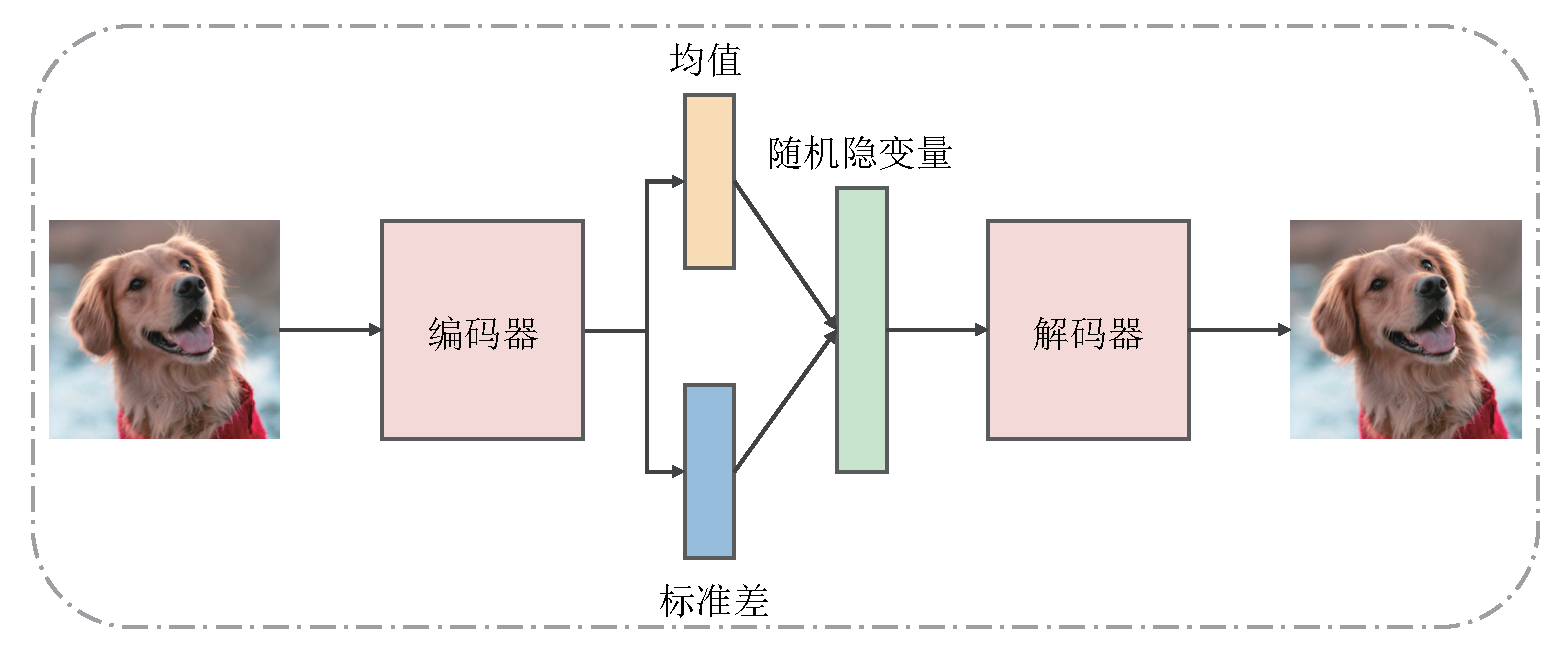
\includegraphics[width = \textwidth]{vae2}
\vspace{-1em}
\caption{变分自编码器结构 \label{vae}}
\end{figure}

\section{本文的主要研究内容}
本文主要研究了考虑缺失值对于时间分布和空间分布的影响的交通数据的算法设计问题。本文主要从以下三个方面,来对不完整的交通数据这一复杂的研究对象展开研究:

(1)时间依赖性:交通数据作为一种复杂的多维度时间数据。同一区域的交通状况在不同的时间点是呈现非线性的时间依赖关系,即是当前时刻的观测值和过去时刻的观测值是相互影响的,而不是独立的。同时,由于缺失值的存在的,使得同一区域中的时间数据可能是离散的,即是某一时刻的数值发生丢失,导致原本连续的时间数据变得零散。

(2)空间相关性:普通的交通数据的空间相关性,主要分为短距离的空间相关性,以及长距离的空间相关性。短距离的空间相关性主要是指某个地区交通流入量和邻近区域的交通流入量存在相关性;长距离的空间相关性主要是指由于交通设备的普及,某个区域的交通流入量会与较远区域的交通流入量存在相关性。同时,由于缺失值的存在,往往使得原本存在短距离空间相关性,或者长距离空间相关性发生丢失,导致以往的提取特征的方法效果往往会不好。

(3)缺失不确定性:由于内外因的干扰,交通数据的缺失现象是不可避免的,且数据缺失模式多样,缺失比例随机,这为数据补全带来了巨大的挑战。

针对以上挑战,本文在变分自编码器的基础上,首先设计了专门针对于带有缺失值的交通数据的时间特性的模块Biconvgrui,然后使用了针对于带有缺失值的交通数据的空间分布的卷积模块。且所设计方法实现了较低的填充绝对误差和相对误差。本文的研究工作围绕对于带有缺失值的交通数据的时间特性和空间特性的挖掘展开,具体内容如下:

(1)考虑缺失值对交通数据的时间分布特性影响的算法设计。考虑到城市交通网络可以按照经纬度划分为等距离的栅格图,那么在每个固定的时间区间内,该栅格图可视为包含多通道的图片,本文将一个城市内每日按照固定频率采集的栅格数据视为一段由多个连续帧组成的多通道视频,该处理方式能极大程度上保留原始交通数据的时空信息。同时,考虑到不同时间窗的交通数据会有不同的时间特性,因而选择小时周期,日周期以及周周期三种时间窗口划分交通数据集。在这个基础上,本文提出了一种可以处理多时间流的生成式填充神经网络模型(\textit{MTS-VAE})。该模型通过使用变分自编码器的强大的生成能力来填充交通数据的缺失值,通过学习随机隐变量的高斯分布来高度抽象交通数据的隐含信息。同时使用了多时间流窗口提取交通数据的不同周期的时间信息。为了充分提取包含缺失值的交通数据的时间分布,本文设计了一个特征提取模块,该模块中的Biconvgrui可以有效建模不完整交通数据的时间分布。同时,本文使用双向自注意力机制,增强卷积模块对于不完整数据中的缺失值和存在值的能力,并对提取的时空特征图在多个维度上进行校正。在开源交通数据集TaxiBJ、BikeNYC和TaxiNYC的实验结果表明,本文提出的填充模型\textit{MTS-VAE}在多种误差指标上都取得了优于主流填充算法的成绩。

(2)考虑缺失值对交通数据的空间分布特性影响的算法设计。虽然MTS-VAE模型使用了专门针对于带有缺失值的交通数据的时间特性的模块\textit{Biconvgrui},可以很好地建模不完整交通数据的时间分布。但是,考虑到缺失值的存在会使得交通数据的空间特性发生变化,使用普通的卷积模块很难有效地提取不完整数据的空间特征。同时,不同时间窗的交通数据间也是存在时间依赖性的,不能简单地将不同时间窗的交通数据视作相互独立的时间流数据。基于此,本文设计了一种多层Attention-Biconvgrui时空变分自编码器(\textit{MCST-VAE})。首先,该方法使用轻量级的双向注意力图的卷积模块替换原来的卷积模块,来达到能够动态更新掩膜的目的。其次,使用多层的Biconvgrui模型对三个时间窗(小时周期,日周期和周周期)的交通数据进行处理,得到一个包含大量存在信息的数据特征。最后,使用赛尔维斯特标准化流(Sylvester Normalizing Flows,SNFs)的变分自编码器替换基础的变分自编码器模型,使得模型可以通过学习随机隐变量的非高斯分布来高度抽象交通数据的隐含信息。最后,本文优化了模型的目标函数,使其不仅能填充输入数据的缺失值,且能保证高层语义信息的准确性。在上文提到的数据集上的实验结果显示,本文设计的模型\textit{MCST-VAE}的填充效果优于交通领域主流的算法,能够逐帧地对交通栅格数据进行精细化填充。
%,并且下游预测任务在使用此方法填充的数据集后能有效地提高预测的准确性
\section{本文的组织结构}

本论文一共分为四个章节。

第一章对本文的研究现状和研究背景进行详细的介绍。本章首先介绍了智能交通的基本理念,以及在智能城市中的重要地位,然后介绍了完整数据在智能交通应用中的重要性,进而强调对不完整的交通数据进行填充处理的必要性。随后介绍了国内外基于统计机器学习、神经网络和变分自编码器技术相关的缺失值填充算法的研究现状。最后重点描述了本文所面临的的一些挑战和主要的研究内容。

第二章阐述了研究本文所需要具备的相关理论基础和技术背景。本章节首先介绍了城市交通数据的一些相关的定义,同时对缺失数据的缺失机制进行了说明。然后对多种卷积操作进行介绍,并对Convgru模型进行说明。最后对目前较为流行的变分自编码器,以及其相关的延伸模型的原理进行介绍。通过本章相关知识的介绍,有助于读者理解第三、四章的算法设计内容。

第三章介绍了考虑时间缺失值分布特性的填充算法设计。本章先对现有的交通数据缺失值的填充算法进行介绍,分析了它们存在的不足之处。接着介绍了对于城市交通雷达数据的处理方式,随后提出了考虑了时间缺失值分布特性的多时间流变分自编码器的填充模型,并对模型的目标函数进行了详细的介绍。最后,本章介绍了所用的开源交通数据集、评价指标、实验设置,并对实验结果进行了分析总结。

第四章介绍了考虑空间缺失值分布特性的填充算法设计。本章节首先对上一章节的内容进行总结,并说明构建考虑空间缺失值分布特性的填充算法的必要性。接着提出了一种考虑空间缺失值分布特性的变分自编码器,并在传统的变分自编码器的基础上使用了标准化流编码器,以优化模型的生成效果。最后,本章分析了所提出了方法与对比方法的模型复杂度以及在公共数据集上的实验结果。

最后,结论部分对本文的研究内容和成果进行总结,对未来的可拓展研究的内容进行展望。

% Local Variables:
% TeX-master: "../thesis"
% TeX-engine: xetex
% End:
% !Mode:: "TeX:UTF-8"

\chapter[相关理论和技术介绍]{背景知识和相关技术介绍}[xxx]
% 10-11页
\section{引言}
本章将会对利用变分自编码器进行交通数据缺失值填充所需要的前置知识进行介绍。本章首先介绍城市交通网络中出现的一些重要的名词定义,然后介绍了神经网络中常用的卷积运算,接着介绍了标准化流技术,最后本章着重描述了用于重建数据的原始变分自编码器模型。
\section{城市交通网络相关理论}
\subsection{交通栅格数据}
交通流量是城市交通网络的重要组成部分,它提供了特定路段或区域中的空间拥堵信息,这在城市网络分析中十分重要,因为交通流量的大小会影响交通工具的行驶时间,从而影响交通管制单位的行为决策或城市居民的出行计划。

根据不同的粒度和语义信息可以对一个区域做出多种定义,本文中主要采用以下的方式来定义城市交通区域。
\begin{definition}[\cite{zhang2017deep}(区域)] 将一个城市的经纬度转化成平面坐标,并按照规定间距等距离将整个城市地图划分为长为$H$,宽为$W$的网格图$\mathcal{G}$,图中的每个格子$(h, w)$代表一个区域,如图\ref{gridmap}所示。

\end{definition}
\begin{figure}[h]
\centering
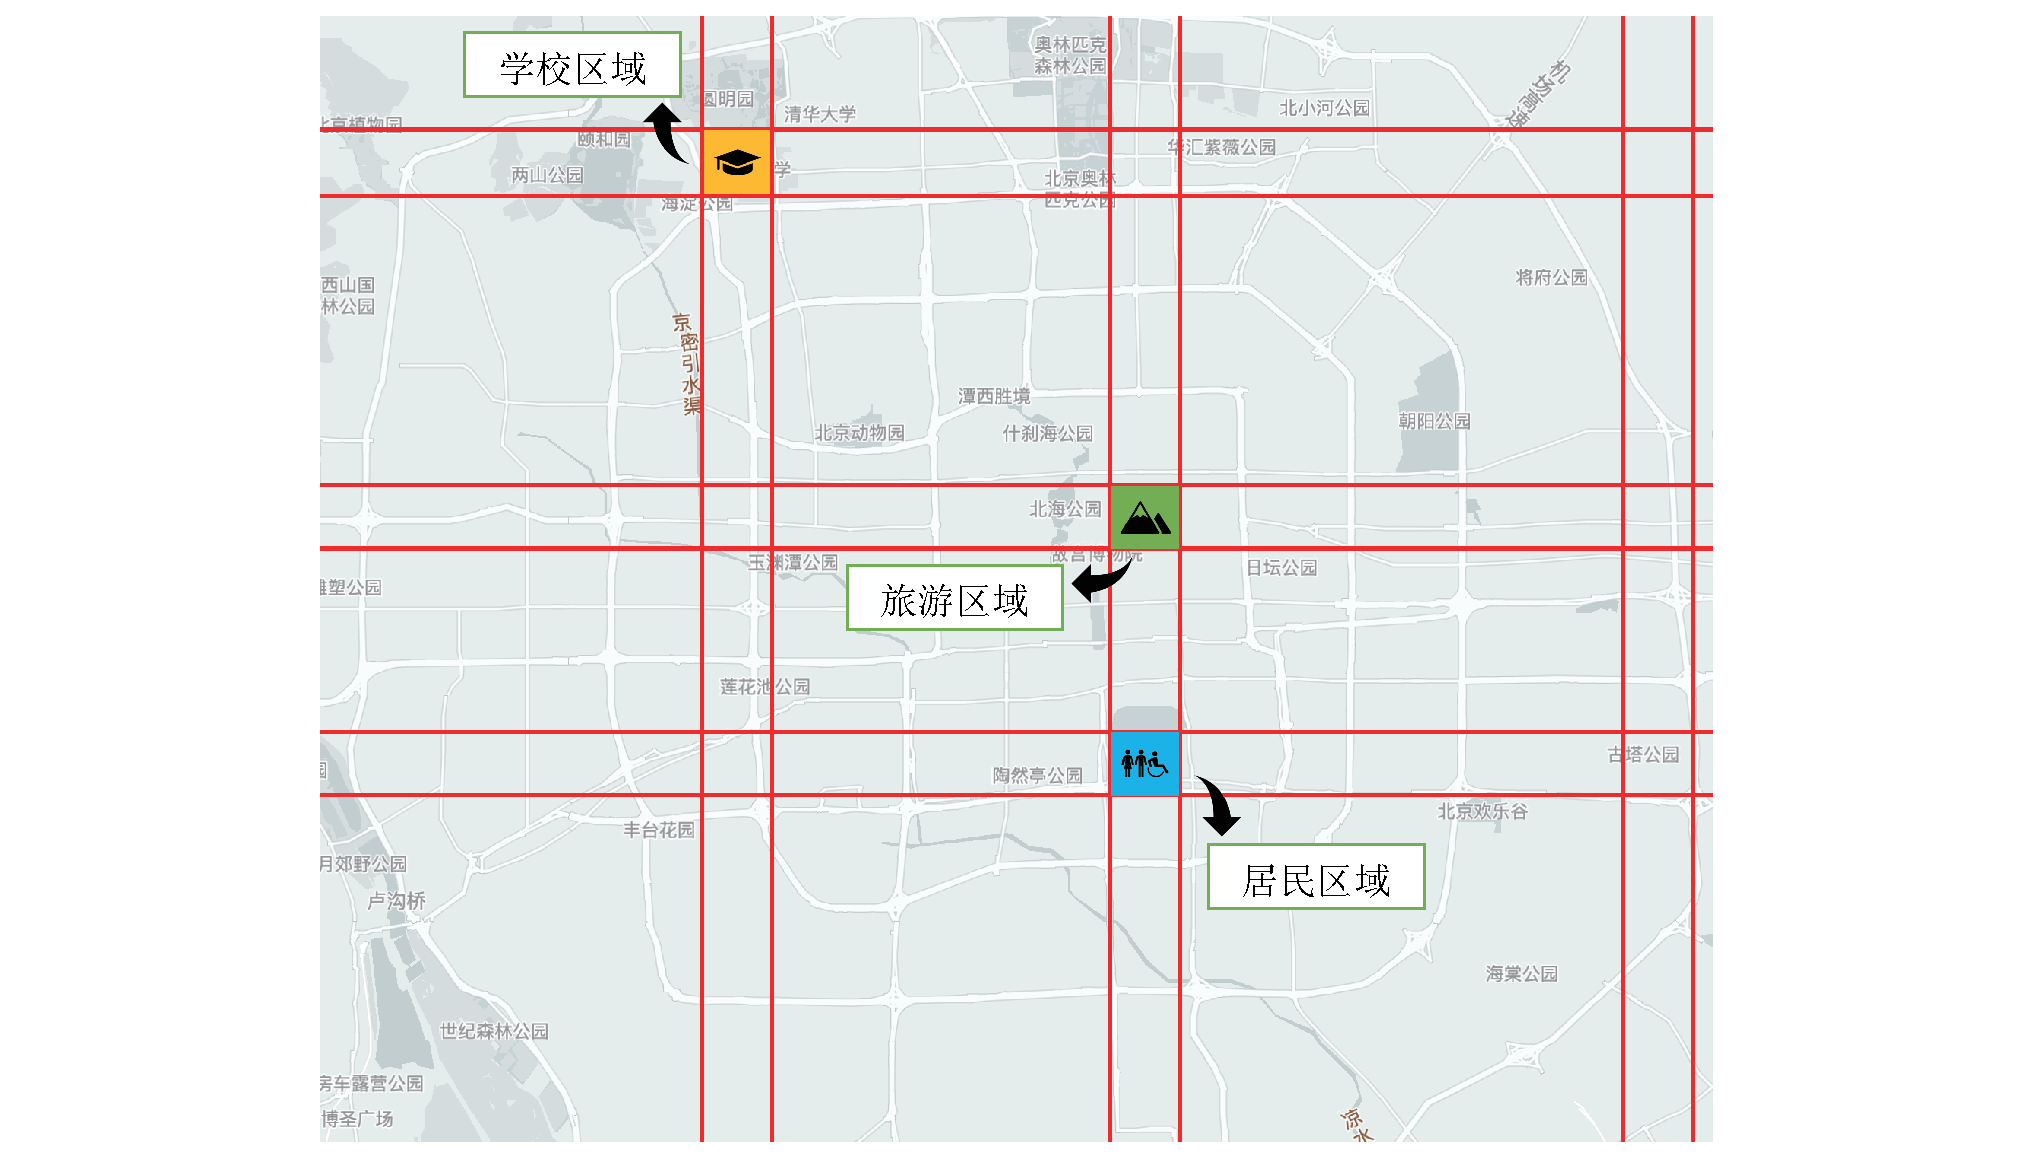
\includegraphics[width = 0.9\textwidth]{gridmap}
\vspace{0.5em}
\caption{城市区域网格图 \label{gridmap}}
\end{figure}

\begin{definition}[\cite{zhang2017deep}(区域出入流量)] \label{def_flow}
给定第$t$个时间区间内的人群轨迹集合$\mathbb{P}_{t}$,在图$\mathcal{G}$的区域$(h, w)$内,区域交通出入流量可以分别用下式定义。
\begin{equation}
	x^{in, t, h, w} = \sum_{Tr_{t} \in \mathbb{P}_{t}}\left|\left\{k>1 \mid l_{k-1} \notin(h, w) \wedge l_{k} \in(h, w)\right\}\right|
\end{equation}
\begin{equation}
	x^{out, t, h, w} = \sum_{Tr_{t} \in \mathbb{P}_{t}}\left|\left\{k \geq 1 \mid l_{k-1} \in(h, w) \wedge l_{k} \notin(h, w)\right\}\right|,
\end{equation}
其中$Tr_{t}: l_{1} \rightarrow l_{2} \rightarrow \cdots \rightarrow l_{|Tr_t|}$表示集合$\mathbb{P}_t$中的一条轨迹,且$l_k$表示地理坐标;$l_k \in(h, w)$表示坐标$l_k$位于区域$(h, w)$内,反之亦然;$| \cdot |$表示集合的基数。
\end{definition}

\begin{figure}[htbp]
\centering
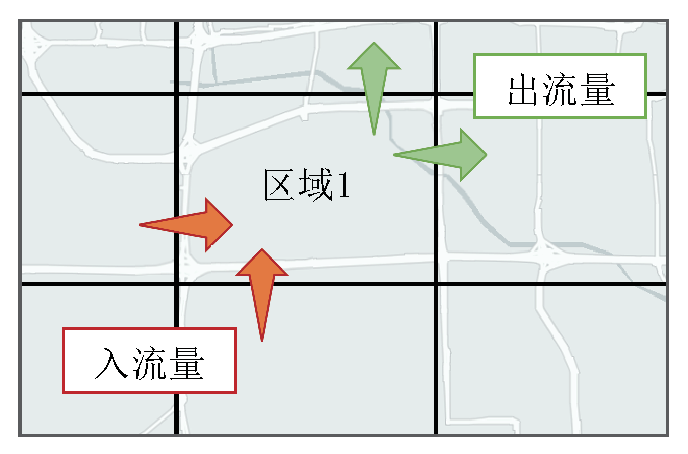
\includegraphics[width = 0.4\textwidth]{region}
\vspace{0.5em}
\caption{区域出入流量 \label{region}}
\end{figure}
也就是说,区域入流量是指在给定的时间区间内从其他地点进入此区域的人流量总数,区域出流量是指在给定的时间区间内从该区域离开的人流量总数,如图\ref{region}所示。两个指标记录了不同区域间人群的转移情况,因此,挖掘其中的信息对于交通管制和交通风险评估意义重大。区域出入流量可由交通工具数量、路上行人数等统计得到,常用的测量手段有使用手机信号来定位行人的轨迹、使用GPS来定位出租车的位置,图\ref{measure}给出了形象的描述。

\begin{figure}[htbp]
\centering
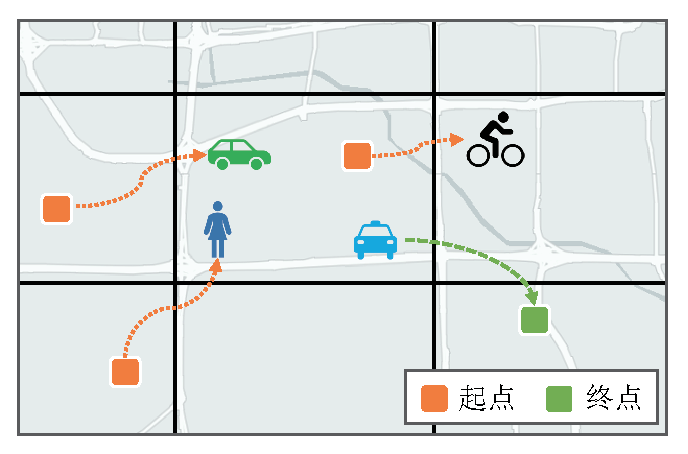
\includegraphics[width = 0.5\textwidth]{measure}
\vspace{0.5em}
\caption{交通流量测量 \label{measure}}
\end{figure}

%\begin{figure}[htbp]
%\centering
%\begin{minipage}[t]{0.42\textwidth}
%\centering
%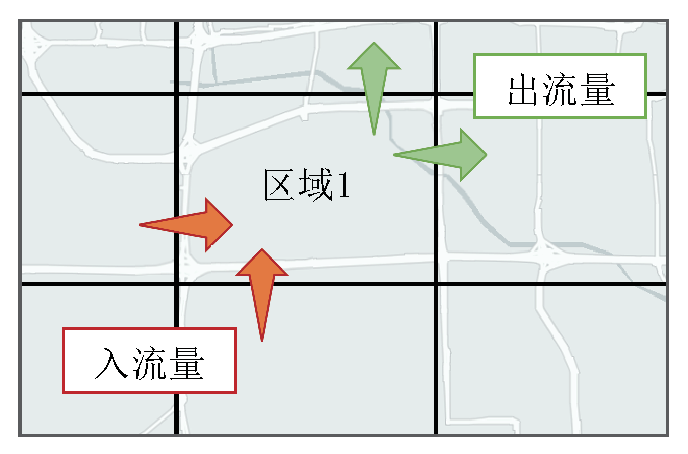
\includegraphics[width=\textwidth]{region}
%%\vspace{0.1em}
%\caption{区域出入流量 \label{region}}
%\end{minipage}
%\centering
%\begin{minipage}[t]{0.42\textwidth}
%\centering
%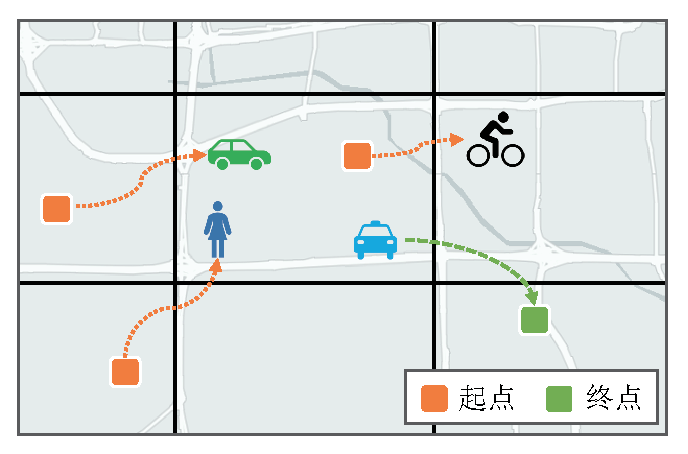
\includegraphics[width=\textwidth]{measure}
%%\vspace{0.1em}
%\caption{交通流量测量 \label{measure}}
%\end{minipage}
%\end{figure}

Atluri\cite{atluri2018spatio}等人将时空数据分为四大类,分别包括事件数据、轨迹数据、点参考数据和栅格数据。本文将人群轨迹数据转换成栅格数据,即在第$t$个时间区间内,图$\mathcal{G}$内所有的交通出入流量可以被表示成一个张量$x_t\in\mathbb{R}^{2 \times H \times W}$,其中$x_t[0,h,w]=x^{in,t,h,w}$,$x_t[1,h,w]=x^{out,t,h,w}$。

\subsection{数据缺失机制}
文献\inlinecite{little2019statistical}指出,缺失值填充过程旨在学习未被观测到的缺失数据的概率分布,一般可将缺失值的缺失模式分为以下三种情况:

(1)完全随机缺失(Missing Completely At Random,MCAR)。该缺失模式是指缺失值的产生是完全随机的,即数据的缺失的概率分布独立于任何观测变量和其它缺失变量。本文通过采用百分位阈值的方式,随机采样固定百分比的位置作为缺失值来模拟该机制。

(2)随机缺失(Missing At Random,MAR)。该缺失模式缺失值的产生不是完全随机的,即缺失值依赖于其它观测变量,但不依赖于缺失变量。

(3)非随机缺失(Missing Not At Random,MNAR)。该缺失模式缺失值的产生依赖于观测变量和缺失变量自身。它一般由传感器的长期故障所导致,故无法通过算法来很好地还原原始数据,本文不考虑此种缺失模式。


%\section{神经网络激活函数}
%神经网络中的全连接层相当于对数据进行仿射变换,那么叠加多个全连接层的效果等价于将其压缩成一个全连接层,这样增加网络层数并不能提升网络的拟合能力,因此有必要在层与层之间添加非线性的激活函数来强化神经网络的学习能力。以下公式介绍了本文中所用到的激活函数。
%\begin{equation}
%	Sigmoid(x)=\frac{1}{1+e^{-x}}
%\end{equation}
%\begin{equation}
%	Tanh(x)=\frac{e^x-e^{-x}}{e^x+e^{-x}}
%\end{equation}
%\begin{equation}
%	ReLU(x)=max(0, x)
%\end{equation}
%\begin{equation}
%LeakyReLU(x)=
%\begin{cases}
%x, & x>0\\
%-\alpha x, & x \le 0, \alpha \textgreater 0.
%\end{cases}
%\end{equation}
%
%在本文的研究工作中,主要将$Sigmoid$函数和$Tanh$函数用于输入和输出数据值域的缩放,而$ReLU$函数\cite{krizhevsky2012imagenet}和$LeakyReLU$函数\cite{maas2013rectifier}则用于神经网络内部,主要原因是后两者解决了前者梯度消失的问题,且能加速模型的计算速度。

\section{卷积运算}
卷积神经网络一直是深度学习蓬勃发展的核心,但它与全连接网络不同,它的输出不仅取决于输入的大小,还取决于网络层内部多个参数的设定,因此,有必要对其进行介绍。下面将对普通2D卷积、转置卷积、3D卷积进行阐述。
\subsection{普通卷积和转置卷积}
从数学定义的角度来看,普通卷积是为了诸如信号处理,求两个随机变量和的分布等而定义的运算。并且,数学定义中的卷积核的值是已经被确定了,因此需要将卷积核(权重矩阵)翻转后,再同原来的矩阵数据作对乘操作,同时按照一定的操作顺序(即从上到下,从左到右的顺序),在原始的矩阵数据上进行重复滑动计算。在深度学习中,普通卷积的卷积核的值可以通过神经网络的反向传播进行学习,因而在深度学习中的卷积核并没有翻转这一操作。一个卷积核对应一个矩阵变换操作,多个卷积核对应多个函数映射操作,可以拓展到多个随机分布,这样可以从输入的矩阵数据中提取到更多的随即特征。同时,卷积核权重的更新过程可以看成是一个复杂函数拟合的过程。

\vspace{1em}
\begin{figure}[htbp] 
\centering
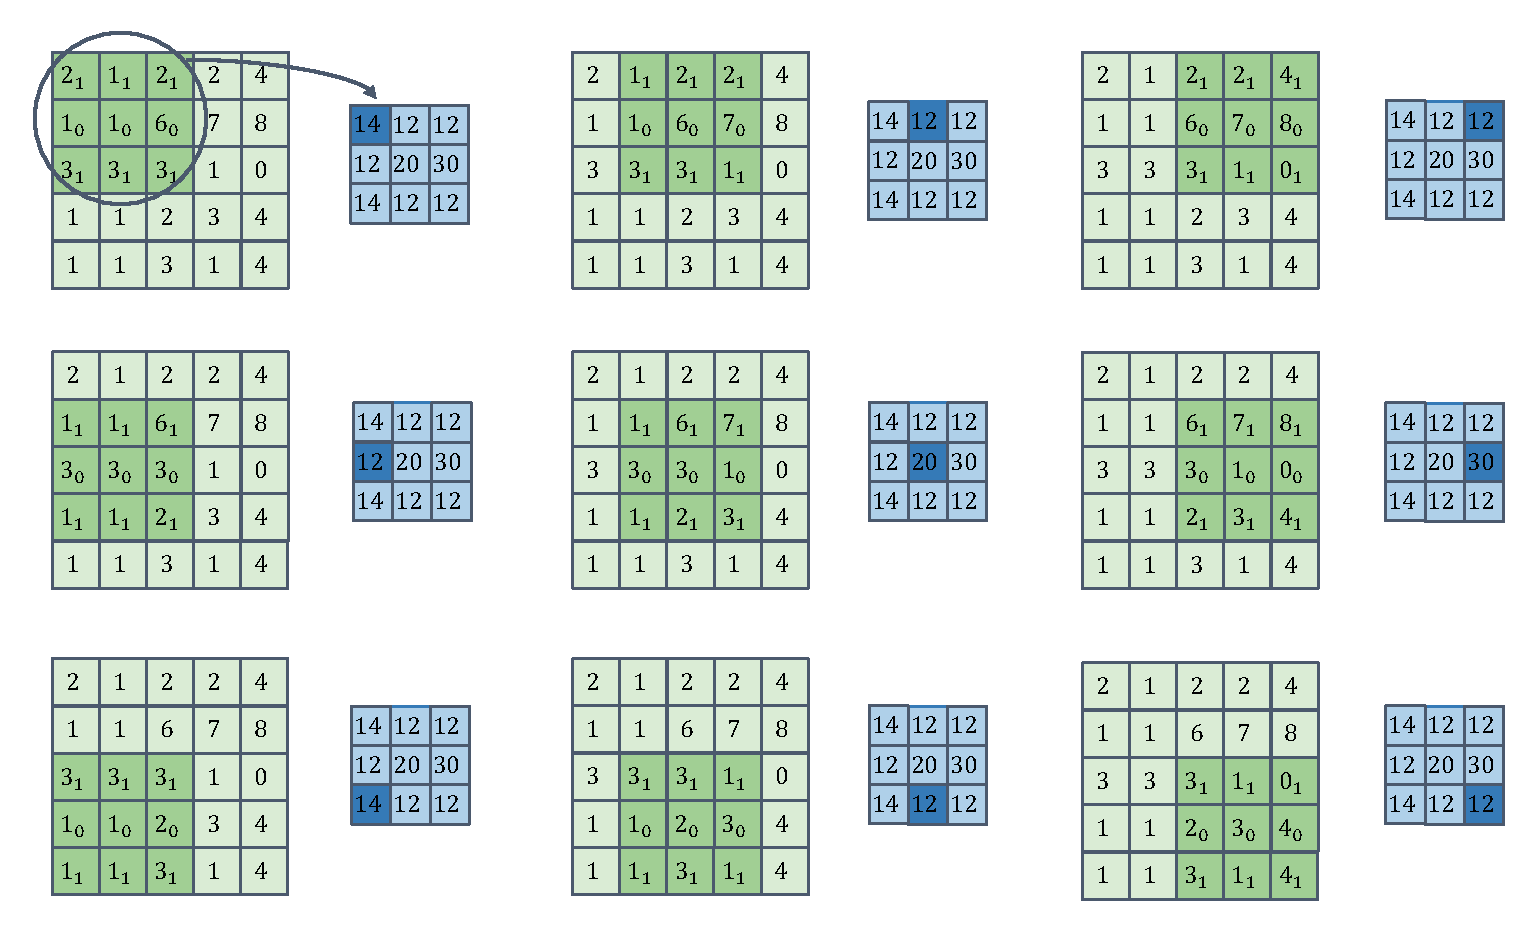
\includegraphics[width = \textwidth]{conv}
\vspace{-0.5em}
\caption{2D卷积运算\label{conv2d}} 
\end{figure}

其运算形式如下所示:
\begin{equation}
	O(i, j) = \sum_{m} \sum_{n} F(m, n) I(i+m, j+n).
\end{equation}

转置卷积(Transposed Convolution)与一般也叫做反卷积,其具体的操作过程如图\ref{tranconv}所示。。它通常用于将输入的特征图进行放大还原成原始大小。因而经常与卷积操作进行组合。卷积加上转置卷积的基础模型,也叫做自编码器。虽说转置卷积的操作结果是将卷积操作处理得到的特征图还原为原始数据大小,但是这并不意味着转置卷积就是卷积的反向操作。因为即使在普通卷积上使用同一个卷积核进行操作,也不可能保证得到的结果就和原始数据的一模一样。转置卷积的操作一般是先按照一定的比例通过填充补零的操作来扩大输入图像的尺寸,接着再按照一定的顺序(即从上到下,从左到右的顺序),移动卷积核,在进行普通卷积得到相应的结果。过程如图\ref{tranconv}所示。

\begin{figure}[htbp]
\centering
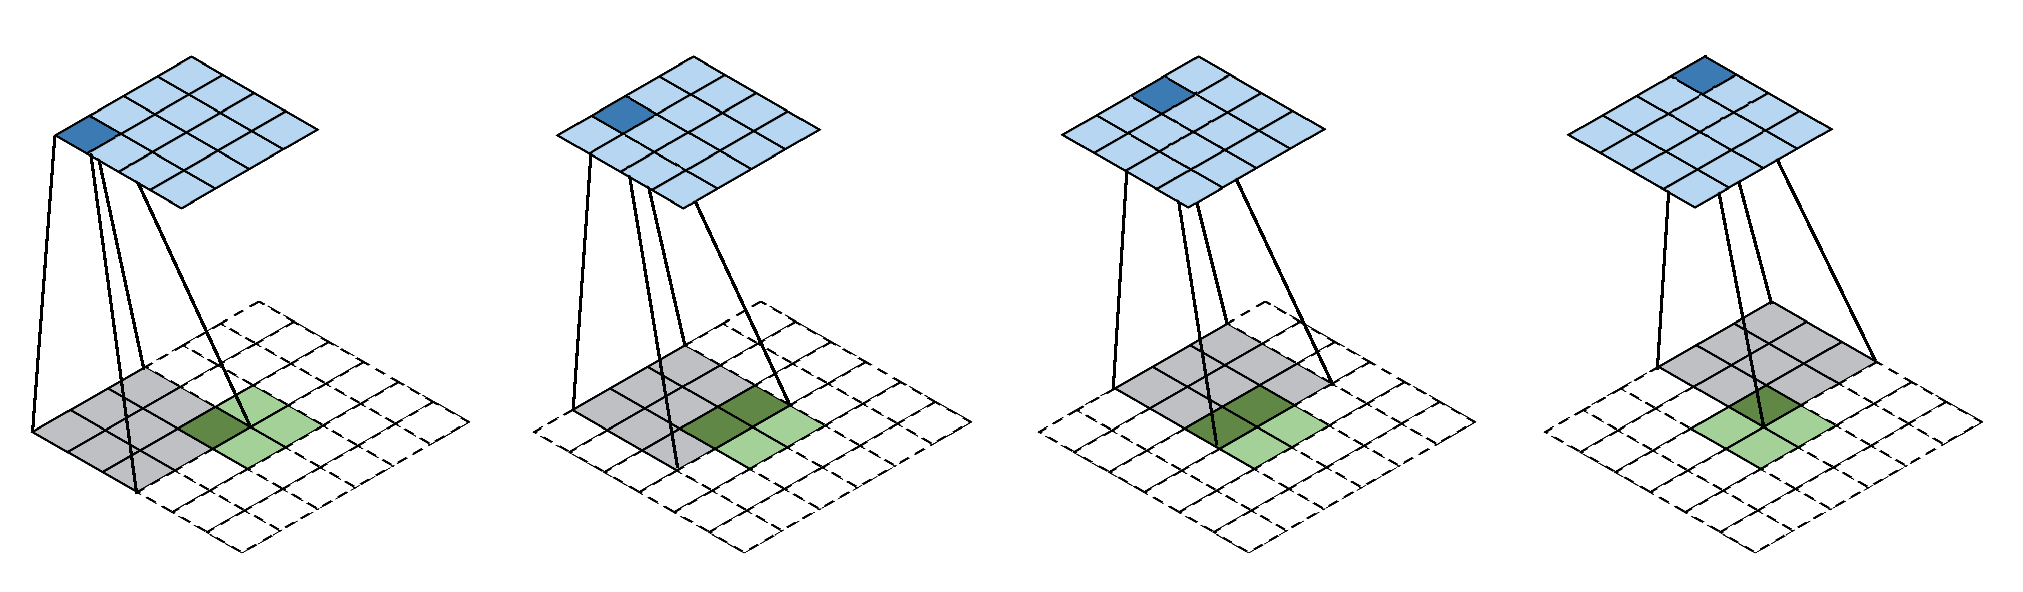
\includegraphics[width = \textwidth]{transpose_conv}
\vspace{0.25em}
\caption{转置卷积过程 \label{tranconv}}
\end{figure}

对一个输入图线进行转置卷积操作后得到的特征图$O$的尺寸$H_{out}$可由如下式子计算得出:
\begin{equation}
	H_{out}=(H_{in}-1)s - 2p+k,
\end{equation}
基于转置卷积能恢复形状的特性,它被广泛应用于图像的上采样操作,尤其在自编码器结构中的解码器和生成对抗网络中的生成器中使用较为频繁。

\subsection{3D卷积}
从前面的介绍中可以得知,2D卷积(即普通卷积)主要用于处理二维数据,比如静态图片,时序数据等。当使用2D卷积处理类似视频这些连续的图像数据,或者其它时空数据时,就需要把数据压缩成二维数据。最常使用的方式主要是把RGB通道维度同时间维度压缩成一个单维度。但是这样却会使得卷积无法准确地区分通道特征和时间特征,导致无法获取到准确的特征。3D卷积于2010年被Shuiwang Ji团队\cite{ji20123d}所提出,主要是应用在处理时空数据的特征提取问题上。

如图\ref{3Dconv}所示,3D卷积的卷积核比2D卷积多了一个时间维度,因此能保留输入图像的时间信息。

对一个输入视频进行3D卷积操作,一般需要指定以下参数:

(1)输入视频$I$的尺寸$W_{in}$

(2)卷积核$F$的尺寸$k$

(3)填充(padding)大小$p$

(4)步长(stride)大小$s$

那么经过3D卷积运算后得到的特征图$O$的尺寸$W_{out}$可由如下式子计算得出:
\begin{equation}
	W_{out}=\bigg{\lfloor} \frac{W_{in}+2p-k}{s} \bigg{\rfloor} + 1,
\end{equation}

另外$O$中每一个元素$O(t,i,j)$可由以下卷积操作计算得出:
\begin{equation}
	O(t, i, j) = \sum_{l} \sum_{m} \sum_{n} F(l, m, n) I(t+l, i+m, j+n).
\end{equation}

自从3D卷积被提出来后,它就被广泛应用于行为识别\cite{tran2018closer},视频修复\cite{wang2019video}等领域。同样的,交通数据作为一种常见的时空数据,也包含了时间维度,以及空间维度。因而可以将3D卷积应用于叫用数据挖掘任务\cite{yu20193d, guo2019deep}。
\begin{figure}[htbp] 
\centering
\includegraphics[width = 0.6\textwidth]{3Dconv}
\caption{3D卷积 \label{3Dconv}}
\end{figure}

\section{ConvGRU}
由于RNN系列模型(包括GRU模型以及LSTM模型)在处理时序数据时的优越表现,因而它被广泛应用到与时序相关的问题中,比如股价预测问题等。普通的GRU模型是在LSTM模型的基础上将相关门电路的功能进行整合简化,只保留了重置门电路和更新门电路。极大程度上降低了模型的训练难度。GRU模型的更新公式如下所示:

虽然RNN系列模型在处理时序数据时表现出优越的性能。但是由于其自身模型的设计,即在神经元的连接部分使用全连接层处理数据。限制了它处理时空数据的能力。为了使得RNN系列模型能够进一步处理时空数据这种三维数据。Shixingjian博士团队提出了新的RNN系列模型ConvLSTM以及ConvGRU模型。ConvGRU模型的改进之处主要是将模型中的全连接操作更换为卷积操作,从而使得模型具备处理时空数据的能力。ConvGRU模型的更新公式如下:

自从新的RNN系列模型ConvLSTM以及ConvGRU模型被提出来之后,它就被广泛应用到天气预测问题,以及视频预测等一系列时空数据的问题中。交通数据作为一种寻常的时空数据,ConvGRU模型也可以应用到交通数据的缺失值填充问题中。

\section{标准化流技术}
标准化流(Normalizing Flows)的核心思想是将一个相对简单,也就是易于采样的概率分布通过一系列可逆的参数化转换映射成一个更加灵活的概率分布,如图\ref{normal_flow}所示。下面介绍如何计算一个随机变量的概率密度函数,该随机变量由另外的随机变量变换而来。

\begin{figure}[htbp]
\centering
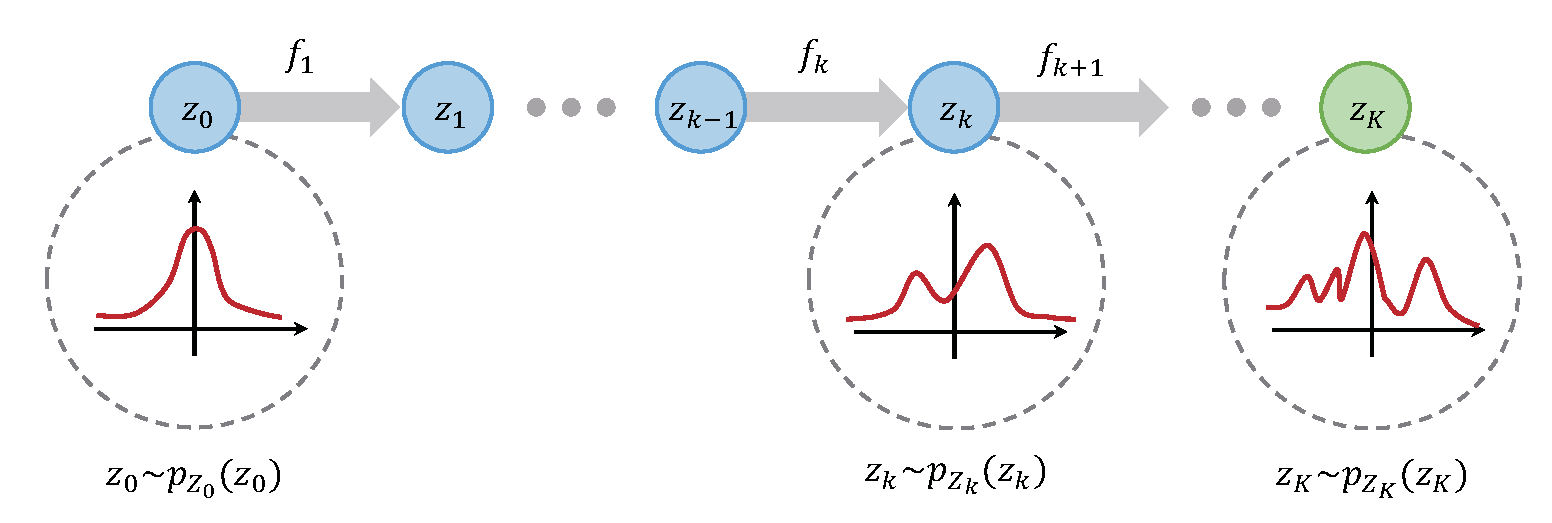
\includegraphics[width = 0.9\textwidth]{flow}
\vspace{1em}
\caption{标准化流 \label{normal_flow}}
\end{figure}

假设随机变量$Z \in \mathbb{R}^n$的概率密度函数已知且易于计算(Tractable),记为$p_Z: \mathbb{R}^n \rightarrow \mathbb{R}$,另一个待求的随机变量$X \in \mathbb{R}^n$密度函数为$p_X: \mathbb{R}^n \rightarrow \mathbb{R}$,二者之间存在可逆的映射关系$f:\mathbb{R}^n \rightarrow \mathbb{R}^n$,即满足$X=f(Z)$且$Z=f^{-1}(X)$,则有
\begin{equation}
\begin{split}
	p_X(x) & = p_Z(f^{-1}(x))\bigg | det\bigg (\frac{\partial f^{-1}(x)}{\partial x}\bigg )\bigg | \\
	& = p_Z(z)\bigg | det\bigg (\frac{\partial f(z)}{\partial z}\bigg )\bigg |^{-1}, \\
\end{split}
\end{equation}
其中,$\frac{\partial f^{-1}(x)}{\partial x}$和$\frac{\partial f(z)}{\partial z}$分别为函数$f^{-1}$和$f$的雅克比矩阵。

不失一般性,若将$K$个可逆变换$f_1, f_2, ...,f_{K}$做复合运算$f_{K} \circ \cdots \circ f_{k}\circ \cdots \circ f_{1}(z_{0})$,可以得到如下表达式:
\begin{equation}
	p_{Z_K}(z_K) = p_{Z_0}(z_0)\prod_{k=1}^{K}\bigg | det\bigg (\frac{\partial f_{k}(z_{k-1})}{\partial z_{k-1}}\bigg )\bigg |^{-1},
\end{equation}
两边取对数后得到:
\begin{equation}
	\log p_{Z_K}(z_K) = \log p_{Z_0}(z_0) - \sum_{k=1}^{K}\log \bigg | det\bigg (\frac{\partial f_{k}(z_{k-1})}{\partial z_{k-1}}\bigg )\bigg |.\label{nf_func}
\end{equation}

根据上面的介绍,标准化流可以将一个简单的分布转换成较为复杂的分布,因此,它能被应用于随机梯度变分推断中来近似更加灵活的后验分布\cite{rezende2015variational},本论文第三章中所提出的算法中将使用该技术提升模型的表达能力。

从式子\eqref{nf_func}中不难发现,链式变换主要的计算量来自于每个可逆函数$f_k$的雅克比行列式,已知一个$n \times n$的雅克比行列式的计算复杂度为$O(n^3)$,只要其能被快速地计算,那么便可通过标准化流技术得出最新的随机变量的概率密度。目前已有大量关于标准化流的研究工作围绕如何高效地计算雅克比行列式展开,有兴趣的读者可阅读综述文献\inlinecite{kobyzev2020normalizing}。
\section{变分自编码器}
\subsection{深度隐变量模型}
深度隐变量模型(Deep Latent Variable Models,DLVMs)是一类包含隐变量的有向概率图模型,如图\ref{dlvm}所示,它表示观测变量$x$和隐变量$z$的联合概率分布$p_{\theta}(x, z)$。
关于观测变量$x$的边缘概率分布$p_{\theta}(x)$如下:
\begin{equation}
	p_{\theta}(x)=\int p_{\theta}(x, z) d z, \label{int}
\end{equation}
由于式子\eqref{int}中包含积分运算,这导致无法计算$p_{\theta}(x)$,那么也就不能通过求微分来对参数$\theta$进行更新,进而无法计算$z$的后验概率分布$p_{\theta}(z|x)$。变分推断技术允许通过引入近似后验的手段来解决此问题,将在下一小节中介绍。

%\begin{figure}[htbp]
%\centering
%\begin{minipage}[t]{0.44\textwidth}
%\centering
%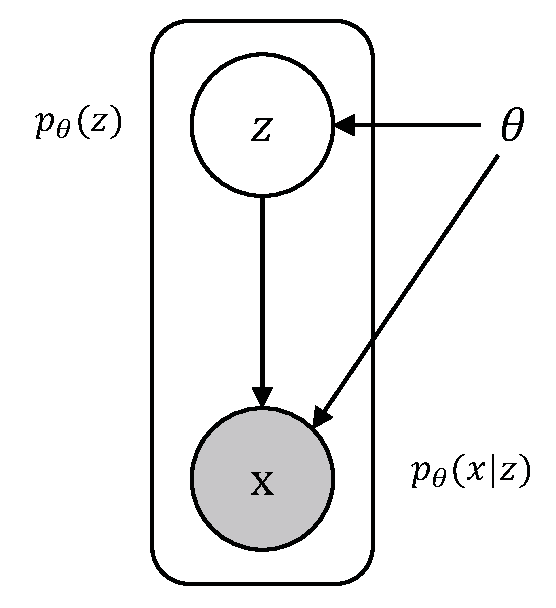
\includegraphics[width = 0.79\textwidth]{dlvm}
%\vspace{1em}
%\caption{深度隐变量模型的概率图 \label{dlvm}}
%\end{minipage}
%\centering
%\begin{minipage}[t]{0.44\textwidth}
%\centering
%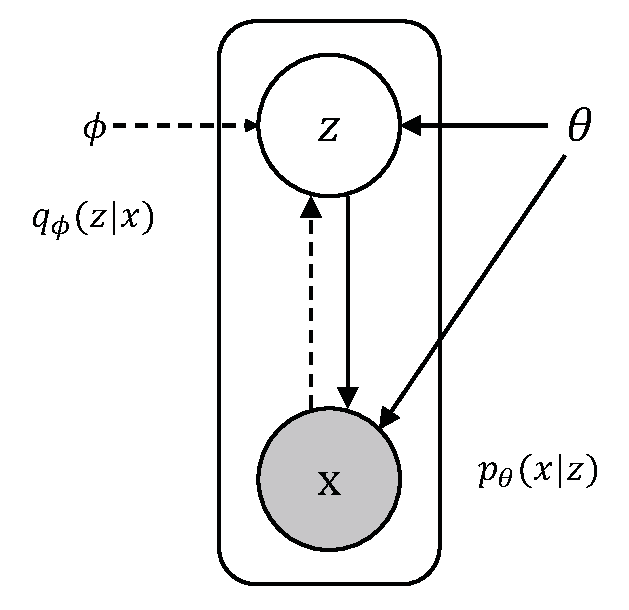
\includegraphics[width = 0.9\textwidth]{vaeg}
%\vspace{1em}
%\caption{变分自编码器的概率图 \label{vaeg}}
%\end{minipage}
%\end{figure}

\subsection{近似后验}
为了解决深度隐变量模型中无法求解后验概率分布$p_{\theta}(z|x)$的问题,Kingma\cite{kingma2013auto}等人提出了变分自编码器架构,即使用参数化的推断模型$q_{\phi}(z|x)$(编码器)来近似$p_{\theta}(z|x)$,其概率图如图\ref{vaeg}所示。我们一般使用神经网络来参数化近似后验。例如,假设后验分布满足各项同性的高斯分布,则有:
\begin{equation}
\begin{split}
	(\mu, log\sigma) & = Encoder_{\phi}(x) \\
	q_{\phi}(z|x) & = \mathcal{N}(z;\mu, diag(\sigma)) .
\end{split}
\end{equation}

\begin{figure}[htbp] 
	\centering 
	\subfigure[深度隐变量模型]{
		\begin{minipage}[htbp]{0.44\textwidth}
			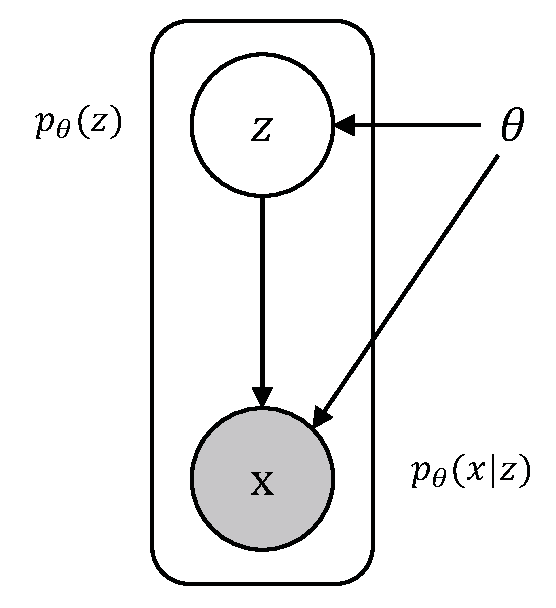
\includegraphics[width=0.79\textwidth]{dlvm} \label{dlvm}
		\vspace{0.5em}
		\end{minipage}	
	}
	\subfigure[变分自编码器]{
		\begin{minipage}[htbp]{0.44\textwidth}
			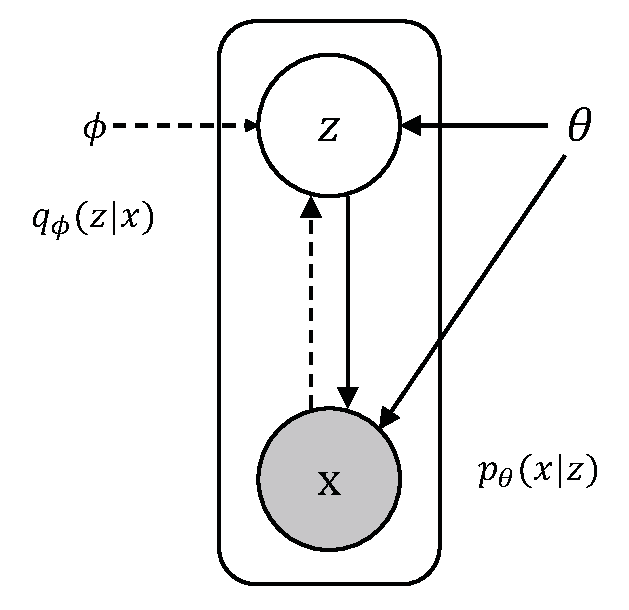
\includegraphics[width=0.9\textwidth]{vaeg} \label{vaeg}
		\vspace{0.5em}
		\end{minipage}
	}
	\caption{概率图}
\end{figure}

\subsection{变分下界}
变分自编码器的目标函数通过最大化观测变量$x$的边缘似然得到,具体推导过程如下所示:
\begin{equation}
\begin{split}
	\log{p_{\theta}(x)} & = \log{p_{\theta}(x, z)} - \log{p_{\theta}(z|x)} \\
	& = \log{\frac{p_{\theta}(x, z)}{q_{\phi}(z|x)}} + \log{\frac{q_{\phi}(z|x)}{p_{\theta}(z|x)}} \\
	& = \underbrace{\mathbb{E}_{q_{\phi}(z|x)}\bigg[\log{\frac{p_{\theta}(x, z)}{q_{\phi}(z|x)}}\bigg]}_{\mathcal{L}_{\theta, \phi}(x)} + \underbrace{\mathbb{E}_{q_{\phi}(z|x)}\bigg[\log{\frac{q_{\phi}(z|x)}{p_{\theta}(z|x)}}\bigg]}_{D_{KL}(q_{\phi}(z|x)\parallel p_{\theta}(z|x))\geq 0} \\
	& \geq \mathbb{E}_{q_{\phi}(z|x)}\bigg[\log{\frac{p_{\theta}(x, z)}{q_{\phi}(z|x)}}\bigg], \label{likehood}
\end{split}
\end{equation} 
上式第二项为$q_{\phi}(z|x)$与$p_{\theta}(z|x)$的Kullback-Leibler散度,它非负并且只有两个分布相等时等于0;上式第一项为$\log{p_{\theta}(x)}$的下界,又叫证据下界(Evidence Lower Bound,ELBO),将其展开又可得到:
\begin{equation}
	\mathcal{L}_{\theta, \phi}(x) = \log{p_{\theta}(x)} - D_{KL}(q_{\phi}(z|x)\parallel p_{\theta}(z|x)). \label{elbo}
\end{equation}

从式子\eqref{likehood}和式子\eqref{elbo}中可以发现,KL散度$D_{KL}(q_{\phi}(z|x)\parallel p_{\theta}(z|x))$决定了两种距离,第一是近似后验$q_{\phi}(z|x)$与后验$p_{\theta}(z|x)$的距离,第二是边缘似然$\log{p_{\theta}(x)}$与证据下界ELBO的距离,因此,只要保证$D_{KL}(q_{\phi}(z|x)\parallel p_{\theta}(z|x))$足够小,那么ELBO就越接近$p_{\theta}(z|x)$,也就越能代表它作为变分自编码器的目标函数。

\subsection{变分下界的梯度下降优化}
对于变分自编码器的目标函数$\mathcal{L}_{\theta, \phi}(x)$,可以采用随机梯度下降(Stochastic Gradient Descent,SGD)来更新参数$\theta$ 和 $\phi$。

参数$\theta$的梯度很容易求得:
\begin{equation}
	\begin{split}
		\nabla_{\theta}\mathcal{L}_{\theta, \phi}(x) &= \nabla_{\theta} \mathbb{E}_{q_{\phi}(z|x)}[\log{p_{\theta}(x, z)} - \log{{q_{\phi}(z|x)}}] \\
		&= \mathbb{E}_{q_{\phi}(z|x)}[\nabla_{\theta}(\log{p_{\theta}(x, z)} - \log{{q_{\phi}(z|x)}})] \\
		&\approx \nabla_{\theta}(\log{p_{\theta}(x, z)}).
	\end{split}
\end{equation}

但参数$\phi$的梯度因为ELBO的期望包含了后验分布$q_{\phi}(z|x)$,而它是关于参数$\phi$的函数 ,所以并不易算,如下所示:
\begin{equation}
	\begin{split}
		\nabla_{\phi}\mathcal{L}_{\theta, \phi}(x) &= \nabla_{\phi} \mathbb{E}_{q_{\phi}(z|x)}[\log{p_{\theta}(x, z)} - \log{{q_{\phi}(z|x)}}] \\
		&\neq \mathbb{E}_{q_{\phi}(z|x)}[\nabla_{\phi}(\log{p_{\theta}(x, z)} - \log{{q_{\phi}(z|x)}})],
	\end{split}
\end{equation}
Kingma\cite{kingma2013auto}等人巧妙地使用了重参数化技巧(Reparameterization Trick)使得ELBO可直接进行求导,主要的思想是用一个随机变量$\epsilon$与隐变量$z$建立可导的映射关系$g$,这样就可以将$z$的随机性转移到$\epsilon$上,经重参数化后的ELBO可以被重写成:
\begin{equation}
	\begin{split}
		\mathcal{L}_{\theta, \phi}(x) &= \mathbb{E}_{q_{\phi}(z|x)}[\log{p_{\theta}(x, z)} - \log{{q_{\phi}(z|x)}}] \\
		&= \mathbb{E}_{p(\epsilon)}[\log{p_{\theta}(x, z)} - \log{{q_{\phi}(z|x)}}],
	\end{split}
\end{equation}
其中$z=g(\epsilon, \phi, x)$,$\epsilon$一般服从简单的标准正太分布。

\section{本章小结}
本章介绍了基于变分自编码器进行交通缺失值填充算法设计中所需要用到的背景知识和相关理论。首先介绍了城市交通网络和缺失值填充领域中的一些重要定义,包括栅格数据和数据缺失机制;接下来介绍了神经网络中常见的卷积运算,从普通卷积到转置卷积,最后介绍了能处理时空特征的3D卷积;紧接着介绍了用于提升隐变量分布复杂性的标准化流技术;最后着重阐述了变分自编码器的相关理论,从概率图模型的角度讲述了其目标函数的由来以及对其目标函数参数的优化,本章内容的阅读有助于读者对之后章节内容的深入理解。


% Local Variables:
% TeX-master: "../thesis"
% TeX-engine: xetex
% End:
% !Mode:: "TeX:UTF-8"

\chapter[考虑时间缺失值分布特性的填充算法设计]{考虑时间缺失值分布特性的填充算法设计}[考虑时间缺失值分布特性的填充算法设计]
% 15页
\section{引言}
本章主要研究考虑时间缺失值分布特性的填充算法设计。交通数据中的缺失值会改变其时间分布特性,因此,以往的提取时间特征的方法不适用于提取这种带有缺失值的数据的时间特征。为了解决这个问题,本章提出了一种全新的生成式填充神经网络,即多时间流变分自动编码器(\textit{MTS-VAE})。该模型在变分自编码器的基础上,加入了改进的Biconvgrui模块,可以有效提取带有缺失值的交通数据的时间特征。同时,加入改进的双向注意力机制,提高了模型有效区分缺失值和观测值的能力。在三个开源交通数据集上的实验结果显示,本章所提出的填充算法在考虑时间缺失值分布特性的缺失值填充任务上具有优良的填充准确率。

%本章的各节结构如下:\ref{sec3_2}节对问题进行抽象,给出了问题的数学描述;\ref{sec3_3}节介绍所提出的基于时空注意力机制的变分自编码器填充模型,包括模型整体架构和模型训练;\ref{sec3_4}节介绍如何利用时空变分自编码器进行缺失值填充;\ref{sec3_5}节为本章实验及结果分析,包括对比实验和消融实验;\ref{sec3_6}节为本章小结。

\section{问题描述} \label{sec3_2}
考虑时间缺失值分布特性的交通数据缺失问题,本文将一个城市的交通轨迹数据转换为交通流量栅格数据,在每个固定的时间段内,栅格图可视为包含多种通道的图像,那么多个连续的时间段所组成的时空栅格图可视为一段由多个帧按照时间先后顺序堆叠而成的多通道视频流,相关符号的定义如表\ref{tb1}所示。
%\begin{figure}[h]
%\centering
%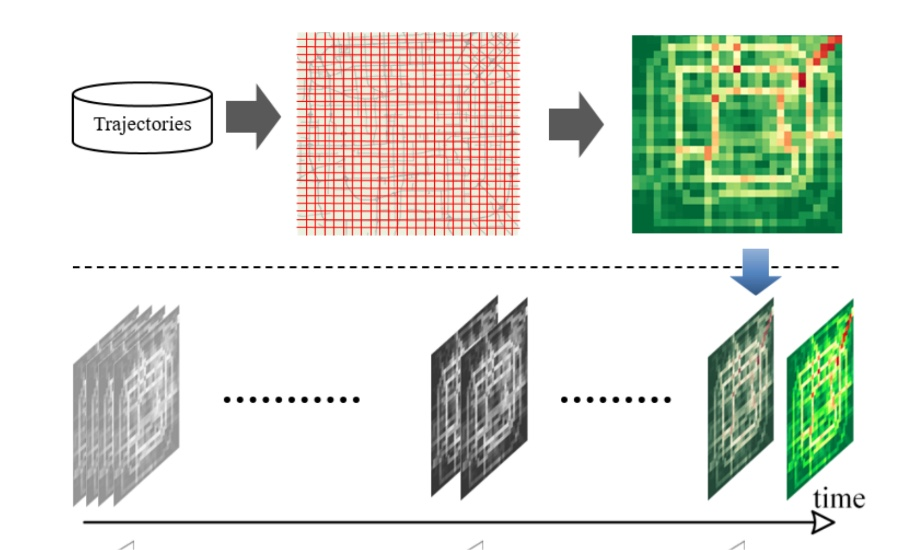
\includegraphics[width = 0.66\textwidth]{video}
%    \vskip 0.2em
%  \wuhao 栅格图中绿色表示该区域上的交通流量较少,红色表示较拥堵。
%    \vspace{0.2em}
%\caption{时空交通流量栅格图 \label{video}}
%\end{figure}

\vspace{1em}
\begin{table}[htbp]
\caption{问题描述中用到的符号定义} \label{tb1}
\vspace{0.5em}\centering\wuhao
\begin{tabular}{ll}
\toprule[1.5pt]
\textbf{符号} & \textbf{定义} \\
\midrule[1pt]
$H$ & 栅格图的高度 \\
$W$ & 栅格图的宽度 \\
$C$ & 栅格图的交通度量数,例如包含出入流量两种度量,则$C=2$ \\
$L$ & 时间范围,以小时为单位,例如$L=24$表示一天 \\
$T$ & 时间范围内的等距时间区间数量,例如$T=48$表示将$L$分成48个时间区间 \\
$\mathcal{X}$ & 样本空间 \\
$X$ & 数据集 \\
$N$ & 样本数量 \\
$x_i$ & 第$i$个样本 \\
$x_i^{obs}$ & 样本$i$的可观测部分 \\
$x_i^{mis}$ & 样本$i$的缺失部分 \\
$\mathcal{M}$ & 掩膜张量空间 \\
$M$ & 掩膜张量,用于标识样本某个位置的值是否缺失 \\
$m$ & 掩膜张量中的元素,取值为0或1 \\
\bottomrule[1.5pt]
\end{tabular}
\end{table}

本文将一个城市根据经纬度划分为一个$H \times W$大小的栅格图,每一个格子都表示一个区域;同时,将一天($L=24$)划分为$T$个时间区间(如$T=48$表示一天有48个时间段,每个区间占半小时),记每日的交通流量为一个数据样本$x \in \mathbb{R}^{C\times T \times H \times W}$。

给定由一些独立同分布的时空交通栅格样本组成的集合$\mathbf{X}=\{x_{i}\}_{i=1}^{N}\in \mathcal{X}^{N}$,其中$\mathcal{X}=\mathbb{R}^{C\times T \times H \times W}$。相应地,定义一个掩膜张量集合$\mathbf{M}=\{m_{i}\}_{i=1}^{N}\in \mathcal{M}^{N}$,其中$\mathcal{M}=\{0,1\}^{C\times T \times H \times W}$,并且如果$x_i[c, t, h, w]$是缺失的,则$m_i[c, t, h, w]=0$;否则$m_i[c, t, h, w]=1$。样本$x_i$中的可观测部分用$x_i^{obs}$表示,缺失部分用$x_i^{mis}$表示。

考虑时间缺失值分布特性的数据填充任务的目标是对于每一个样本$x$,利用观测部分$x^{obs}$的信息填充缺失部分$x^{mis}$,使填充后的值与真实值尽可能地接近。

\section{基于时空注意力机制的变分自编码器填充模型} \label{sec3_3}

\subsection{模型架构}
\begin{figure*}[b]
\vspace{-0.2cm} 
\centerline{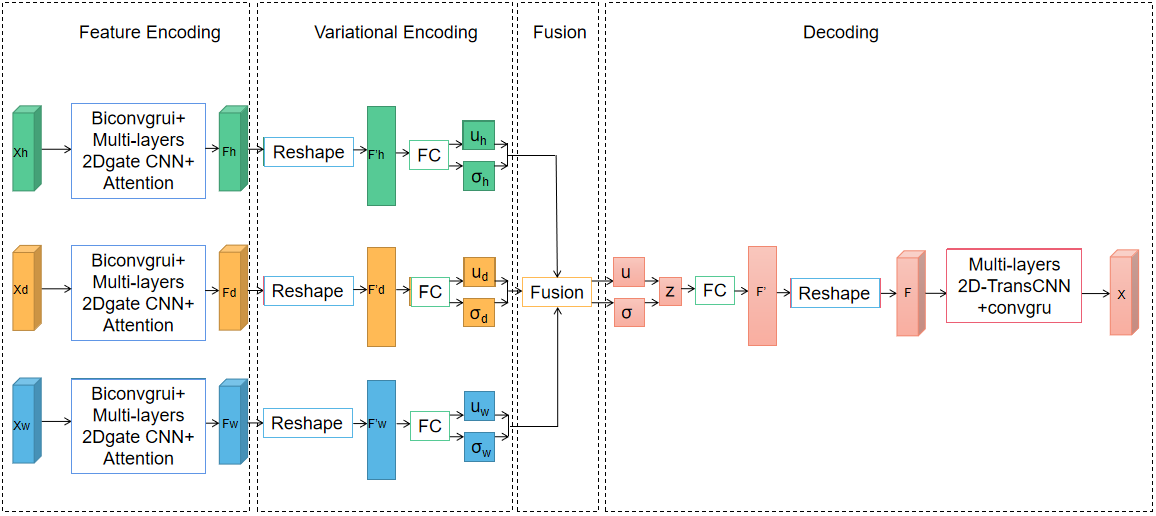
\includegraphics[scale=0.4]{mtsvae.png}}
\caption{多时间流变分自动编码器的整体架构图 \label{MTSVAE}}
\label{fig}
\vspace{-0.2cm} 
\end{figure*}

在本文中,交通数据将被按照不同时间间隔(例如,每小时、每天和每周)划分视频数据研究交通数据填充问题。其中,本文应用了三个时间流数据,包括小时周期、日周期和周周期。每种类型的时间流数据都按照一定的规则进行划分。例如,每小时采样次,取长度为$T_h$, $T_d$ 和 $T_w$的三段,分别作为小时周期、日周期和周周期的输入。因此,可以将小时周期时间流视为张量$x_h \in \mathbb{R}^{C\times T_h\times H\times W}(T_h = \mathcal{P})$,将日周期时间流视为张量$x_d \in \mathbb{R}^{C\times T_d\times H\times W}(T_d = 24\times \mathcal{P})$,将周周期时间流视为张量$x_w \in \mathbb{R}^{C\times T_w\times H\times W}(T_w = 7\times24\times \mathcal{P})$。同时,这些缺失值最初用零填充,这些填充值可以通过\textit{BiConvGRUI}的卷积进行平滑处理。并且填充效果几乎不受此操作的影响\cite{17}。

受\cite{1}的启发,本文提出了一种新颖的基于变分自动编码(\textit{VAE})的多时间流变分自动编码器(\textit{MTSVAE}),用于处理交通数据填充问题。\textit{MTSVAE}可用于学习潜在变量的分布,这个特性帮助其在处理不同缺失率的交通数据时表现强鲁棒性。如图 3-1 所示,多时间流变分自动编码器(\textit{MTSVAE})包含四个关键组件:特征编码、变分编码、融合和解码。特征编码、变分编码和融合用于处理多个时间流数据,而解码用于处理融合数据。

\subsection{特征编码}
\begin{figure*}[htbp]
\vspace{-0.2cm} 
\centerline{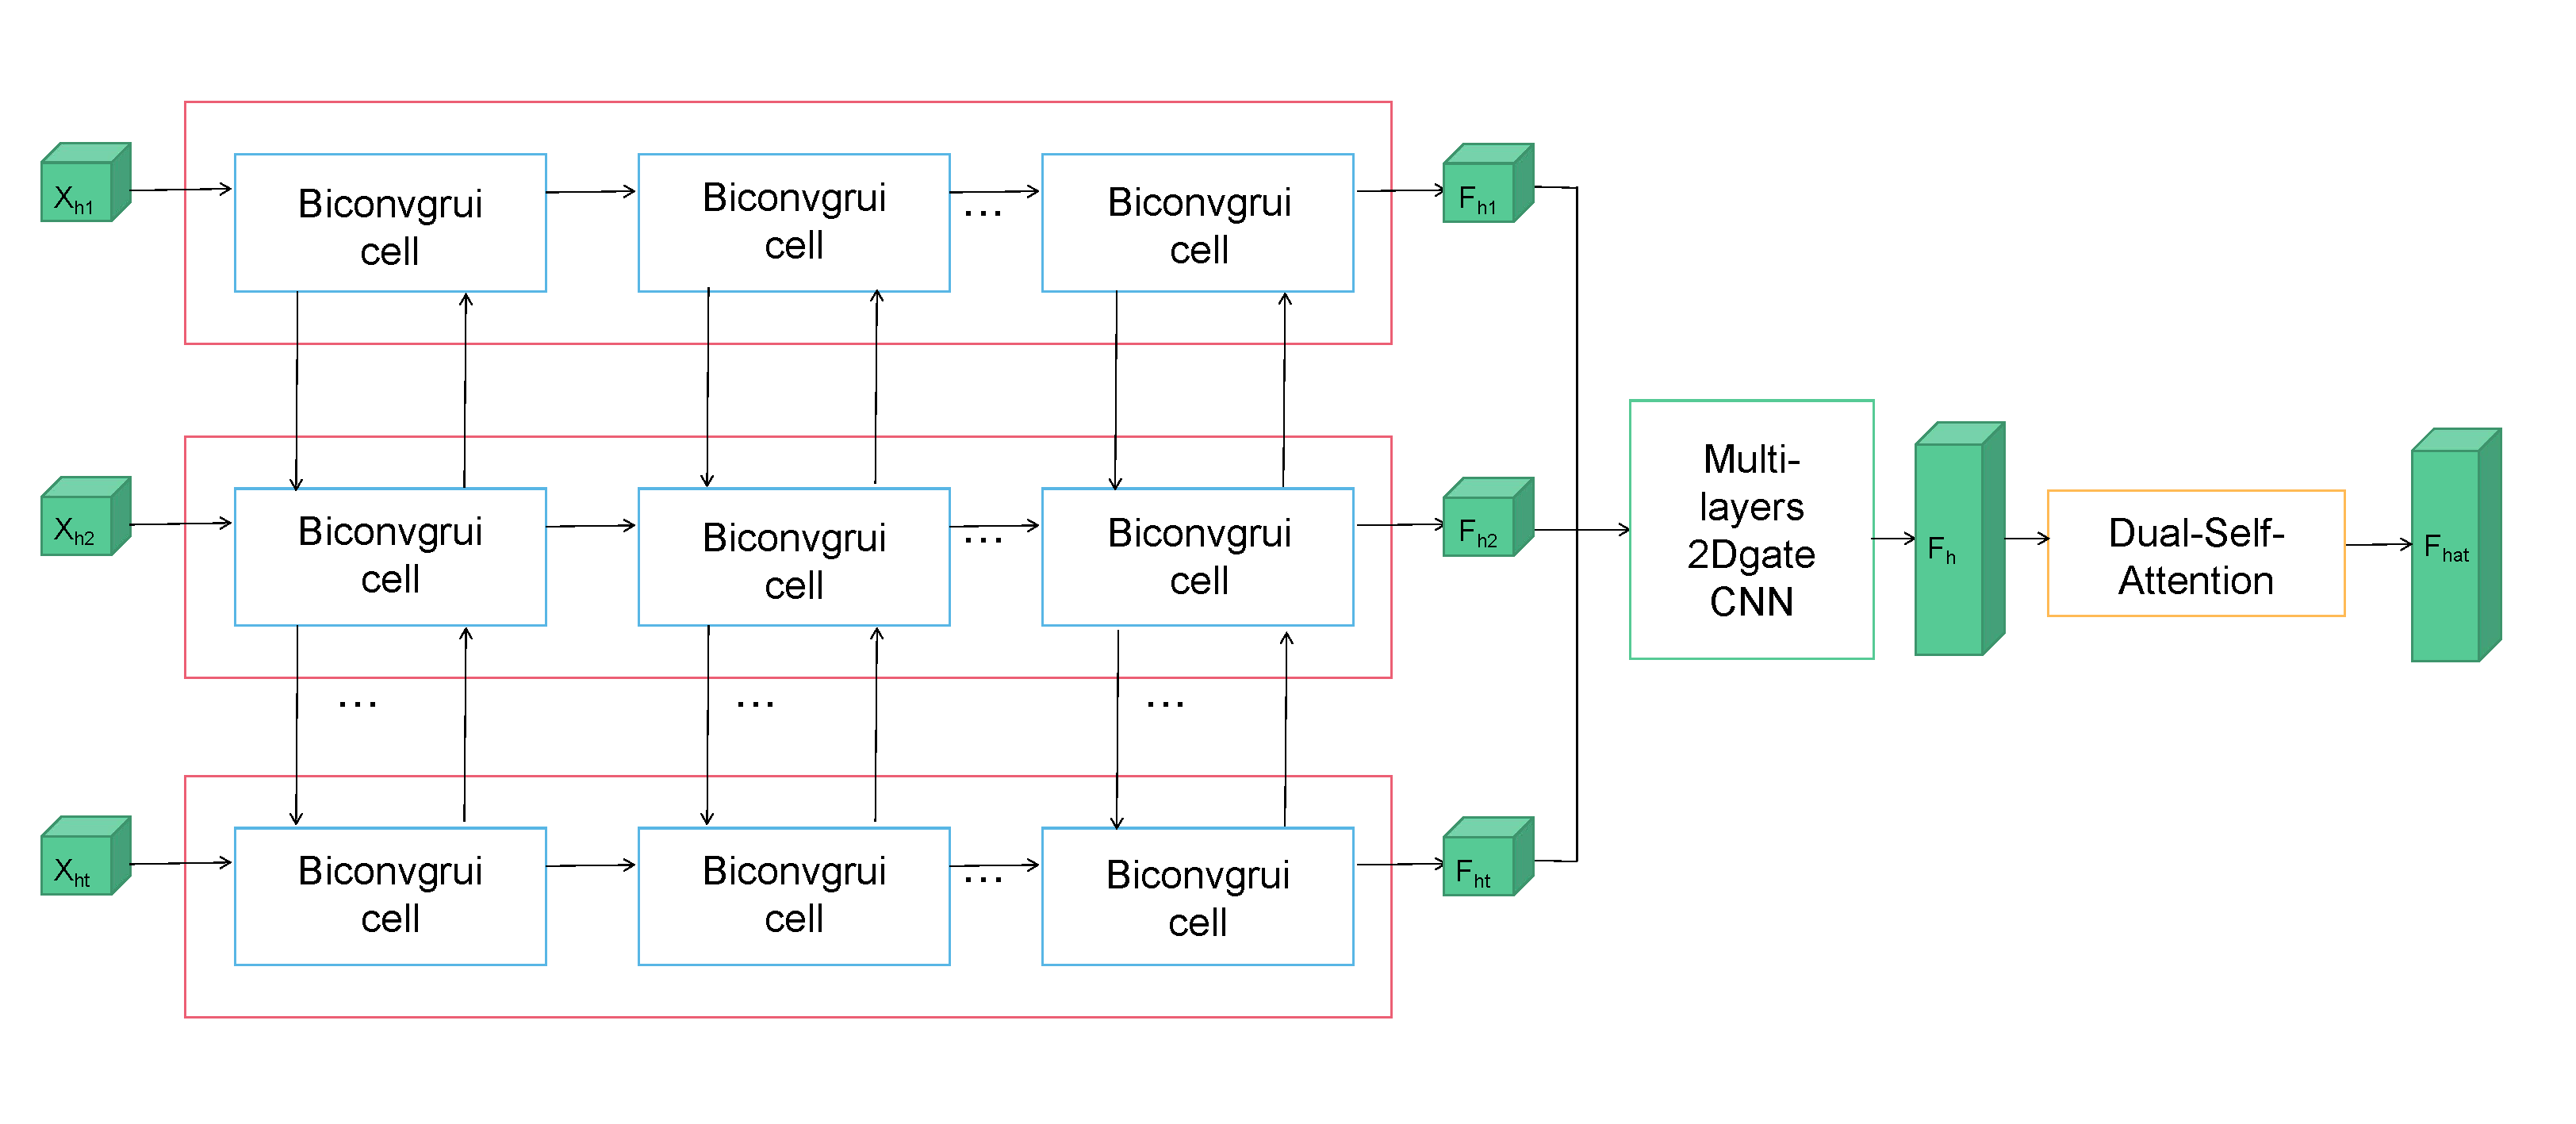
\includegraphics[scale=0.28]{特征编码.pdf}}
\caption{特征编码的整体结构}
\label{fig}
\vspace{-0.2cm}  
\end{figure*}
特征编码模块是\textit{MTSVAE}的一个子模型,它增强了模型捕获不完整数据的时空特征的能力,并使得模型具备区分缺失值与现有值的功能。在特征编码部分中,本章主要设计以下三个模块:1)\textit{BiConvGRUI}模块;2)多层\textit{2D}门控卷积模块;3)双自注意机制模块。如图3-2所示。它们的功能分别是:1)\textit{BiConvGRUI}模块会先刻画带有缺失值的交通数据的时间分布。2)多层\textit{2D}门控卷积被设计来捕获现有值的全局空间特征。3)双自注意机制(由通道自注意力机制和时空自注意力机制组成)被设计以进一步捕捉现有交通数据的动态时空相关性。给定数据$X_d \in \mathbb{R}^{C\times T_d\times H\times W}$作为特征编码的输入,整个特征编码可以用如下公式表示:
\begin{equation}
F_{BI}=B(X_d)
\end{equation}
\begin{equation}
F_{mc}=G(F_{BI})
\end{equation}     
\begin{equation}
F_{att}=M_c(F_{mc})\oplus M_{st}(F_{mc}) 
\end{equation}
其中$F_{BI}\in \mathcal{R}^{C'\times T\times H\times W}$是\textit{BiConvGRUI}的输出特征,$F_{att}\in \mathcal{R}^{C'\times T\times H\times W}$是双自注意力机制的输出特征,$F_{mc}\in \mathcal{R}^{C'\times T\times H\times W}$是多层\textit{2D}门控卷积的输出特征,$\oplus$表示矩阵加法乘积。接下来的内容将分别详细介绍\textit{BiConvGRUI},多层\textit{2D}门控卷积和双自注意力机制。
1)\textit{BiConvGRUI}:\textit{GRUI}在\cite{14}中被提出来并用于多元时间序列的填充问题。\textit{ConvGRUI}\cite{12}与\textit{GRUI}的主要不同是\textit{ConvGRUI}中使用卷积操作替换了\textit{GRUI}中的线性层函数操作,因而\textit{ConvGRUI}适用于处理时空数据。但是,在提取时空数据当前状态的特征时,\textit{ConvGRUI}只关注当前状态之前的时间段信息,而忽略当前状态之后的时间段信息。因此,本章节提出了模型\textit{BiConvGRUI},该模型可以对带有缺失值的交通数据的复杂时间分布进行建模,并捕获当前状态之前和之后的周期信息。与\textit{GRUI}类似,通过提取带有缺失值的交通数据的复杂时间分布特征,\textit{BiConvGRUI}解决了带有缺失值的交通数据的时间特征提取问题。如图3-3所示,\textit{BiConvGRUI}由两个方向相反的\textit{ConvGRUI}组成,分别命名为前向\textit{ConvGRUI}和后向\textit{ConvGRUI}。 
\begin{figure}[htbp]
\vspace{-0.2cm}
\centerline{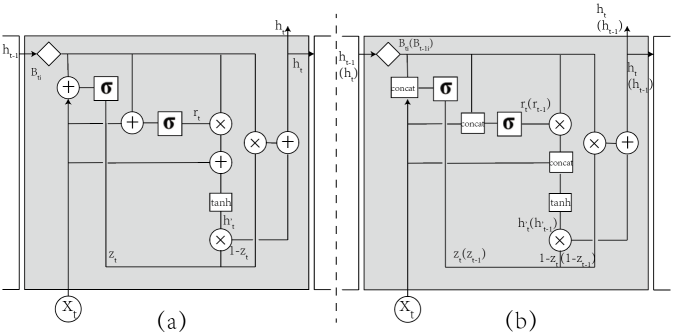
\includegraphics[scale=1.7]{GRUI.png}}
\caption{(a) GRUI和 (b) BiconvGRUI的前向单元(BiconvGRUI的后向单元)}
\label{fig}
\vspace{-0.2cm}
\end{figure}  
 
在\cite{14}中,捕获带有缺失值的数据的时间特征是不容易的。为了捕捉更好的时间特征,本章在模型\textit{BiConvGRUI}中引入了一个新的系数张量$\beta$。系数张量$\beta$可以通过给隐藏状态$h_{t_{i-1}}$中的值进行赋权值,使得模型\textit{BiConvGRUI}处理得到的特征中包含更多的有效特征,进而降低缺失值对于模型\textit{BiConvGRUI}提取时空特征的影响。首先,通过乘以系数张量来更新隐藏状态$h_{t_{i-1}}$:    
\begin{equation}
h'_{pt_{i-1}}={\beta}_{pt_i}\odot h_{pt_{i-1}}
\end{equation}
然后,前向\textit{ConvGRUI}的更新函数为:
\begin{equation}
{\mu}_{pt}={\sigma}(W_{\mu}[h'_{pt_{i-1}},x'_{pt}]+b_{\mu})
\end{equation}
\begin{equation}
r_{pt}={\sigma}(W_r[h'_{pt_{i-1}},x'_{pt}]+b_r)
\end{equation}
\begin{equation}
\tilde{h}_{pt_i}=tanh(W_{\tilde{h}}[r_{pt_i}\odot h'_{pt_{i-1}},x'_{pt}]+b_{\tilde{h}})
\end{equation}
\begin{equation}
{h}_{pt_i}=(1-{\mu}_{pt_i})\odot h'_{pt_{i-1}}+{\mu}\odot \tilde{h}_{pt_i}
\end{equation}
其中$\mu$是更新门系数,$r$是重置门系数,$M_{t_i}$是掩码张量,$\tilde{h}$是候选隐藏状态,$\sigma$是2D卷积函数,[]是拼接操作,$\odot$是逐元素乘法操作,$W_{\mu}$, $W_t$, $W_{\tilde{h}}$, $b_{\mu}$, $b_r$, $b_{\tilde{h}}$和$b_H$是需要训练的参数。后向\textit{ConvGRUI}的更新函数类似于前向\textit{ConvGRUI}的更新函数。而后向\textit{ConvGRUI}被用于提取未来时间的信息。相反,前向\textit{ConvGRUI}被用于提取过去时间的信息。
最后,将前向时间特征$h_{pt_i}$和后向时间特征$h_{ft_i}$融合为时间特征$H_{t_i}$:
\begin{equation}
H_{t_i}=tanh(W_y^{\overset{\rightarrow}{h}}*h_{pt_i}+W_y^{\overset{\leftarrow}{h}}*h_{ft_i}+b_H) 
\end{equation}
其中 ,$W_y^{\overset{\rightarrow}{h}}$, $W_y^{\overset{\leftarrow}{h}}$是训练参数。
在\textit{BiConvGRUI}中,系数张量$\beta$需要找寻到一个适当的权重矩阵,使得隐藏状态的值能够包含更多的有效信息。并且系数张量$\beta$的值需要落在(0, 1)的范围内。参考原论文\cite{14},的计算方式如下:
\begin{equation}
{\beta}_{t_i}=1/e^{[max(0,W_{{\beta}}{\delta}_{t_i}+b_{{\beta}})]}
\end{equation}
其中$W_{{\beta}}$和$b_{{\beta}}$是需要学习的参数。

为了捕捉更好的时间信息,本课题引入了一个可学习的参数${\theta}$(${\theta}$最初设置为0.8),它可以被用来扩展$max(0,W_{{\beta}}{\delta}_{t_i}+b_{{\beta}})$的取值范围,以帮助模型找到更合适的值。前向\textit{ConvGRUI}的计算方式如下:
\begin{equation}
{\beta}_{pt_i}=1/e^{[max(0,W_{{\beta}_p}{\delta}_{pt_i}+b_{{\beta}_p})]^{\theta}}
\end{equation}                                              
此外,使用\textit{ReLU}激活函数计算\textit{max}的结果。后向\textit{ConvGRUI}的计算方式如下:
\begin{equation}
{\beta}_{ft_i}=1/e^{[max(0,W_{{\beta}_f}{\delta}_{ft_i}+b_{{\beta}_f})]^{\theta}}
\end{equation}
为了得到准确的系数张量$\beta$,本章将进一步引入时间滞后张量$\delta$。时滞是指将有用信息从前一时刻传递到当前时刻所需的时间。并且可以通过当前时刻与前一时刻之间的差异来计算时滞。通过记录当前值和最后一个有效值之间的时间滞后值,就可以标记缺失值附近的值,以获得准确的系数张量$\beta$。对于前向\textit{ConvGRUI},我们可以设置当前时刻与前一时刻的差为1。因此,当前一时刻的值存在时,对应的时滞设置为1。当前一个时刻的值丢失时,就没有从前一个时刻传递到当前时刻的任何有效信息。然后,将这个时滞的值设置为前一个时滞的值加 1(即当前时刻与前一时刻的差值)。因此,前向\textit{ConvGRUI}的时滞张量计算公式如下: 
\begin{equation}
{\delta}_{pt_i}^{c\times h\times w}=\begin{cases}
1,&\mathcal{M}_{pt_{i-1}}^{c\times h\times w}==1\\
{\delta}_{pt_{i-1}}^{c\times h\times w}+1,&\mathcal{M}_{pt_{i-1}}^{c\times h\times w}==0 and i>0\\
0,&i==0
\end{cases}
\end{equation}
其中,$pt_i$, $pt_{i-1}$分别代表相邻的两个时间点,$\mathcal{M}_{pt_{i-1}}^{c\times h\times w}$表示在时间点坐标 (c,h,w) 对应的值是否缺失,缺失时为0,否则为1。
对于后向的\textit{ConvGRUI},本课题将当前时刻与上一个时刻的差值设置为 -1。而后向\textit{ConvGRUI}的时滞张量计算公式如下:
\begin{equation}
{\delta}_{ft_i}^{c\times h\times w}=\begin{cases}
-1,&\mathcal{M}_{ft_{i-1}}^{c\times h\times w}==1\\
{\delta}_{ft_{i-1}}^{c\times h\times w}-1,&\mathcal{M}_{ft_{i-1}}^{c\times h\times w}==0 and i>0\\
0,&i==0
\end{cases}
\end{equation}
其中,$ft_i$, $ft_{i-1}$分别代表相邻的两个时间点。
在栅格地图的区域中,观察到的时间序列作为样本给出:
\begin{equation}
X= \begin{bmatrix}
none & 9 & none & 4\\
2 & none & 5 & none\\
3 & none & none & 9\nonumber
\end{bmatrix}
T= \begin{bmatrix}
0\\
1\\
2\nonumber
\end{bmatrix}
\end{equation}
其中“none”是缺失值。根据公式(2-13)和(2-14),可以得到两个时滞张量:
\begin{equation}
{\delta}_{pt_i}= \begin{bmatrix}
0 & 0 & 0 & 0\\
1 & 1 & 1 & 1\\
1 & 2 & 1 & 2\nonumber
\end{bmatrix}
{\delta}_{ft_i}= \begin{bmatrix}
0 & 0 & 0 & 0\\
-1 & -1 & -1 & -1\\
-1 & -2 & -1 & -2\nonumber
\end{bmatrix}
\end{equation}
2)多层 \textit{2D} 门控卷积:在\cite{10}中,\textit{2D}门控卷积由于在普通卷积的基础上加入了门机制,使得相比起普通卷积,它更适用于图像修复问题。在本章中,\textit{2D}门控卷积将被用于交通数据填充问题。同时,由于\textit{2D}门控卷积较好的提取空间特征的性能,可以显著增强模型提取空间特征的能力。与\textit{2D}卷积类似,由于卷积核大小的限制,会限制模型卷积的范围。因此,在编码模块中堆叠了多个\textit{2D}门控卷积,命名为多层\textit{2D}门控卷积,以扩大卷积的范围,从而使得模型可以学习全局特征。在每个时间间隔中,\textit{2D}门控卷积最初检测哪些像素包含无效消息(即先前缺失的部分),并更加关注有效消息以学习重要特征。

3)双自注意力机制:双注意力机制\cite{15}被提出用于场景分割。然而,原始双注意力机制只关注空间数据。在本章中,使用在双注意力机制基础上扩展的双自注意力机制机制来处理时空问题。它由通道自注意力机制和时空自注意力机制组成,如图3-4和图3-5所示。而且时空自注意力和通道自注意力从输入特征中并行学习目标的相关特征。最后将它们各自的输出相加作为最终输出。具体说明如下:

时空自注意力机制。与双注意力机制的空间自注意力不同,时空自注意力机制可以处理时空数据。把特征$F_{mc}\in \mathbb{R}^{C'\times T\times H\times W}$作为时空自注意力的输入。首先,特征经过卷积操作和重构操作可以得到特征图$F’_{mc}\in \mathbb{R}^{C'\times N}$。然后,将特征$F’_{mc}$同$F’_{mc}$的转置进行乘积操作,经过softmax激活函数的操作,生成权重分布矩阵$F''_{mc}\in \mathbb{R}^{N\times N}$。最后将特征$F’_{mc}$与权重分布矩阵$F''_{mc}$相乘,并将输出重塑为与特征$F_{mc}$相同的形状,这样就可以将多个特征相加生成特征$F_{st}$。
\begin{figure}[htbp]
\centerline{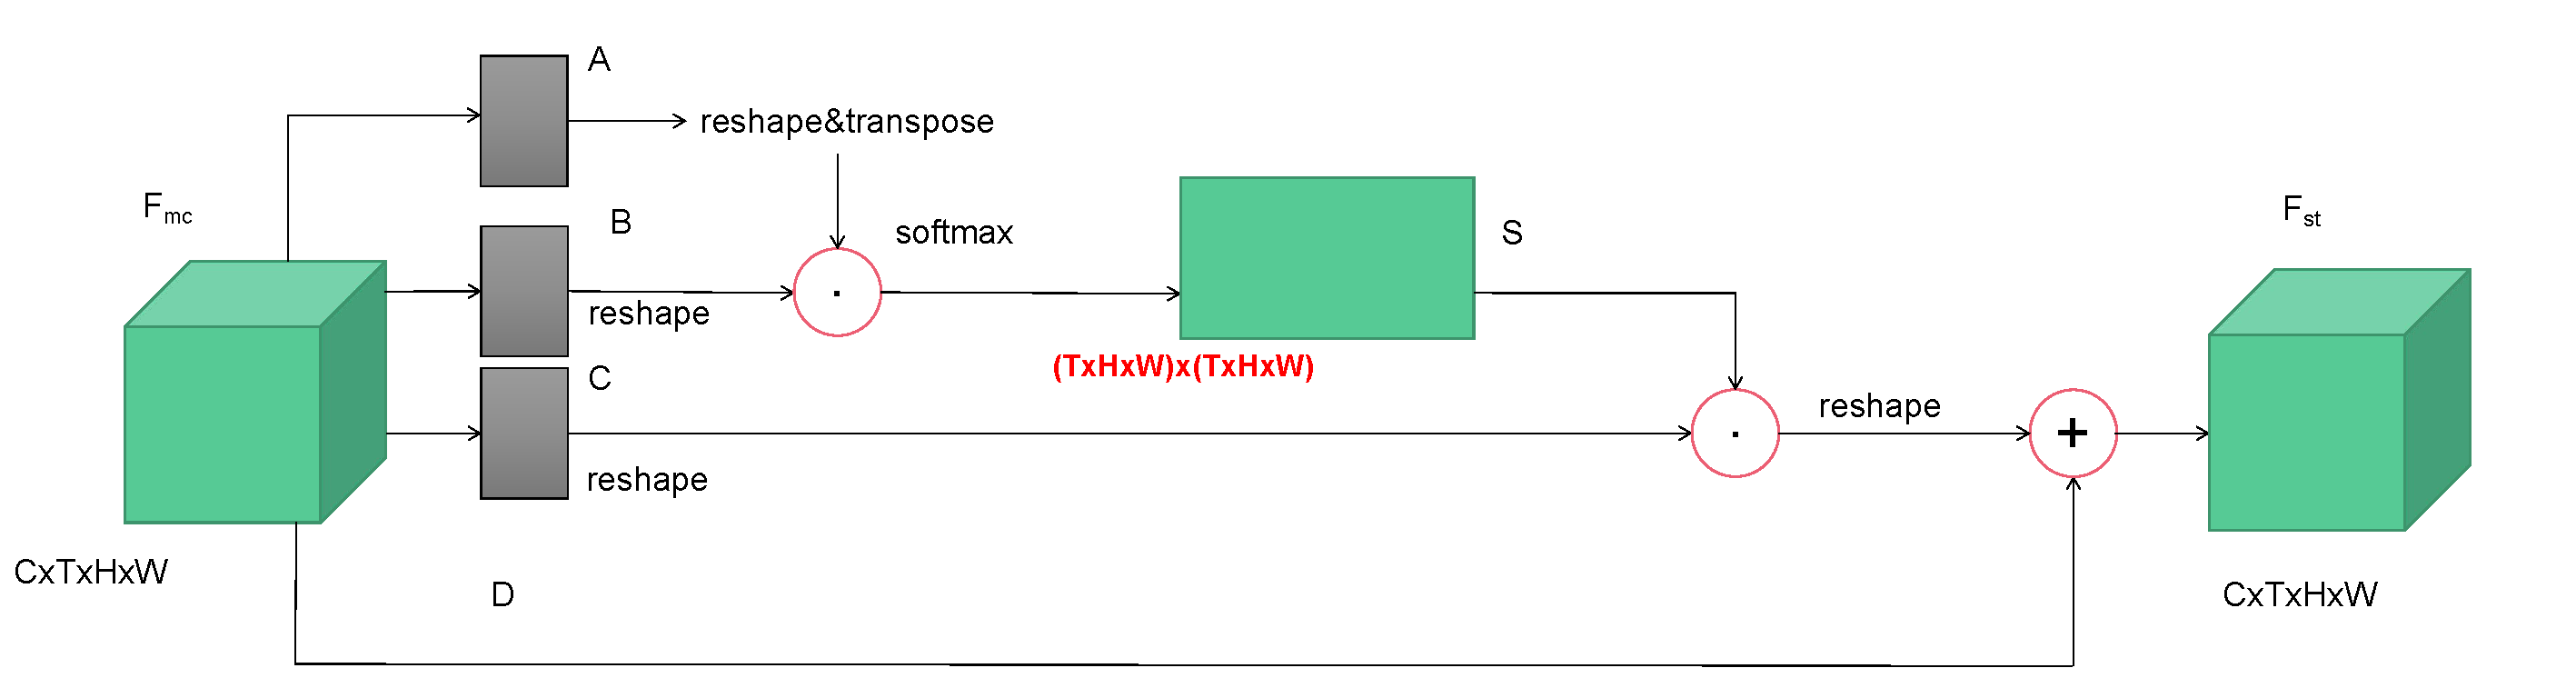
\includegraphics[scale=0.3]{时空自注意力整体结构.pdf}}
\caption{时空自注意力整体结构}
\label{fig}
\end{figure}

通道自注意力机制。在双自注意力机制中,还有一个重要的组成构建-通道自注意力。通道自注意力机制通常被用来学习交通数据的流入和流出的相关性。把特征$F_{mc}\in \mathbb{R}^{C'\times T\times H\times W}$作为通道自注意力的输入。首先,特征$F’_{mc}\in \mathbb{R}^{C'\times N}$经过重塑操作,可以得到三个特征图$F’_{mc}\in \mathbb{R}^{C'\times N}$。然后,将特征$F'_{mc}$乘以$F’_{mc}$的转置,得到的结果通过softmax激活函数的操作生成权重分布矩阵$F''_{mc}\in \mathbb{R}^{C'\times C'}$。最后将特征$F’_{mc}$与权重分布矩阵$F''_{mc}$相乘,并将输出重塑为与特征$F_{mc}$相同的形状,这样就可以将特征$F_{mc}$相加生成特征$F_{st}$。
\begin{figure}[htbp]
\vspace{-0.2cm}
\centerline{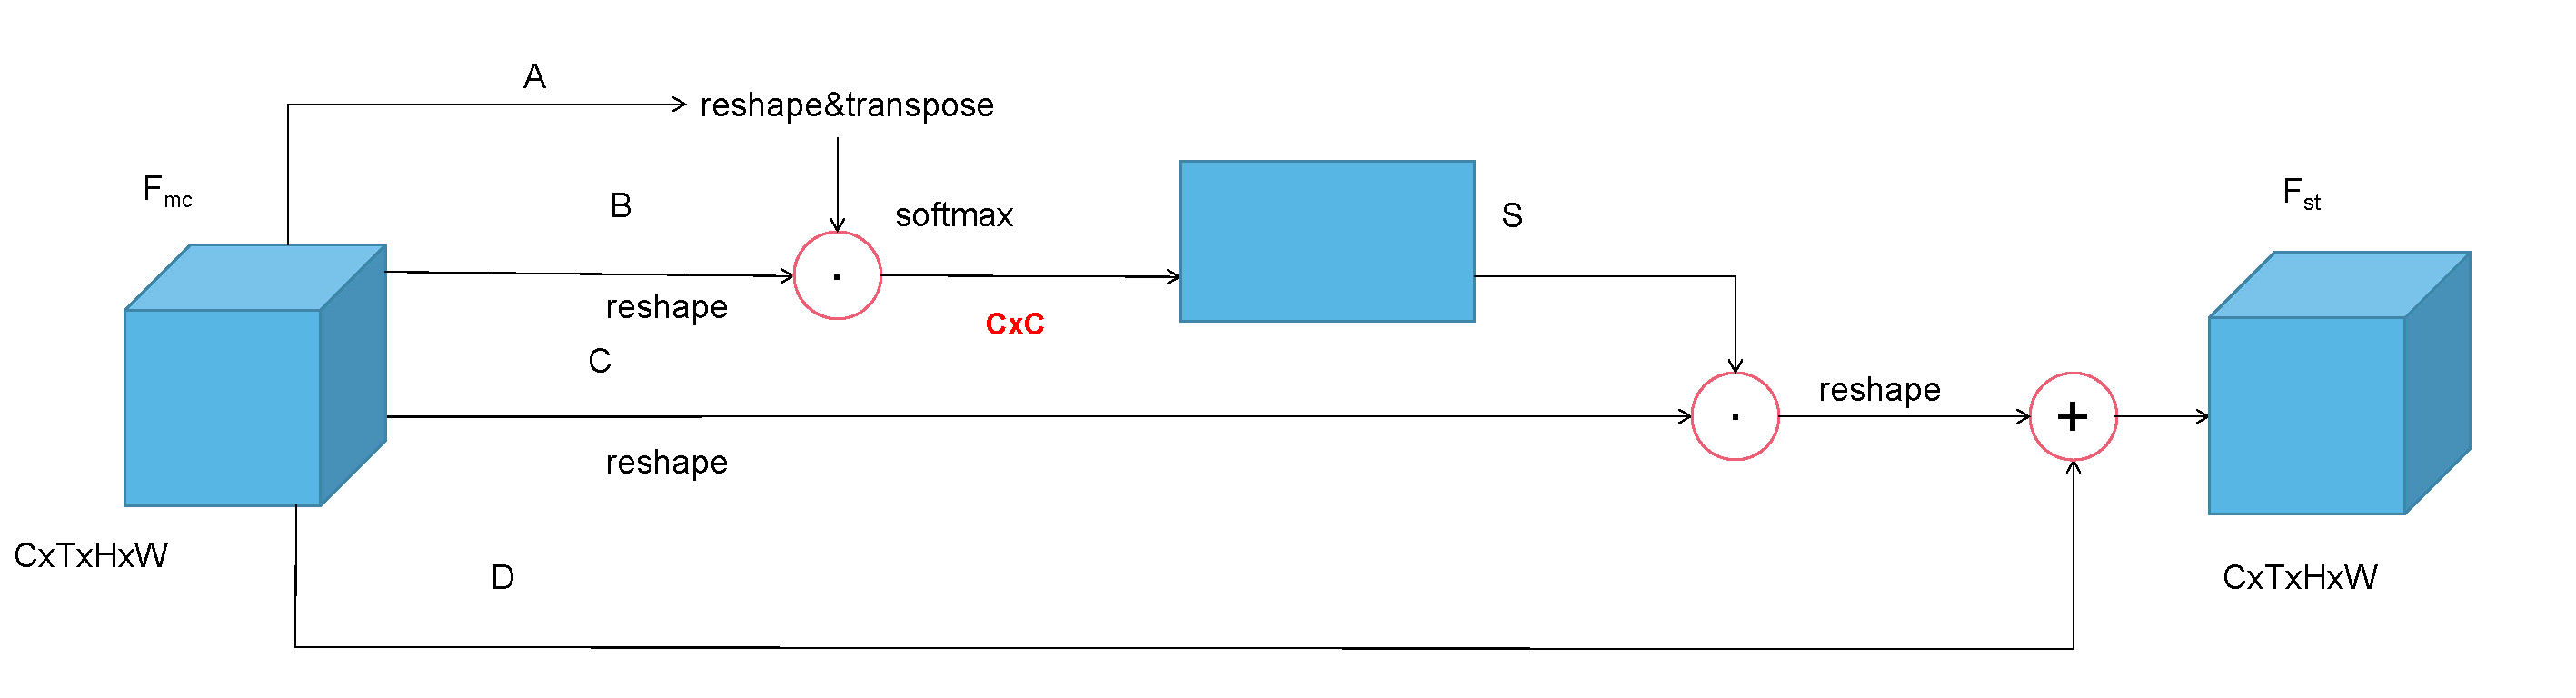
\includegraphics[scale=0.3]{通道自注意力整体结构.pdf}}
\caption{通道自注意力整体结构}
\label{fig}
\vspace{-0.2cm}
\end{figure}

最后将$F_{st}$和$F_{c}$求和为$F_{att}\in \mathbb{R}^{C'\times T\times H\times W}$,如上式(3-3)所示。

\subsection{变分编码}
模型的鲁棒性是衡量模型在存在外界干扰的情况下的性能。这意味着,如果模型的鲁棒性越强,那么它抗干扰的能力也就越强。而在本文中,定义的外界干扰主要是指交通数据中存在的缺失值。因而,如何使模型呈现更好的鲁棒性,抵御这种外界干扰,是一个很重要的问题。在VAE\cite{18}算法中,通过在编码过程中引入高斯噪声,可以提高模型的鲁棒性。这种编码过程被称为变分编码。同时,引入高斯噪声可以帮助模型捕获更多有效信息。受此启发,本章决定应用变分编码来增强模型的鲁棒性。在变分编码过程中,输入经过扁平层和线性层的处理,生成初始潜变量$z$的参数化均值$\mu$和对数偏差$log{\sigma}^2$。接下来,可以通过重新参数化技巧\cite{16}生成$z$,如下所示:

\begin{equation}
z=\mu+\sigma\oplus\varepsilon
\end{equation}  
其中${\mu}$是从$\mathit{N}(0,1)$中采样的, $\oplus$是矩阵加法。
\subsection{融合}
在融合模块中,三个相互独立的分布函数可以通过加权融合形成一个新的分布函数。$\mu$和$\sigma$可以分别表示为:
\begin{equation}
{\mu}_k=w_h\otimes {\mu}_h+w_d\otimes {\mu}_d+w_w\otimes {\mu}_w
\end{equation}
\begin{equation}
{\sigma}_k^2=w_h\otimes {\sigma}_h^2+w_d\otimes {\sigma}_d^2+w_w\otimes {\sigma}_w^2
\end{equation}
其中,$w_h$, $w_d$, $w_w$是需要在训练过程中学习的参数,数值表示每个独立时间分量对最终结果的影响程度。$\otimes$是\textit{Hadamard}乘积。
\subsection{解码}
解码模块用于重构样本。其中解码模块由四个部分组成,分别称为压缩层、重塑层、多层2D反卷积和convGRU。其中,多层2D反卷积用于重构空间信息,convGRU用于重构时间信息。给定融合模块的输出作为解码模块的输入,使用压缩层和重塑层从融合的潜在变量中重构时空特征。然后,重建的时空特征被输入到多层2D反卷积中进行处理,再将处理结果通过convGRU重建完整的交通数据$X_k$。用公式(3-19)训练$X_k$。在损失函数收敛到最优解后,应用$X_k$的值来替换$X$的缺失值,如下所示:

\begin{equation}
X_{imputation}=M\odot X+(1-M)\odot X_k
\end{equation}

\section{模型训练}
在普通的VAE的损失函数基础上,将KL损失函数中的普通高斯分布替换为融合高斯分布,得到MTSVAE的损失函数,结果如式(3-19)所示。  
\begin{align}
&\mathcal{F}=\sum_{i=1}^{T}m_i\otimes||x_i-\bar{x}_i||_F\\
&+\beta\sum_{i=1}^{T}KL \Big(N(w_{hi}\otimes{\mu}_{hi}+w_{di}\otimes{\mu}_{di}+w_{wi}\otimes{\mu}_{wi},\nonumber\\
&w_{hi}\otimes{\sigma}_{hi}^2+w_{di}\otimes{\sigma}_{di}^2+w_{wi}\otimes{\sigma}_{wi}^2)||N(0,1) \Big)\nonumber
\end{align}
式(3-19)中,$\beta$为超参数,用于平衡两部分的损失,$\otimes$为Hadamard乘积。由于缺乏完整的数据集,第一项需要计算为$m_i\otimes||x_i-\bar{x}_i||_F$,表示观察部分$x_i^{obs}$的重建误差。最后一项是两个分布之间的\textit{Kullback-Leibler}距离。(即潜在变量的分布$N(w_{hi}\otimes{\mu}_{hi}+w_{di}\otimes{\mu}_{di}+w_{wi}\otimes{\mu}_{wi},w_{hi}\otimes{\sigma}_{hi}^2+w_{di}\otimes{\sigma}_{di}^2+w_{wi}\otimes{\sigma}_{wi}^2)$和目标分布$N(0,1)$)。
\begin{figure}[htbp] 
\centering
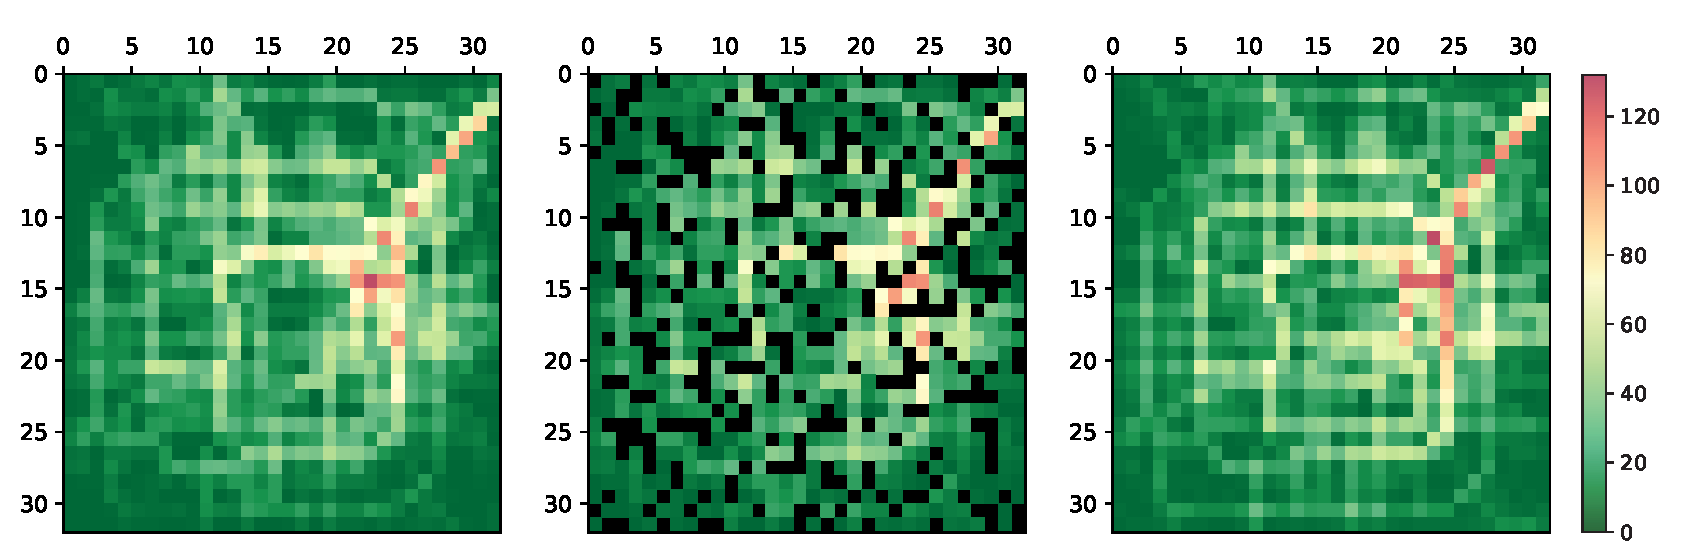
\includegraphics[width=\textwidth]{impute.eps}
\vspace{-1em}
\caption{填充效果图 \label{impute}}
\end{figure}
\section{模型推断}
一旦模型训练完毕, MSTVAE 可以被用于重构缺失值, 公式如下所示:
\begin{equation}
p(x^{mis}|x^{obs}) = \int p_{\theta}(x^{mis}|z_{K})q_{\phi}(z_{K}|x^{obs}) dz_{K},	
\end{equation}

即可以在给定数据的观测值的条件下推断出其缺失部分,其中最主要的就是借助隐变量作为推断的桥梁。本文选取了TaxiBJ数据集中某一时刻的交通梜格数据作为填充效果的展示,如图3-7所示,绿色表示该区域上的交通人流量较少,红色表示人流量较多。左边的图表示真实的栅格数据,中间的图由真实数据根据MCAR模式随机缺失产生,右边的图为缺失数据经过本文模型处理后得到的完整数据。左右两幅图差异越小表明模型填充效果越好。

\section{实验与分析}
本小节首先介绍了实验所用的数据集,然后列出了实验环境和模型参数的设置,接着进行了对比实验和模型复杂度的分析,最后给出了消融实验的结果。
\subsection{数据集}
为了定量地评价所提出的模型的填充效果,本文在如下三个开源的交通轨迹数据集上做了对比实验,分别为TaxiBJ\cite{zhang2017deep}、TaxiNYC\cite{illinoisdatabankIDB-9610843}、BikeNYC\cite{zhang2017deep},数据集概况如表\ref{tb_dataset}所示。

(1)\textbf{TaxiBJ:}该数据集为北京市内所有出租车GPS轨迹数据,分别从四个时间段进行记录:2013年7月1日至2013年10月30日、2014年3月1日至2014年6月30日、2015年3月1日至2015年6月30日、2015年11月1日至2016年4月10日。

(2)\textbf{TaxiNYC:}该数据集包含了从2010年到2013年间纽约市的出租车GPS记录,其中有近70亿条出租车接送客轨迹数据,每个记录包括了接送客的具体时间戳、位置坐标和行驶距离。

(3)\textbf{BikeNYC:}该数据集来自纽约市自行车租赁系统,日期从2014年4月1日至2014年9月30日。每一条轨迹数据包括租赁开始时间戳、结束时间戳、租赁时长、起始租赁点和归还点ID。

以上轨迹数据均可通过定义(\ref{def_flow})转换为交通出入流量数据。本文按照五个缺失值比例10\%,30\%,50\%,70\%,90\%随机手动生成相应的数据集,接着使用归一化将数据集数值范围缩放到区间[-1,1]内。对于每个数据集,本文将数据集前90\%的样本作为训练集,剩余的样本作为测试集,又取训练集中的90\%作为验证集。为了防止模型训练产生过拟合现象,我们保存在验证集上损失函数最小的模型参数用于测试。


\begin{table}[htbp] 
\renewcommand\arraystretch{1.2}
\caption{数据集描述} \label{tb_dataset}
\vspace{0.5em}\centering\wuhao
\begin{tabular*}{\hsize}{@{}@{\extracolsep{\fill}}cccc@{}}
\toprule[1.5pt]
数据集 & TaxiBJ\cite{zhang2017deep} & TaxiNYC\cite{illinoisdatabankIDB-9610843} & BikeNYC\cite{zhang2017deep} \\
\midrule[1pt]
数据类型 & 出租车GPS        & 出租车GPS         & 自行车租赁 \\ 
采集地点 & 北京 & 纽约 & 纽约\\
时间范围 & \makecell[c]{7/1/2013 $\sim$ 10/30/2013\\3/1/2014 $\sim$ 6/30/2014\\3/1/2015 $\sim$ 6/30/2015\\11/1/2015 $\sim$ 4/10/2016} & \makecell[c]{1/1/2010 $\sim$ 12/31/2010\\1/1/2012 $\sim$ 12/31/2013} & \makecell[c]{4/1/2014 $\sim$ 9/30/2014} \\ 
时间区间 & 30 分钟      & 1 小时   & 1 小时 \\
栅格图尺寸   & (32, 32)        & (10, 20)         & (16, 8) \\
时间区间数 & \num[group-separator={,}]{22459}   & \num[group-separator={,}]{26304}          & 4392 \\
\bottomrule[1.5pt]
\end{tabular*}
\end{table}

\subsection{实验设置}
(1)\textbf{实验环境}:本章实验均在GPU服务器上完成,表\ref{env1}给出了实验所采用的软硬件环境的具体细节。
\begin{table}[htbp] 
\caption{实验软硬件环境} \label{env1}
\vspace{0.5em}\centering\wuhao
\begin{tabular}{cc}
\toprule[1.5pt]
环境 & 参数 \\
\midrule[1pt]
操作系统 & Ubuntu 20.04.2.0 LTS \\
内存 & 128GB \\
磁盘 & 1TB SSD \\
处理器 & 英特尔至强Gold 5218R@2.10GHz \\
图形卡 & GeForce RTX 3080 \\
CUDA版本 & 11.1 \\
开发语言 & Python 3.8 \\
深度学习框架 & Pytorch 1.8.1 \\
\bottomrule[1.5pt]
\end{tabular}
\end{table}

(2)\textbf{模型超参设置}:在BiconvGRUI模块中,我们将内核大小调整为3,步幅调为2,输出通道数调整为16。BiconvGRUI单元格的数量被设置为6(小时流)、24(每日流)和48(周流)。对于每个二维卷积模块,内核大小被调整为3,步幅被调整为2。每个二维卷积的输出通道数按升序依次为32、64和128。在congGRU模块中,我们将内核大小调整为3,步幅调为2,输出通道数调整为2。我们根据经验设置convGRU细胞的数量为24个。利用Adam优化器进行梯度下降,初始学习速率设置为$10^{-3}$。此外,我们还将TaxiNYC、TaxiBJ和BikeNYC的epoch总数分别设置为200、500和2000。

(3)\textbf{评价指标}:为了定量评估本章节的方法和基线方法,通过归一化均方误差(\textit{NMSE})和均方根误差(\textit{RMSE})来衡量真实数据和估算数据的适用性,其定义为
\begin{equation}
NMSE=\frac{1}{t}*\frac{\sum_{j=1}^J\sum_{k=1}^K[(1-M)\otimes(x-\bar{x})]^2}{\sum_{j=1}^J\sum_{k=1}^K[(1-M)\otimes x]^2}
\end{equation}
\begin{equation}
RMSE=\sqrt{\frac{1}{t}*{\sum_{j=1}^J\sum_{k=1}^K[(1-M)\otimes(x-\bar{x})]^2}}
\end{equation}

\subsection{对比实验结果与分析}
在本节中,将模型MTSVAE与九种基线方法进行比较:ARIMA\cite{3}、knn\cite{19}、HaLRTC\cite{4}、ConvLSTM\cite{20}、DeepSTNPlus\cite{5}、CombCN\cite{21}和 ST-VAE\cite{8}。

图3-7至图3-9显示了MTSVAE和其他基线模型在三个不同缺失率数据集上的RMSE和NMSE的比较结果。本章提出的模型MTSVAE在不同缺失率的数据集中都得到最低的RMSE和NMSE,这表明,模型MTSVAE具有较强的鲁棒性,因而相比其它模型,它更适用于处理交通数据的填充问题。

\begin{figure}[htbp] 
\centering
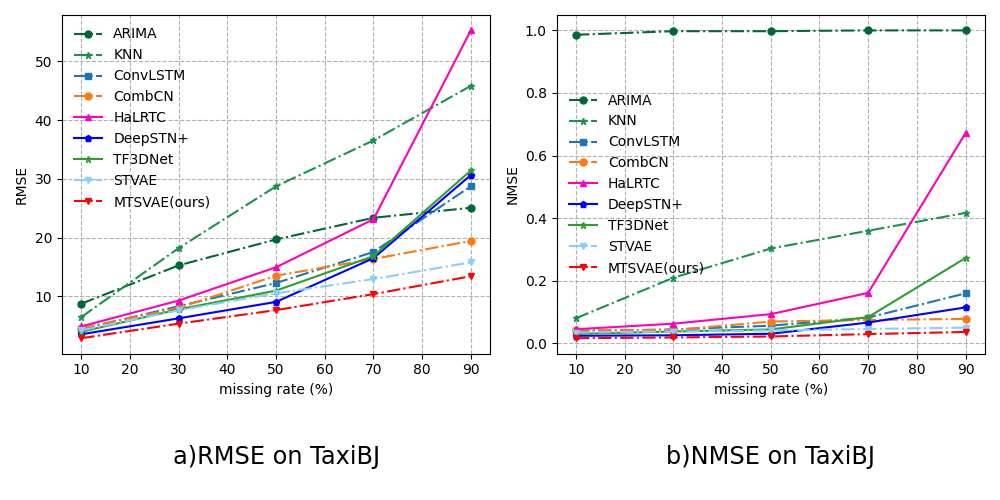
\includegraphics[width=\textwidth]{myplot_taxibj.png}
\vspace{-1em}
\caption{填充效果图 \label{impute}}
\end{figure}

对于传统方法(Auto-Regressive Integrated Moving Average(ARIMA)和 k-NearestNeighbor(KNN)),ARIMA主要关注预测值的历史记录,即时间特征,而忽略了空间特征。相比之下,knn主要关注于空间特征,而忽略了时间特征。对于基于张量的方法(HaLRTC),它同时使用了时间特征和空间特征。因此,由图3-8和图3-9可以发现,HaLRTC应用在缺失率较低的TaxiNYC和BikeNYC两个数据集上时,其表现结果都优于ARIMA和KNN。但它只利用了短期历史特征和局部空间特征,而忽略了长期历史特征和全局空间特征,限制了HaLRTC在TaxiBJ数据集中的结果。相比之下,MTSVAE可以学习长期的时间特征和全局空间特征,这使得它在所有数据集中都优于上述模型。

\begin{figure}[htbp] 
\centering
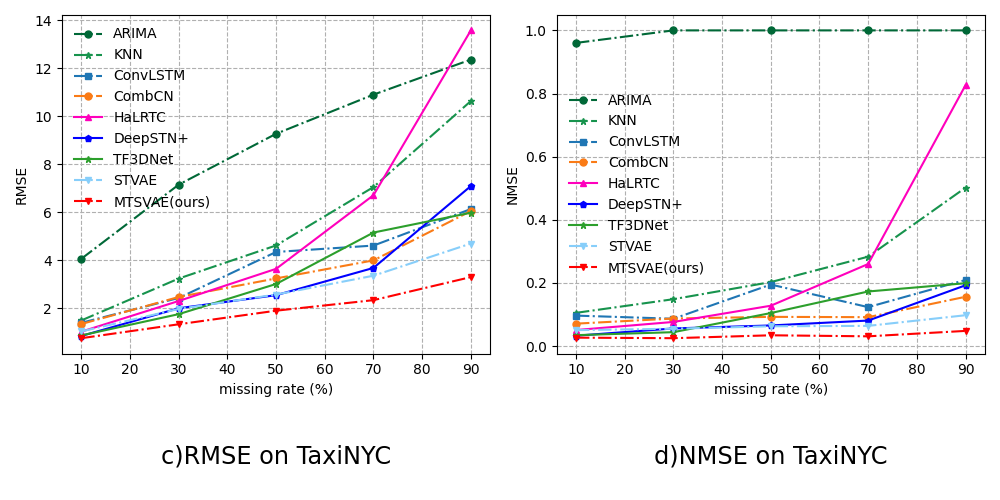
\includegraphics[width=\textwidth]{myplot_taxinyc.png}
\vspace{-1em}
\caption{填充效果图 \label{impute}}
\end{figure}

对于基于神经网络的方法,有ConvLSTM、DeepSTNPlus、CombCN和ST-VAE。前两个模型应用于交通数据的预测问题,其余模型用于交通数据的填充问题。在应用于交通数据预测问题的模型中,ConvLSTM将卷积操作集成到LSTM单元,使得它不仅能处理短期时间特征,还能处理长期时间特征,因而使它的性能优于HaLRTC。但遗憾的是,ConvLSTM模型仍然忽略了对全局特征的应用,这是限制它的实验效果进一步提升的一个重要因素。相比之下,MTSVAE可以捕获不完整交通数据的全局空间特征。

\begin{figure}[htbp] 
\centering
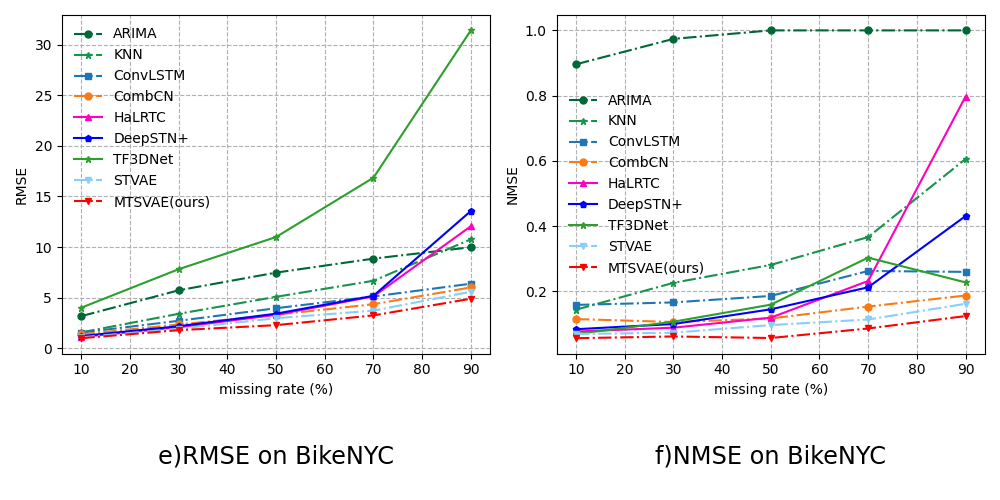
\includegraphics[width=\textwidth]{myplot_bikenyc.png}
\vspace{-1em}
\caption{填充效果图 \label{impute}}
\end{figure}

DeepSTNPlus是一个基于自动编码器的交通预测模型。DeepSTNPlus的两个重要组成构件是多层空间卷积模块,以及时间卷积模块。多层空间卷积模块可以帮助模型学习全局空间特征。时间卷积模块可以帮助模型学习时间特征。但是,DeepSTNPlus模型有一个很重要的缺陷就是,模型训练需要使用不带缺失值的训练数据集。相比之下,MTSVAE中的特征编码模块可以处理不完整的数据,这意味着可以通过使用不完整的交通数据训练模型MTSVAE。

在应用于交通数据填充问题的模型中,CombCN是基于自动编码器的模型,主要包含了3D卷积以及2D卷积。它使用3D卷积处理时间一致性问题,以及使用2D卷积提取空间特征。这些特点使得它可以有效处理视频填充问题。相比之下,MTSVAE使用BiconvGRUI提取有效时间特征,以及采用2D门控卷积学习有效空间特征。同时,MTSVAE是基于变分自编码器的模型,这意味着MTSVAE比那些基于自编码器的模型具有更强的鲁棒性。因此,MTSVAE比CombCN表现得更出色。

ST-VAE是一种类似的深度贝叶斯模型,它可以通过西尔维斯特标准化流变分编码提取不完整数据和潜在变量之间的随机映射。同时,它还可以通过3D卷积来学习时空特征。但遗憾的是,它忽略了不同的时间依赖关系的特性。相比之下,我们提出的模型MTSVAE可以学习不同时间依赖性的特征,这使得其性能优于ST-VAE。

\begin{table}[htbp] 
\caption{消融实验对比表(Mts:Multi temporal streams,FEm:Feature Encoding module)} 
\label{tb_ab} 
\vspace{0.5em}\centering\wuhao
\subtable[TaxiBJ数据集的RMSE / NMSE指标对比]{
\begin{tabular*}{\hsize}{@{}@{\extracolsep{\fill}}lccccc@{}}
%\begin{tabular}{lccccc}
\toprule[1.5pt]
缺失率 & 10\% & 30\% & 50\% & 70\% & 90\%\\
\midrule[1pt]
Single stream VAE         & 3.86/0.0280  & 7.15/0.0371  & 10.67/0.0417  & 12.44/0.0453  & 15.05/0.0449 \\
\textit{MTSVAE} w/o Mts  & 3.10/0.0183  & 5.92/0.0220  & 8.28/0.0253  & 10.41/0.0302  & 14.27/0.0379 \\
\textit{MTSVAE} w/o FEm   & 3.80/0.0278  & 7.00/0.0310  & 10.18/0.0382  & 12.77/0.0439  & 14.84/0.0428 \\
\textit{MTSVAE}           & \textbf{2.90}/\textbf{0.0160}  & \textbf{5.38}/\textbf{0.0183}  & \textbf{7.68}/\textbf{0.0215}  & \textbf{10.40}/\textbf{0.0290}  & \textbf{13.44}/\textbf{0.0359} \\
\bottomrule[1.5pt]
\end{tabular*}
}


%\subtable[TaxiNYC数据集下的消融实验对比表]{
%\begin{tabular}{ccccccccccc}
%\toprule[1.5pt]
%缺失率 &\multicolumn{2}{c}{10\%} & \multicolumn{2}{c}{30\%} & \multicolumn{2}{c}{50\%} & \multicolumn{2}{c}{70\%} & \multicolumn{2}{c}{90\%}\\
%& NMSE & RMSE & NMSE & RMSE & NMSE & RMSE & NMSE & RMSE & NMSE & RMSE \\
%\midrule[1pt]
%Pure-3DVAE      & 0.0358 (0.0002) & 4.34 (0.01) & 0.0406 (0.0003) & 8.01 (0.03)  & 0.0454 (0.0007) & 11.12 (0.08) & 0.0497 (0.0008) & 13.57 (0.10) & 0.0710 (0.0014) & 18.85 (0.18)\\
%STVAE w/o SNFs  & 0.0344 (0.0002) & 4.26 (0.01) & 0.0395 (0.0003) & 7.90 (0.03)  & 0.0432 (0.0003) & 10.83 (0.04) & 0.0474 (0.0008) & 13.25 (0.12) & 0.0505 (0.0007) & 15.93 (0.11)\\
%STVAE w/o DCB   & 0.0347 (0.0003) & 4.28 (0.02) & 0.0398 (0.0003) & 7.94 (0.03)  & 0.0410 (0.0004) & 10.64 (0.05) & 0.0477 (0.0006) & 13.29 (0.08) & 0.0536 (0.0009) & 16.39 (0.13)\\
%STVAE           & 0.0342 (0.0002) & 4.24 (0.01) & 0.0370 (0.0003) & 7.66 (0.04)  & 0.0408 (0.0003) & 10.53 (0.04) & 0.0454 (0.0004) & 12.96 (0.05) & 0.0497 (0.0004) & 15.80 (0.06)\\
%\bottomrule[1.5pt]
%\end{tabular}
%}
\subtable[TaxiNYC数据集的RMSE / NMSE指标对比]{
\begin{tabular*}{\hsize}{@{}@{\extracolsep{\fill}}lccccc@{}}
%\begin{tabular}{lccccc}
\toprule[1.5pt]
缺失率 & 10\% & 30\% & 50\% & 70\% & 90\%\\
\midrule[1pt]
Single stream VAE                & 0.86/0.0352  & 1,66/0.0393  & 2.17/0.0440  & 2.99/0.0522  & 4.41/0.0892 \\
\textit{MTSVAE} w/o Mts  & 0.88/0.0362  & 1.54/0.0338  & 2.05/0.0401  & 2.75/0.0429  & 4.90/0.1063 \\
\textit{MTSVAE} w/o FEm   & 0.75/0.0272  & 1.47/0.0345  & 2.14/0.0435  & 2.57/0.0409  & 3.21/0.0416 \\
\textit{MTSVAE} & \textbf{0.76}/\textbf{0.0269}  & \textbf{1.34}/\textbf{0.0252}  & \textbf{2.23}/\textbf{0.0469}  & \textbf{2.34}/\textbf{0.0311}   & \textbf{3.30}/\textbf{0.0483} \\
\bottomrule[1.5pt]
\end{tabular*}
}

\subtable[BikeNYC数据集的RMSE / NMSE指标对比]{
\begin{tabular*}{\hsize}{@{}@{\extracolsep{\fill}}lccccc@{}}
%\begin{tabular}{lccccc}
\toprule[1.5pt]
缺失率 & 10\% & 30\% & 50\% & 70\% & 90\%\\
\midrule[1pt]
Single stream VAE                & 1.02/0.0689  & 1.95/0.0806  & 3.08/0.1014  & 3.71/0.1133  & 6.28/0.274 \\
\textit{MTSVAE} w/o Mts  & 1.05/0.0647  & 1.96/0.0747  & 2.86/0.0879  & 3.29/0.100  & 5.72/0.1686 \\
\textit{MTSVAE} w/o FEm   & 0.96/0.0579  & 1.83/0.0706  & 2.96/0.0961  & 3.66/0.109  & 5.58/0.1614 \\
\textit{MTSVAE} & \textbf{0.99}/\textbf{0.0559}  & \textbf{1.78}/\textbf{0.0613}  & \textbf{2.28}/\textbf{0.0565}  & \textbf{3.24}/\textbf{0.0857}   & \textbf{4.89}/\textbf{0.1238} \\
\bottomrule[1.5pt]
\end{tabular*}
}
\end{table}
另外,本章还进行了消融实验以显示\textit{MTSVAE}中两个主要模块的效果:多时间流模块和特征编码模块。本章节重新配置\textit{MTSVAE}以创建如下所述的三个变体。 
1)单流\textit{VAE}:移除了多时间流、自注意力模块,并且仅在\textit{VAE}中使用了\textit{convGRU}以及多层普通\textit{2D}卷积。 

2)不含多时间流模块的\textit{MTSVAE}:删除多时间流模块,同时保留特征编码模块。 

3)不含特征编码模块的\textit{MTSVAE}:编码模块被\textit{convGRU}以及多层普通\textit{2D}卷积取代,同时保留了多时间流模块。 

表3-2展示了\textit{MTSVAE}以及它的三个变体在不同缺失率的实验数据集上的\textit{NMSE}和\textit{RMSE}的结果。如表3-2所示,\textit{MTSVAE}在两个评估指标上均优于其他三个变体,这一结果意味着编码模块对不完整交通数据的强大建模能力以及多时间流模块在对交通数据不同周期依赖性建模方面的有效性。

\section{本章小结} \label{sec3_6}
本章主要研究考虑时间缺失值分布特性的填充算法设计,通过将城市人群轨迹数据转换成视频流的方式,巧妙地把缺失值填充问题转换成张量填充问题。并且在其基础上设计了基于时空变分自编码器的多时间流缺失值填充算法,该算法通过添加Biconvgrui模块来提取带有缺失值的交通数据的时间分布特性,同时使用双自注意力机制来更为精确地提取存在值的时空特征,实验表明在面对较为复杂的数据集时表现突出。接着介绍了该模型损失函数以及缺失值填充,并给出了填充效果展示。最后,本章进行了多轮实验,实验结果证实了该模型的有效性。

% Local Variables:
% TeX-master: "../thesis"
% TeX-engine: xetex
% End:
% !Mode:: "TeX:UTF-8"

\chapter[面向短期交通数据缺失场景的填充算法]{面向短期交通数据缺失场景的填充算法}[]
%15页
\section{引言}
在上一章节中,我们主要针对交通缺失值对其时间分布特性的影响问题进行了相关探究。通过借鉴grui模型,在biconvgru模型的基础上进行扩展操作,设计了一个新型的模型biconvgrui。本章主要研究的问题是探究交通缺失值对其空间分布特性的影响问题。尽管多流变分自编码器MTSVAE能够很好地处理交通缺失值对时间分布特性的影响问题,但是它也没有考虑交通缺失值对其空间分布特性的影响问题。同时,多流变分自编码器在处理交通数据时,没有考虑不同时间窗长度的交通数据间的相互影响。即是默认它们之间是相互独立的,这样的假设会导致模型不能提取准确的时间特征。本章中将交通数据按照邻近(Closeness)栅格数据,周期(Period)栅格数据和趋势(Trend)栅格数据三种时间长度进行划分数据集。为了解决以上问题,本章节的模型采用三层biconvgrui模型处理三种不同时间窗长度的交通数据。一个层次的biconvgrui模型处理一种时间窗长度的交通数据。当前层次的biconvgrui模型处理完当前的交通数据之后,就将得到的隐变量结果传递到下一层biconvgrui模型中,跟待处理的交通数据进行拼接,再送到对应的biconvgrui模型中进行处理。同时,为使得新设计的模型具备提取含有缺失值的交通数据的空间分布,本章使用了轻量级的可学习的双向注意力机制来动态地更新掩膜张量,它能够使得模型在补全阶段使网络更加注重于确实位置的填充。最后,为使得模型具备更好的生成能力,本章使用带有标准化流的变分自编码器处理交通数据的缺失值填充问题。最后,本章节优化了模型的目标函数,使其不仅能高效地填充输入数据地缺失值,还能保证高层空间特征模型地准确性。

%\ref{sec4_4}节介绍轻量级可学习双向注意力图,它在缺失值填充算法中占有重要的作用
%本章的行文安排如下:\ref{sec4_2}节对问题进行了简短地描述;\ref{sec4_3}节介绍了所提出的基于掩膜注意力的变分自编码器填充模型,包括模型整体架构和不同部分的阐述;\ref{sec4_5}节介绍了基于变分自编码器的改进的目标函数;\ref{sec4_6}节提出了模型的训练算法;\ref{sec4_7}节为本章实验及结果分析;\ref{sec4_8}节为本章小结。

\section{问题描述} \label{sec4_2}
本章节在上一章节需要处理的问题的基础上,需要设计一个针对于带有缺失值的数据的卷积模型。同时,将交通栅格数据中的缺失值进行填充,使得生成数据和真实值尽可能相近。
\section{模型架构} \label{sec4_3}
为探究不同时间窗长度的交通数据间的时间相关性,以及提取带有缺失值的空间分布特性。本章节提出了一个多层Attention-Biconvgrui时空变分自编码器(\textit{MCST-VAE}),它的整体架构图如图\ref{framework}所示,这个框架主要包括了以下三个关键的设计思路:1)使用可学习的双向注意力的卷积模块来动态地更新掩膜张量,它能够使得模型在补全阶段使网络更加注重于确实位置的填充;2)使用多层Attention-Biconvgrui模型处理不同时间窗长度的模型,并探究不同时间窗长度数据的时间相关性;3)使用标准化流技术,将一个简单的对角高斯分布通过一系列可迭代的链式函数映射,转换成一个更加复杂的分布。

\begin{figure}[htbp]
\centering
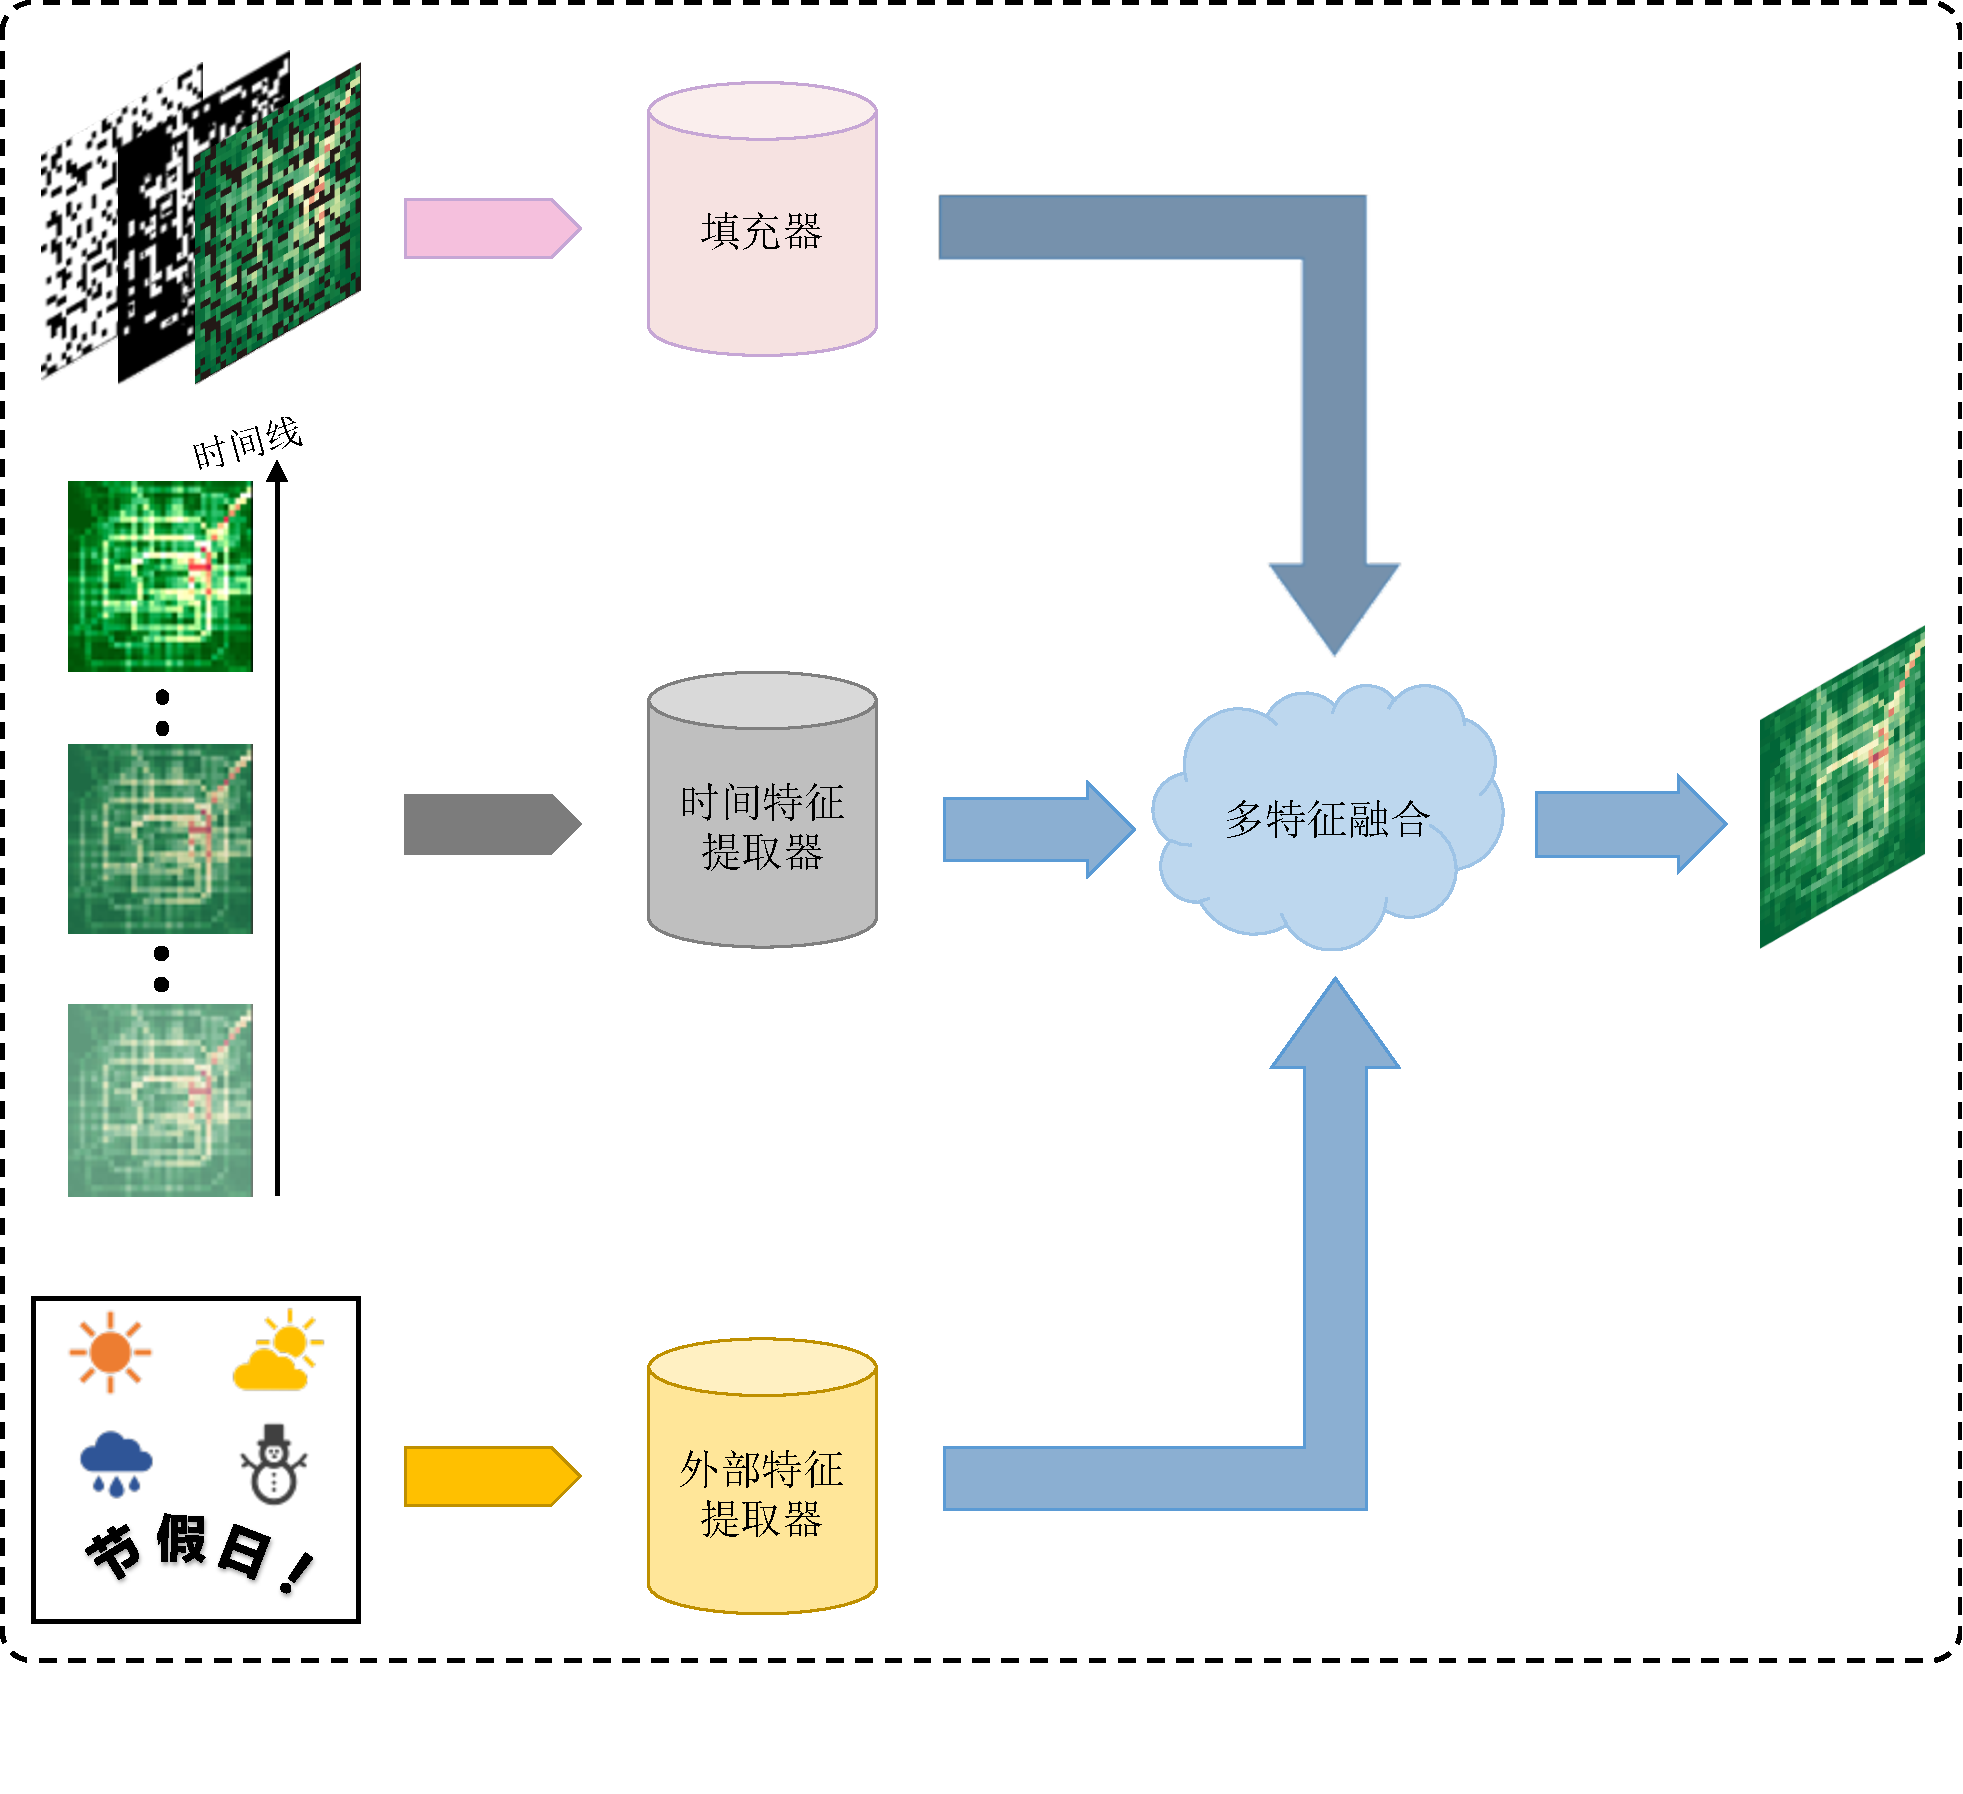
\includegraphics[width = \textwidth]{framework.pdf}
\caption{\textit{ST-LBAVAE}的整体架构图 \label{framework}}
\end{figure}

多层Attention-Biconvgrui时空变分自编码器(\textit{MCST-VAE})由以下三个部分构成。首先是基于可学习的双向注意力图的卷积模块,多层Attention-Biconvgrui模块以及基于标准化流的变分自编码器。以下将按照以上的顺序依次介绍这三部分内容。

\subsection{基于可学习的双向注意力图的卷积模块}
考虑到短期交通数据的缺失值填充场景可以使用历史时刻的完整数据作为参考,因此可以通过对历史数据进行分析来初步提供可能的时间模式,且对时间特征器的设计不需要如填充器一样考虑缺失值的处理问题。

普通卷积模块在处理不含缺失值的数据时取得了良好的效果,但是,交通数据的缺失值带有随机性,即是在雷达图上的缺失地点是不确定的,在时间戳上的缺失时间点也是不确定的,而且不同雷达图上的数值缺失也是不确定的。因而本文需要探求一些新的方法来对这种带有缺失值的交通数据进行有效的建模。针对于在时间戳上的缺失时间点的不确定问题,本文的第一章内容已经设计了$Biconvgrui$模块对带有缺失值的交通数据的时间分布进行有效的建模。为了有效解决普通卷积对雷达图上的数值缺失不敏感问题,本文利用基于可学习的双向注意力图的卷积模块解决此问题。这个方法被左旺孟团队在2019年提出,该方法主要使用了端到端的模型实现了特征再标准化和掩膜矩阵动态更新的效果。具体的表现方式为当特征图在不断地向前传播时,对应的掩膜矩阵$M$也需要不断地更新。即是当特征图在不断地进行采样操作时,对应的观测值也需要进行同步的更新,这种更新的方式主要就是对于掩膜矩阵$M$的持续化更新。参照原论文的方式,具体的更新公式如下所示:

\vspace{-1em}
\begin{subequations}
\begin{align}
\mathbf{F}_{t}^{conv} & = \mathbf{W}^{T}_{pw}f_{bn}(\mathbf{W}^{T}_{dw}\mathbf{F}^{in}_t) \label{dsc_eq} \\
\mathbf{M}^{c}_{t} & = \mathbf{W}^{T}_{m}\mathbf{M}_t  \label{mc_eq}\\
\mathbf{F}_{t}^{out} & = \mathbf{F}_{t}^{conv} \odot f_{A}(\mathbf{M}^{c}_{t})  \label{fr_eq}\\
\mathbf{M}^{'}_{t} & = f_{M}(\mathbf{M}^{c}_{t}) \label{mu_eq},
\end{align}
\end{subequations}

在式子中,$F_in$为模块的输入,$F_conv$为操作的输出,$W_dw$和$W_pw$为卷积操作的参数,在式子中,$W_m$为掩膜卷积操作的参数。在式子中,$\odot$表示哈达玛乘积(Element-wise Product),$f_{A}(\mathbf{M}^{c}_{t})$为可学习的注意力图,具体式子如下所示:
\begin{equation}
    f_{A}(\mathbf{M}^{c}_{t})=
   \begin{cases}
   	\alpha \exp{\big (-\beta(\mathbf{M}^{c}_{t} - \mu)^2 \big)} &\mbox{,若 $\mathbf{M}^{c}_{t} < \mu$}\\
   	1 + (\alpha - 1) \exp{\big ( - \gamma(\mathbf{M}^{c}_{t} - \mu)^2 \big)} &\mbox{,其它}
   \end{cases}
\end{equation}
其中$\alpha$,$\beta$,$\mu$,$\gamma$均为可学习的参数,初始值设置与文献\cite[8861]{xie2019image}同。式子\eqref{mu_eq}表示掩膜的动态更新,具体的更新函数如下所示:
\begin{equation}
    f_{M}(\mathbf{M}^{c}_{t}) = \left [ ReLU(\mathbf{M}^{c}_{t}) \right ]^{\theta}.
\end{equation}

与前向注意力图不同的是,反向注意力图的作用在于聚焦缺失值的修复,即如何运用编码器得到的隐变量信息进行缺失值的预测,所以本文使用与掩膜矩阵$M_t$相反的输入$1-M_t$作为反向注意力图模块的输入。

\begin{figure}[htbp] 
	\centering 
	\subfigure[邻近性]{
		\begin{minipage}[htbp]{0.31\textwidth}
			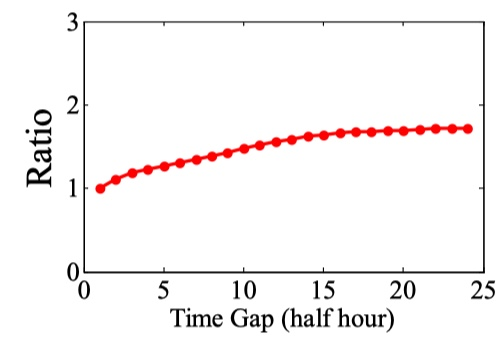
\includegraphics[width=1\textwidth]{closeness} \label{closeness}
		\vspace{-1em}
		\end{minipage}	
	}
	\subfigure[周期性]{
		\begin{minipage}[htbp]{0.31\textwidth}
			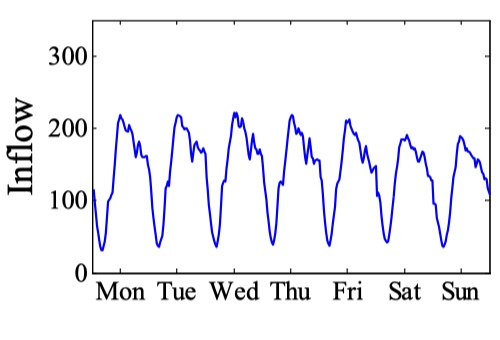
\includegraphics[width=1\textwidth]{period} \label{period}
		\vspace{-1em}
		\end{minipage}
	}
	\subfigure[趋势性]{
		\begin{minipage}[htbp]{0.31\textwidth}
			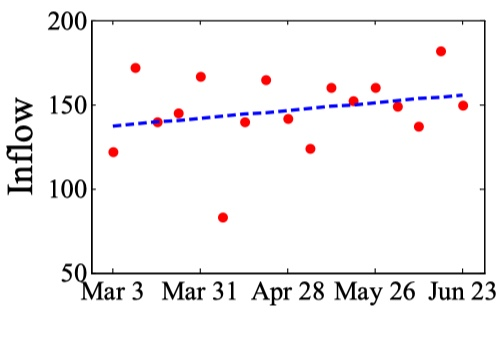
\includegraphics[width=1\textwidth]{trend} \label{trend}
		\vspace{-1em}
		\end{minipage}
	}
	\caption{居民区域入流量(Inflow)的时间依赖性\cite[4]{zhang2017deep}} \label{residual}
\end{figure}

\subsection{多层Attention-Biconvgrui模块}
多层$Biconvgrui$模块是(\textit{MCSTVAE})的一个子模型,它增强了模型提取不完整数据的时间分布特性的能力,并且使得模型能够提取不同时间窗长度的时间相关性。在本章节中,为了进一步增强$Biconvgrui$模块对于交通数据的缺失值的捕捉能力,使用基于可学习的双向注意力图的卷积模块来替换普通的卷积模块。同时,将交通数据按照邻近性,周期性和趋势性三种时间长度划分成三个不同的数据集。同时,将处理邻近性数据集的$Biconvgrui$模型定义为$B_c$, 处理周期性数据集的$Biconvgrui$模型定义为$B_p$,以及处理趋势性数据集的$Biconvgrui$模型定义为$B_t$。给定数据$X_c$,$X_p$以及$X_t$和相应的掩膜矩阵$M_c$,$M_p$和$M_t$作为多层$Biconvgrui$模块的输入,整个多层$Biconvgrui$模块的计算过程,可以用以下公式表示:

\vspace{-1em}
\begin{subequations}
\begin{align}
\mathbf{h}_{c} & = \mathbf{B}_{c}([\mathbf{X}_{c},\mathbf{h}_0]) \label{dsc_eq} \\
\mathbf{F}^{c}_{conv} & = \mathbf{W}^{c}_{pw}\mathbf{M}_t  \label{mc_eq}\\
\mathbf{F}_{t}^{out} & = \mathbf{F}_{t}^{conv} \odot f_{A}(\mathbf{M}^{c}_{t})  \label{fr_eq}\\
\mathbf{M}^{'}_{t} & = f_{M}(\mathbf{M}^{c}_{t}) \label{mu_eq},
\end{align}
\end{subequations}

交通流量可以被多种复杂的外部因素所影响,例如气象、节假日等,如图\ref{extra_features}所示。图\ref{storm}显示了极端天气对于城市人流量的影响,其中红色曲线表示2013年8月11日北京某办公区域的交通入流量,绿色曲线表示2013年8月18日同区域的入流量情况。从图中可以看出当11日下午发生强降雨天气时,该办公区域的人员在下班时间段相较于平时,其入流量出现了骤减的趋势,而18日下午的天气情况为晴朗。图\ref{holiday}展示了2016年北京市某办公区域春节期间(红色)与春节假期结束后一周(绿色)的人流量之间的差异,可以看出在春节期间办公区域的交通入流量比非节假日期间要少很多。因此,将这些额外因素作为极端事件下缺失值的填充是有必要的,它能在特殊情况下为模型提供一些辅助的信息。本文考虑了气象情况、节假日和周末这些外部因素,其中气象情况又包含了天气、气温和风速信息。

\begin{figure}[htbp] 
	\centering 
	\subfigure[强降雨和正常天气下的城市人流量]{
		\begin{minipage}[htbp]{0.48\textwidth}
			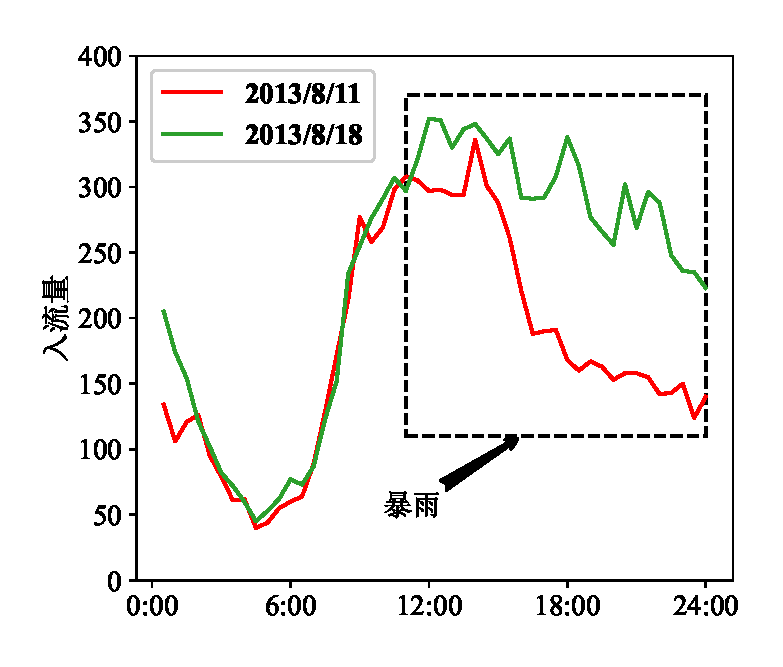
\includegraphics[width=1\textwidth]{storm2} \label{storm}
%		\vspace{-1em}
		\end{minipage}	
	}
	\subfigure[(非)节假日的城市人流量]{
		\begin{minipage}[htbp]{0.48\textwidth}
			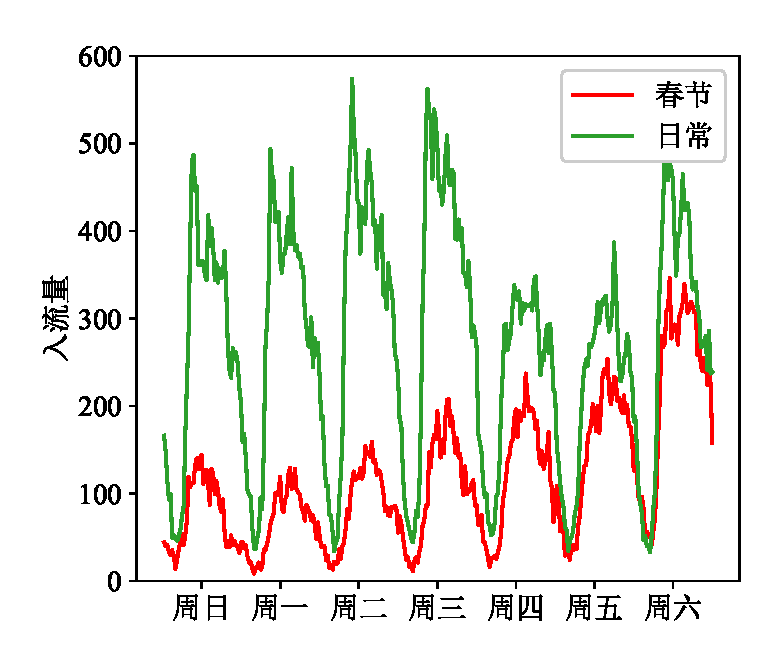
\includegraphics[width=1\textwidth]{holiday2} \label{holiday}
%		\vspace{-1em}
		\end{minipage}
	}
	\caption{外部因素对北京市某办公区域入流量的影响} \label{extra_features}
\end{figure}

考虑到额外数据的离散性,本文将离散数据用独热编码(One-Hot Encoding)的方式进行处理,这样单个离散的值便可以用向量的形式来表示,向量的长度即为离散值的状态数,进而实现了将离散属性数据映射到欧式空间的目的,便于计算离散属性数据之间的相似性。以工作日/周末特征为例,本文用一个八位只有0和1的二值向量来表示它。前七位表示周一至周日,最后一位表示是否为非工作日,若为非工作日,则标记为1,比如星期一用独热编码后的向量为$(1, 0, 0, 0,0,0,0,1)$。

本文设计了外部特征提取器来完成外部信息的表示,具体结构如图\ref{extra_extractor}所示。假设处理后的额外数据为$\mathbf{E}_t$,首先使用一个嵌入层加$ReLU$激活函数将其从高维空间非线性地映射到低维空间,用于特征的压缩,同时也可以减少网络训练的参数量,接着最后使用另一个全连接层和$Reshape$操作来保证最后输出的形状能与待填充栅格图$\mathbf{X}_t$相匹配,便于之后的多特征融合,记外部特征提取器的输出为$\mathbf{X}_t^{ext}$。

\begin{figure}[htbp]
\centering
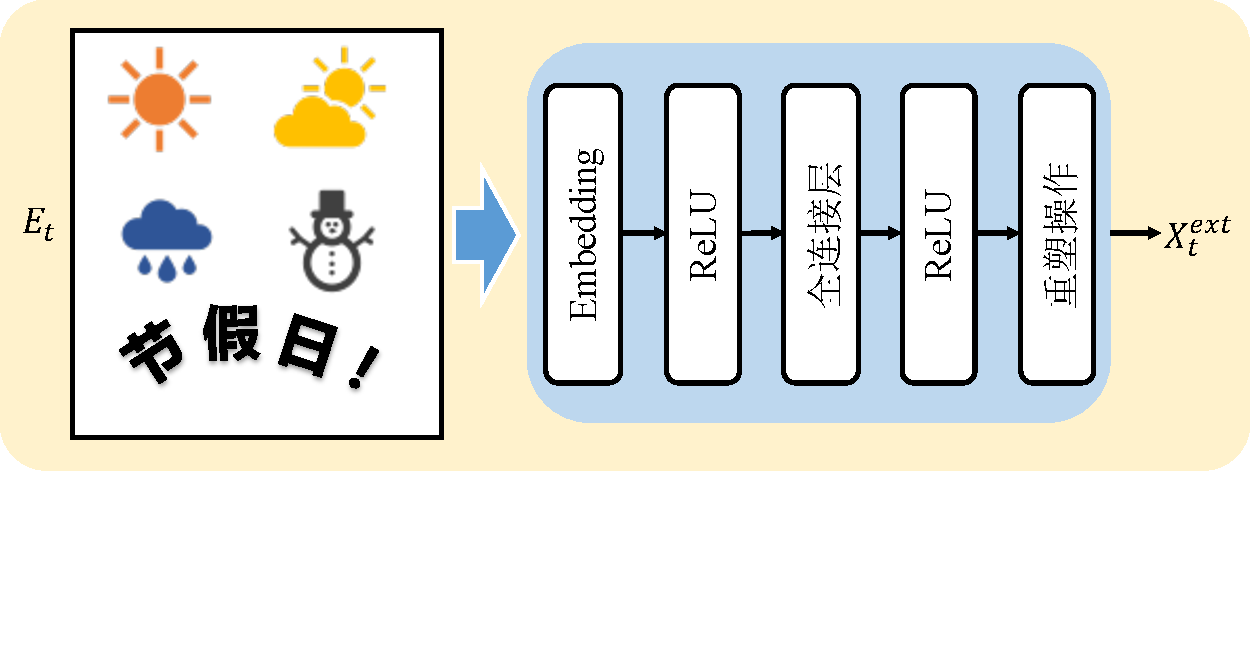
\includegraphics[width = 0.9\textwidth]{extra_extractor.pdf}
\vspace{-4em}
\caption{外部特征提取器的结构图 \label{extra_extractor}}
\end{figure}

\subsection{填充器}
本文设计了带有轻量级的双向可学习注意力图的变分自编码器来进行缺失值的填充,如图\ref{filler}所示。它包含编码器、随机隐变量表达层和解码器,编码器由多个下采样层组成,解码器由多个上采样层组成。

\begin{figure}[htbp]
\centering
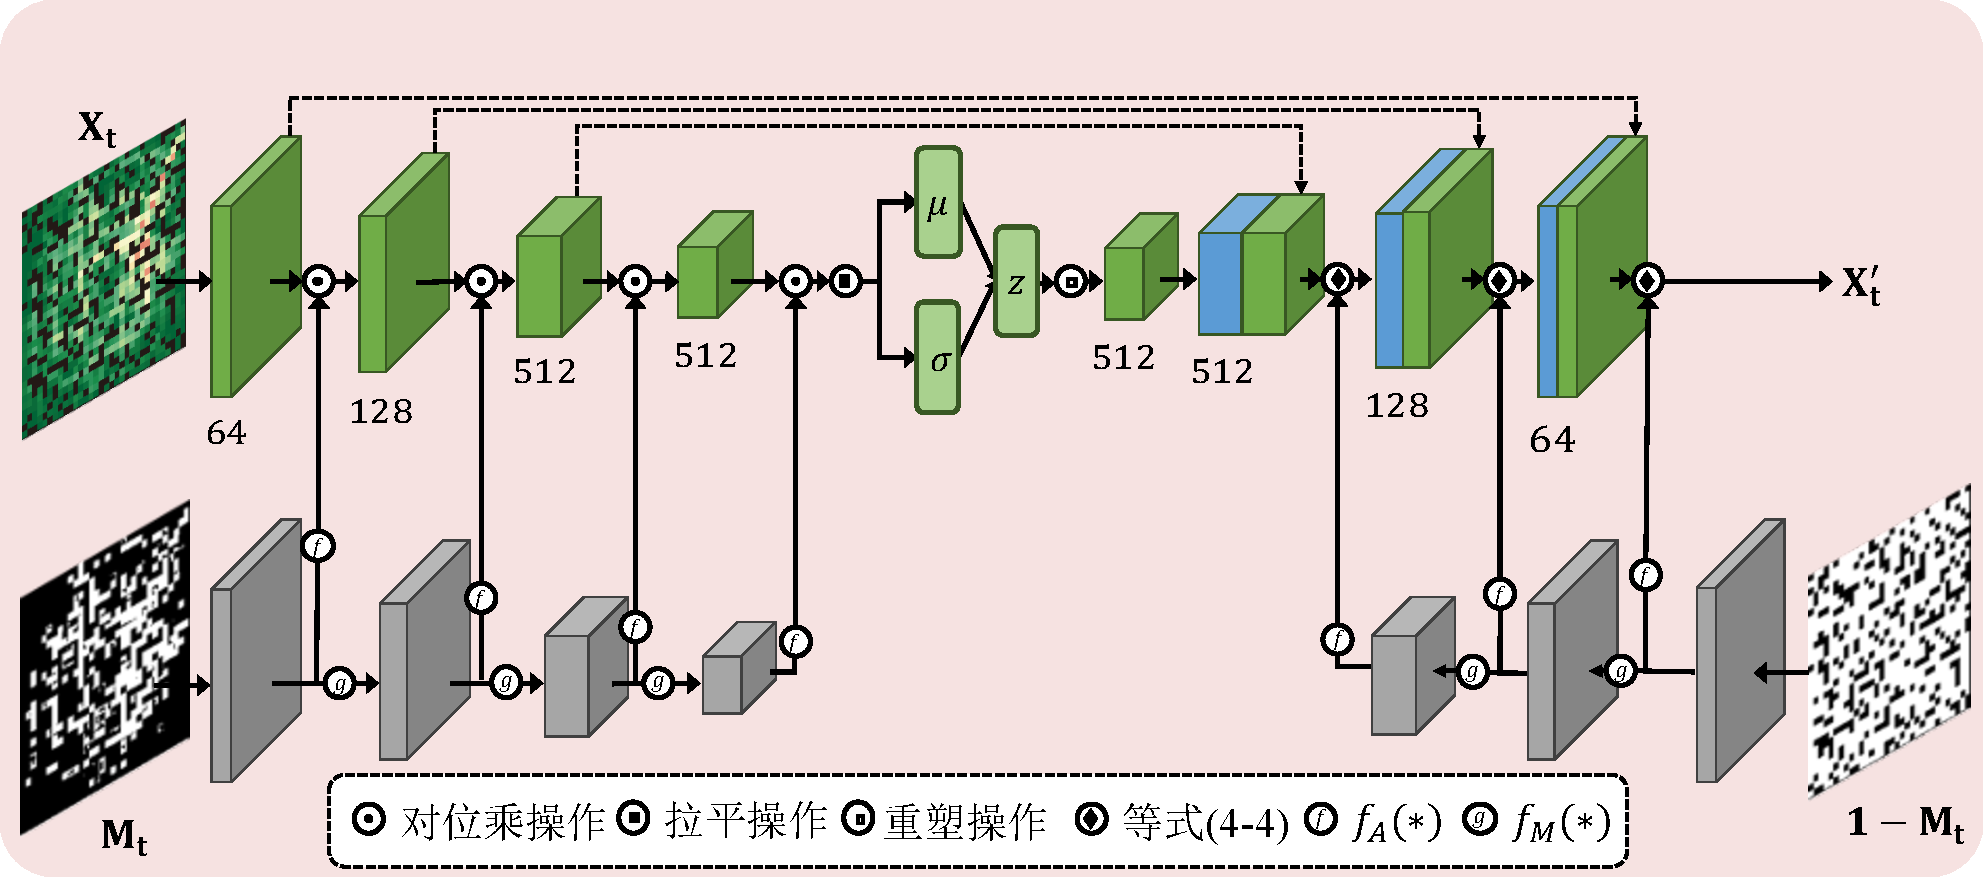
\includegraphics[width = \textwidth]{filler.pdf}
\vspace{-1em}
\caption{轻量级双向可学习注意力变分自编码器 \label{filler}}
\end{figure}

填充器以待填充的交通栅格图$\mathbf{X}_t$作为输入,同时还使用了待填充数据的掩膜矩阵$\mathbf{M}_t$,在$\mathbf{M}_t$中,元素值1表示栅格图$\mathbf{X}_t$中对应位置的值可以被观测到,0表示对应位置的值是缺失值。$\mathbf{X}_t$和$\mathbf{M}_t$每次经过下采样层,其特征图的尺寸都会缩减为原来的一半,但是通道数会翻倍;相反,经过上采样层的时候,特征图的尺寸会扩大为原来的两倍,但是通道数会减少为原来的一半。由多个下采样层组成的编码器输出随机隐变量的均值$\mu$和标准差$\sigma$,再通过重参数化技巧得到随机隐变量$z$,主要过程与式子\eqref{vae_equation_d}一致。接着随机隐变量$z$通过解码器上采样后得到初步还原的栅格图$\mathbf{X}_{t}^{'}$,在解码阶段还用到了与$\mathbf{M}_t$相反的输入$1-\mathbf{M}_t$11。

\begin{figure}[htbp] 
	\centering 
	\subfigure[前向可学习注意力图]{
		\begin{minipage}[htbp]{0.48\textwidth}
			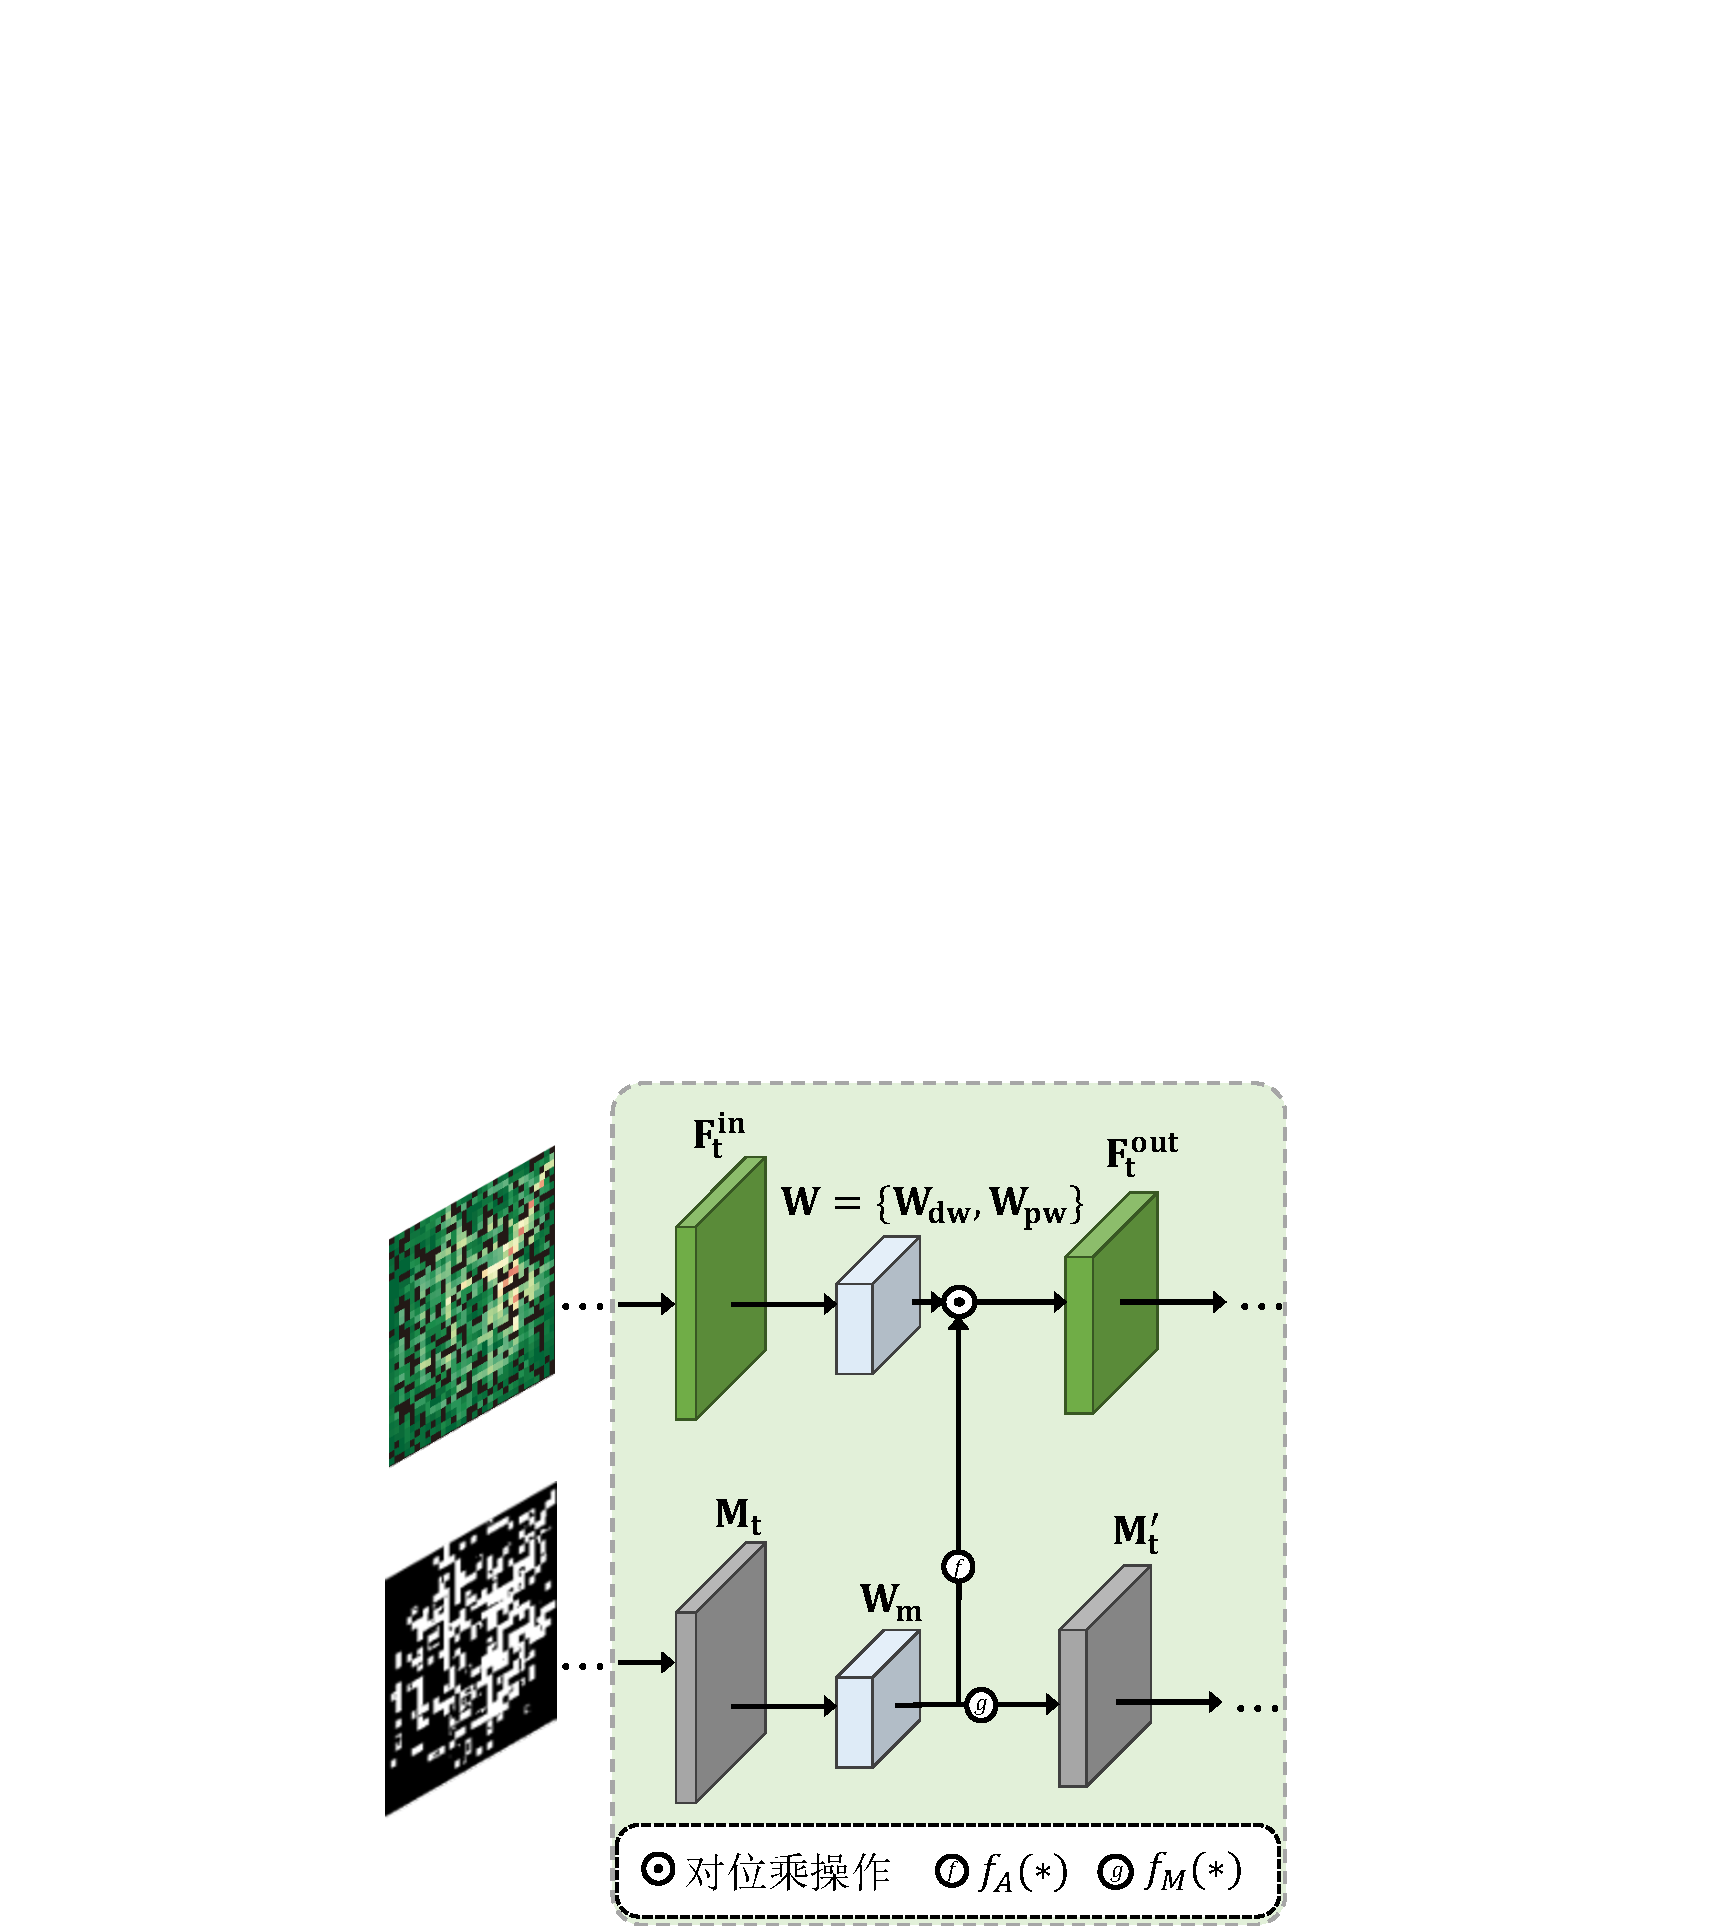
\includegraphics[width=1.03\textwidth]{forward_llbam.pdf} \label{forward_llbam}
%		\vspace{-1em}
		\end{minipage}	
	}
	\subfigure[反向可学习注意力图]{
		\begin{minipage}[htbp]{0.48\textwidth}
			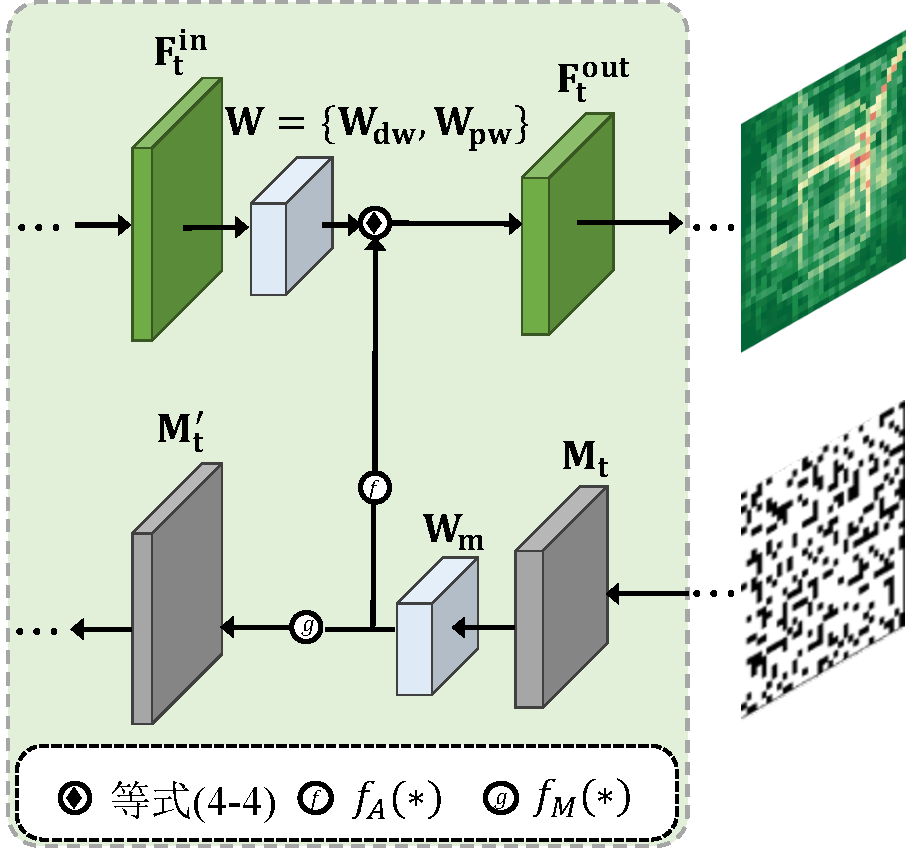
\includegraphics[width=1.0\textwidth]{reverse_llbam.pdf} \label{reverse_llbam}
%		\vspace{-1em}
		\end{minipage}
	}
	\caption{轻量级双向可学习注意力图模块} \label{llbam}
\end{figure}

额外地,考虑到城市交通数据的缺失情况具有随机性,即缺失的地点是不确定的,缺失的时间戳是不确定的,同时缺失的比例也是预先未知的,而当前的基于深度学习的交通数据缺失值填充算法\cite{yu20193d,boquet2019missing}很难处理这种情况。为了模拟实际场景中不规则的交通流的缺失值分布情况,本文利用可学习的双向注意力图模块\cite{xie2019image}解决了此问题,该模块于2019年被左旺孟团队提出,主要以一种端到端的方式来达到特征再标准化和掩膜矩阵动态更新的效果,具体表现为在特征图向前传播的同时,掩膜矩阵也会随之进行动态更新,即随着特征图不断地下采样,对应的观测值的信息也需要不断被更新,而这个更新的指示器就是可更新的掩膜矩阵$\mathbf{M}_t$,本文将其做了模块轻量化的改进,故称为轻量级可学习注意力图,如图\ref{llbam}所示。它主要可以分为四个操作:(1)深度可分离卷积(Depth-wise Separable Convolution);(2)掩膜卷积(Mask Convolution);(3)特征再标准化(Feature Re-Normalization);(4)掩膜更新(Mask Updating)。可用如下式子表示:
\vspace{-1em}
\begin{subequations}
\begin{align}
\mathbf{F}_{t}^{conv} & = \mathbf{W}^{T}_{pw}f_{bn}(\mathbf{W}^{T}_{dw}\mathbf{F}^{in}_t) \label{dsc_eq} \\
\mathbf{M}^{c}_{t} & = \mathbf{W}^{T}_{m}\mathbf{M}_t  \label{mc_eq}\\
\mathbf{F}_{t}^{out} & = \mathbf{F}_{t}^{conv} \odot f_{A}(\mathbf{M}^{c}_{t})  \label{fr_eq}\\
\mathbf{M}^{'}_{t} & = f_{M}(\mathbf{M}^{c}_{t}) \label{mu_eq},
\end{align}
\end{subequations}
在式子\eqref{dsc_eq}中,$\mathbf{F}^{in}_t$为模块的输入,$\mathbf{F}^{conv}_t$为操作(1)的输出,$\mathbf{W}_{dw}$和$\mathbf{W}_{pw}$为深度可分离卷积\cite{chollet2017xception}的两次卷积操作(Depth-wise $\&$ Point-wise Convolution)的参数,两次卷积中穿插了一个批标准化操作$f_{bn}$。相较于普通卷积,深度可分离卷积极大地减少了网络的训练参数,以本文的数据集TaxiBJ中的输入样本为例,输入形状为$[1,32,32]$,则输出形状为$[64,16,16]$的特征图需要使用64个$3 \times 3$的卷积核(参数量为576),而使用深度可分离卷积需要使用1个$3 \times 3$的卷积核和64个$1 \times 1$的卷积核(参数量为73),比较之下后者的训练参数减少了$87\%$。在式子\eqref{mc_eq}中,$\mathbf{W}_m$为掩膜卷积操作的参数。在式子\eqref{fr_eq}中,$\odot$表示哈达玛乘积(Element-wise Product),$f_{A}(\mathbf{M}^{c}_{t})$为可学习的注意力图,具体式子如下所示:
\begin{equation}
    f_{A}(\mathbf{M}^{c}_{t})=
   \begin{cases}
   	\alpha \exp{\big (-\beta(\mathbf{M}^{c}_{t} - \mu)^2 \big)} &\mbox{,若 $\mathbf{M}^{c}_{t} < \mu$}\\
   	1 + (\alpha - 1) \exp{\big ( - \gamma(\mathbf{M}^{c}_{t} - \mu)^2 \big)} &\mbox{,其它}
   \end{cases}
\end{equation}
其中$\alpha$,$\beta$,$\mu$,$\gamma$均为可学习的参数,初始值设置与文献\cite[8861]{xie2019image}同。式子\eqref{mu_eq}表示掩膜的动态更新,具体的更新函数如下所示:
\begin{equation}
    f_{M}(\mathbf{M}^{c}_{t}) = \left [ ReLU(\mathbf{M}^{c}_{t}) \right ]^{\theta}.
\end{equation}

轻量级的可学习注意力图被应用于填充器的编码阶段,用于表示随着特征图不断地下采样,对应的观测值的信息也需要不断被更新,又称为前向注意力图。不难理解,该注意力图主要用于有针对性地提取有效位置的数据的特征。

同时,本文使用U-Net\cite{ronneberger2015u}结构将编码器中第$l$层的特征图与解码器中第$L-l$层的特征图拼接起来作为解码器中第$L-l+1$层的输入。其本质是通过跳跃连接融合不同层次的语义特征,使得特征的表达更加的准确。假设用$\mathbf{F}^{conv}_e$和$\mathbf{F}^{conv}_d$分别表示经过深度可分离卷积后的编码器和解码器的特征图,$\mathbf{M}^{c}_e$和$\mathbf{M}^{c}_d$分别表示编码器和解码器的卷积后的掩膜,基于U-Net结构,则解码器中的特征再标准化操作可以改写为如下式子:
\begin{equation}
	\mathbf{F}_{d}^{out} = \mathbf{F}^{conv}_e \odot f_{M}(\mathbf{M}^{c}_{e}) + \mathbf{F}^{conv}_d \odot f_{M}(\mathbf{M}^{c}_{d}),
\end{equation}
与前向注意力图不同的是,反向注意力图的作用在于聚焦缺失值的修复,即如何运用编码器得到的隐变量信息进行缺失值的预测,故本文使用与掩膜矩阵$M_t$相反的输入$1-M_t$作为反向注意力图模块的输入。

此外,由于输入的只是单时间槽的栅格数据,因此,该填充器使用2D卷积专注于交通流量中空间相关性的建模。



\subsection{多特征融合机制}
关于多特征融合,一般有两种方式,一种是相加操作,另一种是拼接操作。本文首先将填充器输出的特征图$\mathbf{X}_t^{'}$与时间提取器输出的特征图$\widetilde{\mathbf{X}}_t$进行相加,最后将其与外部特征的输出$\mathbf{X}_t^{ext}$进行拼接操作,如下式所示:
\begin{subequations} \label{fusion_eq}
\begin{align}
	H_t(:,c,:,:) & = \mathbf{X}_t^{'}(:,c,:,:) + \widetilde{\mathbf{X}}_t(:,c,:,:), c=0,...,C-1 \\
	H_t(:,C,:,:) & = \mathbf{X}_t^{ext},
\end{align}
\end{subequations}
这样做的原因是时空特征是复杂的,通过相加操作能有助于时空模式的建立,而外部特征会间接地影响时空特征的极端表示,故将其拼接最后通过卷积核大小为$1\times 1$,步长为1的2D卷积操作进行通道特征的融合。



\section{目标函数和模型训练} \label{sec4_5}
为了更好地恢复交通数据的上下文细节和语义特征,本文引入了变分自编码器损失、感知损失和风格损失来训练\textit{ST-LBAVAE}。

(1)\textbf{变分自编码器损失函数}:该损失函数主要由三部分组成,分别为观测值重建误差、缺失值误差和随机隐变量分布的$KL$散度。记真实完整样本为$X$,重建样本为$\hat{X}$,掩膜矩阵为$M$,则观测值重建误差如下式所示:
		\begin{equation}
			Loss_1 = \frac{1}{n}\sum_{i=1}^{n}((X \otimes M)_i - (\hat{X} \otimes M)_i)^2
		\end{equation}
		其中$n$为缺失值的数量,$\otimes$表示元素对位相乘。
		
		缺失值重建误差如下式所示:
		\begin{equation}
			Loss_2 = \frac{1}{n}\sum_{i=1}^{n}((X \otimes (1-M))_i - (\hat{X} \otimes (1-M))_i)^2
		\end{equation}
		
		$KL$散度损失如下式所示:
		\begin{equation}
			Loss_3 = -\frac{1}{2} \sum_{j=1}^{D}\bigg (1+ \log{\sigma_j^2} - \mu_j^2 - \sigma_j^2\bigg )
		\end{equation}
		其中,$D$表示随机隐变量的维数。
		
(2)\textbf{感知损失函数}:变分自编码器损失中的前两项只是简单地计算了真实值与预测值之间的误差,但是忽略了交通数据中更加高层的语义信息。本文通过将真实样本和重建样本分别输入到在Imagenet\cite{russakovsky2015imagenet}上进行了预训练的VGG-16模型\cite{simonyan2014very}来衡量高层特征之间的误差,即感知损失,如下式所示:
		\begin{equation}
			Loss_4 = \frac{1}{N} \sum_{k=1}^{N}\frac{1}{n}\sum_{i=1}^{n}(\mathcal{P}_{k}(X) - \mathcal{P}_{k}(\hat{X}))^2,
		\end{equation}
		其中,$\mathcal{P}_{k}(\cdot)$表示VGG-16模型中第$k$个池化层的特征图。本文使用了其中的三层池化层,即$N=3$。

(3)\textbf{风格损失函数}:为了更好地还原交通数据的上下文信息,本文引入了风格损失函数。它用于衡量由VGG-16模型输出的特征图之间$Gram$矩阵的相似性,假设特征图$\mathcal{P}_{k}(\cdot)$的尺寸为$C_k \times H_k \times W_k$,则风格损失函数如下式子所示:
		\begin{equation}
			Loss_5 = \frac{1}{N} \sum_{k=1}^{N} \frac{1}{n \times C_k^2}\sum_{i=1}^{n}(\mathcal{P}_{k}(X)(\mathcal{P}_{k}(X)^T - \mathcal{P}_{k}(\hat{X})\mathcal{P}_{k}(\hat{X})^T)^2.
		\end{equation}

综合上述五个损失函数,\textit{ST-LBAVAE}的目标函数用如下式子表示:
\begin{equation}
	\mathcal{L} = \lambda_1 Loss_1 + \lambda_2 Loss_2 + \lambda_3 Loss_3 + \lambda_4 Loss_4 + \lambda_5 Loss_5 \label{lbavae_loss}
\end{equation}
其中$\lambda_1=1.0, \lambda_2=6.0, \lambda_3=1.0, \lambda_4=0.05, \lambda_5=120$。
 
本文可以通过梯度下降法优化式子\eqref{lbavae_loss}的方式来线下训练\textit{ST-LBAVAE}。下面给出训练\textit{ST-LBAVAE}模型的伪代码,如下所示。
\begin{algorithm}[htbp]
	\floatname{algorithm}{算法} 
	\renewcommand{\algorithmicrequire}{\textbf{输入:}}
	\renewcommand{\algorithmicensure}{\textbf{输出:}}
	\caption{\quad \textit{ST-LBAVAE} 训练算法}
	\label{alg1}
	\begin{algorithmic}[1]
		\REQUIRE 历史完整数据$\{X_0, X_1, \dots,X_{n-1}  \}$;对应掩膜矩阵$\{M_0, M_1, \dots,M_{n-1}  \}$;外部因素$\{E_0, E_1, \dots,E_{n-1}  \}$;邻近、周期、趋势属性数据片段的长度$l_c, l_p, l_q$;周期定义长度$p$;趋势定义长度$q$。
		
		\ENSURE 学习完参数的\textit{ST-LBAVAE}模型
		
		\textbf{步骤 1}: 构建训练样本集 
		
		\STATE 使用最大最小归一化将数据范围缩到区间$[-1, 1]$
		
		\STATE $\mathcal{D} \longleftarrow \emptyset$
		
		\FOR {$t = 1$ to $n-1$}
			\STATE $\mathcal{S}_c$ = [$X_{t-l_c}, X_{t-({l_c-1})}, \dots, X_{t-1}$]
			\STATE $\mathcal{S}_p$ = [$X_{t-l_p \cdot p}, X_{t-({l_p-1}) \cdot p}, \dots, X_{t-p}$]
			\STATE $\mathcal{S}_q$ = [$X_{t-l_q \cdot q}, X_{t-({l_q-1}) \cdot q}, \dots, X_{t-q}$]
			\STATE 将缺失值用零进行预填充,获得预处理后的样本$\widetilde{X_{t}}$
			\STATE 将元组$(X_t, M_t, \mathcal{S}_c, \mathcal{S}_p, \mathcal{S}_q, \widetilde{X_{t}})$作为一个样本放入数据集$\mathcal{D}$
		\ENDFOR
		
		\textbf{步骤 2}: 训练\textit{ST-LBAVAE}模型
		 
		\STATE 初始化\textit{ST-LBAVAE}中所有可学习的参数
		\REPEAT
		\STATE 随机从$\mathcal{D}$中选择一批次的样本$X_b$
		\STATE $\varphi, \theta \longleftarrow$ 使用Adam优化器更新参数 
		\UNTIL 目标函数$\mathcal{L}$收敛
	\end{algorithmic}  
\end{algorithm}


\section{实验与分析} \label{sec4_7}
本小节首先介绍了实验所需要用的数据集,然后列出了实验环境和模型参数的设置,接着进行了对比实验和模型复杂度的分析,最后给出了消融实验的结果。
\subsection{数据集}
为了定量地评价所提出的模型的填充效果,本文使用了TaxiBJ\cite{zhang2017deep}和BikeNYC\cite{zhang2017deep}数据集,数据集描述如表\ref{tb_dataset}所示。

以上轨迹数据均可通过定义(\ref{def_flow})转换为交通出入流量数据。本文按照五个缺失值比例10\%,30\%,50\%,70\%,90\%随机手动生成相应的数据集。接着使用归一化将数据集数值范围缩放到区间[-1,1]内。对于每个数据集,本文将数据集前90\%的样本作为训练集,剩余的样本作为测试集,又取训练集中的90\%作为验证集。为了防止模型训练产生过拟合现象,我们保存在验证集上损失函数最小的模型参数用于测试。

\subsection{实验设置} \label{setup}
(1)\textbf{实验环境}:本章实验均在GPU服务器上完成,表\ref{env1}给出了实验所采用的软硬件环境的具体细节。

\begin{table}[htbp] \footnotesize
\caption{ 实验软硬件环境} \label{env2}
\vspace{0.5em}\centering\wuhao
\begin{tabular}{cc}
\toprule[1.5pt]
环境 & 参数\\
\midrule[1pt]
操作系统 & Ubuntu 20.04.2.0 LTS \\
内存 & 128GB \\
磁盘 & 1TB SSD \\
处理器 & 英特尔至强Gold 5218R@2.10GHz \\
图形卡 & GeForce RTX 3080 \\
CUDA版本 & 11.1 \\
开发语言 & Python 3.8 \\
深度学习框架 & Pytorch 1.8.1 \\
\bottomrule[1.5pt]
\end{tabular}
\end{table}

(2)\textbf{模型超参设置:}每一个3D卷积模块的卷积核均设置为$3\times 3 \times3$,随机隐变量$z$的长度固定为128,周期定义长度$p$为一天,趋势定义长度$q$为一星期,$l_c$在$\{1, 2, 3, 4\}$中取值,$l_p$在$\{2, 3, 4\}$中取值,$l_q$在$\{2, 3, 4\}$中取值。本实验采用Adam优化器来进行梯度优化,且初始学习率为$10^{-3}$,一阶矩估计和二阶矩估计的指数衰减率分别为$0.5$和$0.9$。最后,模型在TaxiBJ和BikeNYC上的训练周期数均为200。

(3)\textbf{评价指标:}本文采用均方根误差(RMSE)和平均绝对误差(MAE)作为模型评价的指标,具体公式如下所示:
\begin{equation}
\mathrm{RMSE}=\sqrt{\mathbb{E}\big \{ \left\|(1-m) \otimes \left(x-\hat{x}\right)\right\|_{F} \big \}}
\end{equation}
\begin{equation}
\mathrm{MAE}=\mathbb{E}\big \{ \left\|(1-m) \otimes \left(x-\hat{x}\right)\right\|_{1} \big \}
\end{equation}
%\begin{equation}
%\mathrm{NMSE}=\mathbb{E}\bigg \{\frac{\left\|(1-m) \otimes \left(x-\hat{x}\right)\right\|_{F}}{\left\|(1-m) \otimes x\right\|_{F}} \bigg \}
%\end{equation}

\subsection{对比实验结果与分析}
为了验证\textit{ST-LBAVAE}模型在短期交通数据缺失值填充中的优越性,本文与九个基线模型(Baselines)进行了对比,分别为HA、ConvLSTM\cite{shi2015convolutional}、ST-ResNet\cite{zhang2017deep}、TF-3DNet\cite{yu20193d}、PPCA\cite{qu2009ppca}、Time-KNN、HaLRTC\cite{ran2016tensor}、MLP-VAE\cite{boquet2019missing}、ST-LBAGAN\cite{yang2021st}。本文使用了基线模型所提出论文中的超参来配置对比模型。

表\ref{rmse_taxibj}和表\ref{mae_taxibj}分别展示了各个模型在TaxiBJ数据集上的表现。表\ref{rmse_bikenyc}和表\ref{mae_bikenyc}分别显示了各个模型在BikeNYC数据集上的表现。

%\vspace{-1.5bp}
%\ltfontsize{\wuhao[1.667]}
%\wuhao[1.667]\begin{longtable}{lccccc}
%\caption{\wuhao 中国省级行政单位一览}\\
%\toprule[1.5pt] 名称 & 简称 & 省会或首府  \\ \midrule[1pt]
%\endfirsthead
%\multicolumn{3}{r}{表~\thetable(续表)}\vspace{0.5em}\\
%\toprule[1.5pt] 名称 & 简称 & 省会或首府  \\ \midrule[1pt]
%\endhead
%\bottomrule[1.5pt]
%\endfoot
%北京市 & 京 & 北京\\
%
%\end{longtable}\normalsize
%\vspace{-1em}
\begin{table}[htbp] 
\caption{TaxiBJ数据集的RMSE指标对比} \label{rmse_taxibj}
\vspace{0.5em}\centering\wuhao
\begin{tabular*}{\hsize}{@{}@{\extracolsep{\fill}}lccccc@{}}
\toprule[1.5pt]
缺失率 & 10\% & 30\% & 50\% & 70\% & 90\%\\
\midrule[1pt]
HA              & 39.86 & 39.97 & 40.06 & 40.00  & 39.98  \\
ConvLSTM  & 18.98 & 19.06 & 19.06 & 19.08  & 19.10  \\
ST-ResNet & 16.86 & 16.95 & 16.96 & 16.96  & \textbf{16.96}  \\
TF-3DNet  & 17.43 & 17.48 & 17.48 & 17.47  & 17.49  \\
PPCA            & 23.94 & 49.52 & 77.32 & 106.45 & 135.25 \\
Time-KNN        & 21.33 & 24.37 & 29.32 & 38.90  & 56.68  \\
HaLRTC    & 32.25 & 37.08 & 43.97 & 62.78  & 140.01 \\
MLP-VAE   & 24.34 & 31.77 & 43.42 & 57.68  & 74.05  \\
ST-LBAGAN    & 12.86 & 13.23 & 14.29 & 15.49  & 17.95  \\
ST-LBAVAE(ours) & \textbf{12.37} & \textbf{12.86} & \textbf{13.70} & \textbf{14.94}  & 17.25 \\
\bottomrule[1.5pt]
\end{tabular*}
\end{table}

\begin{table}[htbp] 
\caption{TaxiBJ数据集的MAE指标对比} \label{mae_taxibj}
\vspace{0.5em}\centering\wuhao
\begin{tabular*}{\hsize}{@{}@{\extracolsep{\fill}}lccccc@{}}
\toprule[1.5pt]
缺失率 & 10\% & 30\% & 50\% & 70\% & 90\%\\
\midrule[1pt]
HA        & 18.80  & 18.80   & 18.86   & 18.84   & 18.83          \\
ConvLSTM  & 12.50  & 12.49   & 12.46   & 12.48   & 12.49          \\
ST-ResNet & 11.16  & 11.19   & 11.19   & 11.19   & \textbf{11.19} \\
TF-3DNet  & 11.97  & 11.97   & 11.96   & 11.96   & 11.97          \\
PPCA      & 13.68  & 29.55   & 47.45   & 66.05   & 84.41          \\
Time-KNN  & 12.18  & 13.81   & 16.45   & 21.61   & 31.66          \\
HaLRTC    & 17.43  & 19.97   & 23.67   & 34.43   & 86.45          \\
MLP-VAE   & 15.80  & 20.64   & 28.65   & 38.66   & 50.04          \\
ST-LBAGAN    & 8.70   & 8.88    & 9.52   & 10.18   & 11.64          \\
ST-LBAVAE(ours)& \textbf{8.54} & \textbf{8.79} & \textbf{9.35} & \textbf{10.05} & 11.54  \\
\bottomrule[1.5pt]
\end{tabular*}
\end{table}

%\begin{table}[htbp] 
%\caption{TaxiBJ数据集的NMSE指标对比} \label{nmse_taxibj}
%\vspace{0.5em}\centering\wuhao
%\begin{tabular*}{\hsize}{@{}@{\extracolsep{\fill}}lccccc@{}}
%\toprule[1.5pt]
%缺失率 & 10\% & 30\% & 50\% & 70\% & 90\%\\
%\midrule[1pt]
%HA        & 0.5795 & 0.5706 & 0.5770 & 0.5726 & 0.5736 \\
%ConvLSTM  & 0.1297 & 0.1311 & 0.1342 & 0.1332 & 0.1343 \\
%ST-ResNet & 0.1132 & 0.1153 & 0.1171 & 0.1158 & 0.1168 \\
%TF-3DNet  & 0.1224 & 0.1231 & 0.1255 & 0.1245 & 0.1255 \\
%PPCA      & 0.0351 & 0.1153 & 0.2692 & 0.5011 & 0.8089 \\
%Time-KNN  & 0.1813 & 0.2369 & 0.3741 & 0.7104 & 1.4513 \\
%HaLRTC    & 0.1499 & 0.1751 & 0.1905 & 0.2207 & 0.8511 \\
%MLP-VAE   & 0.0817 & 0.3454 & 0.9764 & 2.0013 & 3.2922 \\
%ST-LBAGAN    & 0.0185 & 0.0200 & 0.0257 & 0.0328 & 0.1959 \\
%ST-LBAVAE(ours) & \textbf{0.0139} & \textbf{0.0149} & \textbf{0.0163} & \textbf{0.0225} & \textbf{0.0561}  \\
%\bottomrule[1.5pt]
%\end{tabular*}
%\end{table}


\begin{table}[htbp] 
\caption{BikeNYC数据集的RMSE指标对比} \label{rmse_bikenyc}
\vspace{0.5em}\centering\wuhao
\begin{tabular*}{\hsize}{@{}@{\extracolsep{\fill}}lccccc@{}}
\toprule[1.5pt]
缺失率 & 10\% & 30\% & 50\% & 70\% & 90\%\\
\midrule[1pt]
HA        & 6.84 & 6.36  & 6.51  & 6.31  & 6.34 \\
ConvLSTM  & 7.33 & 7.62  & 7.66  & 7.45  & 7.54 \\
ST-ResNet & 4.78 & 4.79  & 4.83  & 4.76  & 4.77 \\
TF-3DNet  & 4.28 & 4.31  & 4.34  & 4.27  & \textbf{4.28} \\
PPCA      & 6.92 & 9.43  & 13.23 & 16.47 & 20.09 \\
Time-KNN  & 6.71 & 8.39  & 10.00 & 12.13 & 16.56 \\
HaLRTC    & 5.54 & 5.54  & 9.92  & 14.04 & 19.77 \\
MLP-VAE   & 8.79 & 10.06 & 11.83 & 13.36 & 14.89 \\
ST-LBAGAN & 4.45 & 4.76  & 4.97  & 5.11  & 5.87 \\
ST-LBAVAE(ours) & \textbf{3.29} & \textbf{3.48} & \textbf{3.83} & \textbf{4.09} & \textbf{4.28}  \\
\bottomrule[1.5pt]
\end{tabular*}
\end{table}

\begin{table}[htbp] 
\caption{BikeNYC数据集的MAE指标对比} \label{mae_bikenyc}
\vspace{0.5em}\centering\wuhao
\begin{tabular*}{\hsize}{@{}@{\extracolsep{\fill}}lccccc@{}}
\toprule[1.5pt]
缺失率 & 10\% & 30\% & 50\% & 70\% & 90\%\\
\midrule[1pt]
HA        & 2.84 & 2.77  & 2.80  & 2.72  & 2.75 \\
ConvLSTM  & 4.45 & 4.41  & 4.42  & 4.30  & 4.35 \\
ST-ResNet & 2.74 & 2.64  & \textbf{2.66}  & \textbf{2.62}  & \textbf{2.62} \\
TF-3DNet  & 2.88 & 2.82  & 2.83  & 2.78  & 2.79 \\
PPCA      & 3.01 & 4.13  & 5.84  & 7.43  & 9.14 \\
Time-KNN  & 3.00 & 3.59  & 4.23  & 5.28  & 7.78 \\
HaLRTC    & 2.47 & 2.79  & 3.84  & 5.57  & 8.59 \\
MLP-VAE   & 5.65 & 6.25  & 7.32  & 8.25  & 9.18 \\
ST-LBAGAN & 2.78 & 2.79  & 2.87  & 2.88  & 3.39 \\
ST-LBAVAE(ours) & \textbf{2.45} & \textbf{2.58} & 2.72 & 2.90 & 3.02  \\
\bottomrule[1.5pt]
\end{tabular*}
\end{table}

%\begin{table}[htbp] 
%\caption{BikeNYC数据集的NMSE指标对比} \label{nmse_bikenyc}
%\vspace{0.5em}\centering\wuhao
%\begin{tabular*}{\hsize}{@{}@{\extracolsep{\fill}}lccccc@{}}
%\toprule[1.5pt]
%缺失率 & 10\% & 30\% & 50\% & 70\% & 90\%\\
%\midrule[1pt]
%HA        & 6.84 & 6.36  & 6.51  & 6.31  & 6.34 \\
%ConvLSTM  & 7.33 & 7.62  & 7.66  & 7.45  & 7.54 \\
%ST-ResNet & 4.78 & 4.79  & 4.83  & 4.76  & 4.77 \\
%TF-3DNet  & 4.28 & 4.31  & 4.34  & 4.27  & \textbf{4.28} \\
%PPCA      & 6.92 & 9.43  & 13.23 & 16.47 & 20.09 \\
%Time-KNN  & 6.71 & 8.39  & 10.00 & 12.13 & 16.56 \\
%HaLRTC    & 5.54 & 5.54  & 9.92  & 14.04 & 19.77 \\
%MLP-VAE   & 8.79 & 10.06 & 11.83 & 13.36 & 14.89 \\
%ST-LBAGAN & 4.45 & 4.76  & 4.97  & 5.11  & 5.87 \\
%ST-LBAVAE(ours) & \textbf{3.29} & \textbf{3.48} & \textbf{3.83} & \textbf{4.09} & \textbf{4.28}  \\
%\bottomrule[1.5pt]
%\end{tabular*}
%\end{table}

这些基线模型主要可分为两类,分别是基于预测和基于重构。

HA、ConvLSTM、ST-ResNet、TF-3DNet为基于预测的算法。可以看出,基于预测的方法只专注于未来交通数据的预测,因此待预测时间槽的栅格图中的缺失值比例的多少对模型的预测无法产生影响,具体表现为在各缺失率上的表现稳定。其中HA利用入流量和出流量在相应时期的历史平均值来预测当前时刻的缺失值,因此无法利用栅格图中不同位置之间的空间信息,导致填充误差较大。ConvLSTM是基于特殊的循环神经网络LSTM改进的一种网络模型,它通过引入卷积操作而使得模型具有提取时空特征的能力。它利用当前时间槽之前的三个时间槽的栅格图作为输入来预测当前时间槽的栅格图,即ConvLSTM在时间特征的建模上只考虑了时间的邻近性而忽略了周期性和趋势性,因此,在两个数据集上表现欠佳。ST-ResNet和TF-3DNet都利用了历史交通流量的三种时间属性,并且均使用卷积操作来计算近距离和远距离的空间模式,二者之间的填充性能差距不大,且均优于HA和ConvLSTM算法。虽然基于预测的算法具有不错的填充性能,但是,这些模型无法利用当前时刻的交通数据,这些数据中包含了大量有用的时空信息。

其余五个填充模型采用基于重构的思想,故它们均能利用当前时刻不完整栅格图的部分信息。但同时随着缺失比例的增加,导致无效信息的增多,进而使得模型的填充误差也呈现递增趋势。PPCA和HaLRTC模型在第三章实验部分中提到过,前者为线性模型无法拟合复杂交通栅格图中的非线性时空特征,后者在数据高缺失率情况下会出现过拟合问题,故两者的填充误差在基线模型中最大。Time-KNN通过以时间距离为原则计算加权平均的方式来进行缺失位置的插值,通过多次实验,在TaxiBJ数据集上近邻数$k=10$时误差最小,在BikeNYC数据集上近邻数$k$取2时误差最小,但是尽管如此,它也忽略了空间位置对填充性能带来的影响,故仅能做到优于PPCA和HaLRTC。MLP-VAE也在第三章实验部分中提及,它虽能拟合非线性的时空特征,同时建模时空特征的概率分布而使得其具有推断缺失值的能力,但是编解码器中简单的全连接层组合使得网络的填充性能较不稳定。ST-LBAGAN为最新的专门处理交通栅格数据缺失任务的填充算法,本文提出的模型\textit{ST-LBAVAE}利用了其中的主要模块,即可学习双向注意力图模块,但使用深度可分离卷积对其进行了轻量化改进,故二者的填充误差较为接近,但本文的模型将时空特征解耦处理,使用了专门的时间特征提取器来建模三种属性的时间数据,因此,在填充误差上\textit{ST-LBAVAE}做到了最优。相较于前者,在TaxiBJ数据集上,RMSE指标平均减少了3.8\%,MAE指标平均减少了1.6\%;在BikeNYC数据集上,RMSE指标平均减少了32.8\%,MAE指标平均减少了7.7\%。

另外,在缺失率高达90\%的情况下,ST-ResNet的表现优于\textit{ST-LBAVAE},这是因为后者被缺失值位置的无效信息所干扰,即使\textit{ST-LBAVAE}使用了动态掩膜更新机制来尽量规避其影响。但是,总体而言,本文的模型\textit{ST-LBAVAE}在两个数据集上的综合误差最小。
%。与它们不同的是,本文提出的模型采用基于重构的方法,这能充分地利用虽然残缺但是有用的时空信息,实验结果表明这些多余的信息对提升缺失值填充的准确性有较大的帮助。

\subsection{消融实验结果与分析}
本文还进行了消融实验以显示\textit{ST-LBAVAE}中两个重要模块的作用,分别为时间特征提取器和外部特征提取器,结果如表\ref{tb_ab2}所示。
本文重新配置了\textit{ST-LBAVAE},从而产生了2个模型变体。 

(1)\textit{ST-LBAVAE} w/o ext: 只包含填充器部分和时间特征提取器部分。

(2)\textit{ST-LBAVAE} w/o time:只包含填充器部分和外部特征提取器部分。 

\begin{table}[htbp] 
\caption{消融实验对比表} 
\label{tb_ab2} 
\vspace{0.5em}\centering\wuhao
\subtable[TaxiBJ数据集的RMSE / MAE指标对比]{
\begin{tabular*}{\hsize}{@{}@{\extracolsep{\fill}}lccccc@{}}
\toprule[1.5pt]
缺失率 & 10\% & 30\% & 50\% & 70\% & 90\%\\
\midrule[1pt]
\textit{ST-LBAVAE} w/o ext & \textbf{12.32}/8.60  & 13.75/9.42 & 14.09/9.70  & 15.07/10.22  & 17.28/11.62 \\
\textit{ST-LBAVAE} w/o time  & 13.22/9.36  & 14.00/9.69 & 15.30/10.35  & 18.54/12.43  & 24.18/15.79 \\
\textit{ST-LBAVAE} & 12.37/\textbf{8.54}  & \textbf{12.86}/\textbf{8.79} & \textbf{13.70}/\textbf{9.35}  & \textbf{14.94}/\textbf{10.05}  & \textbf{17.25}/\textbf{11.54} \\
\bottomrule[1.5pt]
\end{tabular*}
}
%%%%%%%%%%
\subtable[BikeNYC数据集的RMSE / MAE指标对比]{
\begin{tabular*}{\hsize}{@{}@{\extracolsep{\fill}}lccccc@{}}
\toprule[1.5pt]
缺失率 & 10\% & 30\% & 50\% & 70\% & 90\%\\
\midrule[1pt]
\textit{ST-LBAVAE} w/o ext & 3.87/2.86  & 4.18/2.85 & 4.30/2.91  & 4.74/3.17  & 5.27/3.74 \\
\textit{ST-LBAVAE} w/o time  & 4.50/3.35  & 4.79/3.18 & 5.81/3.92  & 6.32/4.03  & 8.39/5.50 \\
\textit{ST-LBAVAE}      & \textbf{3.29}/\textbf{2.45}  & \textbf{3.48}/\textbf{2.58} & \textbf{3.83}/\textbf{2.72}  & \textbf{4.09}/\textbf{2.90}  & \textbf{4.28}/\textbf{3.02} \\
\bottomrule[1.5pt]
\end{tabular*}
}
\end{table}

从表中可以看出,时间特征提取器和外部特征提取器的加入对模型整体的填充效果均有加成,尤其是时间特征提取器。在五种不同缺失率的TaxiBJ数据集上,\textit{ST-LBAVAE}相较于缺少时间特征提取器的变体(\textit{ST-LBAVAE} w/o time)在指标RMSE上平均减少了$14.6\%$,在指标MAE上平均减少了$14.8\%$;类似的,在BikeNYC数据集上,\textit{ST-LBAVAE}的RMSE平均减少了$34.5\%$,MAE平均减少了$29.9\%$,表明对交通流量数据的时间特征挖掘是不可或缺的,利用不同时间属性对其进行建模能有效地提高缺失数据的填充效果。此外,外部时间特征所带来的提升效果取决于极端条件下的时间槽占比,故平均指标没有时间特征来的出色,但也有一定的补充作用。

\subsection{模型复杂度比较}
为了验证模型的运行复杂度,本小节基于TaxiBJ数据集对上文中提到的深度学习模型的参数量和浮点运算数进行了比较,具体结果如表\ref{model_complx}所示。

\begin{table}[htbp] 
\caption{模型复杂度对比表} \label{model_complx}
\vspace{0.5em}\centering\wuhao
%\begin{tabular*}{\hsize}{@{}@{\extracolsep{\fill}}lcc@{}}
\begin{tabular}{ccc}
\toprule[1.5pt]
模型 & 参数量(M) & FLOPs(G)\\
\midrule[1pt]
ST-ResNet    & 2.711  & 5.493   \\
TF-3DNet     & \textbf{0.086}  & 0.440    \\
ST-LBAGAN    & 14.658 & 0.632     \\
MLP-VAE      & 2.254  & \textbf{0.005}     \\
\textit{ST-LBAVAE} w/o ext & 5.403  & 0.684     \\
\textit{ST-LBAVAE} w/o time  & 5.276  & 0.140    \\
\textit{ST-LBAVAE}      & 5.414  & 0.684    \\
\bottomrule[1.5pt]
\end{tabular}
\end{table}

TF-3DNet的参数量是最少的,MLP-VAE的FLOPs是最少的。结合评价指标来看,虽然在有些缺失率的数据集上ST-ResNet的误差比本文的模型\textit{ST-LBAVAE}要小,但是后者的FLOPs远远小于前者。此外,虽然\textit{ST-LBAVAE}在参数量和FLOPs上并不是最少的,但是填充任务主要是为了利用历史交通流量数据来保证补全数据的准确性,从而使得下游预测任务能取得更好的预测表现,因此,本文在模型复杂度和填充准确性两边进行了取舍。

%\begin{table}[htbp] 
%\caption{消融实验对比表} 
%\label{tb_ab2} 
%\vspace{0.5em}\centering\wuhao
%\subtable[TaxiBJ数据集的RMSE/MAE指标对比]{
%\begin{tabular*}{\hsize}{@{}@{\extracolsep{\fill}}lccccc@{}}
%\toprule[1.5pt]
%缺失率 & 10\% & 30\% & 50\% & 70\% & 90\%\\
%\midrule[1pt]
%\textit{ST-LBAVAE-time} & \textbf{12.32}  & 13.75 & 14.09  & 15.07  & 17.28 \\
%\textit{ST-LBAVAE-ext}  & 13.22  & 14.00 & 15.30  & 18.54  & 24.18 \\
%\textit{ST-LBAVAE}      & 12.37  & \textbf{12.86} & \textbf{13.70}  & \textbf{14.94}  & \textbf{17.25} \\
%\bottomrule[1.5pt]
%\end{tabular*}
%}
%\subtable[TaxiBJ数据集的MAE指标对比]{
%\begin{tabular*}{\hsize}{@{}@{\extracolsep{\fill}}lccccc@{}}
%\toprule[1.5pt]
%缺失率 & 10\% & 30\% & 50\% & 70\% & 90\%\\
%\midrule[1pt]
%\textit{ST-LBAVAE-time} & 8.60  & 9.42 & 9.70  & 10.22  & 11.62 \\
%\textit{ST-LBAVAE-ext}  & 9.36  & 9.69 & 10.35 & 12.43  & 15.79 \\
%\textit{ST-LBAVAE}      & \textbf{8.54}  & \textbf{8.79} & \textbf{9.35}  & \textbf{10.05}  & \textbf{11.54} \\
%\bottomrule[1.5pt]
%\end{tabular*}
%}
%%%%%%%%%%%
%\subtable[BikeNYC数据集的RMSE指标对比]{
%\begin{tabular*}{\hsize}{@{}@{\extracolsep{\fill}}lccccc@{}}
%\toprule[1.5pt]
%缺失率 & 10\% & 30\% & 50\% & 70\% & 90\%\\
%\midrule[1pt]
%\textit{ST-LBAVAE-time} & 3.87  & 4.18 & 4.30  & 4.74  & 5.27 \\
%\textit{ST-LBAVAE-ext}  & 4.50  & 4.79 & 5.81  & 6.32  & 8.39 \\
%\textit{ST-LBAVAE}      & \textbf{3.29}  & \textbf{3.48} & \textbf{3.83}  & \textbf{4.09}  & \textbf{4.28} \\
%\bottomrule[1.5pt]
%\end{tabular*}
%}
%\subtable[BikeNYC数据集的MAE指标对比]{
%\begin{tabular*}{\hsize}{@{}@{\extracolsep{\fill}}lccccc@{}}
%\toprule[1.5pt]
%缺失率 & 10\% & 30\% & 50\% & 70\% & 90\%\\
%\midrule[1pt]
%\textit{ST-LBAVAE-time} & 2.86  & 2.85 & 2.91  & 3.17  & 3.74 \\
%\textit{ST-LBAVAE-ext}  & 3.35  & 3.18   & 3.92 & 4.03  & 5.50 \\
%\textit{ST-LBAVAE}   & \textbf{2.45}  & \textbf{2.58}  & \textbf{2.72}  & \textbf{2.90}  & \textbf{3.02} \\
%\bottomrule[1.5pt]
%\end{tabular*}
%}
%\end{table}



%\newpage
\section{本章小结} \label{sec4_8}
本章主要解决短期交通数据缺失值填充问题,即只需填补单个交通栅格数据。尽管基于带有标准化流的变分自编码器填充模型能有效地处理长期交通缺失情况,但是,面对短期交通数据缺失问题,本文有更好地方法去处理它。首先,由于只需要补全单独一个栅格数据,因此可以考虑使用历史时间内多个时间跨度的数据,本文将历史数据划分为三个跨度,即邻近栅格数据、周期栅格数据和趋势栅格数据。本文通过对交通数据的分析发现,这三个跨度的历史数据能够最大限度地提供缺失的栅格数据所需的时间特征。接着,为了解决第三章填充模型的过多参数量问题,本文使用了轻量级的可学习的双向注意力机制来动态地更新掩膜张量,它在保证用较少的网络参数的前提下既能为网络计算提取正确的空间特征提供保证,也能在补全阶段使网络更加注重于缺失位置的填充。同时,U-Net结构的变分自编码器用于作为空间特征提取器的主要架构,U-Net能强有力地融合低层次和高层次的语义特征,变分自编码器可学习空间随机隐变量的分布,从而使得网络具有生成能力。此外,本文还融合了诸如天气、假期、周末等外部因素来对极端情况下的缺失值填充所需的信息进行补充。最后,本文优化了模型的目标函数,使其不仅能有效地填充输入数据的缺失值,还能保证高层空间特征模式的准确性。

% Local Variables:
% TeX-master: "../thesis"
% TeX-engine: xetex
% End:



%% !Mode:: "TeX:UTF-8"

\chapter[哈尔滨工业大学研究生学位论文撰写规范]{哈尔滨工业大学研究生学
  位论文\protect\\撰写规范}[Harbin Institute of Technology Postgraduate Dissertation Writing Specifications]

研究生学位论文是研究生科学研究工作的全面总结,是描述其研究成果、代表其研究水平的
重要学术文献资料,是申请和授予相应学位的基本依据。学位论文撰写是研究生培养过程的
基本训练之一,必须按照确定的规范认真执行。研究生应严肃认真地撰写学位论文,指导教
师应加强指导,严格把关。

学位论文撰写应实事求是,杜绝造假和抄袭等行为;应符合国家及各专业部门制定的有关标
准,符合汉语语法规范。

硕士和博士学位论文,除在字数、理论研究的深度及创造性成果等
方面的要求不同外,撰写规范要求基本一致。人文与社会科学、管理学科可在本撰写规范的
基础上补充制定专业的学术规范。

\section{内容要求}[Content specification]

\subsection{题目}[Title]

题目应以简明的词语,恰当、准确、科学地反映论文最重要的特定内容(一般不超过25字),
应中英文对照。题目通常由名词性短语构成,不能含有标点符号;应尽量避免使用不常用的
缩略词、首字母缩写字、字符、代号和公式等。

如题目内容层次很多,难以简化时,可采用题目和副题目相结合的方法。
题目与副题目字数之和不应超过35字,中文的题目与副题目之间用破折号相连,英文则用冒
号相连,\emph{除此之外不能含有标点符号}。
副题目起补充、阐明题目的作用。题目和副题目在整篇学位论文中的不同地方出现时,应保持一致。

\subsection{摘要与关键词}[Abstraction and key words]
\subsubsection{摘要}[Abstraction]

摘要是论文内容的高度概括,应具有独立性和自含性,即不阅读论文的全文,就能通过摘要
了解整个论文的必要信息。摘要应包括本论文研究的目的、理论与实际意义、主要研究内容、
研究方法等,重点突出研究成果和结论。

摘要的内容要完整、客观、准确,应做到不遗漏、不拔高、不添加。摘要应按层次逐段简要
写出,避免将摘要写成目录式的内容介绍。摘要在叙述研究内容、研究方法和主要结论时,
除作者的价值和经验判断可以使用第一人称外,一般使用第三人称,采用“分析了……原因”、
“认为……”、“对……进行了探讨”等记述方法进行描述。避免主观性的评价意见,避免
对背景、目的、意义、概念和一般性(常识性)理论叙述过多。

摘要需采用规范的名词术语(包括地名、机构名和人名)。对个别新术语或无中文译文的术
语,可用外文或在中文译文后加括号注明外文。摘要中不宜使用公式、化学结构式、图表、
非常用的缩写词和非公知公用的符号与术语,不标注引用文献编号。

博士学位论文摘要应包括以下几个方面的内容:

(1)论文的研究背景及目的。简洁准确地交代论文的研究背景与意义、相关领域的研究现
状、论文所针对的关键科学问题,使读者把握论文选题的必要性和重要性。此部分介绍不宜
写得过多,一般不多于400字。

(2)论文的主要研究内容。介绍论文所要解决核心问题开展的主要研究工作以及研究方法
或研究手段,使读者可以了解论文的研究思路、研究方案、研究方法或手段的合理性与先进
性。

(3)论文的主要创新成果。简要阐述论文的新思想、新观点、新技术、新方法、新结论等
主要信息,使读者可以了解论文的创新性。

(4)论文成果的理论和实际意义。客观、简要地介绍论文成果的理论和实际意义,使读者
可以快速获得论文的学术价值。

\subsubsection{关键词}[Keywords]
关键词是供检索用的主题词条。关键词应集中体现论文特色,反映研究成果的内涵,具有语
义性,在论文中有明确的出处,并应尽量采用《汉语主题词表》或各专业主题词表提供的规
范词,应列取3$\sim$6个关键词,按词条的外延层次从大到小排列。

\subsection{目录}[Content]

论文中各章节的顺序排列表,包括论文中全部章、节、条三级标题及其页码。

\subsection{论文正文}[Main body]

论文正文包括绪论、论文主体及结论等部分。

\subsubsection{绪论}[Introduction]
绪论一般作为第1章。绪论应包括:本研究课题的来源、背景及其理论意义与实际意义;国
内外与课题相关研究领域的研究进展及成果、存在的不足或有待深入研究的问题,归纳出将
要开展研究的理论分析框架、研究内容、研究程序和方法。

绪论部分要注意对论文所引用国内外文献的准确标注。绪论的主要研究内容的撰写宜使用将
来时态,切忌将论文目录直接作为研究内容。

\subsubsection{论文主体}[Main body]
论文主体是学位论文的主要部分,应该结构严谨,层次清晰,重点突出,文字简练、通顺。
论文各章之间应该前后关联,构成一个有机的整体。论文给出的数据必须真实可靠,推理正
确,结论明确,无概念性和科学性错误。对于科学实验、计算机仿真的条件、实验过程、仿
真过程等需加以叙述,避免直接给出结果、曲线和结论。引用他人研究成果或采用他人成说
时,应注明出处,不得将其与本人提出的理论分析混淆在一起。

论文主体各章后应有一节“本章小结”,实验方法或材料等章节可不写“本章小结”。各章
小结是对各章研究内容、方法与成果的简洁准确的总结与概括,也是论文最后结论的依据。

\subsubsection{结论}[Conclusion]
结论作为学位论文正文的组成部分,单独排写,不加章标题序号,不标注引用文献。
结论内容一般在\num{2000}字以内。
结论应是作者在学位论文研究过程中所取得的创新性成果的概要总结,不能与摘要混为一谈。
博士学位论文结论应包括论文的主要结果、创新点、展望三部分,在结论中应概括论文的核
心观点,明确、客观地指出本研究内容的创新性成果(含新见解、新观点、方法创新、技术
创新、理论创新),并指出今后进一步在本研究方向进行研究工作的展望与设想。
对所取得的创新性成果应注意从定性和定量两方面给出科学、准确的评价,分(1)、(2)、
(3)…条列出,宜用“提出了”“建立了”等词叙述。
此外,结论的撰写还应符合以下基本要求:
(1)结论具有相对的独立性,不应是对论文中各章小结的简单重复。
结论要与引言相呼应,以自身的条理性、明确性、客观性反映论文价值。对论文创新内容的概括、评价要适当。
(2)结论措辞要准确、严谨,不能模棱两可,避免使用“大概”“或许”“可能是”等词
语。
结论中不应有解释性词语,而应直接给出结果。结论中一般不使用量的符号,而宜用量的名称。
(3)结论应指出论文研究工作的局限性或遗留问题,如条件所限,或存在例外情况,或本论文尚难以解释或解决的问题。
(4)常识性的结果或重复他人的结果不应作为结论。

\subsection{参考文献}[Reference]
所有被引用文献均要列入参考文献中,必须按顺序标注,但同一篇文章只用一个序号。
尽量引用原始文献。当不能引用原始文献时,要将二次引用文献、原始文献同时标注。
博士学位论文的参考文献一般不少于100篇,硕士学位论文的参考文献一般不少于40篇,其
中外文文献一般不少于总数的1/2。参考文献中近五年的文献数一般应不少于总数的1/3,并
应有近两年的参考文献。
教材、产品说明书、国家标准、未公开发表的研究报告(著名的内部报告如PB、AD报告及著
名大公司的企业技术报告等除外)等通常不宜作为参考文献引用。

引用网上参考文献时,应注明该文献的准确网页地址,网上参考文献和各类标准不包含在上
述规定的文献数量之内。
本人在攻读学位期间发表的学术论文不应列入参考文献中。

\subsection{攻读学位期间取得创新性成果}[Publications]
学位论文后应列出研究生在攻读学位期间发表的与学位论文内容相关的学术论文(含已录用
的论文)。
攻读学位期间所获得的科研成果、专利可单做一项分别列出。
与学位论文无关的学术论文、署名为第二作者(不含第一作者为导师和副导师)以后的学术
论文,不宜在此列出。

\subsection{原创性声明及使用权限}[Authorization]
作者可直接下载本部分内容电子版。作者和导师本人签署姓名。

\subsection{致谢}[Acknowledgments]
对导师和给予指导或协助完成学位论文工作的组织和个人,对课题给予资助者表示感谢。内容应简朴、语言应含蓄。

\subsection{个人简历}[Resume]
包括学习经历和工作经历。

\section{书写规定}[Regulation]
\subsection{论文正文字数}[Word number]
博士学位论文正文一般为6万$\sim$10万字(含图表)。
硕士学位论文正文一般为3万$\sim$5万字(含图表)。
\subsection{论文书写}[Writing]
研究生学位论文一律要求在计算机上输入、编排与打印。
页码在版心下边线之下居中排放;摘要、目录、物理量名称及符号表等文前部分的页码用罗马数字单独编排,正文以后的页码用阿拉伯数字编排。
硕士学位论文的扉页、摘要,博士学位论文的扉页、摘要、目录、图题及表题等,都要求用中、英文两种文字给出,具体编排上中文在前。
留学生和外语专业的学位论文的扉页、摘要及目录,要求用中、英文两种文字给出,其他用英文或所学专业相应的语言撰写。扉页、摘要及目录的英文部分另起一页。

\subsection{摘要与关键词}[Abstract]
摘要的字数(以汉字计),硕士学位论文一般为500$\sim$\num{1000}字,博士学位论文为
\num{1000}$\sim$\num{2000}字,均以能将规定内容阐述清楚为原则,文字要精练,段落衔
接要流畅。
摘要页不需写出论文题目。
英文摘要与中文摘要的内容应完全一致,在语法、用词上应准确无误,语言简练通顺。
留学生的英文版学位论文中应有不少于\num{3000}字的“详细中文摘要”。
关键词在摘要后列出,中英文关键词应一一对应,分别排在中英文摘要下方,中文关键词之间用“;”隔开,英文关键词之间用“,”隔开。

\subsection{目录}[Contents]
目录应包括论文中全部章、节、条三级标题及其页码,含:
摘要
Abstract
物理量名称及符号表(参照附录1,采用国家标准规定符号者可略去此表)
正文章节题目(要求编到第3级标题,即×.×.×)
结论
参考文献
附录
攻读□士学位期间发表的学术论文(□为“博”或“硕”)
原创性声明
使用授权说明
索引(可选择或不选择)
致谢
个人简历

\subsection{论文正文}[Main text]
\subsubsection{章节及各章标题}[Titles]
论文正文分章节撰写,每章应另起一页。
各章节标题要突出重点、简明扼要。
字数一般应在15字以内,标题中不加标点符号。
标题中尽量不采用英文缩写词,必须采用时应使用本行业的通用缩写词。
\subsubsection{层次}[Hierarchy]
层次以少为宜,应根据实际需要选择。
层次代号建议采用本文3.7中表1的格式。
层次要求统一,若节下内容无须列条,可直接列项。具体用到哪一层次,视需要而定。
\subsection{引用文献标注}[Reference]
引用文献标注遵照《信息与文献参考文献著录规则》(GB/T7714—2015),采用顺序编码制。
正文中引用文献的标示应置于所引内容最后一个字的右上角,所引文献编号用阿拉伯数字置
于方括号“[ ]”中,用小4号字体的上角标。
要求:
(1)引用单篇文献时,如“二次铣削\cite{cnproceed}”。

(2)同一处引用多篇文献时,各篇文献的序号在方括号内全部列出,各序号间用“,”,如
遇连续序号,可标注讫序号。如,…形成了多种数学模型\cite{cnarticle,cnproceed}…
注意此处添加\cs{inlinecite}中文空格\inlinecite{cnarticle,cnproceed},可以在cfg文件中修改空格类型。

(3)多次引用同一文献时,在文献序号的“[ ]”后标注引文页码。如,…间质细胞CAMP含量
测定\cite[100-197]{cnarticle}…。…含量测定方法规定
\cite[92]{cnarticle}…。

(4)当提及的参考文献为文中直接说明时,则用小4号字与正文排齐,如“由文献\inlinecite{hithesis2017}可知”

\subsection{名词术语}[Glossary]
科技名词术语及设备、元件的名称,应采用国家标准或部颁标准中规定的术语或名称。
标准中未规定的术语要采用行业通用术语或名称。
全文名词术语必须统一,一些特殊名词或新名词应在适当位置加以说明或注解。
采用英语缩写词时,除本行业广泛应用的通用缩写词外,文中第一次出现的缩写词应该用括号注明英文原词。

\subsection{物理量标注}[Symbols]
\subsubsection{物理量的名称和符号}[Name and symbols]
物理量的名称和符号应符合《国际单位制及其应用》(GB 3100—93)、《量和单位》(GB
3102.1$\sim$13—93)的规定。
论文中某一物理量的名称和符号应统一。
物理量的符号必须采用斜体。

\subsubsection{物理量计量单位}[Units]
物理量计量单位及符号应按国务院1984年发布的《中华人民共和国法定计量单位》(见附录
1)及《国际单位制及其应用》(GB 3100—93)、《量和单位》(GB 3102.1$\sim$13—93)
执行,不得使用非法定计量单位及符号。
计量单位可采用汉字或符号,但应前后统一。计量单位符号,除用人名命名的单位第一个字母用大写之外,一律用小写字母。
非物理量单位(如件、台、人、元、次等)可以采用汉字与单位符号混写的方式,如“万t·km”、“t/(人·a)”等。
不定数字之后可用中文计量单位符号,如“几千克”。
表达时刻时应采用中文计量单位,如“上午8点3刻”,不能写成“8h45min”。
计量单位符号一律用正体。

\subsection{外文字母的正体与斜体用法}[English]
按照《国际单位制及其应用》(GB 3100—93)、《量和单位》(GB 3102.1$\sim$13—93)的
规定,物理量符号、物理常量、变量符号用斜体,计量单位等符号用正体。外文字母采用
Times New Roman(新罗马)字体。

\subsection{数字}[Number]
按《出版物上数字用法》(GB/T 15835—2011),除习惯用中文数字表示的以外,一般均采
用阿拉伯数字(参照附录2),Times New Roman字体。

\subsection{公式}[Equation]
论文中的公式应另起行,并居中书写,与周围文字留有足够的位置区分开。公式应标注序号,
并将序号置于括号内。公式序号按章编排,如第1章第1个公式的序号为“(1-1)”。公式
的序号右端对齐。
文中引用公式时,一般用“见式(1-1)”或“由公式(1-1)”。
若公式前有文字(如“解”“假定”等),文字前空4个半角字符,公式仍居中排,公式末不加标点。
公式中用斜线表示“除”的关系时应采用括号,以免含糊不清,如。通常“乘”的关系在前,如,而不写成。
公式较长时最好在“=”(等号)处转行,如难实现,则可在“+、-、×、÷”运算符号
处转行,转行时运算符号仅书写于转行式前,不重复书写。
公式中第一次出现的物理量代号应给予注释,注释的转行应与破折号“——”后第一个字对齐。
破折号占4个半角字符,注释物理量需用公式表示时,公式后不应出现公式序号,如(3-1)。
公式中应注意分数线的长短(主、副分数线严格区分),长分数线与等号对齐,不能用文字
形式表示等式。
公式中变量下标按《量和单位》中规定,建议用正体形式。

\begin{equation}\label{eq:1}
  \ddot{\boldsymbol{\rho}}-\frac{\mu}{R_{t}^{3}}\left(3\mathbf{R_{t}}\frac{\mathbf{R_{t}\rho}}{R_{t}^{2}}-\boldsymbol{\rho}\right)=\mathbf{a}
\end{equation}
\begin{tabularx}{\textwidth}{@{}l@{\quad}r@{———}X@{}}
  式中& $\boldsymbol{\rho}$ &追踪飞行器与目标飞行器之间的相对位置矢量;\\
      &  $\boldsymbol{\ddot{\rho}}$&追踪飞行器与目标飞行器之间的相对加速度;\\
      &  $\mathbf{a}$   &推力所产生的加速度;\\
      &  $\mathbf{R_t}$ & 目标飞行器在惯性坐标系中的位置矢量;\\
      &  $\omega_{t}$ & 目标飞行器的轨道角速度;\\
      &  $\mathbf{g}$ & 重力加速度,$\mathbf{g}=\frac{\mu}{R_{t}^{3}}\left(
                        3\mathbf{R_{t}}\frac{\mathbf{R_{t}\rho}}{R_{t}^{2}}-\boldsymbol{\rho}\right)=\omega_{t}^{2}\frac{R_{t}}{p}\left(
                        3\mathbf{R_{t}}\frac{\mathbf{R_{t}\rho}}{R_{t}^{2}}-\boldsymbol{\rho}\right)$,这里~$p$~是目标飞行器的轨道半通径。
\end{tabularx}\vspace{\ccwd}

\subsection{插表}[Table]
表应有自明性。表格不加左、右边线。表的编排建议采用国际通行的三线表,如果三线表不足以清晰表达表中内容,应加大栏与栏间距,以清晰明了为主,例如附录1中的表2。表中文字用宋体、Times New Roman字体,字号尽量采用5号字(当字数较多时可用小5号字,但在一个插表内字号要统一)。
每个表格均应有表题(由表序和表名组成)。表序一般按章编排,如第1章第一个插表的序号为“表1-1”。表序与表名之间空2个半角字符,表名中不允许使用标点符号,表名后不加标点。表题置于表上,用中、英两种文字居中排写,中文在上,用宋体5号字,英文用Times New Roman字体5号字。硕士学位论文只用中文表题。
表头设计应简单明了,尽量不用斜线。表头中可采用化学符号或物理量符号。
全表如用同一单位,则将单位符号移至表头右上角,加圆括号。
表中数据应准确无误,书写清楚。数字空缺的格内加横线“—”(占2个半角字符)。表内文字或数字上、下或左、右相同时,采用通栏处理方式,不允许用“〃”“同上”之类的写法。
表内文字说明,起行空2个半角字符,转行顶格,句末不加标点。
插表之前文中必须有相关文字提示,如“见表1-1”“如表1-1所示”。一般情况下插表不能拆开两页编排,如某表在一页内安排不下时,才可转页,以续表形式接排。表右上角注明编号,编号后加“(续表)”,并重复表头。插表的上下与文中文字间需空一行编排。
引用文献中的表格时,除在正文文字中标注参考文献序号以外,还必须在表题的右上角标注参考文献序号。
2.13  插图
图应有自明性。插图应与文字紧密配合,文图相符,内容正确。选图要力求精练,插图、照片应完整清晰。

机械工程图:采用第一角投影法,严格按照《技术制图图样画法指引线和基准线的基本规定》
(GB/T 4457.2—2003)、《机械制图机构运动简图用图形符号》(GB/T 4460—2013)、《技
术制图简化表示法》(GB/T 16675.1$\sim$2—2012)、《产品几何技术规范(GPS)技术产
品文件中表面结构的表示法》(GB/T 131—2006)及《机械工程CAD制图规则》(GB/T
14665—2012)有关规定。

数据流程图、程序流程图、系统流程图等按《信息处理 数据流程图、程序流程图、系统流
程图、程序网络图和系统资源图的文件编制符号及约定》(GB/T 1526—1989)规定。

电气图:图形符号、文字符号等应符合附录3所列有关标准的规定。

流程图:必须采用结构化程序并正确运用流程框图。

对无规定符号的图形应采用该行业的常用画法。
坐标图的坐标线均用细实线,粗细不得超过图中曲线;有数字标注的坐标图,必须注明坐标单位。
照片图要求主题和主要显示部分的轮廓鲜明,便于制版。如用放大或缩小的复制品,必须清
晰,反差适中。照片上应有表示目的物尺寸的标度。
引用文献中的图时,除在正文文字中标注参考文献序号以外,还必须在图题的右上角标注参考文献序号。

\subsubsection{图题及图中说明}[Legend]
每个图均应有图题(由图序和图名组成),图题不宜有标点符号,图名在图序之后空2个半角字符排写。图序按章编排,如第1章第一个插图的图号为“图1-1”。图题置于图下,用中、英两种文字,居中书写,中文在上,要求中文用宋体5号字,英文用Times New Roman字体5号字。有图注或其他说明时应置于图题之上。引用图应注明出处,在图题右上角加引用文献号。图中若有分图时,分图题置于分图之下或图题之下,可以只用中文书写,分图号用(a)、(b)等表示,在图题之下连续排列,用“;”间隔。
图中各部分说明应采用中文(引用的外文图除外)或数字符号,各项文字说明置于图题之上(有分图时,置于分图题之上)。
图中文字用宋体、Times New Roman字体,字号尽量采用5号字(当字数较多时可用小5号字,以清晰表达为原则,但在一个插图内字号要统一)。同一图内使用文字应统一。图表中物理量、符号用斜体。

\subsubsection{插图编排}[Figures]
插图之前,文中必须有关于本插图的提示,如“见图1-1”“如图1-1所示”等。插图与其图题为一个整体,不得拆开排写于两页。插图处的该页空白不够排写该图整体时,则可将其后文字部分提前排写,将图移到次页。有分图时,分图过多在一页内安排不下时,可转到下页,总图题只出现在该页,下页标“图序(续图)”字样。
插图的上下与文中文字间需留一定位置编排。

\subsection{参考文献}[Reference]
参考文献标注采用顺序编码制,著录格式应遵照《信息与文献  参考文献著录规则》(GB/T 7714—2015)的要求。参考文献及电子文献载体标志代码、著录细则、参考文献著录格式见附录4。以下是论文中常用的六种参考文献类型标注形式。

(1)图书文献。

[1]唐绪军. 报业经济与报业经营[M]. 北京:新华出版社,1999:117-121.

[2]霍斯尼 R K. 谷物科学与工艺学原理[M]. 李庆龙,译. 北京:中国仪器出版社,1989:32-35.

(2)期刊论文。

[1]覃睿,田先钰. 从创新潜力到创新成果:一个创新潜力形成与释放模型[J]. 科技进步与对策,2007(2):148-152.

(3)学术会议。

[1]张佐光,张晓宏,仲伟虹,等. 多相混杂纤维复合材料拉伸行为分析[C]//第九届全国复合材料学术会议论文集(下册). 北京:世界图书出版公司,1996:410-416.

(4)学位论文。

[1]金宏. 导航系统的精度及容错性能的研究[D]. 北京:北京航空航天大学,1998:60-63.

(5)电子文献。

[1] 数字化转型 2.0 时代,未来的人才与组织要如何定义?[EB/OL]( 2019-10-24) [2020-01-02]. http: // www.chinatradenews. com.cn / content /201910 /24 / c87965.html.

(6)报告。

[1]  中国互联网信息中心.第45次中国互联网络发展情况统计报告[R]. 中华人民 共和国国家互联网信息办公室,2020:1.

\subsection{附录}[Appendix]
附录作为主体部分的补充,并不是必需的。
下列内容可以作为附录置于论文后:
(1)为了整篇论文材料的完整,但编入正文又有损于编排的条理性和逻辑性,这一材料包括比正文更为详尽的信息、研究方法和技术更深入的叙述,对了解正文内容有用的补充信息等。
(2)由于篇幅过大或取材于复制品而不便于编入正文的材料。
(3)不便于编入正文的罕见珍贵资料。
(4)对一般读者并非必要阅读,但对本专业同行有参考价值的资料。
(5)某些重要的原始数据、数学推导、结构图、统计表、自编的计算机程序、计算机打印输出件等。

\subsection{攻读学位期间取得创新性成果}[Publications]
书写格式与参考文献相同,页码后需注明该文章对应学位论文的章节序号。如已发表的学术论文被EI或SCI收录,应标明收录号;SCI论文一般应标注发表当年的影响因子;对已录用但尚未发表的学术论文,请注明是否EI或SCI刊源。

\subsection{索引}[Index]
为便于检索文中内容,可编制索引置于论文之后(根据需要决定是否设置)。索引以论文中的专业词语为检索线索,指出其相关内容的所在页码。索引用中、英两种文字书写,中文在前。中文按各词汉语拼音第一个字母排序,英文按该词第一个英文字母排序。索引示例见附录5。
\subsection{个人简历}[Resume]
除全日制硕士生外,其余学生均增列此项。个人简历一般应包含大学起的学习经历和工作经历。

\subsection{书脊}[Ridge]
为了便于学位论文的管理,建议参照《图书和其它出版物的书脊规则》(GB/T 11668—1989)规定,在学位论文书脊中标注学位论文题目及学位授予单位名称,用小4号黑体。

\subsection{其他}[Else]
年代前必须注明世纪,如20世纪70年代。


% Local Variables:
% TeX-master: "../thesis"
% TeX-engine: xetex
% End:
%% !Mode:: "TeX:UTF-8"

\chapter{示例文档}[Example]

这是 \hithesis\ 的示例文档,基本上覆盖了模板中所有格式的设置。建议大家在使用模
板之前,除了阅读《\hithesis\:哈尔滨工业大学学位论文模板》\footnote{即
hithesis.pdf文件},本示例文档也最好能看一看。此示例文档尽量使用到所有的排版格式
,然而对于一些不在我工规范中规定的文档,理论上是由用户自由发挥,这里不给出样例
。需要另行载入的宏包和自定义命令在文件`hithesis.sty'中有示例,这里不列举。

\section{关于数字}[Number]

按《关于出版物上数字用法的试行规定》(1987年1月1日国家语言文字工作委员会等7个单位公布),除习惯用中文数字表示的以外,一般数字均用阿拉伯数字。
(1)公历的世纪、年代、年、月、日和时刻一律用阿拉伯数字,如20世纪,80年代,4时3刻等。年号要用四位数,如1989年,不能用89年。
(2)记数与计算(含正负整数、分数、小数、百分比、约数等)一律用阿拉伯数字,如3/4,4.5%,10个月,500多种等。
(3)一个数值的书写形式要照顾到上下文。不是出现在一组表示科学计量和具有统计意义数字中的一位数可以用汉字,如一个人,六条意见。星期几一律用汉字,如星期六。邻近两个数字并列连用,表示概数,应该用汉字数字,数字间不用顿号隔开,如三五天,七八十种,四十五六岁,一千七八百元等。
(4)数字作为词素构成定型的词、词组、惯用语、缩略语等应当使用汉字。如二倍体,三叶虫,第三世界,“七五”规划,相差十万八千里等。
(5)5位以上的数字,尾数零多的,可改写为以万、亿为单位的数。一般情况下不得以十、百、千、十万、百万、千万、十亿、百亿、千亿作为单位。如~\num{345000000}~公里可改写为3.45亿公里或~\num{34500}~万公里,但不能写为3亿~\num{4500}~万公里或3亿4千5百万公里。
(6)数字的书写不必每格一个数码,一般每两数码占一格,数字间分节不用分位号“,”,凡4位或4位以上的数都从个位起每3位数空半个数码(1/4汉字)。“\num{3000000}”,不要写成“3,000,000”,小数点后的数从小数点起向右按每三位一组分节。一个用阿拉伯数字书写的多位数不能从数字中间转行。
(7)数量的增加或减少要注意下列用词的概念:1)增加为(或增加到)过去的二倍,即过去为一,现在为二;2)增加(或增加了)二倍,即过去为一,现在为三;3)超额80%,即定额为100,现在为180;4)降低到80%,即过去为100,现在为80;5)降低(或降低了)80%,即原来为100,现在为20;6)为原数的1/4,即原数为4,现在为1,或原数为1,现在为0.25。
应特别注意在表达数字减小时,不宜用倍数,而应采用分数。如减少为原来的1/2,1/3等。


\section{索引示例}[Index]

为便于检索文中内容,可编制索引置于论文之后(根据需要决定是否设置)。索引以论文中
的专业词语为检索线索,指出其相关内容的所在页码。索引用中、英两种文字书写,中文在
前。\sindex[china]{qi!乔峰}\sindex[english]{Xu Zhu}\sindex[english]{Qiao Feng}
中文按各词汉语拼音第一个字母排序,英文按该词第一个英文字母排序。

\section{术语排版举例}[Glossaries and index]

术语的定义和使用可以结合索引,灵活使用。
例如,\gtssbp 是一种应用于狄利克雷过程抽样的算法。
下次出现将是另一种格式:\gtssbp 。
还可以切换单复数例如:\gscnas ,下次出现为:\gscnas 。
此处体现了\LaTeX\ 格式内容分离的优势。

\section{引用}[Cite]

\sindex[china]{du!段誉}引文标注遵照GB/T7714-2005,采用顺序编码制。正文中引用文献的标示应置于所引内容最后一个字的右上角,所引文献编号用阿拉伯数字置于方括号“[ ]”中,用小4号字体的上角标。要求:

(1)引用单篇文献时,如“二次铣削\cite{cnproceed}”。

(2)同一处引用多篇文献时,各篇文献的序号在方括号内全部列出,各序号间用“,”,如
遇连续序号,可标注讫序号。如,…形成了多种数学模型\cite{cnarticle,cnproceed}…
注意此处添加\cs{inlinecite}中文空格\inlinecite{cnarticle,cnproceed},可以在cfg文件中修改空格类型。

(3)多次引用同一文献时,在文献序号的“[ ]”后标注引文页码。如,…间质细胞CAMP含量
测定\cite[100-197]{cnarticle}…。…含量测定方法规定
\cite[92]{cnarticle}…。

(4)当提及的参考文献为文中直接说明时,则用小4号字与正文排齐,如“由文献\inlinecite{hithesis2017}可知”

\section{定理和定义等}[Theorem]
\begin{theorem}[\cite{cnproceed}]
宇宙大爆炸是一种爆炸。
\end{theorem}
\begin{definition}[(霍金)]
宇宙大爆炸是一种爆炸。
\end{definition}
\begin{assumption}
宇宙大爆炸是一种爆炸。
\end{assumption}
\begin{lemma}
宇宙大爆炸是一种爆炸。
\end{lemma}
\begin{corollary}
宇宙大爆炸是一种爆炸。
\end{corollary}
\begin{exercise}
宇宙大爆炸是一种爆炸。
\end{exercise}
\begin{problem}[(Albert Einstein)]
宇宙大爆炸是一种爆炸。
\end{problem}
\begin{remark}
宇宙大爆炸是一种爆炸。
\end{remark}
\begin{axiom}[(爱因斯坦)]
宇宙大爆炸是一种爆炸。
\end{axiom}
\begin{conjecture}
宇宙大爆炸是一种爆炸。
\end{conjecture}
\section{图片}[Pictures]
图应有自明性。插图应与文字紧密配合,文图相符,内容正确。选图要力求精练,插图、照
片应完整清晰。机械工程图:采用第一角投影法,严格按照GB4457~GB131-83《机械制图》
标准规定。数据流程图、程序流程图、系统流程图等按GB1526-89标准规定。电气图:图形
符号、文字符号等应符合附录3所列有关标准的规定。流程图:必须采用结构化程序并正确
运用流程框图。对无规定符号的图形应采用该行业的常用画法。坐标图的坐标线均用细实线
,粗细不得超过图中曲线;有数字标注的坐标图,必须注明坐标单位。照片图要求主题和主
要显示部分的轮廓鲜明,便于制版。如用放大或缩小的复制品,必须清晰,反差适中。照片
上应有表示目的物尺寸的标度。引用文献中的图时,除在正文文字中标注参考文献序号以外
,还必须在中、英文表题的右上角标注参考文献序号。

\subsection{博士毕业论文双语题注}[Doctoral picture example]
\begin{figure}[htpb]
\centering
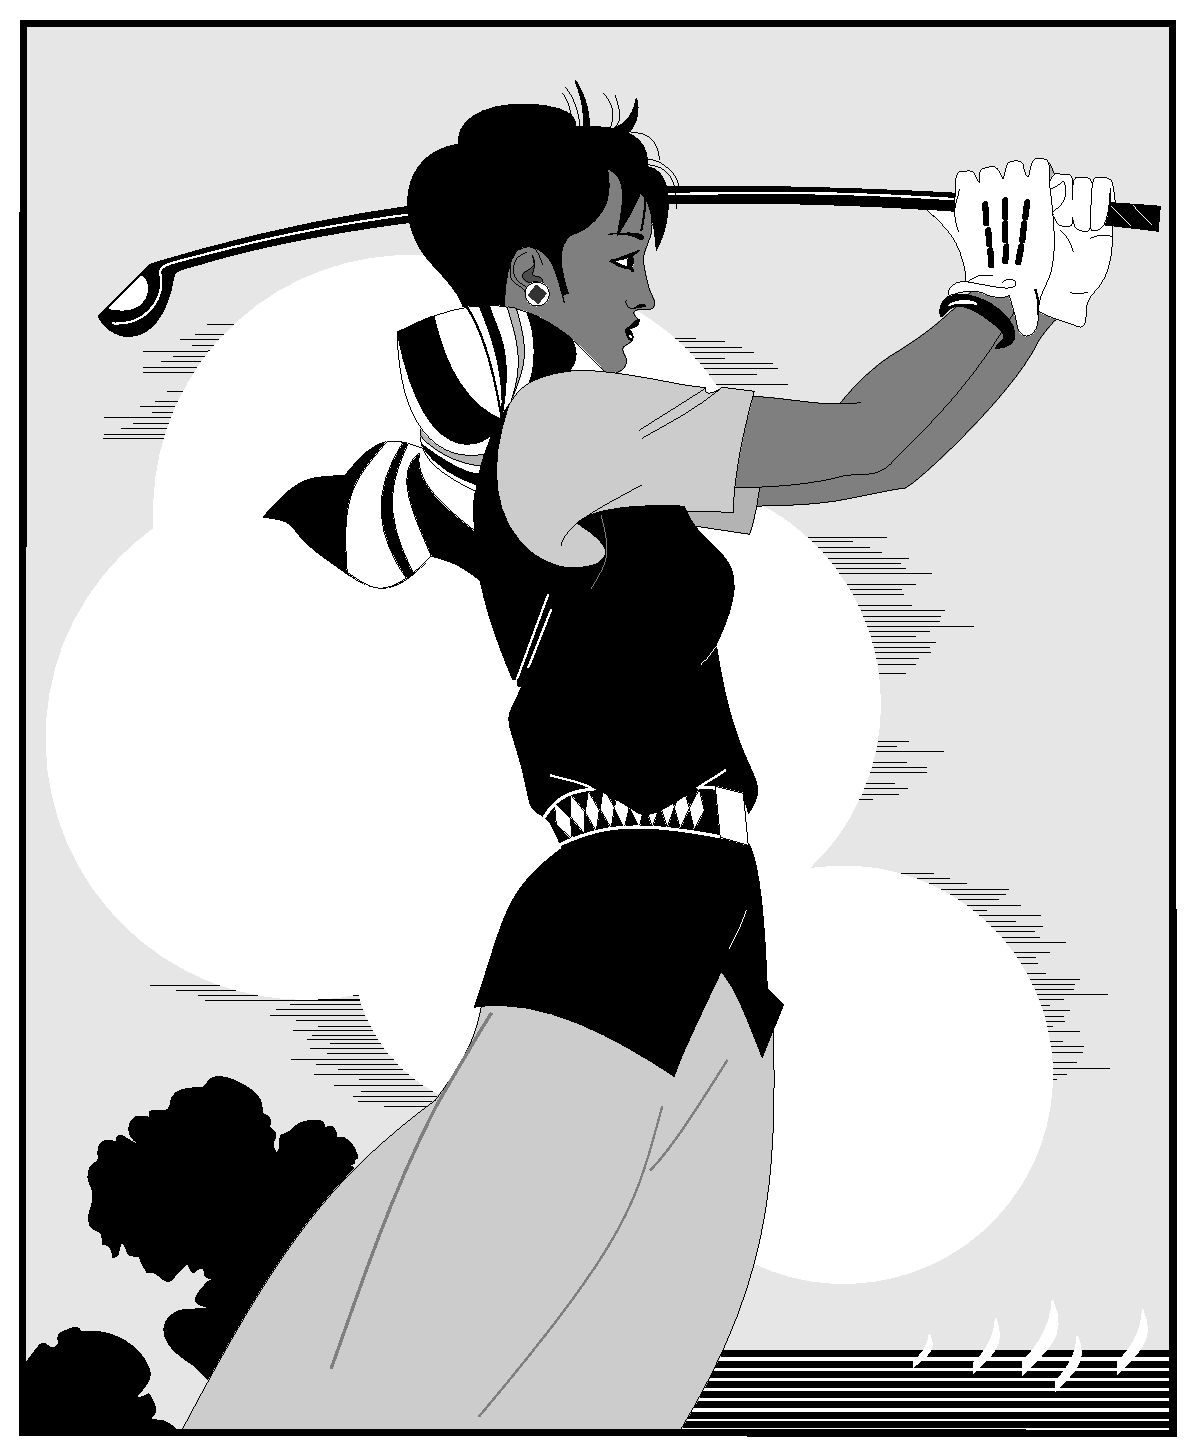
\includegraphics[width = 0.4\textwidth]{golfer}
\bicaption[golfer1]{}{打高尔夫球球的人(博士论文双语题注)}{Fig.$\!$}{The person playing golf (Doctoral thesis)}
\end{figure}

每个图均应有图题(由图序和图名组成),图题不宜有标点符号,图名在图序之后空1个半
角字符排写。图序按章编排,如第1章第一个插图的图号为“图1-1”。图题置于图下,硕士论
文只用中文,博士论文用中、英两种文字,居中书写,中文在上,要求中文用宋体5号字,
英文用Times New Roman 5号字。有图注或其它说明时应置于图题之上。引用图应注明出处
,在图题右上角加引用文献号。图中若有分图时,分图题置于分图之下或图题之下,可以只
用中文书写,分图号用a)、b)等表示。图中各部分说明应采用中文(引用的外文图除外)或
数字符号,各项文字说明置于图题之上(有分图时,置于分图题之上)。图中文字用宋体、
Times New Roman字体,字号尽量采用5号字(当字数较多时可用小5号字,以清晰表达为原
则,但在一个插图内字号要统一)。同一图内使用文字应统一。图表中物理量、符号用斜体
。
\subsection{本硕论文题注}[Other picture example]
\begin{figure}[h]
\centering
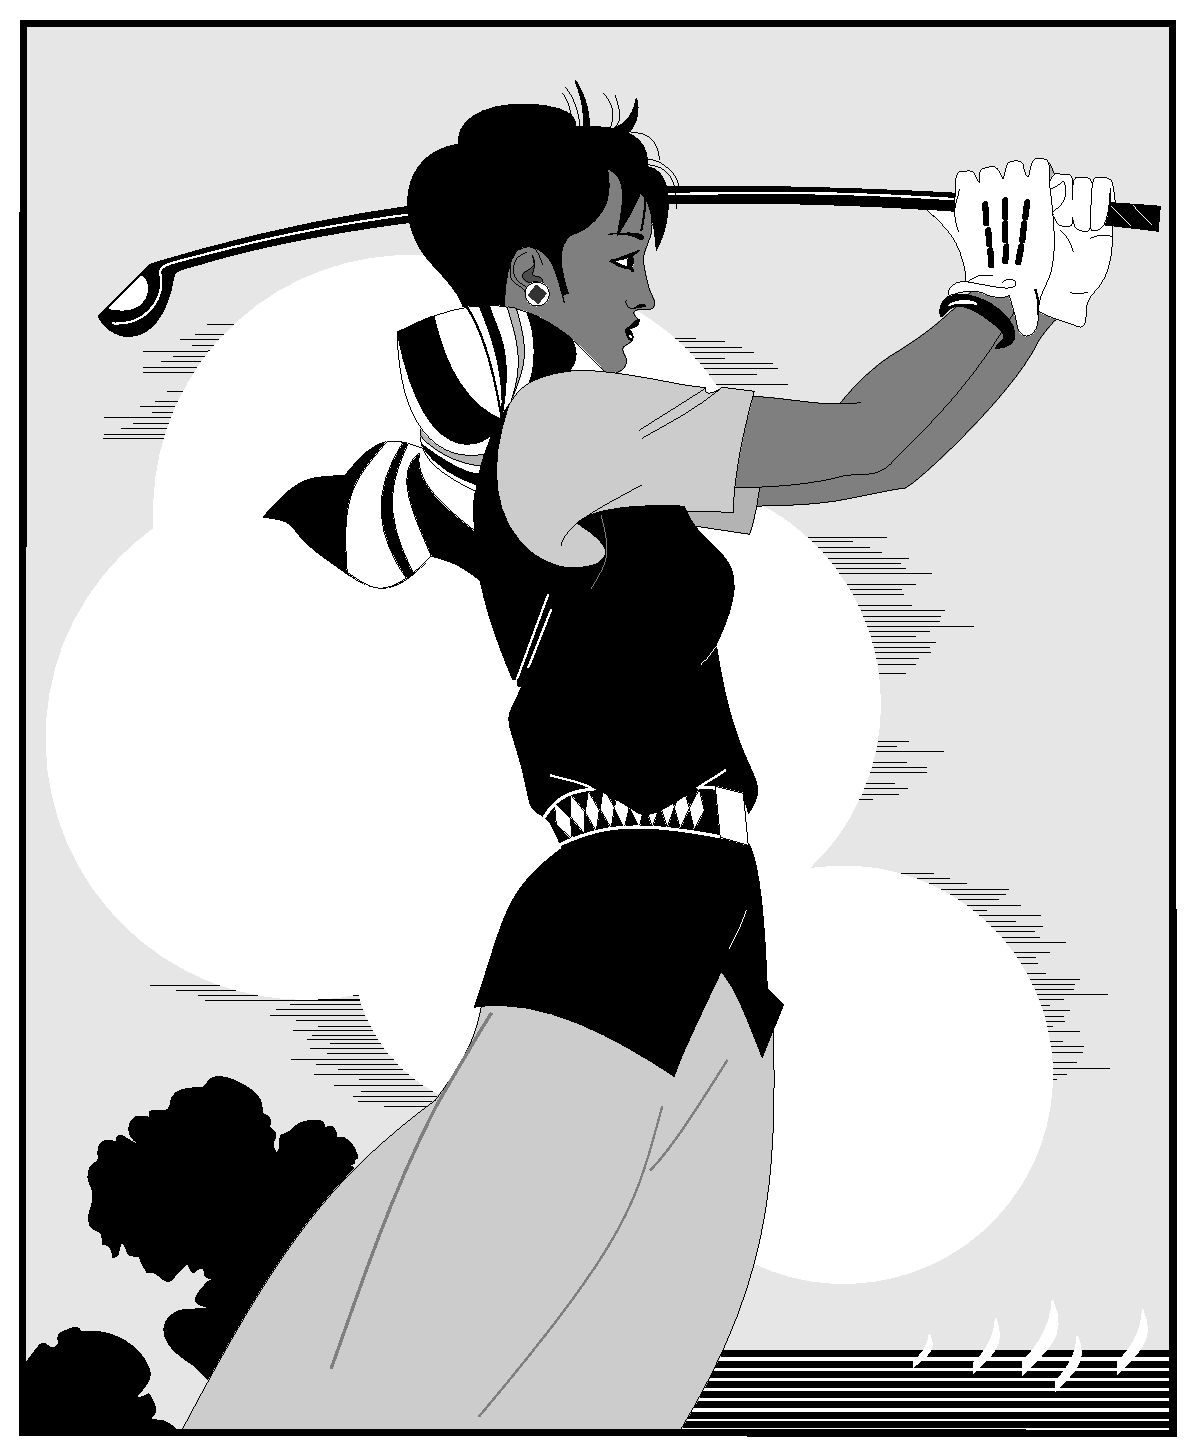
\includegraphics[width = 0.4\textwidth]{golfer}
\caption{打高尔夫球的人,硕士论文要求只用汉语}
\end{figure}

\subsection{并排图和子图}[Abreast-picture and Sub-picture example]
\subsubsection{并排图}[Abreast-picture example]

使用并排图时,需要注意对齐方式。默认情况是中部对齐。这里给出中部对齐、顶部对齐
、图片底部对齐三种常见方式。其中,底部对齐方式有一个很巧妙的方式,将长度比较小
的图放在左面即可。

\begin{figure}[htbp]
\centering
\begin{minipage}{0.4\textwidth}
\centering
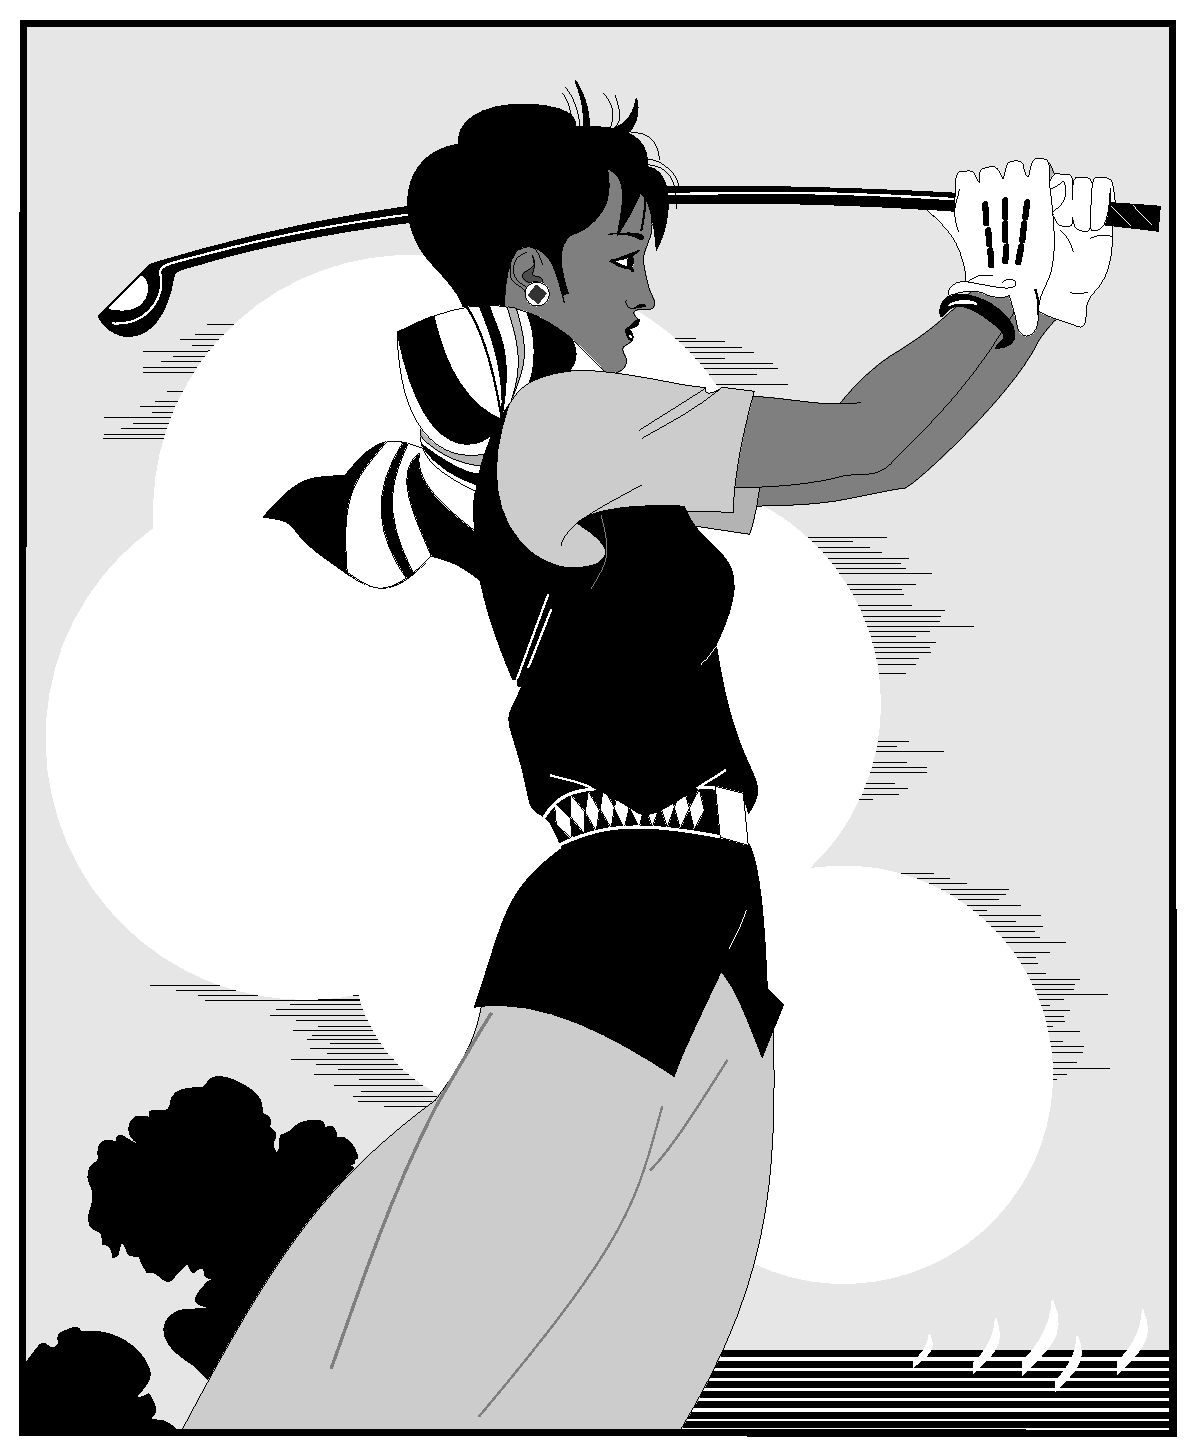
\includegraphics[width=\textwidth]{golfer}
\bicaption[golfer2]{}{打高尔夫球的人}{Fig.$\!$}{The person playing golf}
\end{minipage}
\centering
\begin{minipage}{0.4\textwidth}
\centering
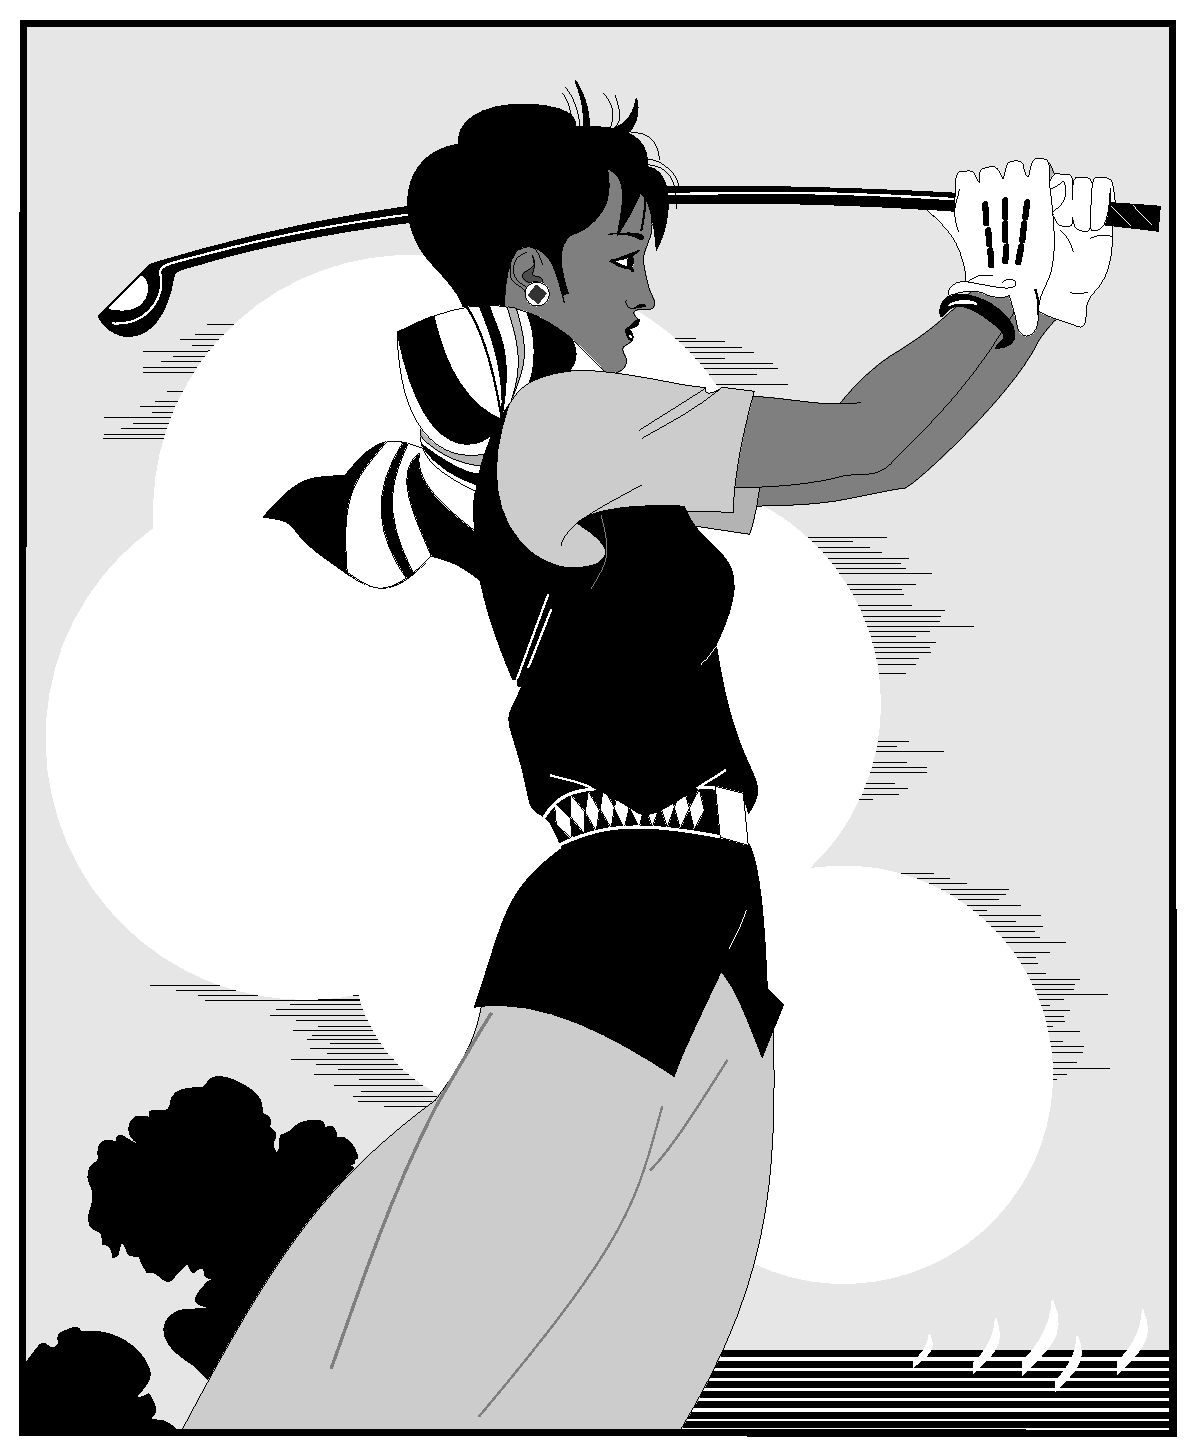
\includegraphics[width=\textwidth]{golfer}
\bicaption[golfer3]{}{打高尔夫球的人。注意,这里默认居中}{Fig.$\!$}{The person playing golf. Please note that, it is vertically center aligned by default.}
\end{minipage}
\end{figure}

\begin{figure}[htbp]
\centering
\begin{minipage}[t]{0.4\textwidth}
\centering
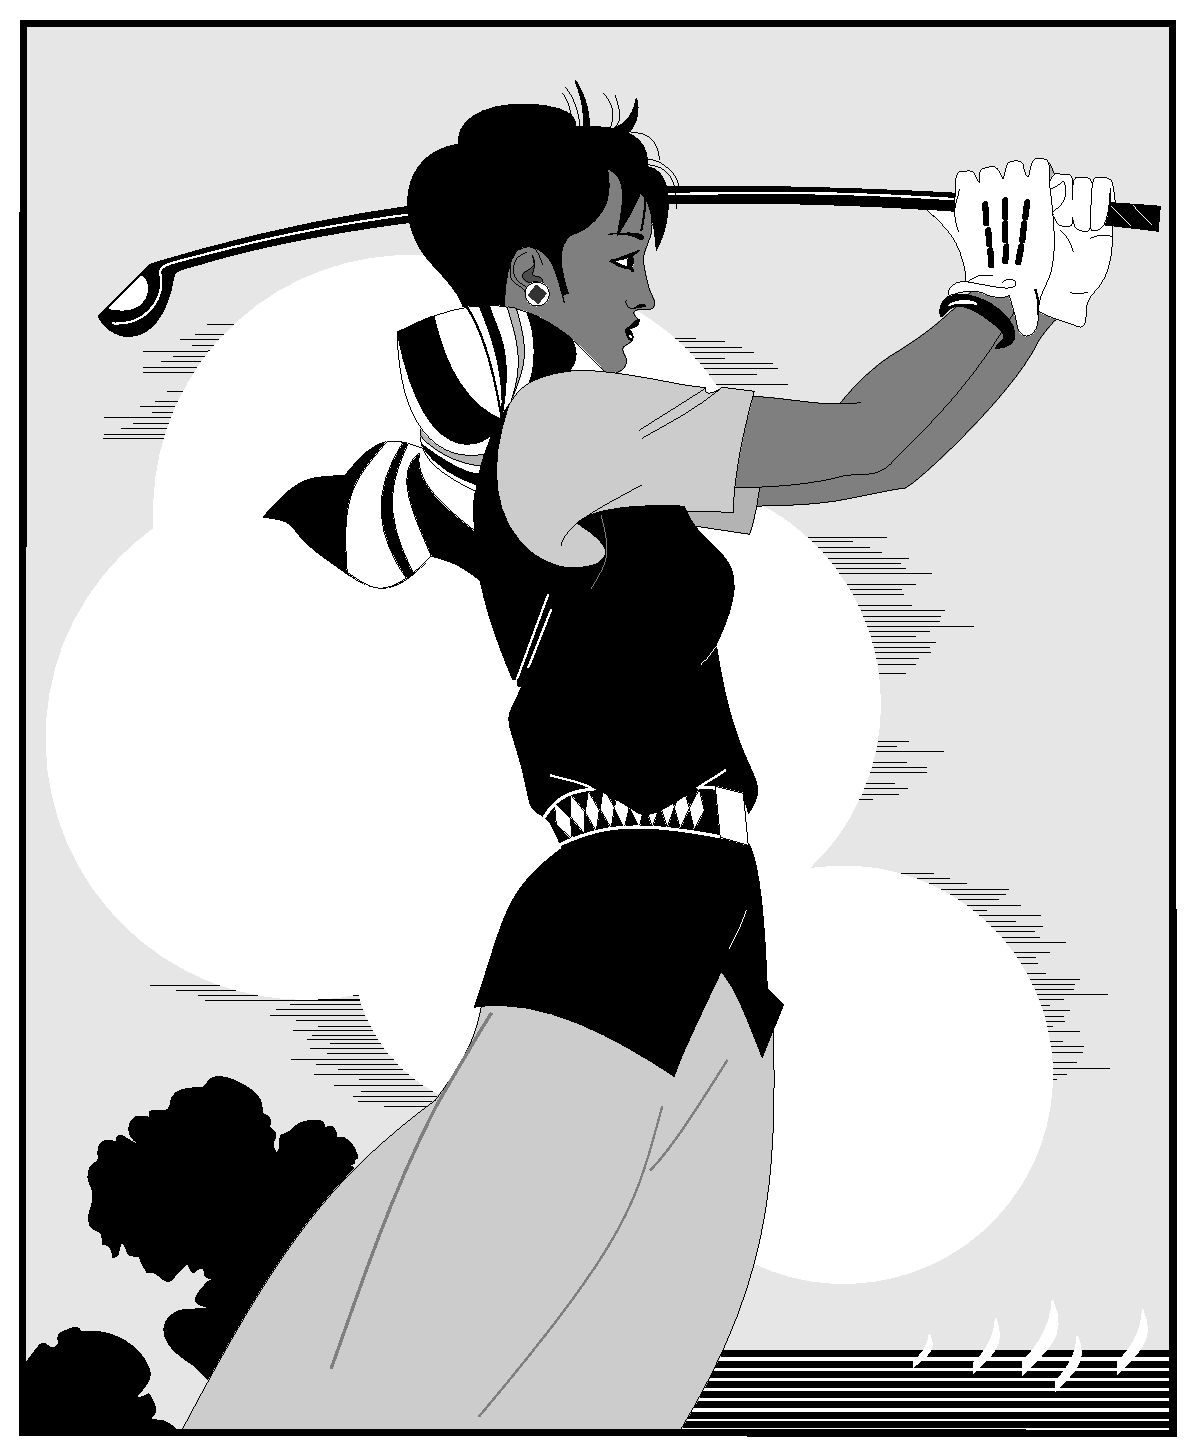
\includegraphics[width=\textwidth]{golfer}
\bicaption[golfer5]{}{打高尔夫球的人}{Fig.$\!$}{The person playing golf}
\end{minipage}
\centering
\begin{minipage}[t]{0.4\textwidth}
\centering
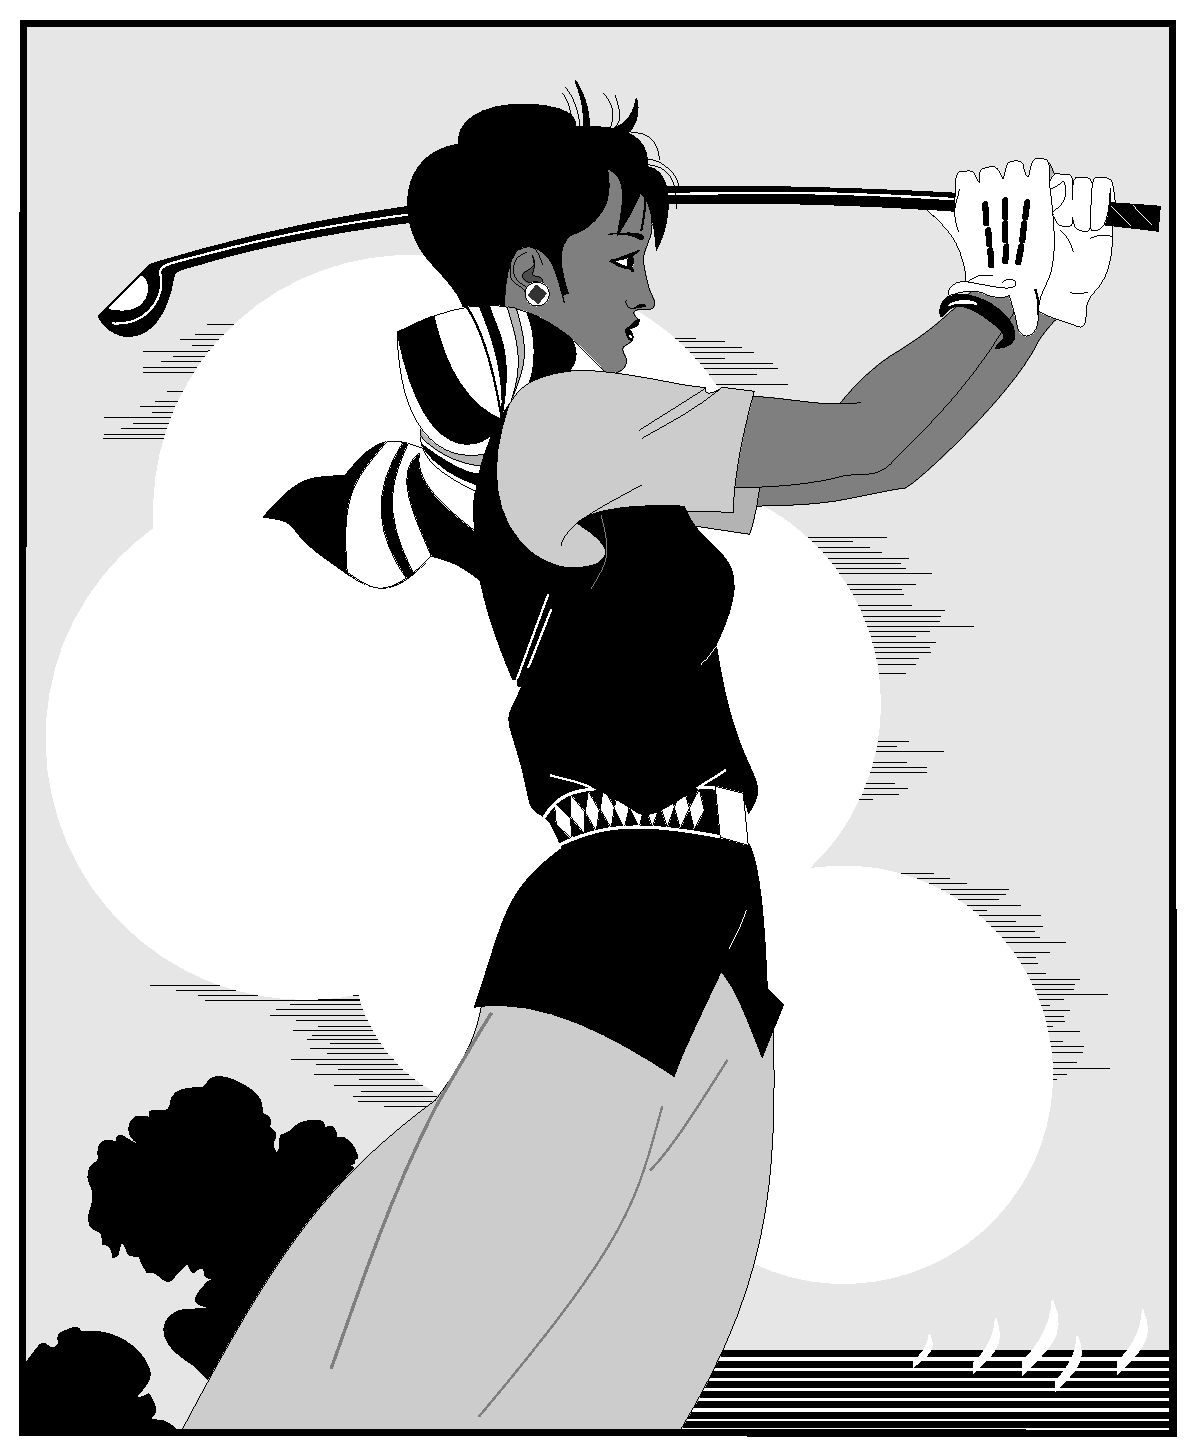
\includegraphics[width=\textwidth]{golfer}
\bicaption[golfer8]{}{打高尔夫球的人。注意,此图是顶部对齐}{Fig.$\!$}{The person playing golf. Please note that, it is vertically top aligned.}
\end{minipage}
\end{figure}

\begin{figure}[htbp]
\centering
\begin{minipage}[t]{0.4\textwidth}
\centering
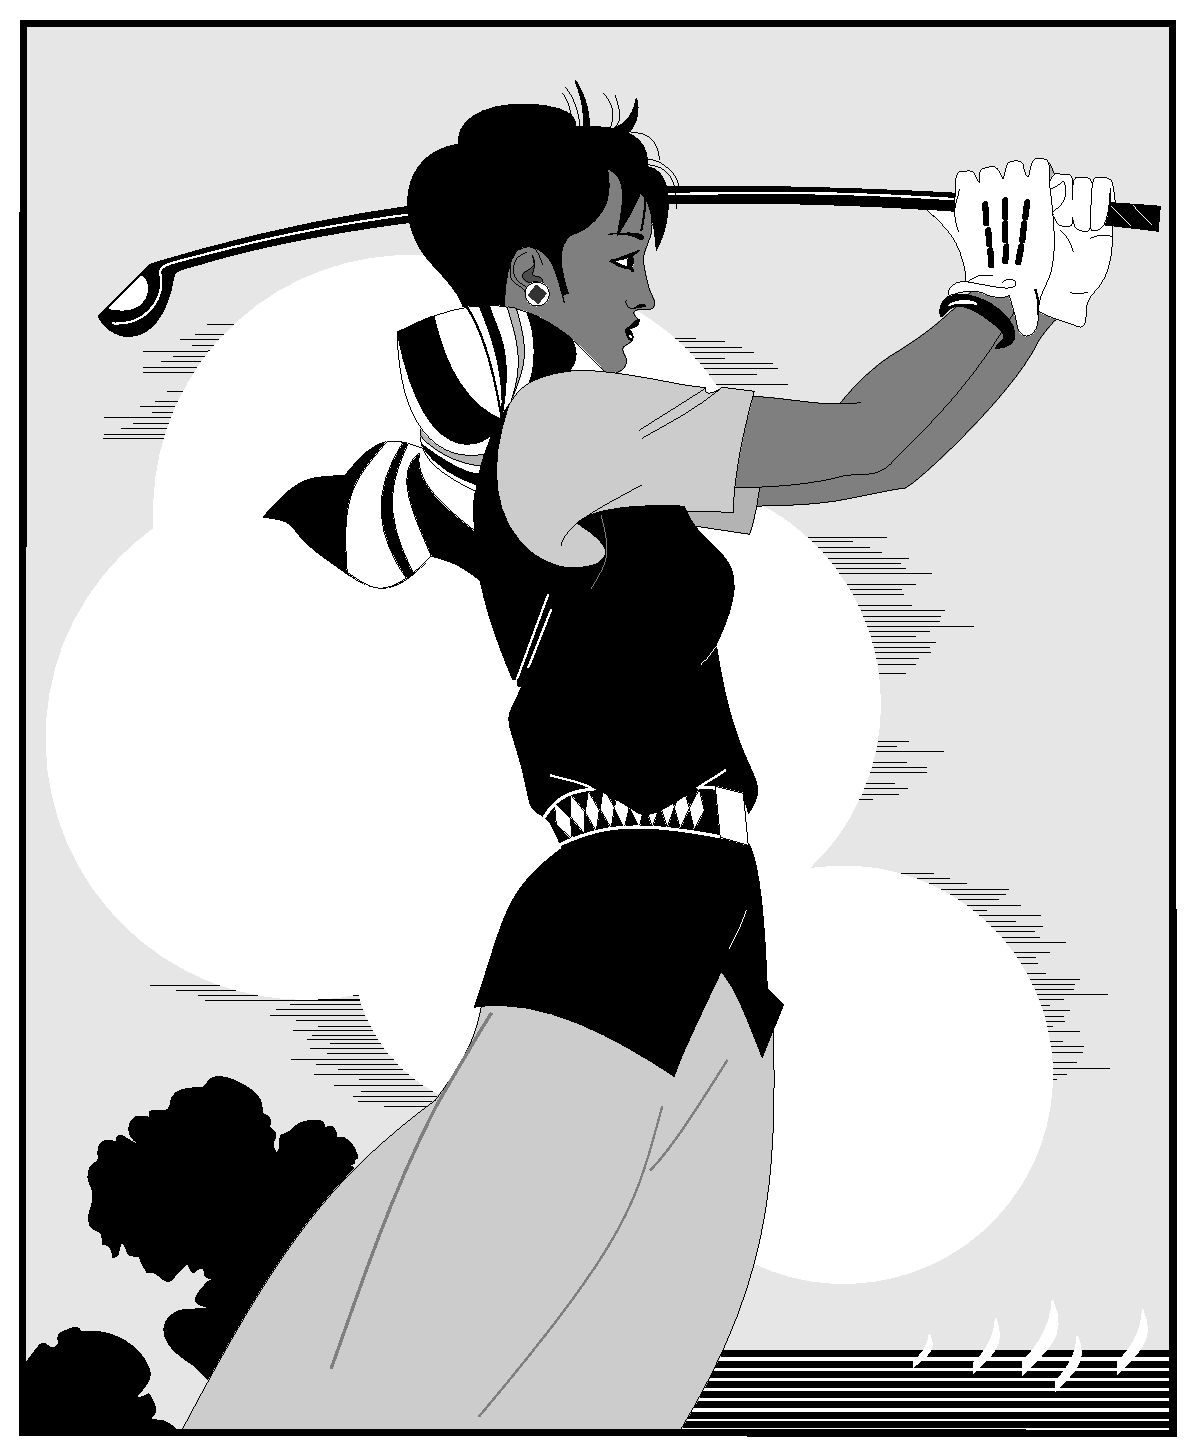
\includegraphics[width=\textwidth,height=\textwidth]{golfer}
\bicaption[golfer9]{}{打高尔夫球的人。注意,此图对齐方式是图片底部对齐}{Fig.$\!$}{The person playing golf. Please note that, it is vertically bottom aligned for figure.}
\end{minipage}
\centering
\begin{minipage}[t]{0.4\textwidth}
\centering
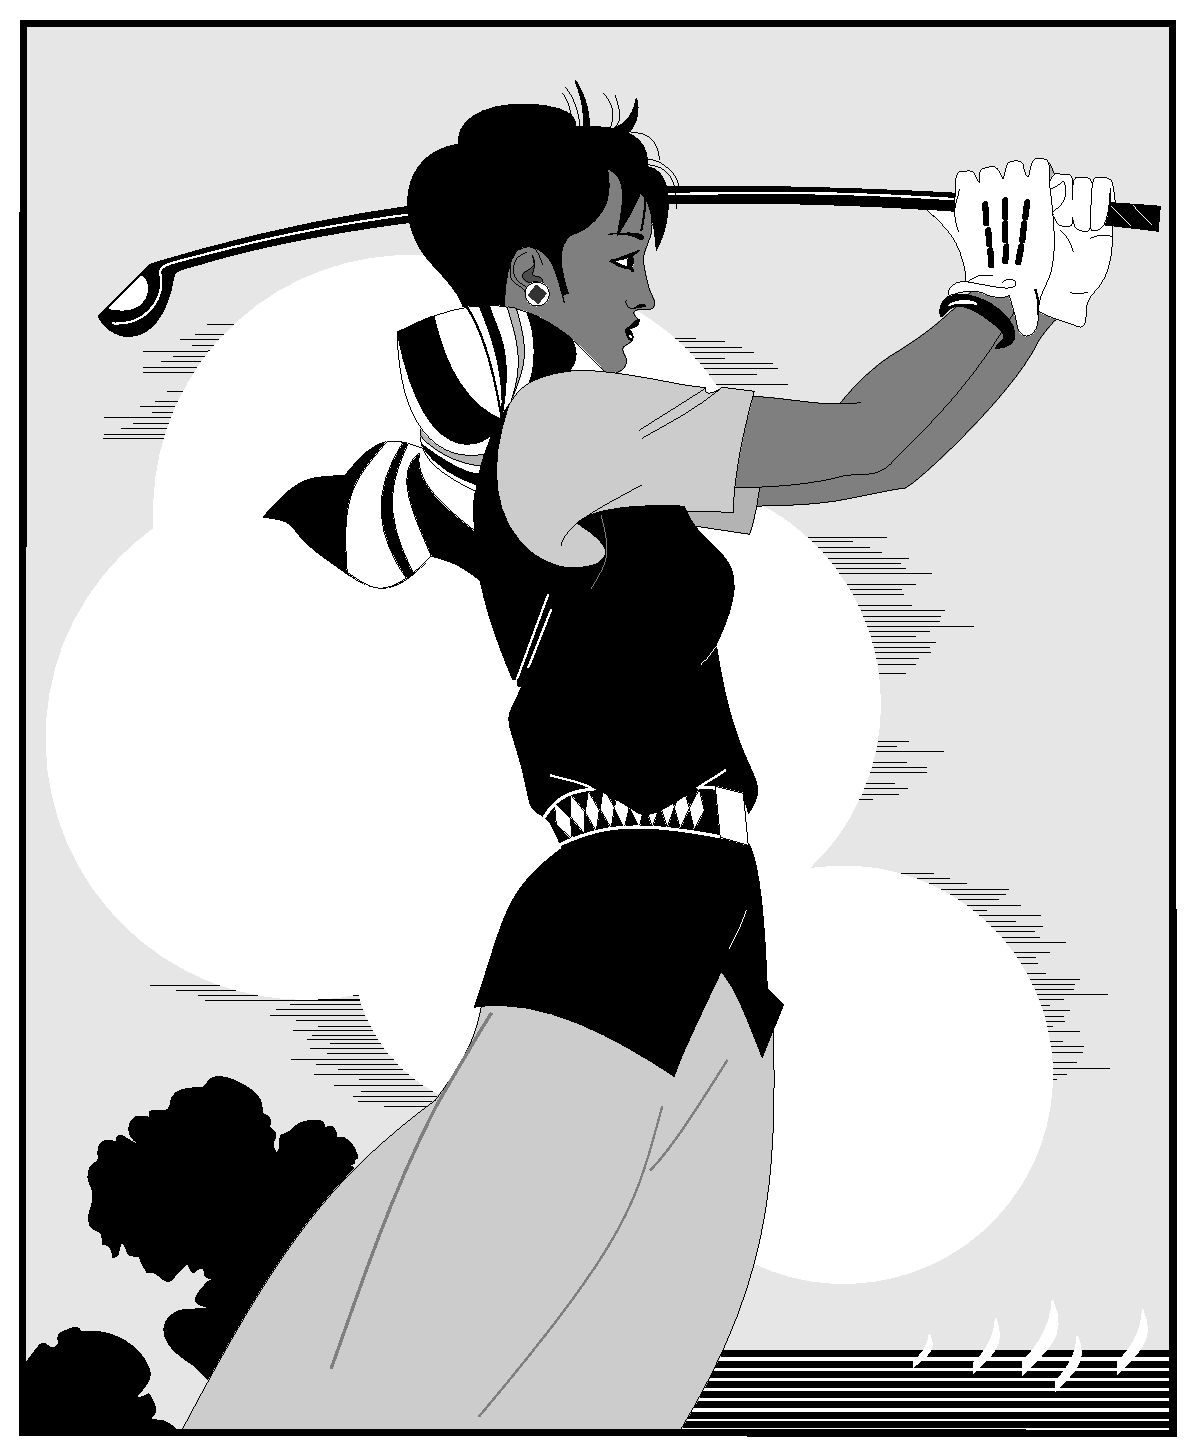
\includegraphics[width=\textwidth]{golfer}
\bicaption[golfer6]{}{打高尔夫球的人}{Fig.$\!$}{The person playing golf}
\end{minipage}
\end{figure}

\subsubsection{子图}[Sub-picture example]
注意:子图题注也可以只用中文。规范规定“分图题置于分图之下或图题之下”,但没有给出具体的格式要求。
没有要求的另外一个说法就是“无论什么格式都不对”。
所以只有在一个图中有标注“a),b)”,无法使用\cs{subfigure}的情况下,使用最后一个图例中的格式设置方法,否则不要使用。
为了应对“无论什么格式都不对”,这个子图图题使用“minipage”和“description”环境,宽度,对齐方式可以按照个人喜好自由设置,是否使用双语子图图题也可以自由设置。

\begin{figure}[!h]
\setlength{\subfigcapskip}{-1bp}
\centering
\begin{minipage}{\textwidth}
\centering
\subfigure{\label{golfer41}}\addtocounter{subfigure}{-2}
\subfigure[The person playing golf]{\subfigure[打高尔夫球的人~1]{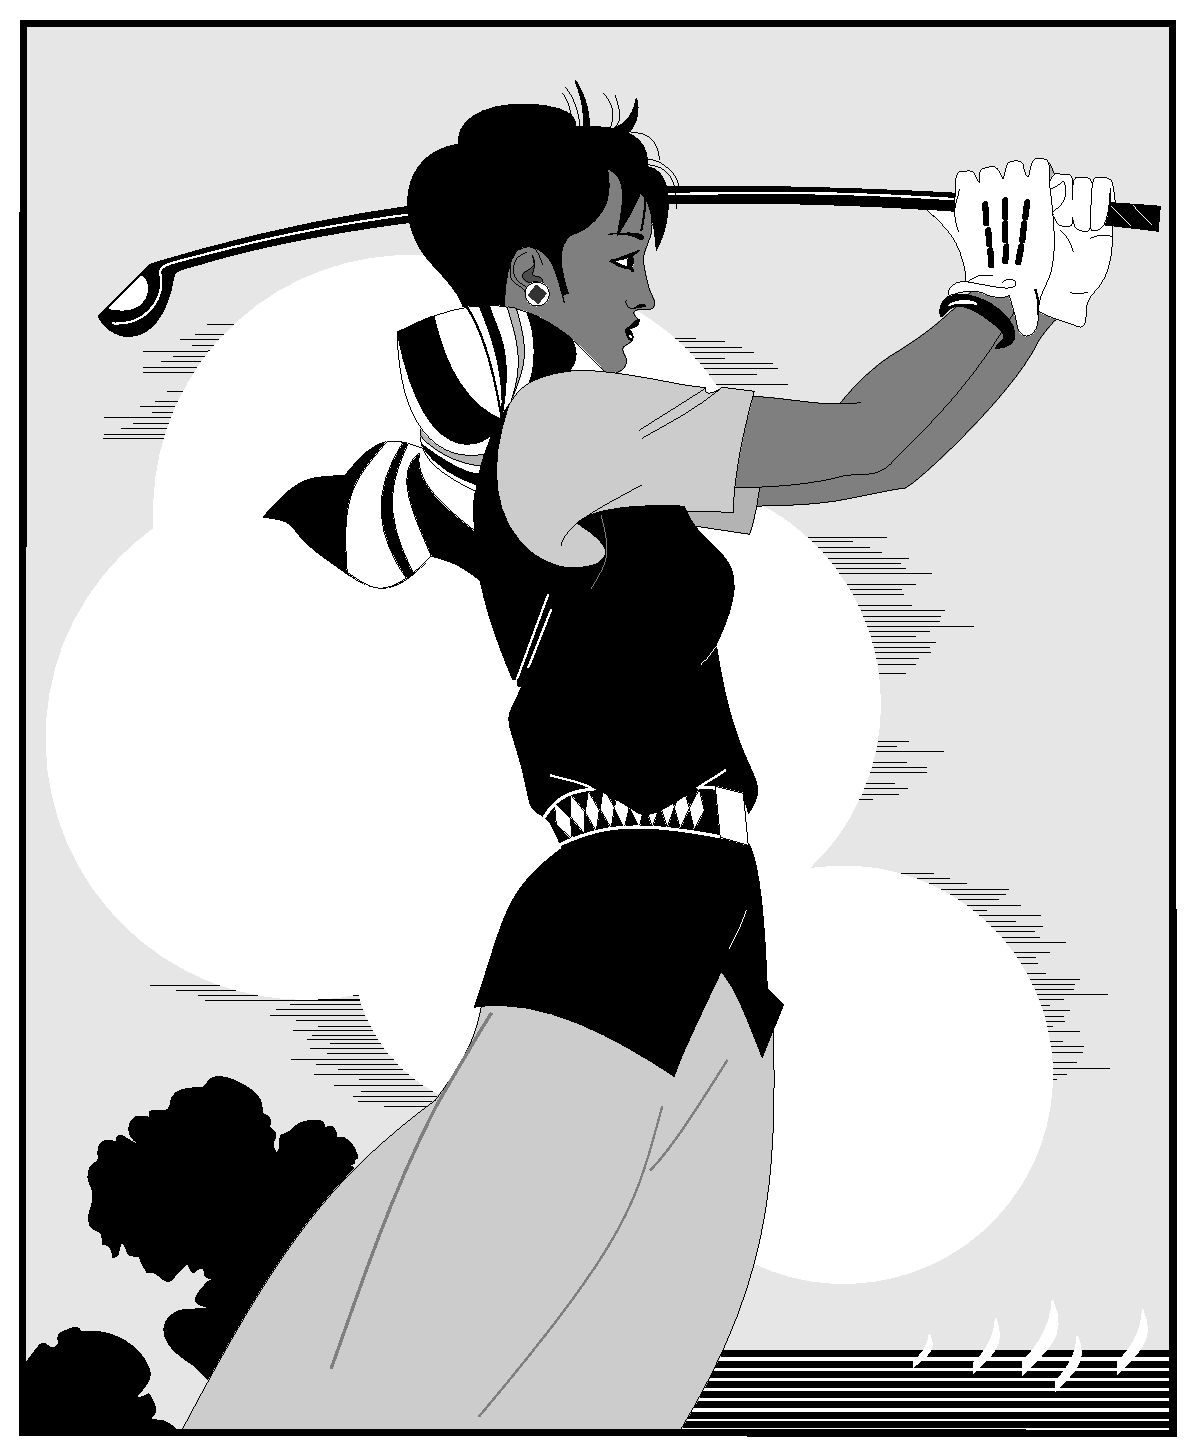
\includegraphics[width=0.4\textwidth]{golfer}}}
\hspace{2em}
\subfigure{\label{golfer42}}\addtocounter{subfigure}{-2}
\subfigure[The person playing golf]{\subfigure[打高尔夫球的人~2]{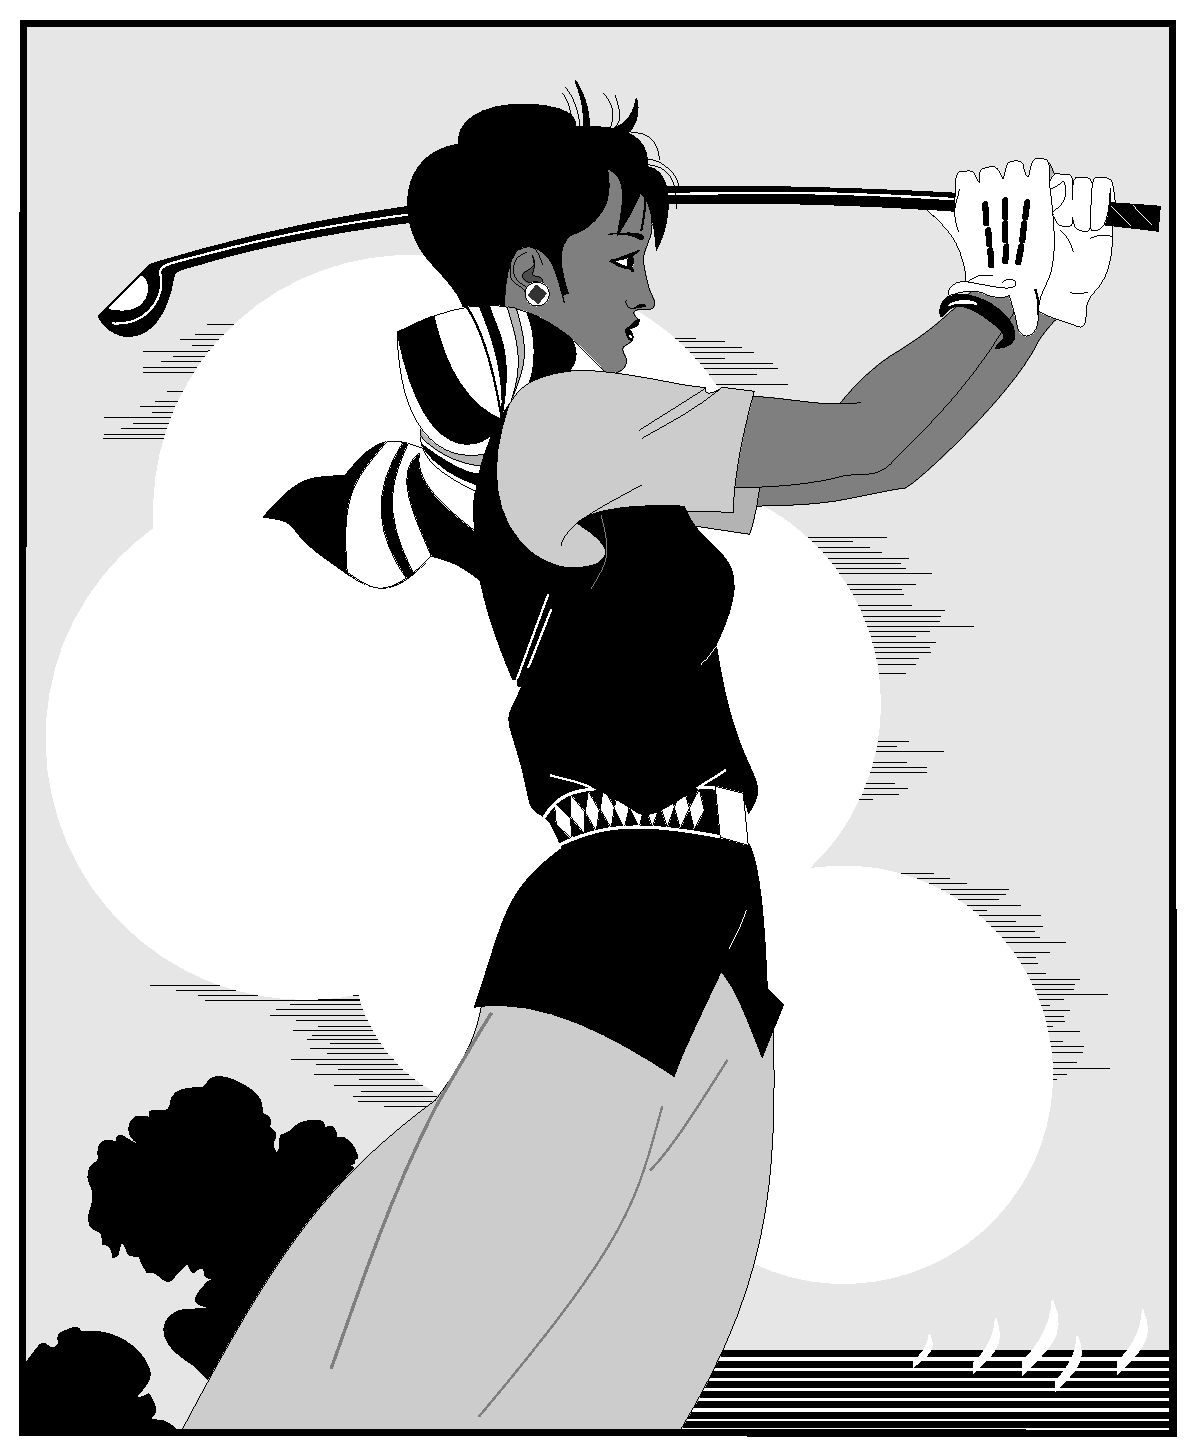
\includegraphics[width=0.4\textwidth]{golfer}}}
\end{minipage}
\centering
\begin{minipage}{\textwidth}
\centering
\subfigure{\label{golfer43}}\addtocounter{subfigure}{-2}
\subfigure[The person playing golf]{\subfigure[打高尔夫球的人~3]{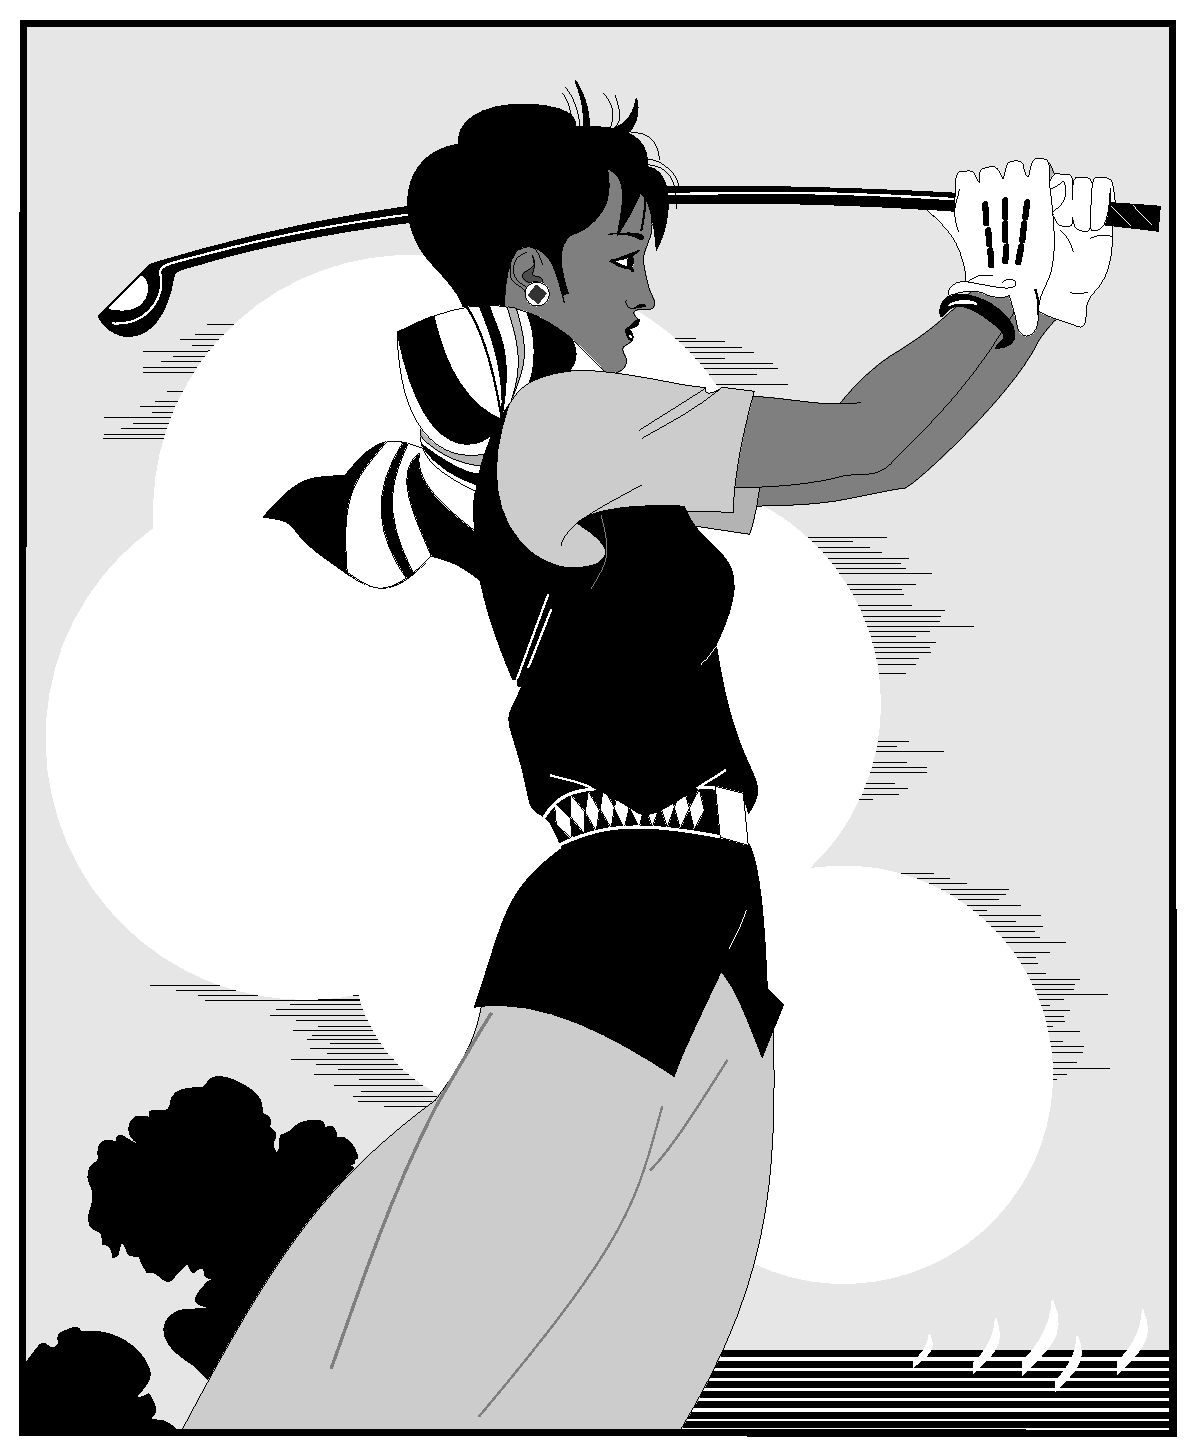
\includegraphics[width=0.4\textwidth]{golfer}}}
\hspace{2em}
\subfigure{\label{golfer44}}\addtocounter{subfigure}{-2}
\subfigure[The person playing golf. Here, 'hang indent' and 'center last line' are not stipulated in the regulation.]{\subfigure[打高尔夫球的人~4。注意,规范中没有明确规定要悬挂缩进、最后一行居中。]{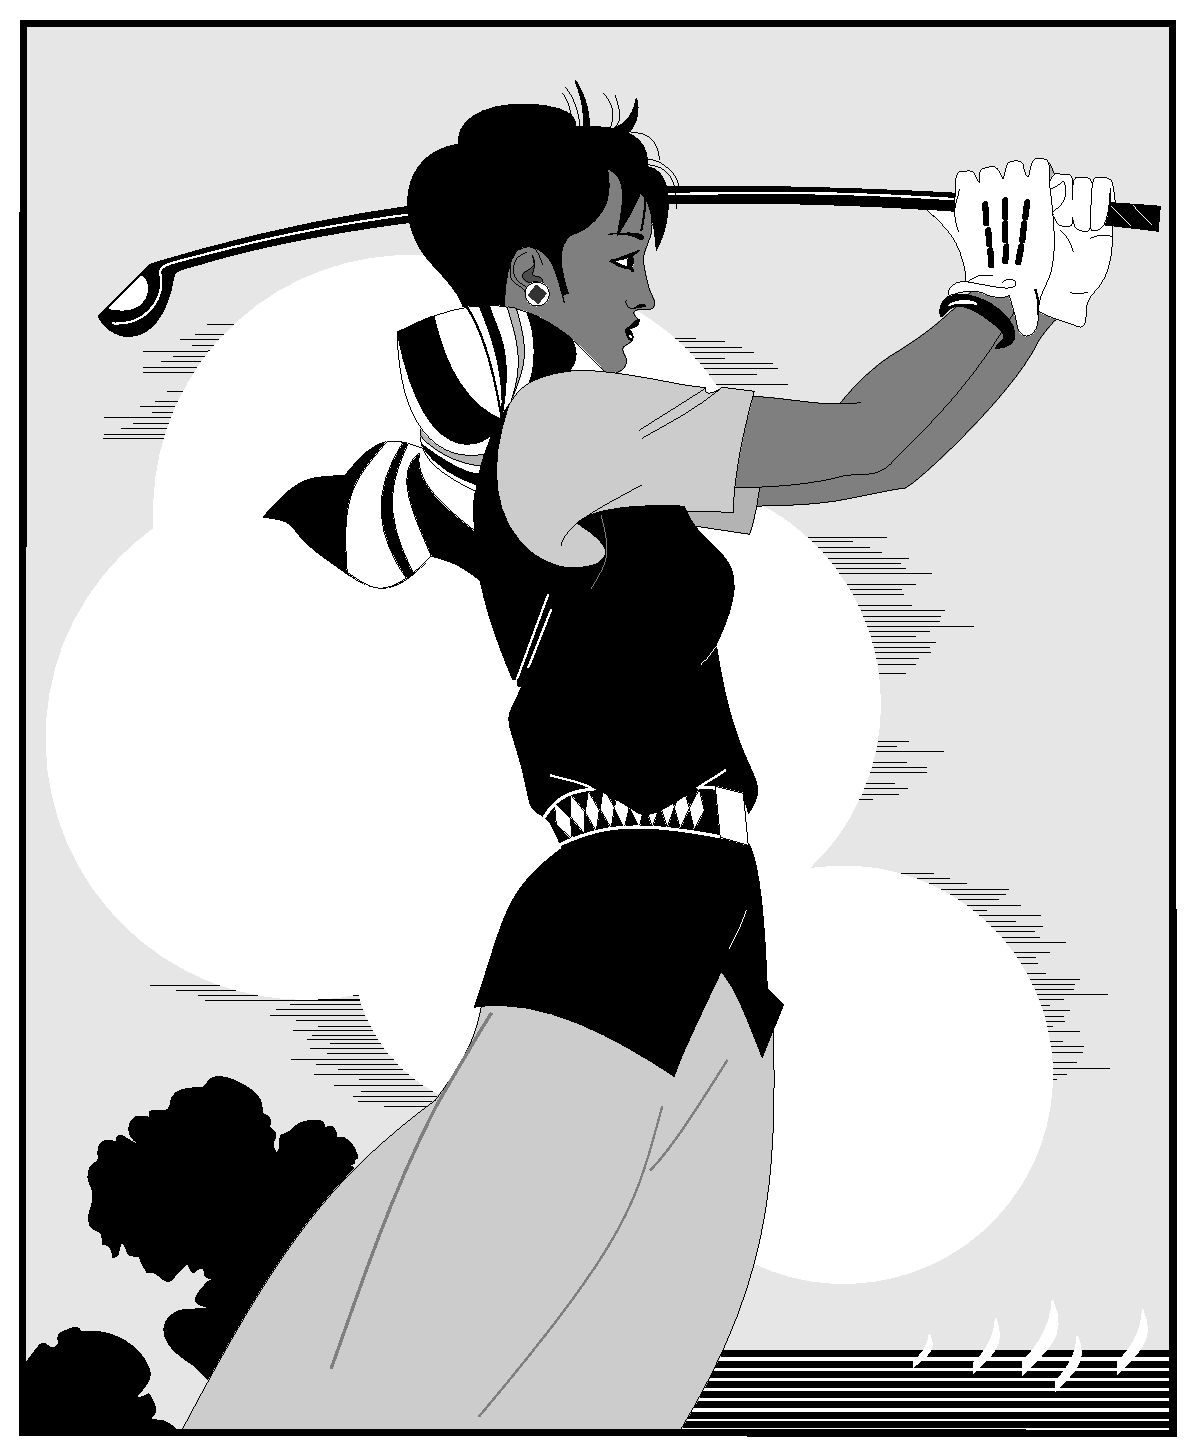
\includegraphics[width=0.4\textwidth]{golfer}}}
\end{minipage}
\vspace{0.2em}
\bicaption[golfer4]{}{打高尔夫球的人}{Fig.$\!$}{The person playing gol}
\end{figure}

\begin{figure}[t]
  \centering
  \begin{minipage}{.7\linewidth}
    \setlength{\subfigcapskip}{-1bp}
    \centering
    \begin{minipage}{\textwidth}
      \centering
      \subfigure{\label{golfer45}}\addtocounter{subfigure}{-2}
      \subfigure[The person playing golf]{\subfigure[打高尔夫球的人~1]{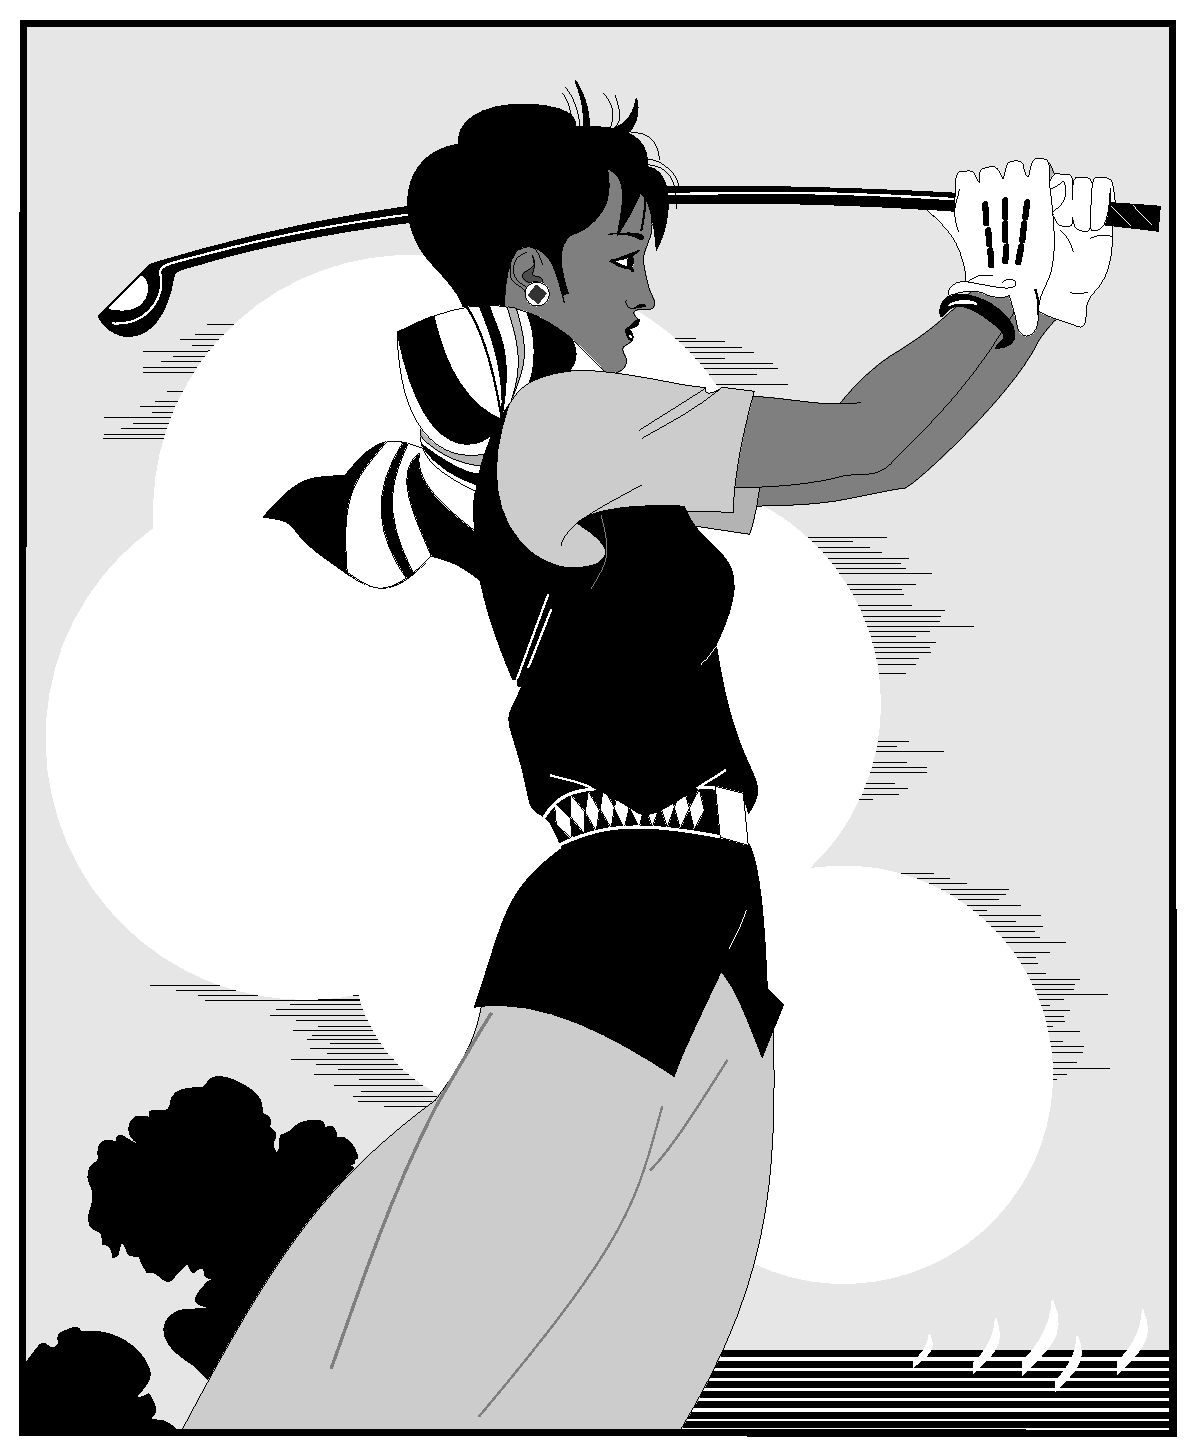
\includegraphics[width=0.4\textwidth]{golfer}}}
      \hspace{4em}
      \subfigure{\label{golfer46}}\addtocounter{subfigure}{-2}
      \subfigure[The person playing golf]{\subfigure[打高尔夫球的人~2]{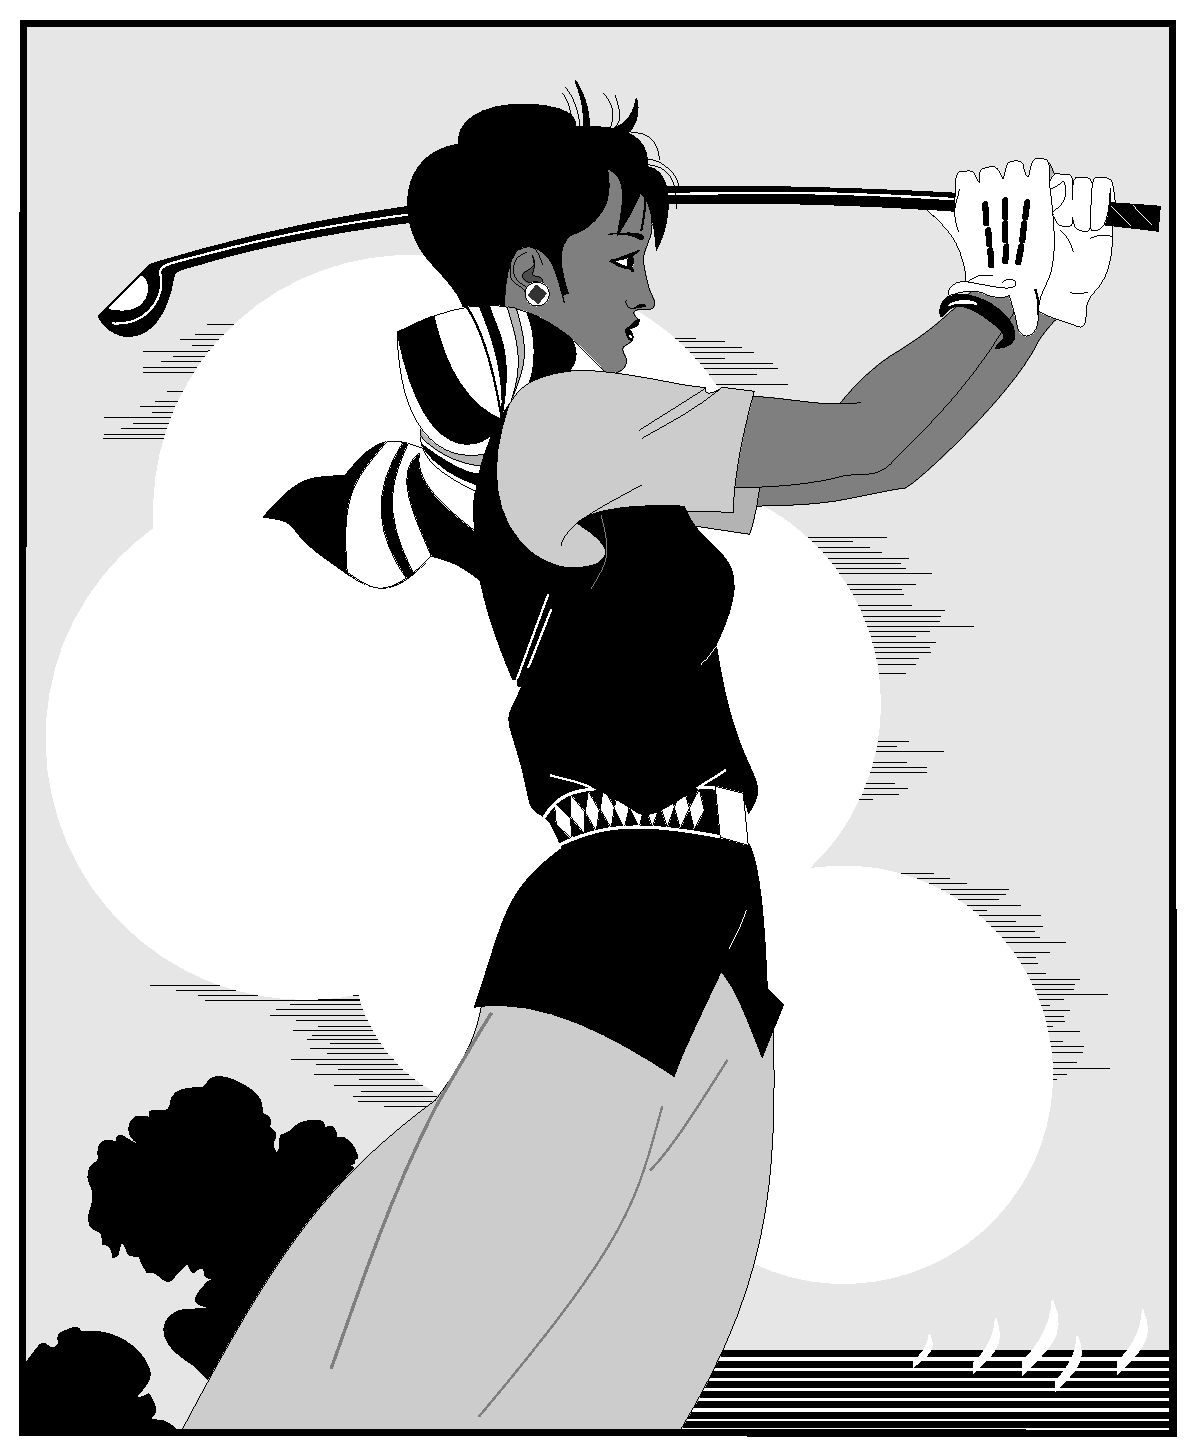
\includegraphics[width=0.4\textwidth]{golfer}}}
    \end{minipage}
    \vskip 0.2em
  \wuhao 注意:这里是中文图注添加位置(我工要求,图注在图题之上)。
    \vspace{0.2em}
\bicaption[golfer47]{}{打高尔夫球的人。注意,此处我工有另外一处要求,子图图题可以位于主图题之下。但由于没有明确说明位于下方具体是什么格式,所以这里不给出举例。}{Fig.$\!$}{The person playing golf. Please note that, although it is appropriate to put subfigures' captions under this caption as stipulated in regulation, but its format is not clearly stated.}
  \end{minipage}
\end{figure}

\begin{figure}[t]
\centering
\begin{tikzpicture}
	\node[anchor=south west,inner sep=0] (image) at (0,0) {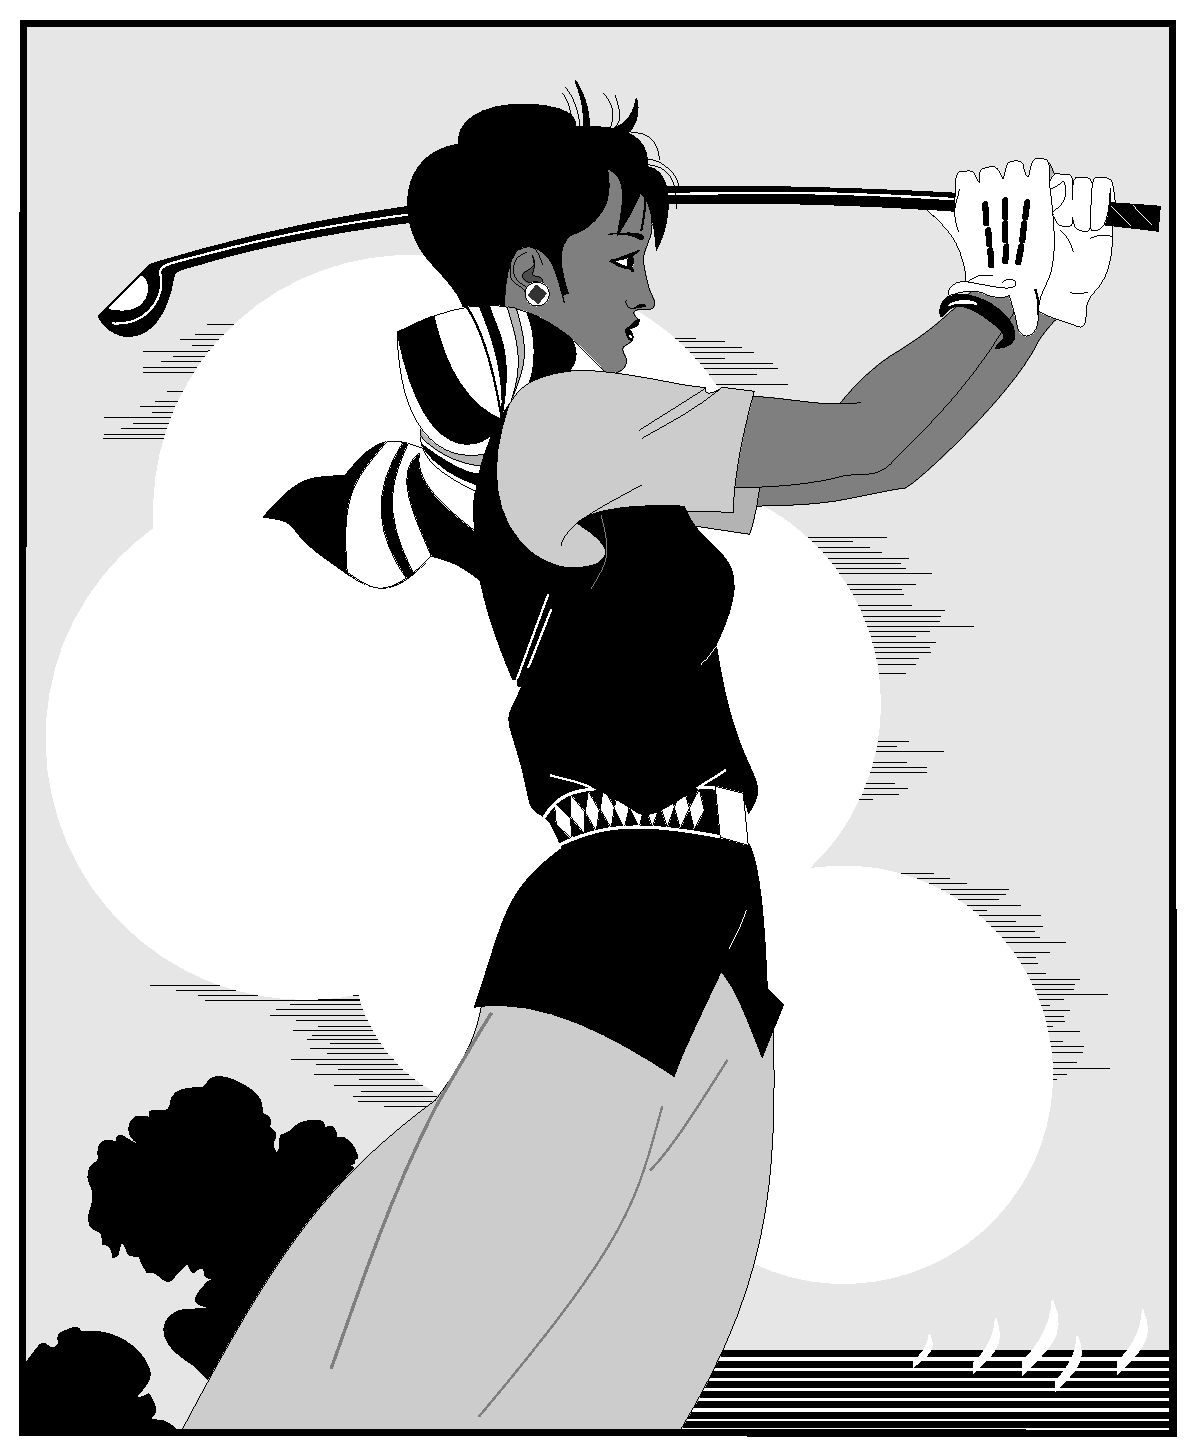
\includegraphics[width=0.3\textwidth]{golfer}};
	\begin{scope}[x={(image.south east)},y={(image.north west)}]
		\node at (0.3,0.5) {a)};
		\node at (0.8,0.2) {b)};
	\end{scope}
\end{tikzpicture}
\bicaption[golfer0]{}{打高尔夫球球的人(博士论文双语题注)}{Fig.$\!$}{The person playing golf (Doctoral thesis)}
\vskip -0.4em
 \hspace{2em}
\begin{minipage}[t]{0.3\textwidth}
\wuhao \setlist[description]{font=\normalfont}
	\begin{description}
		\item[(a)]子图图题
	\end{description}
 \end{minipage}
 \hspace{2em}
 \begin{minipage}[t]{0.3\textwidth}
\wuhao \setlist[description]{font=\normalfont}
	\begin{description}
		\item[(b)]子图图题
		\item[(b)]Subfigure caption
	\end{description}
\end{minipage}
\end{figure}


\begin{figure}[!h]
	\centering
	\begin{sideways}
		\begin{minipage}{\textheight}
			\centering
			\fbox{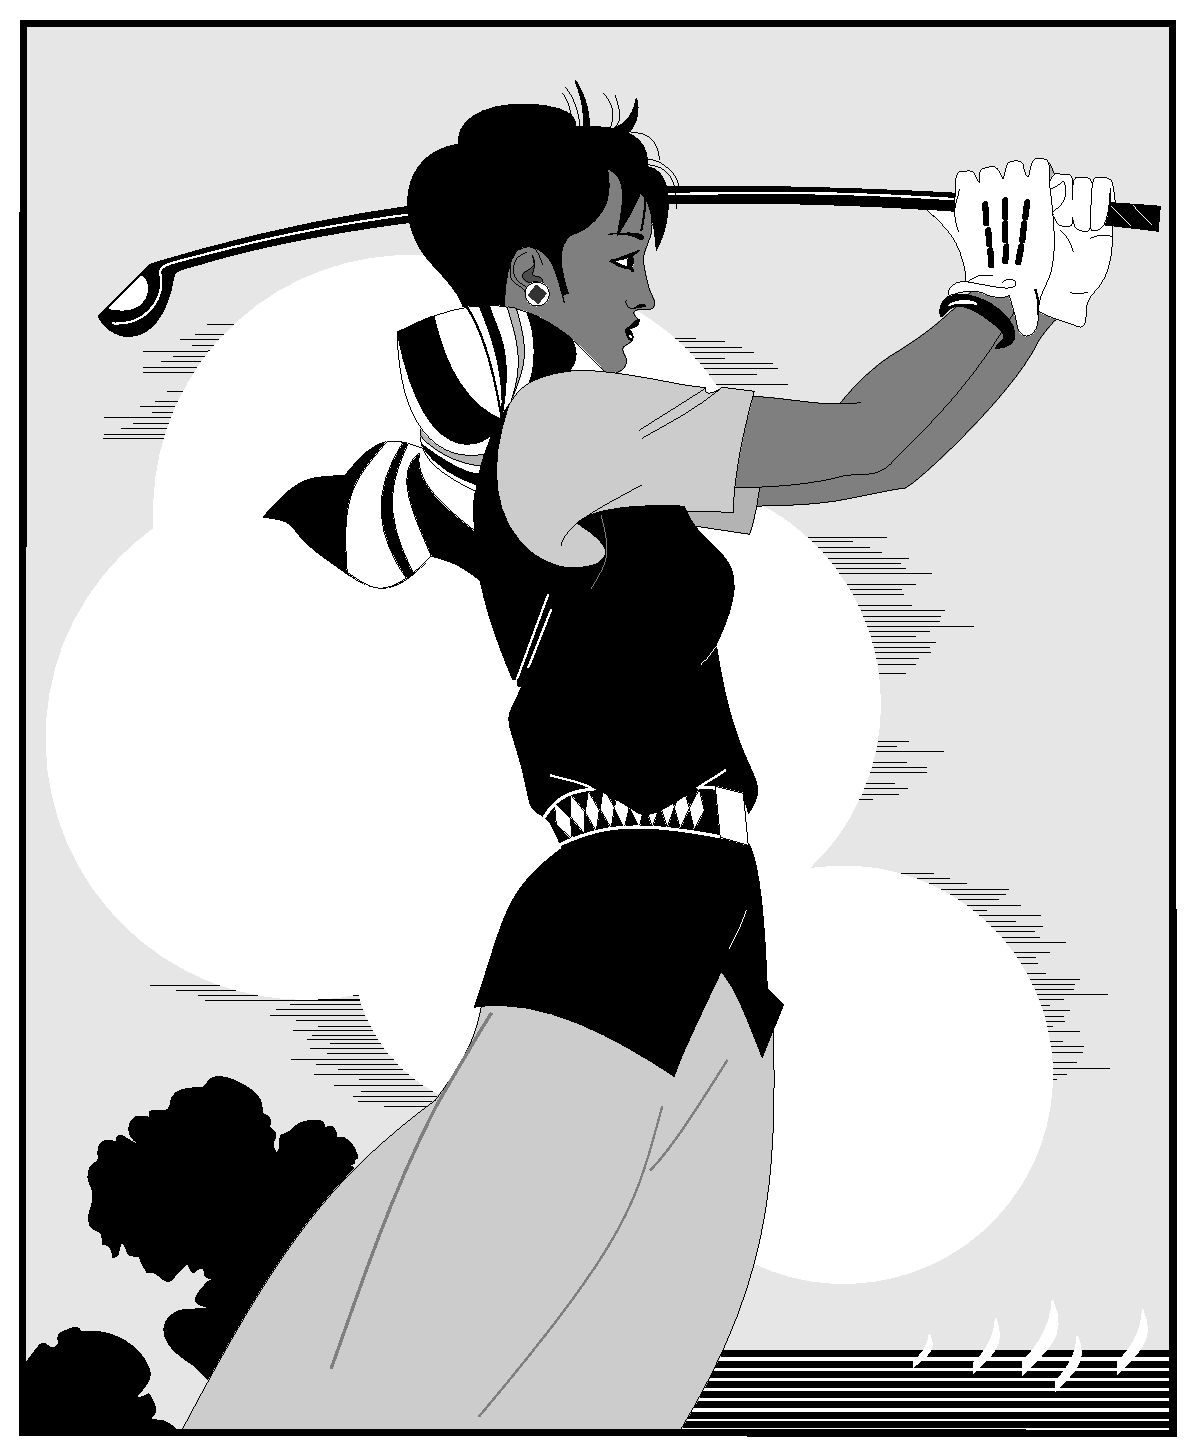
\includegraphics[width=0.2\textwidth]{golfer}}
			\fbox{\includegraphics[width=0.2\textwidth]{golfer}}
			\fbox{\includegraphics[width=0.2\textwidth]{golfer}}
			\fbox{\includegraphics[width=0.2\textwidth]{golfer}}
			\fbox{\includegraphics[width=0.2\textwidth]{golfer}}
			\fbox{\includegraphics[width=0.2\textwidth]{golfer}}
			\fbox{\includegraphics[width=0.2\textwidth]{golfer}}
\bicaption[golfer7]{}{打高尔夫球的人(非规范要求)}{Fig.$\!$}{The person playing golf (Not stated in the regulation)}
		\end{minipage}
	\end{sideways}
\end{figure}

\clearpage

如果不想让图片浮动到下一章节,那么在此处使用\cs{clearpage}命令。

\section{如何做出符合规范的漂亮的图}
关于作图工具在后文\ref{drawtool}中给出一些作图工具的介绍,此处不多言。
此处以R语言和Tikz为例说明如何做出符合规范的图。

\subsection{Tikz作图举例}
使用Tikz作图核心思想是把格式、主题、样式与内容分离,定义在全局中。
注意字体设置可以有两种选择,如何字少,用五号字,字多用小五。
使用Tikz作图不会出现字体问题,字体会自动与正文一致。

\begin{figure}[thb!]
  \centering
      \begin{tikzpicture}[xscale=0.8,yscale=0.3,rotate=90]
        \small
	\draw (-22,6.5) node[refcell]{参考基因组};
	\draw[refline] (-23, 5) -- (27, 5);
	\draw (-22,3.75) node[tscell]{肿瘤样本};
	\draw (-20,3.75) node[tncell]{正常细胞};
	\draw[tnline] (-21, 2.5) -- (27, 2.5);
	\draw (-20,1.25) node[ttcell]{肿瘤细胞};
	\rcell{2}{6};
	\draw[fakeevolve] (4.5, 5.25) -- (4.5, 4.8);
	\ncell{2}{4};
	\draw[evolve] (4.5, 3) .. controls (4.5,2.8) and (-3.5,2.9) ..  (-3.5, 2);
	\draw[evolve] (4.5, 3) .. controls (4.5,2.8) and (11.5,2.9) .. (11.5, 2);
	\tcellone{-6}{1.5};
	\draw (-9, 2) node[ttcell]{1};
	\draw[evolve] (-3.5, 0) .. controls (-3.5,-0.2) and (-12,-0.1) .. (-12, -1.5);
	\draw[evolve] (-3.5, 0) .. controls (-3.5,-0.2) and (1.5,-0.1) .. (1.5, -1.5);
	\tcellthree{7}{1.5};
	\draw (4, 2) node[ttcell]{2};
	\draw[evolve] (11, 0.5) .. controls (11,0.3) and (19,0.4) .. (19, -1.5);
	\tcellfive{-16}{-2};
	\draw (-19, -1.5) node[ttcell]{3};
	\tcelltwo{-1}{-2};
	\draw (-4, -1.5) node[ttcell]{4};
	\tcellfour{12}{-2};
	\draw (9, -1.5) node[ttcell]{5};
      \end{tikzpicture}
  \begin{minipage}{.9\linewidth}
      \vskip 0.2em
      \wuhao 图中,带有箭头的淡蓝色箭头表示肿瘤子种群的进化方向。一般地,从肿瘤组织中取用于进行二代测序的样本中含有一定程度的正常细胞污染,因此肿瘤的样本中含有正常细胞和肿瘤细胞。每一个子种群的基因组的模拟过程是把生殖细胞变异和体细胞变异加入到参考基因组中。
      \vspace{0.6em}
  \end{minipage}
\bicaption[tumor]{}{肿瘤组织中各个子种群的进化示意图}{Fig.$\!$}{The diagram of tumor subpopulation evolution process}
\end{figure}

\subsection{R作图}
R是一种极具有代表性的典型的作图工具,应用广泛。
与Tikz图~\ref{tumor}~不同,R作图分两种情况:(1)可以转换为Tikz码;(2)不可转换为Tikz码。
第一种情况图形简单,图形中不含有很多数据点,使用R语言中的Tikz包即可。
第二种情况是图形复杂,含有海量数据点,这时候不要转成Tikz矢量图,这会使得论文体积巨大。
推荐使用pdf或png非矢量图形。
使用非矢量图形时要注意选择好字号(五号或小五),和字体(宋体、新罗马)然后选择生成图形大小,注意此时在正文中使用\cs{includegraphics}命令导入时,不要像导入矢量图那样控制图形大小,使用图形的原本的
宽度和高度,这样就确保了非矢量图形中的文字与正文一致了。

为了控制\hithesis\ 的大小,此处不给出具体举例,

\section{表格}

表应有自明性。表格不加左、右边线。表的编排建议采用国际通行的三线表。表中文字用宋
体~5~号字。每个表格均应有表题(由表序和表名组成)。表序一般按章编排,如第~1~章第
一个插表的序号为“表~1-1”等。表序与表名之间空一格,表名中不允许使用标点符号,表名
后不加标点。表题置于表上,硕士学位论文只用中文,博士学位论文用中、英文两种文字居
中排写,中文在上,要求中文用宋体~5~号字,英文用新罗马字体~5~号字。表头设计应简单
明了,尽量不用斜线。表头中可采用化学符号或物理量符号。


\subsection{普通表格的绘制方法}[Methods of drawing normal tables]

表格应具有三线表格式,因此需要调用~booktabs~宏包,其标准格式如表~\ref{table1}~所示。
\begin{table}[htbp]
\bicaption[table1]{}{符合研究生院绘图规范的表格}{Table$\!$}{Table in agreement of the standard from graduate school}
\vspace{0.5em}\centering\wuhao
\begin{tabular}{ccccc}
\toprule[1.5pt]
$D$(in) & $P_u$(lbs) & $u_u$(in) & $\beta$ & $G_f$(psi.in)\\
\midrule[1pt]
 5 & 269.8 & 0.000674 & 1.79 & 0.04089\\
10 & 421.0 & 0.001035 & 3.59 & 0.04089\\
20 & 640.2 & 0.001565 & 7.18 & 0.04089\\
\bottomrule[1.5pt]
\end{tabular}
\end{table}
全表如用同一单位,则将单位符号移至表头右上角,加圆括号。表中数据应准确无误,书写
清楚。数字空缺的格内加横线“-”(占~2~个数字宽度)。表内文字或数字上、下或左、右
相同时,采用通栏处理方式,不允许用“〃”、“同上”之类的写法。表内文字说明,起行空一
格、转行顶格、句末不加标点。如某个表需要转页接排,在随后的各页上应重复表的编号。
编号后加“(续表)”,表题可省略。续表应重复表头。

\subsection{长表格的绘制方法}[Methods of drawing long tables]

长表格是当表格在当前页排不下而需要转页接排的情况下所采用的一种表格环境。若长表格
仍按照普通表格的绘制方法来获得,其所使用的\verb|table|浮动环境无法实现表格的换页
接排功能,表格下方过长部分会排在表格第1页的页脚以下。为了能够实现长表格的转页接
排功能,需要调用~longtable~宏包,由于长表格是跨页的文本内容,因此只需要单独的
\verb|longtable|环境,所绘制的长表格的格式如表~\ref{table2}~所示。

注意,长表格双语标题的格式。

\vspace{-1.5bp}
\ltfontsize{\wuhao[1.667]}
\wuhao[1.667]\begin{longtable}{ccc}
\caption{\wuhao 中国省级行政单位一览}\\
\toprule[1.5pt] 名称 & 简称 & 省会或首府  \\ \midrule[1pt]
\endfirsthead
\multicolumn{3}{r}{表~\thetable(续表)}\vspace{0.5em}\\
\toprule[1.5pt] 名称 & 简称 & 省会或首府  \\ \midrule[1pt]
\endhead
\bottomrule[1.5pt]
\endfoot
北京市 & 京 & 北京\\
天津市 & 津 & 天津\\
河北省 & 冀 & 石家庄市\\
山西省 & 晋 & 太原市\\
内蒙古自治区 & 蒙 & 呼和浩特市\\
辽宁省 & 辽 & 沈阳市\\
吉林省 & 吉 & 长春市\\
黑龙江省 & 黑 & 哈尔滨市\\
上海市 & 沪/申 & 上海\\
江苏省 & 苏 & 南京市\\
浙江省 & 浙 & 杭州市\\
安徽省 & 皖 & 合肥市\\
福建省 & 闽 & 福州市\\
江西省 & 赣 & 南昌市\\
山东省 & 鲁 & 济南市\\
河南省 & 豫 & 郑州市\\
湖北省 & 鄂 & 武汉市\\
湖南省 & 湘 & 长沙市\\
广东省 & 粤 & 广州市\\
广西壮族自治区 & 桂 & 南宁市\\
海南省 & 琼 & 海口市\\
重庆市 & 渝 & 重庆\\
四川省 & 川/蜀 & 成都市\\
贵州省 & 黔/贵 & 贵阳市\\
云南省 & 云/滇 & 昆明市\\
西藏自治区 & 藏 & 拉萨市\\
陕西省 & 陕/秦 & 西安市\\
甘肃省 & 甘/陇 & 兰州市\\
青海省 & 青 & 西宁市\\
宁夏回族自治区 & 宁 & 银川市\\
新疆维吾尔自治区 & 新 & 乌鲁木齐市\\
香港特别行政区 & 港 & 香港\\
澳门特别行政区 & 澳 & 澳门\\
台湾省 & 台 & 台北市\\
\end{longtable}\normalsize
\vspace{-1em}

此长表格~\ref{table2}~第~2~页的标题“编号(续表)”和表头是通过代码自动添加上去的,无需人工添加,若表格在页面中的竖直位置发生了变化,长表格在第~2~页
及之后各页的标题和表头位置能够始终处于各页的最顶部,也无需人工调整,\LaTeX~系统的这一优点是~word~等软件所无法比拟的。

\subsection{列宽可调表格的绘制方法}[Methods of drawing tables with adjustable-width columns]
论文中能用到列宽可调表格的情况共有两种,一种是当插入的表格某一单元格内容过长以至
于一行放不下的情况,另一种是当对公式中首次出现的物理量符号进行注释的情况,这两种
情况都需要调用~tabularx~宏包。下面将分别对这两种情况下可调表格的绘制方法进行阐述
。
\subsubsection{表格内某单元格内容过长的情况}[The condition when the contents in
some cells of tables are too long]
首先给出这种情况下的一个例子如表~\ref{table3}~所示。
\begin{table}[htbp]
  \centering
\bicaption[table4]{}{最小的三个正整数的英文表示法}{Table$\!$}{The English construction of the smallest three positive integral numbers}\vspace{0.5em}\wuhao
\begin{tabularx}{0.7\textwidth}{llX}
\toprule[1.5pt]
Value & Name & Alternate names, and names for sets of the given size\\\midrule[1pt]
1 & One & ace, single, singleton, unary, unit, unity\\
2 & Two & binary, brace, couple, couplet, distich, deuce, double, doubleton, duad, duality, duet, duo, dyad, pair, snake eyes, span, twain, twosome, yoke\\
3 & Three & deuce-ace, leash, set, tercet, ternary, ternion, terzetto, threesome, tierce, trey, triad, trine, trinity, trio, triplet, troika, hat-trick\\\bottomrule[1.5pt]
\end{tabularx}
\end{table}
tabularx环境共有两个必选参数:第1个参数用来确定表格的总宽度,第2个参数用来确定每
列格式,其中标为X的项表示该列的宽度可调,其宽度值由表格总宽度确定。标为X的列一般
选为单元格内容过长而无法置于一行的列,这样使得该列内容能够根据表格总宽度自动分行
。若列格式中存在不止一个X项,则这些标为X的列的列宽相同,因此,一般不将内容较短的
列设为X。标为X的列均为左对齐,因此其余列一般选为l(左对齐),这样可使得表格美观
,但也可以选为c或r。

\subsubsection{对物理量符号进行注释的情况}[The condition when physical symbols
need to be annotated]

为使得对公式中物理量符号注释的转行与破折号“———”后第一个字对齐,此处最好采用表格
环境。此表格无任何线条,左对齐,且在破折号处对齐,一共有“式中”二字、物理量符号和
注释三列,表格的总宽度可选为文本宽度,因此应该采用\verb|tabularx|环境。由
\verb|tabularx|环境生成的对公式中物理量符号进行注释的公式如式(\ref{eq:1})所示。
\begin{equation}\label{eq:1}
\ddot{\boldsymbol{\rho}}-\frac{\mu}{R_{t}^{3}}\left(3\mathbf{R_{t}}\frac{\mathbf{R_{t}\rho}}{R_{t}^{2}}-\boldsymbol{\rho}\right)=\mathbf{a}
\end{equation}
\begin{tabularx}{\textwidth}{@{}l@{\quad}r@{———}X@{}}
式中& $\boldsymbol{\rho}$ &追踪飞行器与目标飞行器之间的相对位置矢量;\\
&  $\boldsymbol{\ddot{\rho}}$&追踪飞行器与目标飞行器之间的相对加速度;\\
&  $\mathbf{a}$   &推力所产生的加速度;\\
&  $\mathbf{R_t}$ & 目标飞行器在惯性坐标系中的位置矢量;\\
&  $\omega_{t}$ & 目标飞行器的轨道角速度;\\
&  $\mathbf{g}$ & 重力加速度,$=\frac{\mu}{R_{t}^{3}}\left(
3\mathbf{R_{t}}\frac{\mathbf{R_{t}\rho}}{R_{t}^{2}}-\boldsymbol{\rho}\right)=\omega_{t}^{2}\frac{R_{t}}{p}\left(
3\mathbf{R_{t}}\frac{\mathbf{R_{t}\rho}}{R_{t}^{2}}-\boldsymbol{\rho}\right)$,这里~$p$~是目标飞行器的轨道半通径。
\end{tabularx}\vspace{3.15bp}
由此方法生成的注释内容应紧邻待注释公式并置于其下方,因此不能将代码放入
\verb|table|浮动环境中。但此方法不能实现自动转页接排,可能会在当前页剩余空间不够
时,全部移动到下一页而导致当前页出现很大空白。因此在需要转页处理时,还请您手动将
需要转页的代码放入一个新的\verb|tabularx|环境中,将原来的一个\verb|tabularx|环境
拆分为两个\verb|tabularx|环境。

\subsubsection{排版横版表格的举例}[An example of landscape table]

\begin{table}[p]
\centering
\begin{sideways}
\begin{minipage}{\textheight}
\bicaption[table2]{}{不在规范中规定的横版表格}{Table$\!$}{A table style which is not stated in the regulation}
\vspace{0.5em}\centering\wuhao
\begin{tabular}{ccccc}
\toprule[1.5pt]
$D$(in) & $P_u$(lbs) & $u_u$(in) & $\beta$ & $G_f$(psi.in)\\
\midrule[1pt]
 5 & 269.8 & 0.000674 & 1.79 & 0.04089\\
10 & 421.0 & 0.001035 & 3.59 & 0.04089\\
20 & 640.2 & 0.001565 & 7.18 & 0.04089\\
\bottomrule[1.5pt]
\end{tabular}
\end{minipage}
\end{sideways}
\end{table}


\section{公式}
与正常\LaTeX\ 使用方法一致,此处略。关于公式中符号样式的定义在`hithesis.sty'有示
例。

\section{其他杂项}[Miscellaneous]

\subsection{右翻页}[Open right]

对于双面打印的论文,强制使每章的标题页出现右手边为右翻页。
规范中没有明确规定是否是右翻页打印。
模板给出了右翻页选项。
为了应对用户的个人喜好,在希望设置成右翻页的位置之前添加\cs{cleardoublepage}命令即可。

\subsection{算法}[Algorithms]
我工算法有以下几大特点。

(1)算法不在规范中要求。

(2)算法常常被使用(至少计算机学院)。

(3)格式乱,甚至出现了每个实验室的格式要求都不一样。

此处不给出示例,因为没法给,在
\href{https://github.com/dustincys/PlutoThesis}{https://github.com/dustincys/PlutoThesis}
的readme文件中有不同实验室算法要求说明。

\subsection{脚注}[Footnotes]
不在再规范\footnote{规范是指\PGR\ 和\UGR}中要求,模板默认使用清华大学的格式。

\subsection{源码}[Source code]
也不在再规范中要求。如果有需要最好使用minted包,但在编译的时候需要添加“
-shell-escape”选项且安装pygmentize软件,这些不在模板中默认载入,如果需要自行载入
。
\subsection{思源宋体}[Siyuan font]
如果要使用思源字体,需要思源字体的定义文件,此文件请到模板的开发版网址github:
\href{https://github.com/dustincys/hithesis}{https://github.com/dustincys/hithesis}
或者oschia:
\href{https://git.oschina.net/dustincys/hithesis}{https://git.oschina.net/dustincys/hithesis}
处下载。

\subsection{专业绘图工具}[Processional drawing tool]
\label{drawtool}
推荐使用tikz包,使用tikz源码绘图的好处是,图片中的字体与正文中的字体一致。具体如
何使用tikz绘图不属于模板范畴。
tikz适合用来画不需要大量实验数据支撑示意图。但R语言等专业绘图工具具有画出各种、
专业、复杂的数据图。R语言中有tikz包,能自动生成tikz码,这样tikz几乎无所不能。
对于排版有极致追求的小伙伴,可以参考
\href{http://www.texample.net/tikz/resources/}{http://www.texample.net/tikz/resources/}
中所列工具,几乎所有作图软件所作的图形都可转成tikz,然后可以自由的在tikz中修改
图中内容,定义字体等等。实现前文窝工规范中要求的图中字体的一致性的终极目标。


\subsection{术语词汇管理}[Manage glossaries]
推荐使用glossaries包管理术语、缩略语,可以自动生成首次全写,非首次缩写。

\subsection{\TeX\ 源码编辑器}[\TeX editor]
推荐:(1)付费软件Winedt;(2)免费软件kile;(3)vim或emaces或sublime等神级编
译器(需要配置)。

\subsection{\LaTeX\ 排版重要原则}[\LaTeX\ typesetting rules]
格式和内容分离是\LaTeX\ 最大优势,所有多次出现的内容、样式等等都可以定义为简单命
令、环境。这样的好处是方便修改、管理。例如,如果想要把所有的表示向量的符号由粗体
\cs{mathbf}变换到花体\cs{mathcal},只需修改该格式的命令的定义部分,不需要像MS
word那样处处修改。总而言之,使用自定义命令和环境才是正确的使用\LaTeX\ 的方式。

\section{关于捐助}
各位刀客和大侠如用的嗨,要解囊相助,请参照图~\ref{zfb}~中提示操作(二维码被矢量化后之后去
除了头像等冗余无用的部分~)。



% Local Variables:
% TeX-master: "../main"
% TeX-engine: xetex
% End:

\backmatter
% !Mode:: "TeX:UTF-8" 
\begin{conclusions}
随着城市现代化发展和传感器设备的普及,城市居民和交通工具的活动轨迹都被传感器检测并记录下来。收集高质量的交通数据并建模其中的隐含信息对建设智能交通应用具有重大的现实意义,比如居民出行计划制定、交通拥塞控制等。然而,由于GPS信号干扰或者人为损坏等原因,传感器采集到的交通数据往往都包含缺失值,这限制了交通应用的决策准确性。因此,合理地处理缺失值是交通数据挖掘的首要任务。现有的基于统计机器学习和深度学习的填充算法能取得较好的补全效果,但也存在明显不足。主要表现在只专注于交通数据时间依赖性或者空间相关性的建模,却缺乏对时空特性的整体考虑和深层次挖掘。另外,之前的方法并没有对不同时间跨度的交通数据进行分类分析。针对以上问题,本文根据不同的时间跨度的场景,利用变分自编码器分别设计了相应的交通缺失值填充算法,且所设计方法实现了较低的填充绝对误差和相对误差。本文的研究工作围绕长短期交通缺失场景展开,具体内容如下:

(1)面向长期交通数据缺失值填充场景。考虑到城市交通网络可以按照经纬度划分为等距离的栅格图,那么在每个固定的时间区间内,该栅格图可视为包含多通道的图片,本文将一个城市内每日按照固定频率采集的栅格数据视为一段由多个连续帧组成的多通道视频,该处理方式能极大程度上保留原始交通数据的时空信息。基于此,本文提出了一种针对长期城市交通数据的生成式填充神经网络模型。该模型基于带有赛尔维斯特标准化流的变分自编码器,通过学习随机隐变量的非高斯分布来高度抽象交通数据的隐含信息。同时,受注意力机制的启发,本文设计了一种能有效抽取鲁棒的时空特征表示的网络模块,它能区分不完整数据中的缺失值和观测值的有效性,并对提取的时空特征图在多个维度上进行校正。在开源交通数据集TaxiBJ、BikeNYC和TaxiNYC的实验结果表明,本文提出的填充模型\textit{ST-VAE}在多种误差指标上都取得了优于主流填充算法的成绩。

(2)面向短期交通数据缺失值填充场景。尽管基于带有标准化流的变分自编码器填充模型ST-VAE能取得很好的填充效果,但是考虑到模型复杂度和推断效率等因素,\textit{ST-VAE}无法针对短期交通填充场景(即填充某一个时间槽的栅格图)进行精细化填充。受交通数据时间周期性的启发,本文设计了一种时空特征解耦的填充模型(\textit{ST-LBAVAE})。首先,该方法利用了轻量级的双向注意力图和跳级连接的变分自编码器结构来达到在编解码阶段动态更新掩膜和多层次空间特征融合的目的。其次,\textit{ST-LBAVAE}充分利用了历史邻近、周期、趋势的数据进行时间相似性的预测。同时,此方法融合了诸如天气、节假日等外部因素来对极端情况下的缺失值填充所需的信息进行补充。最后,本文优化了模型的目标函数,使其不仅能填充输入数据的缺失值,且能保证高层语义信息的准确性。在上文提到的数据集上的实验结果显示,本文设计的模型\textit{ST-LBAVAE}的填充效果优于交通领域主流的算法,能够逐帧地对交通栅格数据进行精细化填充。

尽管本文针对两种不同时间跨度下的城市交通数据缺失场景分别设计了两种算法,且在多个开源交通数据集上取得了不错的填充效果,但是考虑到不同城市的交通情况各不相同,本文仅仅在北京市和纽约市这两个具有代表性的道路系统规划清晰的城市上进行了模型的验证,而考虑如何设计自适应的填充算法或者利用迁移学习等深度学习方法使得模型能在多城市上均能取得良好的效果仍然是一个值得探索的方向。

\end{conclusions}
   % 结论
\bibliographystyle{gbt7714-numerical}
\bibliography{new_bibtex}
%%%%%%%%%%%%%%%%%%%%%%%%%%%%%%%%%%%%%%%%%%%%%%%%%%%%%%%%%%%%%%%%%%%%%%%%%%%%%%%% 
%-- 注意:以下本硕博、博后书序不一致 --%
%%%%%%%%%%%%%%%%%%%%%%%%%%%%%%%%%%%%%%%%%%%%%%%%%%%%%%%%%%%%%%%%%%%%%%%%%%%%%%%% 
% 硕博书序
%%%%%%%%%%%%%%%%%%%%%%%%%%%%%%%%%%%%%%%%%%%%%%%%%%%%%%%%%%%%%%%%%%%%%%%%%%%%%%%% 
%\begin{appendix}%附录
%% -*-coding: utf-8 -*-
%%%%%%%%%%%%%%%%%%%%%%%%%%%%%%%%%%%%%%%%%%%%%%%%%%%%%%%%%
\chapter{带章节的附录}[Full Appendix]%
完整的附录内容,包含章节,公式,图表等

%%%%%%%%%%%%%%%%%%%%%%%%%%%%%%%%%%%%%%%%%%%%%%%%%%%%%%%%%
\section{附录节的内容}[Section in Appendix]
这是附录的节的内容

附录中图的示例:
\begin{figure}[htbp]
\centering
\includegraphics[width = 0.4\textwidth]{golfer}
%\bicaption[golfer5]{}{\xiaosi[0]打高尔夫球的人}{Fig.$\!$}{The person playing golf}\vspace{-1em}
\caption{\xiaosi[0]打高尔夫球的人}
\end{figure}

附录中公式的示例:
\begin{align}
a & = b \times c \\
E & = m c^2
\label{eq}
\end{align}

\chapter{这个星球上最好的免费Linux软件列表}[List of the Best Linux Software in our Planet]
\section{系统}

\href{http://fvwm.org/}{FVWM自从上世纪诞生以来,此星球最强大的窗口管理器。}
推荐基于FVWM的桌面设计hifvwm:\href{https://github.com/dustincys/hifvwm}{https://github.com/dustincys/hifvwm}。



%\end{appendix}

% !Mode:: "TeX:UTF-8" 
\begin{publication}
\noindent\textbf{发表的相关论文}
\begin{publist}
\item	XXX,XXX. Static Oxidation Model of Al-Mg/C Dissipation Thermal Protection Materials[J]. Rare Metal Materials and Engineering, 2010, 39(Suppl. 1): 520-524.(SCI~收录,IDS号为~669JS,IF=0.16)
\item XXX,XXX. 精密超声振动切削单晶铜的计算机仿真研究[J]. 系统仿真学报,2007,19(4):738-741,753.(EI~收录号:20071310514841)
\item XXX,XXX. 局部多孔质气体静压轴向轴承静态特性的数值求解[J]. 摩擦学学报,2007(1):68-72.(EI~收录号:20071510544816)
\item XXX,XXX. 硬脆光学晶体材料超精密切削理论研究综述[J]. 机械工程学报,2003,39(8):15-22.(EI~收录号:2004088028875)
\item XXX,XXX. 基于遗传算法的超精密切削加工表面粗糙度预测模型的参数辨识以及切削参数优化[J]. 机械工程学报,2005,41(11):158-162.(EI~收录号:2006039650087)
\item XXX,XXX. Discrete Sliding Mode Cintrok with Fuzzy Adaptive Reaching Law on 6-PEES Parallel Robot[C]. Intelligent System Design and Applications, Jinan, 2006: 649-652.(EI~收录号:20073210746529)
\end{publist}

\noindent\textbf{(二)申请及已获得的专利(无专利时此项不必列出)}
\begin{publist}
\item XXX,XXX. 一种温热外敷药制备方案:中国,88105607.3[P]. 1989-07-26.
\end{publist}

\noindent\textbf{(三)参与的科研项目及获奖情况}
\begin{publist}
\item	XXX,XXX. XX~气体静压轴承技术研究, XX~省自然科学基金项目.课题编号:XXXX.
\item XXX,XXX. XX~静载下预应力混凝土房屋结构设计统一理论. 黑江省科学技术二等奖, 2007.
\end{publist}
%\vfill
%\hangafter=1\hangindent=2em\noindent
%\setlength{\parindent}{2em}
\end{publication}
    % 所发文章
\authorization %授权
%\authorization[scan.pdf] %添加扫描页的命令,与上互斥
% !Mode:: "TeX:UTF-8"
\begin{acknowledgements}
两年半的光景过去,弹指一挥间,我的研究生生涯即将进入尾声。在这段美好的时光里,我感受到了哈工大深圳师生对我的真挚之情。不论是在研一学期的各种专业课程,还是在研二之后的科研生活中,我的逻辑思维水平、分析和解决问题的能力都得到了较大水平的提升,我的人格和品质也在老师的耳濡目染下更加完善。今后,我会时时刻刻谨记母校对我的教诲,将科研中的严谨态度带到之后的工作和生活中,满怀热忱和希望去追求下一阶段的人生目标。

历时一年半的毕业论文已画上句号,我们也即将背负行囊,踏上新的战场继续我们的璀璨人生。海内存知己,天涯若比邻,在这即将挥手告别之际,我首先要感谢我的导师黄荷姣教授。从论文的开题、论文框架的分析到最终的定稿,我的导师黄荷姣教授都花费了宝贵的时间。同时黄老师严谨的治学态度、随和的性格以及处处替学生考虑的品格,都将如黑夜中的灯塔一般深深地影响我之后的工作和生活态度。我也要感谢顾崇林老师,在小论文的撰写过程中,他倾注了大量的心血,不遗余力地帮我梳理论文的行文逻辑。在此谨向黄老师和顾老师致以诚挚的感谢和崇高的敬意。

其次,我要感谢我们科研小组的张硕师兄,从加入TSDM小组至今,张硕师兄助我甚多,他不仅时刻关注我的科研进度,为我的课题提供了大量宝贵的意见和建议,同时在生活上也给予我莫大的帮助。在此,也对张硕师兄表示真诚的谢意。

再次,我还要感谢云计算实验室的其他同学和伙伴,特别是陈孝飞、江桥和张魁元。在和他们的相处过程中,我学会了更好地为人处世和分享喜怒哀乐,让我如此留恋与他们在一起时的谈笑风生,期待今后还会再见。

最后,我要衷心感谢支持我学业的家人和朋友,是他们给了我在学习道路上不断探索的动力和自信,使我能够在知识的跑道上驰骋,也使我的人生得到了升华。

研究生生活虽然即将结束,但是新的征途即将启程,我将带着这份荣光一展宏图,方能不负平生之学。

\end{acknowledgements}
 %致谢
%%%%%%%%%%%%%%%%%%%%%%%%%%%%%%%%%%%%%%%%%%%%%%%%%%%%%%%%%%%%%%%%%%%%%%%%%%%%%%%% 
% 本科书序为:
%%%%%%%%%%%%%%%%%%%%%%%%%%%%%%%%%%%%%%%%%%%%%%%%%%%%%%%%%%%%%%%%%%%%%%%%%%%%%%%% 
% \authorization %授权
% % \authorization[scan.pdf] %添加扫描页的命令,与上互斥
% % !Mode:: "TeX:UTF-8"
\begin{acknowledgements}
两年半的光景过去,弹指一挥间,我的研究生生涯即将进入尾声。在这段美好的时光里,我感受到了哈工大深圳师生对我的真挚之情。不论是在研一学期的各种专业课程,还是在研二之后的科研生活中,我的逻辑思维水平、分析和解决问题的能力都得到了较大水平的提升,我的人格和品质也在老师的耳濡目染下更加完善。今后,我会时时刻刻谨记母校对我的教诲,将科研中的严谨态度带到之后的工作和生活中,满怀热忱和希望去追求下一阶段的人生目标。

历时一年半的毕业论文已画上句号,我们也即将背负行囊,踏上新的战场继续我们的璀璨人生。海内存知己,天涯若比邻,在这即将挥手告别之际,我首先要感谢我的导师黄荷姣教授。从论文的开题、论文框架的分析到最终的定稿,我的导师黄荷姣教授都花费了宝贵的时间。同时黄老师严谨的治学态度、随和的性格以及处处替学生考虑的品格,都将如黑夜中的灯塔一般深深地影响我之后的工作和生活态度。我也要感谢顾崇林老师,在小论文的撰写过程中,他倾注了大量的心血,不遗余力地帮我梳理论文的行文逻辑。在此谨向黄老师和顾老师致以诚挚的感谢和崇高的敬意。

其次,我要感谢我们科研小组的张硕师兄,从加入TSDM小组至今,张硕师兄助我甚多,他不仅时刻关注我的科研进度,为我的课题提供了大量宝贵的意见和建议,同时在生活上也给予我莫大的帮助。在此,也对张硕师兄表示真诚的谢意。

再次,我还要感谢云计算实验室的其他同学和伙伴,特别是陈孝飞、江桥和张魁元。在和他们的相处过程中,我学会了更好地为人处世和分享喜怒哀乐,让我如此留恋与他们在一起时的谈笑风生,期待今后还会再见。

最后,我要衷心感谢支持我学业的家人和朋友,是他们给了我在学习道路上不断探索的动力和自信,使我能够在知识的跑道上驰骋,也使我的人生得到了升华。

研究生生活虽然即将结束,但是新的征途即将启程,我将带着这份荣光一展宏图,方能不负平生之学。

\end{acknowledgements}
 %致谢
% \begin{appendix}%附录
% \chapter{外文资料原文}
\label{cha:engorg}

\title{The title of the English paper}

\textbf{Abstract:} As one of the most widely used techniques in operations
research, \emph{ mathematical programming} is defined as a means of maximizing a
quantity known as \emph{bjective function}, subject to a set of constraints
represented by equations and inequalities. Some known subtopics of mathematical
programming are linear programming, nonlinear programming, multiobjective
programming, goal programming, dynamic programming, and multilevel
programming$^{[1]}$.

It is impossible to cover in a single chapter every concept of mathematical
programming. This chapter introduces only the basic concepts and techniques of
mathematical programming such that readers gain an understanding of them
throughout the book$^{[2,3]}$.


\section{Single-Objective Programming}
The general form of single-objective programming (SOP) is written
as follows,
\begin{equation}\tag*{(123)} % 如果附录中的公式不想让它出现在公式索引中,那就请
                             % 用 \tag*{xxxx}
\left\{\begin{array}{l}
\max \,\,f(x)\\[0.1 cm]
\mbox{subject to:} \\ [0.1 cm]
\qquad g_j(x)\le 0,\quad j=1,2,\cdots,p
\end{array}\right.
\end{equation}
which maximizes a real-valued function $f$ of
$x=(x_1,x_2,\cdots,x_n)$ subject to a set of constraints.

\newtheorem{mpdef}{Definition}[chapter]
\begin{mpdef}
In SOP, we call $x$ a decision vector, and
$x_1,x_2,\cdots,x_n$ decision variables. The function
$f$ is called the objective function. The set
\begin{equation}\tag*{(456)} % 这里同理,其它不再一一指定。
S=\left\{x\in\Re^n\bigm|g_j(x)\le 0,\,j=1,2,\cdots,p\right\}
\end{equation}
is called the feasible set. An element $x$ in $S$ is called a
feasible solution.
\end{mpdef}

\newtheorem{mpdefop}[mpdef]{Definition}
\begin{mpdefop}
A feasible solution $x^*$ is called the optimal
solution of SOP if and only if
\begin{equation}
f(x^*)\ge f(x)
\end{equation}
for any feasible solution $x$.
\end{mpdefop}

One of the outstanding contributions to mathematical programming was known as
the Kuhn-Tucker conditions\ref{eq:ktc}. In order to introduce them, let us give
some definitions. An inequality constraint $g_j(x)\le 0$ is said to be active at
a point $x^*$ if $g_j(x^*)=0$. A point $x^*$ satisfying $g_j(x^*)\le 0$ is said
to be regular if the gradient vectors $\nabla g_j(x)$ of all active constraints
are linearly independent.

Let $x^*$ be a regular point of the constraints of SOP and assume that all the
functions $f(x)$ and $g_j(x),j=1,2,\cdots,p$ are differentiable. If $x^*$ is a
local optimal solution, then there exist Lagrange multipliers
$\lambda_j,j=1,2,\cdots,p$ such that the following Kuhn-Tucker conditions hold,
\begin{equation}
\label{eq:ktc}
\left\{\begin{array}{l}
    \nabla f(x^*)-\sum\limits_{j=1}^p\lambda_j\nabla g_j(x^*)=0\\[0.3cm]
    \lambda_jg_j(x^*)=0,\quad j=1,2,\cdots,p\\[0.2cm]
    \lambda_j\ge 0,\quad j=1,2,\cdots,p.
\end{array}\right.
\end{equation}
If all the functions $f(x)$ and $g_j(x),j=1,2,\cdots,p$ are convex and
differentiable, and the point $x^*$ satisfies the Kuhn-Tucker conditions
(\ref{eq:ktc}), then it has been proved that the point $x^*$ is a global optimal
solution of SOP.

\subsection{Linear Programming}
\label{sec:lp}

If the functions $f(x),g_j(x),j=1,2,\cdots,p$ are all linear, then SOP is called
a {\em linear programming}.

The feasible set of linear is always convex. A point $x$ is called an extreme
point of convex set $S$ if $x\in S$ and $x$ cannot be expressed as a convex
combination of two points in $S$. It has been shown that the optimal solution to
linear programming corresponds to an extreme point of its feasible set provided
that the feasible set $S$ is bounded. This fact is the basis of the {\em simplex
  algorithm} which was developed by Dantzig as a very efficient method for
solving linear programming.
\begin{table}[ht]
\centering
  \centering
  \caption*{Table~1\hskip1em This is an example for manually numbered table, which
    would not appear in the list of tables}
  \label{tab:badtabular2}
  \begin{tabular}[c]{|m{1.5cm}|c|c|c|c|c|c|}\hline
    \multicolumn{2}{|c|}{Network Topology} & \# of nodes &
    \multicolumn{3}{c|}{\# of clients} & Server \\\hline
    GT-ITM & Waxman Transit-Stub & 600 &
    \multirow{2}{2em}{2\%}&
    \multirow{2}{2em}{10\%}&
    \multirow{2}{2em}{50\%}&
    \multirow{2}{1.2in}{Max. Connectivity}\\\cline{1-3}
    \multicolumn{2}{|c|}{Inet-2.1} & 6000 & & & &\\\hline
    & \multicolumn{2}{c|}{ABCDEF} &\multicolumn{4}{c|}{} \\\hline
\end{tabular}
\end{table}

Roughly speaking, the simplex algorithm examines only the extreme points of the
feasible set, rather than all feasible points. At first, the simplex algorithm
selects an extreme point as the initial point. The successive extreme point is
selected so as to improve the objective function value. The procedure is
repeated until no improvement in objective function value can be made. The last
extreme point is the optimal solution.

\subsection{Nonlinear Programming}

If at least one of the functions $f(x),g_j(x),j=1,2,\cdots,p$ is nonlinear, then
SOP is called a {\em nonlinear programming}.

A large number of classical optimization methods have been developed to treat
special-structural nonlinear programming based on the mathematical theory
concerned with analyzing the structure of problems.

Now we consider a nonlinear programming which is confronted solely with
maximizing a real-valued function with domain $\Re^n$.  Whether derivatives are
available or not, the usual strategy is first to select a point in $\Re^n$ which
is thought to be the most likely place where the maximum exists. If there is no
information available on which to base such a selection, a point is chosen at
random. From this first point an attempt is made to construct a sequence of
points, each of which yields an improved objective function value over its
predecessor. The next point to be added to the sequence is chosen by analyzing
the behavior of the function at the previous points. This construction continues
until some termination criterion is met. Methods based upon this strategy are
called {\em ascent methods}, which can be classified as {\em direct methods},
{\em gradient methods}, and {\em Hessian methods} according to the information
about the behavior of objective function $f$. Direct methods require only that
the function can be evaluated at each point. Gradient methods require the
evaluation of first derivatives of $f$. Hessian methods require the evaluation
of second derivatives. In fact, there is no superior method for all
problems. The efficiency of a method is very much dependent upon the objective
function.

\subsection{Integer Programming}

{\em Integer programming} is a special mathematical programming in which all of
the variables are assumed to be only integer values. When there are not only
integer variables but also conventional continuous variables, we call it {\em
  mixed integer programming}. If all the variables are assumed either 0 or 1,
then the problem is termed a {\em zero-one programming}. Although integer
programming can be solved by an {\em exhaustive enumeration} theoretically, it
is impractical to solve realistically sized integer programming problems. The
most successful algorithm so far found to solve integer programming is called
the {\em branch-and-bound enumeration} developed by Balas (1965) and Dakin
(1965). The other technique to integer programming is the {\em cutting plane
  method} developed by Gomory (1959).

\hfill\textit{Uncertain Programming\/}\quad(\textsl{BaoDing Liu, 2006.2})

\section*{References}
\noindent{\itshape NOTE: These references are only for demonstration. They are
  not real citations in the original text.}

\begin{translationbib}
\item Donald E. Knuth. The \TeX book. Addison-Wesley, 1984. ISBN: 0-201-13448-9
\item Paul W. Abrahams, Karl Berry and Kathryn A. Hargreaves. \TeX\ for the
  Impatient. Addison-Wesley, 1990. ISBN: 0-201-51375-7
\item David Salomon. The advanced \TeX book.  New York : Springer, 1995. ISBN:0-387-94556-3
\end{translationbib}

\chapter{外文资料的调研阅读报告或书面翻译}

\title{英文资料的中文标题}

{\heiti 摘要:} 本章为外文资料翻译内容。如果有摘要可以直接写上来,这部分好像没有
明确的规定。

\section{单目标规划}
北冥有鱼,其名为鲲。鲲之大,不知其几千里也。化而为鸟,其名为鹏。鹏之背,不知其几
千里也。怒而飞,其翼若垂天之云。是鸟也,海运则将徙于南冥。南冥者,天池也。
\begin{equation}\tag*{(123)}
 p(y|\mathbf{x}) = \frac{p(\mathbf{x},y)}{p(\mathbf{x})}=
\frac{p(\mathbf{x}|y)p(y)}{p(\mathbf{x})}
\end{equation}

吾生也有涯,而知也无涯。以有涯随无涯,殆已!已而为知者,殆而已矣!为善无近名,为
恶无近刑,缘督以为经,可以保身,可以全生,可以养亲,可以尽年。

\subsection{线性规划}
庖丁为文惠君解牛,手之所触,肩之所倚,足之所履,膝之所倚,砉然响然,奏刀騞然,莫
不中音,合于桑林之舞,乃中经首之会。
\begin{table}[ht]
\centering
  \centering
  \caption*{表~1\hskip1em 这是手动编号但不出现在索引中的一个表格例子}
  \label{tab:badtabular3}
  \begin{tabular}[c]{|m{1.5cm}|c|c|c|c|c|c|}\hline
    \multicolumn{2}{|c|}{Network Topology} & \# of nodes &
    \multicolumn{3}{c|}{\# of clients} & Server \\\hline
    GT-ITM & Waxman Transit-Stub & 600 &
    \multirow{2}{2em}{2\%}&
    \multirow{2}{2em}{10\%}&
    \multirow{2}{2em}{50\%}&
    \multirow{2}{1.2in}{Max. Connectivity}\\\cline{1-3}
    \multicolumn{2}{|c|}{Inet-2.1} & 6000 & & & &\\\hline
    & \multicolumn{2}{c|}{ABCDEF} &\multicolumn{4}{c|}{} \\\hline
\end{tabular}
\end{table}

文惠君曰:“嘻,善哉!技盖至此乎?”庖丁释刀对曰:“臣之所好者道也,进乎技矣。始臣之
解牛之时,所见无非全牛者;三年之后,未尝见全牛也;方今之时,臣以神遇而不以目视,
官知止而神欲行。依乎天理,批大郤,导大窾,因其固然。技经肯綮之未尝,而况大坬乎!
良庖岁更刀,割也;族庖月更刀,折也;今臣之刀十九年矣,所解数千牛矣,而刀刃若新发
于硎。彼节者有间而刀刃者无厚,以无厚入有间,恢恢乎其于游刃必有余地矣。是以十九年
而刀刃若新发于硎。虽然,每至于族,吾见其难为,怵然为戒,视为止,行为迟,动刀甚微,
謋然已解,如土委地。提刀而立,为之而四顾,为之踌躇满志,善刀而藏之。”

文惠君曰:“善哉!吾闻庖丁之言,得养生焉。”


\subsection{非线性规划}
孔子与柳下季为友,柳下季之弟名曰盗跖。盗跖从卒九千人,横行天下,侵暴诸侯。穴室枢
户,驱人牛马,取人妇女。贪得忘亲,不顾父母兄弟,不祭先祖。所过之邑,大国守城,小
国入保,万民苦之。孔子谓柳下季曰:“夫为人父者,必能诏其子;为人兄者,必能教其弟。
若父不能诏其子,兄不能教其弟,则无贵父子兄弟之亲矣。今先生,世之才士也,弟为盗
跖,为天下害,而弗能教也,丘窃为先生羞之。丘请为先生往说之。”

柳下季曰:“先生言为人父者必能诏其子,为人兄者必能教其弟,若子不听父之诏,弟不受
兄之教,虽今先生之辩,将奈之何哉?且跖之为人也,心如涌泉,意如飘风,强足以距敌,
辩足以饰非。顺其心则喜,逆其心则怒,易辱人以言。先生必无往。”

孔子不听,颜回为驭,子贡为右,往见盗跖。

\subsection{整数规划}
盗跖乃方休卒徒大山之阳,脍人肝而餔之。孔子下车而前,见谒者曰:“鲁人孔丘,闻将军
高义,敬再拜谒者。”谒者入通。盗跖闻之大怒,目如明星,发上指冠,曰:“此夫鲁国之
巧伪人孔丘非邪?为我告之:尔作言造语,妄称文、武,冠枝木之冠,带死牛之胁,多辞缪
说,不耕而食,不织而衣,摇唇鼓舌,擅生是非,以迷天下之主,使天下学士不反其本,妄
作孝弟,而侥幸于封侯富贵者也。子之罪大极重,疾走归!不然,我将以子肝益昼餔之膳。”


\chapter{其它附录}
前面两个附录主要是给本科生做例子。其它附录的内容可以放到这里,当然如果你愿意,可
以把这部分也放到独立的文件中,然后将其到主文件中。
%本科生翻译论文
% \end{appendix}
%%%%%%%%%%%%%%%%%%%%%%%%%%%%%%%%%%%%%%%%%%%%%%%%%%%%%%%%%%%%%%%%%%%%%%%%%%%%%%%% 
% 博后书序
%%%%%%%%%%%%%%%%%%%%%%%%%%%%%%%%%%%%%%%%%%%%%%%%%%%%%%%%%%%%%%%%%%%%%%%%%%%%%%%% 
% % !Mode:: "TeX:UTF-8"
\begin{acknowledgements}
两年半的光景过去,弹指一挥间,我的研究生生涯即将进入尾声。在这段美好的时光里,我感受到了哈工大深圳师生对我的真挚之情。不论是在研一学期的各种专业课程,还是在研二之后的科研生活中,我的逻辑思维水平、分析和解决问题的能力都得到了较大水平的提升,我的人格和品质也在老师的耳濡目染下更加完善。今后,我会时时刻刻谨记母校对我的教诲,将科研中的严谨态度带到之后的工作和生活中,满怀热忱和希望去追求下一阶段的人生目标。

历时一年半的毕业论文已画上句号,我们也即将背负行囊,踏上新的战场继续我们的璀璨人生。海内存知己,天涯若比邻,在这即将挥手告别之际,我首先要感谢我的导师黄荷姣教授。从论文的开题、论文框架的分析到最终的定稿,我的导师黄荷姣教授都花费了宝贵的时间。同时黄老师严谨的治学态度、随和的性格以及处处替学生考虑的品格,都将如黑夜中的灯塔一般深深地影响我之后的工作和生活态度。我也要感谢顾崇林老师,在小论文的撰写过程中,他倾注了大量的心血,不遗余力地帮我梳理论文的行文逻辑。在此谨向黄老师和顾老师致以诚挚的感谢和崇高的敬意。

其次,我要感谢我们科研小组的张硕师兄,从加入TSDM小组至今,张硕师兄助我甚多,他不仅时刻关注我的科研进度,为我的课题提供了大量宝贵的意见和建议,同时在生活上也给予我莫大的帮助。在此,也对张硕师兄表示真诚的谢意。

再次,我还要感谢云计算实验室的其他同学和伙伴,特别是陈孝飞、江桥和张魁元。在和他们的相处过程中,我学会了更好地为人处世和分享喜怒哀乐,让我如此留恋与他们在一起时的谈笑风生,期待今后还会再见。

最后,我要衷心感谢支持我学业的家人和朋友,是他们给了我在学习道路上不断探索的动力和自信,使我能够在知识的跑道上驰骋,也使我的人生得到了升华。

研究生生活虽然即将结束,但是新的征途即将启程,我将带着这份荣光一展宏图,方能不负平生之学。

\end{acknowledgements}
 %致谢
% % !Mode:: "TeX:UTF-8" 

\begin{doctorpublication}
\noindent\textbf{(一)发表的学术论文}
\begin{publist}
\item	XXX,XXX. Static Oxidation Model of Al-Mg/C Dissipation Thermal Protection Materials[J]. Rare Metal Materials and Engineering, 2010, 39(Suppl. 1): 520-524.(SCI~收录,IDS号为~669JS,IF=0.16)
\item XXX,XXX. 精密超声振动切削单晶铜的计算机仿真研究[J]. 系统仿真学报,2007,19(4):738-741,753.(EI~收录号:20071310514841)
\item XXX,XXX. 局部多孔质气体静压轴向轴承静态特性的数值求解[J]. 摩擦学学报,2007(1):68-72.(EI~收录号:20071510544816)
\item XXX,XXX. 硬脆光学晶体材料超精密切削理论研究综述[J]. 机械工程学报,2003,39(8):15-22.(EI~收录号:2004088028875)
\item XXX,XXX. 基于遗传算法的超精密切削加工表面粗糙度预测模型的参数辨识以及切削参数优化[J]. 机械工程学报,2005,41(11):158-162.(EI~收录号:2006039650087)
\item XXX,XXX. Discrete Sliding Mode Cintrok with Fuzzy Adaptive Reaching Law on 6-PEES Parallel Robot[C]. Intelligent System Design and Applications, Jinan, 2006: 649-652.(EI~收录号:20073210746529)
\end{publist}

\noindent\textbf{(二)申请及已获得的专利(无专利时此项不必列出)}
\begin{publist}
\item XXX,XXX. 一种温热外敷药制备方案:中国,88105607.3[P]. 1989-07-26.
\end{publist}

\noindent\textbf{(三)参与的科研项目及获奖情况}
\begin{publist}
\item	XXX,XXX. XX~气体静压轴承技术研究, XX~省自然科学基金项目.课题编号:XXXX.
\item XXX,XXX. XX~静载下预应力混凝土房屋结构设计统一理论. 黑江省科学技术二等奖, 2007.
\end{publist}
%\vfill
%\hangafter=1\hangindent=2em\noindent
%\setlength{\parindent}{2em}
\end{doctorpublication}
    % 所发文章
% % !Mode:: "TeX:UTF-8" 
\begin{publication}
\noindent\textbf{发表的相关论文}
\begin{publist}
\item	XXX,XXX. Static Oxidation Model of Al-Mg/C Dissipation Thermal Protection Materials[J]. Rare Metal Materials and Engineering, 2010, 39(Suppl. 1): 520-524.(SCI~收录,IDS号为~669JS,IF=0.16)
\item XXX,XXX. 精密超声振动切削单晶铜的计算机仿真研究[J]. 系统仿真学报,2007,19(4):738-741,753.(EI~收录号:20071310514841)
\item XXX,XXX. 局部多孔质气体静压轴向轴承静态特性的数值求解[J]. 摩擦学学报,2007(1):68-72.(EI~收录号:20071510544816)
\item XXX,XXX. 硬脆光学晶体材料超精密切削理论研究综述[J]. 机械工程学报,2003,39(8):15-22.(EI~收录号:2004088028875)
\item XXX,XXX. 基于遗传算法的超精密切削加工表面粗糙度预测模型的参数辨识以及切削参数优化[J]. 机械工程学报,2005,41(11):158-162.(EI~收录号:2006039650087)
\item XXX,XXX. Discrete Sliding Mode Cintrok with Fuzzy Adaptive Reaching Law on 6-PEES Parallel Robot[C]. Intelligent System Design and Applications, Jinan, 2006: 649-652.(EI~收录号:20073210746529)
\end{publist}

\noindent\textbf{(二)申请及已获得的专利(无专利时此项不必列出)}
\begin{publist}
\item XXX,XXX. 一种温热外敷药制备方案:中国,88105607.3[P]. 1989-07-26.
\end{publist}

\noindent\textbf{(三)参与的科研项目及获奖情况}
\begin{publist}
\item	XXX,XXX. XX~气体静压轴承技术研究, XX~省自然科学基金项目.课题编号:XXXX.
\item XXX,XXX. XX~静载下预应力混凝土房屋结构设计统一理论. 黑江省科学技术二等奖, 2007.
\end{publist}
%\vfill
%\hangafter=1\hangindent=2em\noindent
%\setlength{\parindent}{2em}
\end{publication}
    % 所发文章
% % !Mode:: "TeX:UTF-8" 

\begin{resume}
XXXX~年~XX~月~XX~日出生于~XXXX。

XXXX~年~XX~月考入~XX~大学~XX~院(系)XX~专业,XXXX~年~XX~月本科毕业并获得~XX~学学士学位。

XXXX~年~XX~月------XXXX~年~XX~月在~XX~大学~XX~院(系)XX~学科学习并获得~XX~学硕士学位。

XXXX~年~XX~月------XXXX~年~XX~月在~XX~大学~XX~院(系)XX~学科学习并获得~XX~学博士学位。

获奖情况:如获三好学生、优秀团干部、X~奖学金等(不含科研学术获奖)。

工作经历:

\textbf{( 除全日制硕士生以外,其余学生均应增列此项。个人简历一般应包含教育经历和工作经历。)}
\end{resume}
          % 博士学位论文有个人简介
% % !Mode:: "TeX:UTF-8"
\begin{correspondingaddr}
  \heiti\xiaosi
  \noindent 永久通讯地址: \par
  \noindent email: \par
  \noindent 电话: \par
\end{correspondingaddr}
 %通信地址
%%%%%%%%%%%%%%%%%%%%%%%%%%%%%%%%%%%%%%%%%%%%%%%%%%%%%%%%%%%%%%%%%%%%%%%%%%%%%%%% 
\end{document}
% Local Variables:
% TeX-engine: xetex
% End:
 